% **************************************************************************************************************
% A Classic Thesis Style
% An Homage to The Elements of Typographic Style
%
% Copyright (C) 2012 Andr\'e Miede http://www.miede.de
%
% If you like the style then I would appreciate a postcard. My address
% can be found in the file ClassicThesis.pdf. A collection of the
% postcards I received so far is available online at
% http://postcards.miede.de
%
% License:
% This program is free software; you can redistribute it and/or modify
% it under the terms of the GNU General Public License as published by
% the Free Software Foundation; either version 2 of the License, or
% (at your option) any later version.
%
% This program is distributed in the hope that it will be useful,
% but WITHOUT ANY WARRANTY; without even the implied warranty of
% MERCHANTABILITY or FITNESS FOR A PARTICULAR PURPOSE. See the
% GNU General Public License for more details.
%
% You should have received a copy of the GNU General Public License
% along with this program; see the file COPYING. If not, write to
% the Free Software Foundation, Inc., 59 Temple Place - Suite 330,
% Boston, MA 02111-1307, USA.
%
% **************************************************************************************************************
% Note:
%    * You must not use "u etc. in strings/commands that will be spaced out (use \"u or real umlauts instead)
%    * New enumeration (small caps): \begin{aenumerate} \end{aenumerate}
%    * For margin notes: \marginpar or \graffito{}
%    * Do not use bold fonts in this style, it is designed around them
%    * Use tables as in the examples
%    * See classicthesis-config.tex for useful commands
% **************************************************************************************************************
% To Do:
%    * [high] Check this out: http://www.golatex.de/koma-script-warnung-in-verbindung-mit-listings-package-t2058.html
%    * [medium] mathbb in section-titles/chapter-titles => disappears somehow in headlines!!!
% **************************************************************************************************************
\RequirePackage{fix-cm} % fix some latex issues see: http://tug.org/texmf-dist/doc/latex/base/fixltx2e.pdf
\documentclass[%
    twoside,openright,titlepage,numbers=noenddot,headinclude,%1headlines,% letterpaper a4paper
    footinclude=true,cleardoublepage=empty,abstractoff, % <--- obsolete, remove (todo)
    BCOR=5mm,paper=a4,fontsize=11pt,%11pt,a4paper,%
    ngerman,american,%
    ]{scrreprt}

%********************************************************************
% Note: Make all your adjustments in here
%*******************************************************
% ****************************************************************************************************
% classicthesis-config.tex
% formerly known as loadpackages.sty, classicthesis-ldpkg.sty, and classicthesis-preamble.sty
% Use it at the beginning of your ClassicThesis.tex, or as a LaTeX Preamble
% in your ClassicThesis.{tex,lyx} with % ****************************************************************************************************
% classicthesis-config.tex
% formerly known as loadpackages.sty, classicthesis-ldpkg.sty, and classicthesis-preamble.sty
% Use it at the beginning of your ClassicThesis.tex, or as a LaTeX Preamble
% in your ClassicThesis.{tex,lyx} with % ****************************************************************************************************
% classicthesis-config.tex
% formerly known as loadpackages.sty, classicthesis-ldpkg.sty, and classicthesis-preamble.sty
% Use it at the beginning of your ClassicThesis.tex, or as a LaTeX Preamble
% in your ClassicThesis.{tex,lyx} with \input{classicthesis-config}
% ****************************************************************************************************
% If you like the classicthesis, then I would appreciate a postcard.
% My address can be found in the file ClassicThesis.pdf. A collection
% of the postcards I received so far is available online at
% http://postcards.miede.de
% ****************************************************************************************************


% ****************************************************************************************************
% 0. Set the encoding of your files. UTF-8 is the only sensible encoding nowadays. If you can't read
% äöüßáéçèê∂åëæƒÏ€ then change the encoding setting in your editor, not the line below. If your editor
% does not support utf8 use another editor!
% ****************************************************************************************************
\PassOptionsToPackage{utf8}{inputenc}
    \usepackage{inputenc}

% ****************************************************************************************************
% 1. Configure classicthesis for your needs here, e.g., remove "drafting" below
% in order to deactivate the time-stamp on the pages
% ****************************************************************************************************
\PassOptionsToPackage{%
    eulerchapternumbers,listings,%drafting,%
	parts,
    pdfspacing,%floatperchapter,%linedheaders,%
    subfig,beramono,eulermath,parts%
}{classicthesis}
% ********************************************************************
% Available options for classicthesis.sty
% (see ClassicThesis.pdf for more information):
% drafting
% parts nochapters linedheaders
% eulerchapternumbers beramono eulermath pdfspacing minionprospacing
% tocaligned dottedtoc manychapters
% listings floatperchapter subfig
% ********************************************************************

% ********************************************************************
% Triggers for this config
% ********************************************************************
\usepackage{ifthen}
\newboolean{enable-backrefs} % enable backrefs in the bibliography
\setboolean{enable-backrefs}{false} % true false
% ****************************************************************************************************


% ****************************************************************************************************
% 2. Personal data and user ad-hoc commands
% ****************************************************************************************************
\newcommand{\myTitle}{Essays in \break Computational Management Science\xspace}
\newcommand{\mySubtitle}{}
\newcommand{\myDegree}{Doktor-Ingenieur (Dr.-Ing.)\xspace}
\newcommand{\myName}{Marcelo Salhab Brogliato\xspace}
\newcommand{\myProf}{Alexandre Linhares\xspace}
\newcommand{\myOtherProf}{Put name here\xspace}
\newcommand{\mySupervisor}{Put name here\xspace}
\newcommand{\myFaculty}{Put data here\xspace}
\newcommand{\myDepartment}{Escola Brasileira de Administração Pública e de Empresas\xspace}
\newcommand{\myUni}{Fundação Getulio Vargas\xspace}
\newcommand{\myLocation}{Rio de Janeiro\xspace}
\newcommand{\myTime}{January 2018\xspace}
\newcommand{\myVersion}{}

% ********************************************************************
% Setup, finetuning, and useful commands
% ********************************************************************
\newcounter{dummy} % necessary for correct hyperlinks (to index, bib, etc.)
\newlength{\abcd} % for ab..z string length calculation
\providecommand{\mLyX}{L\kern-.1667em\lower.25em\hbox{Y}\kern-.125emX\@}
\newcommand{\ie}{i.\,e.}
\newcommand{\Ie}{I.\,e.}
\newcommand{\eg}{e.\,g.}
\newcommand{\Eg}{E.\,g.}

% Uncomment to reset chapter counter every part.
%\makeatletter
%\@addtoreset{chapter}{part}
%\makeatother  

% ****************************************************************************************************


% ****************************************************************************************************
% 3. Loading some handy packages
% ****************************************************************************************************
% ********************************************************************
% Packages with options that might require adjustments
% ********************************************************************
%\PassOptionsToPackage{ngerman,american}{babel} % change this to your language(s), main language last
% Spanish languages need extra options in order to work with this template
%\PassOptionsToPackage{spanish,es-lcroman}{babel}
    \usepackage{babel}

\PassOptionsToPackage{square,numbers}{natbib}
    \usepackage{natbib}

\PassOptionsToPackage{fleqn}{amsmath} % math environments and more by the AMS
    \usepackage{amsmath}

% ********************************************************************
% General useful packages
% ********************************************************************
\PassOptionsToPackage{T1}{fontenc} % T2A for cyrillics
    \usepackage{fontenc}
\usepackage{textcomp} % fix warning with missing font shapes
\usepackage{fixltx2e} % fixes some LaTeX issues: http://tug.org/texmf-dist/doc/latex/base/fixltx2e.pdf
\usepackage{scrhack} % fix warnings when using KOMA with listings package
\usepackage{xspace} % to get the spacing after macros right

% DAG
\usepackage{import}
\usepackage{amsmath,amssymb}
\usepackage{amsthm}
\newtheorem{theorem}{Theorem}
\newtheorem*{cor}{Corollary}
\DeclareMathOperator\erfc{erfc}

% SDM
\usepackage{subfig}
\usepackage{colortbl}
\usepackage{xcolor}
\include{pythonlisting}
\usepackage{graphicx}
\usepackage{color}
\usepackage{tikz}
\usetikzlibrary{matrix, positioning, decorations.pathreplacing}
\usepackage{tabularx}


\usepackage{mparhack} % get marginpar right
\PassOptionsToPackage{printonlyused,smaller}{acronym}
    \usepackage{acronym} % nice macros for handling all acronyms in the thesis
%\renewcommand*{\acsfont}[1]{\textssc{#1}} % for MinionPro
\newcommand{\bflabel}[1]{{#1}\hfill} % fix the list of acronyms
% ****************************************************************************************************


% ****************************************************************************************************
% 4. Setup floats: tables, (sub)figures, and captions
% ****************************************************************************************************
\usepackage{tabularx} % better tables
    \setlength{\extrarowheight}{3pt} % increase table row height
\newcommand{\tableheadline}[1]{\multicolumn{1}{c}{\spacedlowsmallcaps{#1}}}
\newcommand{\myfloatalign}{\centering} % to be used with each float for alignment
\usepackage{caption}
\captionsetup{format=hang,font=small}
\usepackage{subfig}
% ****************************************************************************************************


% ****************************************************************************************************
% 5. Setup code listings
% ****************************************************************************************************
\usepackage{listings}
%\lstset{emph={trueIndex,root},emphstyle=\color{BlueViolet}}%\underbar} % for special keywords
\lstset{%
    language=[LaTeX]Tex,%C++,
    keywordstyle=\color{RoyalBlue},%\bfseries,
    basicstyle=\small\ttfamily,
    %identifierstyle=\color{NavyBlue},
    commentstyle=\color{Green}\ttfamily,
    stringstyle=\rmfamily,
    numbers=none,%left,%
    numberstyle=\scriptsize,%\tiny
    stepnumber=5,
    numbersep=8pt,
    showstringspaces=false,
    breaklines=true,
    frameround=ftff,
    frame=single,
    belowcaptionskip=.75\baselineskip
    %frame=L
}
% ****************************************************************************************************


% ****************************************************************************************************
% 6. PDFLaTeX, hyperreferences and citation backreferences
% ****************************************************************************************************
% ********************************************************************
% Using PDFLaTeX
% ********************************************************************
\PassOptionsToPackage{pdftex,hyperfootnotes=false,pdfpagelabels}{hyperref}
    \usepackage{hyperref} % backref linktocpage pagebackref
\pdfcompresslevel=9
\pdfadjustspacing=1
\PassOptionsToPackage{pdftex}{graphicx}
    \usepackage{graphicx}

% ********************************************************************
% Setup the style of the backrefs from the bibliography
% (translate the options to any language you use)
% ********************************************************************
\newcommand{\backrefnotcitedstring}{\relax}%(Not cited.)
\newcommand{\backrefcitedsinglestring}[1]{(Cited on page~#1.)}
\newcommand{\backrefcitedmultistring}[1]{(Cited on pages~#1.)}
\ifthenelse{\boolean{enable-backrefs}}%
{%
    \PassOptionsToPackage{hyperpageref}{backref}
    \usepackage{backref} % to be loaded after hyperref package
    \renewcommand{\backreftwosep}{ and~} % separate 2 pages
    \renewcommand{\backreflastsep}{, and~} % separate last of longer list
    \renewcommand*{\backref}[1]{} % disable standard
    \renewcommand*{\backrefalt}[4]{% detailed backref
    \ifcase #1 %
        \backrefnotcitedstring%
    \or%
        \backrefcitedsinglestring{#2}%
    \else%
        \backrefcitedmultistring{#2}%
    \fi}%
}{\relax}

% ********************************************************************
% Hyperreferences
% ********************************************************************
\hypersetup{%
    %draft, % = no hyperlinking at all (useful in b/w printouts)
    colorlinks=true, linktocpage=true, pdfstartpage=3, pdfstartview=FitV,%
    % uncomment the following line if you want to have black links (e.g., for printing)
    %colorlinks=false, linktocpage=false, pdfborder={0 0 0}, pdfstartpage=3, pdfstartview=FitV,%
    breaklinks=true, pdfpagemode=UseNone, pageanchor=true, pdfpagemode=UseOutlines,%
    plainpages=false, bookmarksnumbered, bookmarksopen=true, bookmarksopenlevel=1,%
    hypertexnames=true, pdfhighlight=/O,%nesting=true,%frenchlinks,%
    urlcolor=webbrown, linkcolor=RoyalBlue, citecolor=webgreen, %pagecolor=RoyalBlue,%
    %urlcolor=Black, linkcolor=Black, citecolor=Black, %pagecolor=Black,%
    pdftitle={\myTitle},%
    pdfauthor={\textcopyright\ \myName, \myUni, \myFaculty},%
    pdfsubject={},%
    pdfkeywords={},%
    pdfcreator={pdfLaTeX},%
    pdfproducer={LaTeX with hyperref and classicthesis}%
}

% ********************************************************************
% Setup autoreferences
% ********************************************************************
% There are some issues regarding autorefnames
% http://www.ureader.de/msg/136221647.aspx
% http://www.tex.ac.uk/cgi-bin/texfaq2html?label=latexwords
% you have to redefine the makros for the
% language you use, e.g., american, ngerman
% (as chosen when loading babel/AtBeginDocument)
% ********************************************************************
\makeatletter
\@ifpackageloaded{babel}%
    {%
        \addto\extrasamerican{%
            \renewcommand*{\figureautorefname}{Figure}%
            \renewcommand*{\tableautorefname}{Table}%
            \renewcommand*{\partautorefname}{Part}%
            \renewcommand*{\chapterautorefname}{Chapter}%
            \renewcommand*{\sectionautorefname}{Section}%
            \renewcommand*{\subsectionautorefname}{Section}%
            \renewcommand*{\subsubsectionautorefname}{Section}%
        }%
        \addto\extrasngerman{%
            \renewcommand*{\paragraphautorefname}{Absatz}%
            \renewcommand*{\subparagraphautorefname}{Unterabsatz}%
            \renewcommand*{\footnoteautorefname}{Fu\"snote}%
            \renewcommand*{\FancyVerbLineautorefname}{Zeile}%
            \renewcommand*{\theoremautorefname}{Theorem}%
            \renewcommand*{\appendixautorefname}{Anhang}%
            \renewcommand*{\equationautorefname}{Gleichung}%
            \renewcommand*{\itemautorefname}{Punkt}%
        }%
        % Fix to getting autorefs for subfigures right (thanks to Belinda Vogt for changing the definition)
        \providecommand{\subfigureautorefname}{\figureautorefname}%
    }{\relax}
\makeatother


% ****************************************************************************************************
% 7. Last calls before the bar closes
% ****************************************************************************************************
% ********************************************************************
% Development Stuff
% ********************************************************************
\listfiles
%\PassOptionsToPackage{l2tabu,orthodox,abort}{nag}
%    \usepackage{nag}
%\PassOptionsToPackage{warning, all}{onlyamsmath}
%    \usepackage{onlyamsmath}

% ********************************************************************
% Last, but not least...
% ********************************************************************
\usepackage{classicthesis}
% ****************************************************************************************************


% ****************************************************************************************************
% 8. Further adjustments (experimental)
% ****************************************************************************************************
% ********************************************************************
% Changing the text area
% ********************************************************************
%\linespread{1.05} % a bit more for Palatino
%\areaset[current]{312pt}{761pt} % 686 (factor 2.2) + 33 head + 42 head \the\footskip
%\setlength{\marginparwidth}{7em}%
%\setlength{\marginparsep}{2em}%

% ********************************************************************
% Using different fonts
% ********************************************************************
%\usepackage[oldstylenums]{kpfonts} % oldstyle notextcomp
%\usepackage[osf]{libertine}
%\usepackage{hfoldsty} % Computer Modern with osf
%\usepackage[light,condensed,math]{iwona}
%\renewcommand{\sfdefault}{iwona}
%\usepackage{lmodern} % <-- no osf support :-(
%\usepackage[urw-garamond]{mathdesign} <-- no osf support :-(
% ****************************************************************************************************

% ****************************************************************************************************
% If you like the classicthesis, then I would appreciate a postcard.
% My address can be found in the file ClassicThesis.pdf. A collection
% of the postcards I received so far is available online at
% http://postcards.miede.de
% ****************************************************************************************************


% ****************************************************************************************************
% 0. Set the encoding of your files. UTF-8 is the only sensible encoding nowadays. If you can't read
% äöüßáéçèê∂åëæƒÏ€ then change the encoding setting in your editor, not the line below. If your editor
% does not support utf8 use another editor!
% ****************************************************************************************************
\PassOptionsToPackage{utf8}{inputenc}
    \usepackage{inputenc}

% ****************************************************************************************************
% 1. Configure classicthesis for your needs here, e.g., remove "drafting" below
% in order to deactivate the time-stamp on the pages
% ****************************************************************************************************
\PassOptionsToPackage{%
    eulerchapternumbers,listings,%drafting,%
	parts,
    pdfspacing,%floatperchapter,%linedheaders,%
    subfig,beramono,eulermath,parts%
}{classicthesis}
% ********************************************************************
% Available options for classicthesis.sty
% (see ClassicThesis.pdf for more information):
% drafting
% parts nochapters linedheaders
% eulerchapternumbers beramono eulermath pdfspacing minionprospacing
% tocaligned dottedtoc manychapters
% listings floatperchapter subfig
% ********************************************************************

% ********************************************************************
% Triggers for this config
% ********************************************************************
\usepackage{ifthen}
\newboolean{enable-backrefs} % enable backrefs in the bibliography
\setboolean{enable-backrefs}{false} % true false
% ****************************************************************************************************


% ****************************************************************************************************
% 2. Personal data and user ad-hoc commands
% ****************************************************************************************************
\newcommand{\myTitle}{Essays in \break Computational Management Science\xspace}
\newcommand{\mySubtitle}{}
\newcommand{\myDegree}{Doktor-Ingenieur (Dr.-Ing.)\xspace}
\newcommand{\myName}{Marcelo Salhab Brogliato\xspace}
\newcommand{\myProf}{Alexandre Linhares\xspace}
\newcommand{\myOtherProf}{Put name here\xspace}
\newcommand{\mySupervisor}{Put name here\xspace}
\newcommand{\myFaculty}{Put data here\xspace}
\newcommand{\myDepartment}{Escola Brasileira de Administração Pública e de Empresas\xspace}
\newcommand{\myUni}{Fundação Getulio Vargas\xspace}
\newcommand{\myLocation}{Rio de Janeiro\xspace}
\newcommand{\myTime}{January 2018\xspace}
\newcommand{\myVersion}{}

% ********************************************************************
% Setup, finetuning, and useful commands
% ********************************************************************
\newcounter{dummy} % necessary for correct hyperlinks (to index, bib, etc.)
\newlength{\abcd} % for ab..z string length calculation
\providecommand{\mLyX}{L\kern-.1667em\lower.25em\hbox{Y}\kern-.125emX\@}
\newcommand{\ie}{i.\,e.}
\newcommand{\Ie}{I.\,e.}
\newcommand{\eg}{e.\,g.}
\newcommand{\Eg}{E.\,g.}

% Uncomment to reset chapter counter every part.
%\makeatletter
%\@addtoreset{chapter}{part}
%\makeatother  

% ****************************************************************************************************


% ****************************************************************************************************
% 3. Loading some handy packages
% ****************************************************************************************************
% ********************************************************************
% Packages with options that might require adjustments
% ********************************************************************
%\PassOptionsToPackage{ngerman,american}{babel} % change this to your language(s), main language last
% Spanish languages need extra options in order to work with this template
%\PassOptionsToPackage{spanish,es-lcroman}{babel}
    \usepackage{babel}

\PassOptionsToPackage{square,numbers}{natbib}
    \usepackage{natbib}

\PassOptionsToPackage{fleqn}{amsmath} % math environments and more by the AMS
    \usepackage{amsmath}

% ********************************************************************
% General useful packages
% ********************************************************************
\PassOptionsToPackage{T1}{fontenc} % T2A for cyrillics
    \usepackage{fontenc}
\usepackage{textcomp} % fix warning with missing font shapes
\usepackage{fixltx2e} % fixes some LaTeX issues: http://tug.org/texmf-dist/doc/latex/base/fixltx2e.pdf
\usepackage{scrhack} % fix warnings when using KOMA with listings package
\usepackage{xspace} % to get the spacing after macros right

% DAG
\usepackage{import}
\usepackage{amsmath,amssymb}
\usepackage{amsthm}
\newtheorem{theorem}{Theorem}
\newtheorem*{cor}{Corollary}
\DeclareMathOperator\erfc{erfc}

% SDM
\usepackage{subfig}
\usepackage{colortbl}
\usepackage{xcolor}
\include{pythonlisting}
\usepackage{graphicx}
\usepackage{color}
\usepackage{tikz}
\usetikzlibrary{matrix, positioning, decorations.pathreplacing}
\usepackage{tabularx}


\usepackage{mparhack} % get marginpar right
\PassOptionsToPackage{printonlyused,smaller}{acronym}
    \usepackage{acronym} % nice macros for handling all acronyms in the thesis
%\renewcommand*{\acsfont}[1]{\textssc{#1}} % for MinionPro
\newcommand{\bflabel}[1]{{#1}\hfill} % fix the list of acronyms
% ****************************************************************************************************


% ****************************************************************************************************
% 4. Setup floats: tables, (sub)figures, and captions
% ****************************************************************************************************
\usepackage{tabularx} % better tables
    \setlength{\extrarowheight}{3pt} % increase table row height
\newcommand{\tableheadline}[1]{\multicolumn{1}{c}{\spacedlowsmallcaps{#1}}}
\newcommand{\myfloatalign}{\centering} % to be used with each float for alignment
\usepackage{caption}
\captionsetup{format=hang,font=small}
\usepackage{subfig}
% ****************************************************************************************************


% ****************************************************************************************************
% 5. Setup code listings
% ****************************************************************************************************
\usepackage{listings}
%\lstset{emph={trueIndex,root},emphstyle=\color{BlueViolet}}%\underbar} % for special keywords
\lstset{%
    language=[LaTeX]Tex,%C++,
    keywordstyle=\color{RoyalBlue},%\bfseries,
    basicstyle=\small\ttfamily,
    %identifierstyle=\color{NavyBlue},
    commentstyle=\color{Green}\ttfamily,
    stringstyle=\rmfamily,
    numbers=none,%left,%
    numberstyle=\scriptsize,%\tiny
    stepnumber=5,
    numbersep=8pt,
    showstringspaces=false,
    breaklines=true,
    frameround=ftff,
    frame=single,
    belowcaptionskip=.75\baselineskip
    %frame=L
}
% ****************************************************************************************************


% ****************************************************************************************************
% 6. PDFLaTeX, hyperreferences and citation backreferences
% ****************************************************************************************************
% ********************************************************************
% Using PDFLaTeX
% ********************************************************************
\PassOptionsToPackage{pdftex,hyperfootnotes=false,pdfpagelabels}{hyperref}
    \usepackage{hyperref} % backref linktocpage pagebackref
\pdfcompresslevel=9
\pdfadjustspacing=1
\PassOptionsToPackage{pdftex}{graphicx}
    \usepackage{graphicx}

% ********************************************************************
% Setup the style of the backrefs from the bibliography
% (translate the options to any language you use)
% ********************************************************************
\newcommand{\backrefnotcitedstring}{\relax}%(Not cited.)
\newcommand{\backrefcitedsinglestring}[1]{(Cited on page~#1.)}
\newcommand{\backrefcitedmultistring}[1]{(Cited on pages~#1.)}
\ifthenelse{\boolean{enable-backrefs}}%
{%
    \PassOptionsToPackage{hyperpageref}{backref}
    \usepackage{backref} % to be loaded after hyperref package
    \renewcommand{\backreftwosep}{ and~} % separate 2 pages
    \renewcommand{\backreflastsep}{, and~} % separate last of longer list
    \renewcommand*{\backref}[1]{} % disable standard
    \renewcommand*{\backrefalt}[4]{% detailed backref
    \ifcase #1 %
        \backrefnotcitedstring%
    \or%
        \backrefcitedsinglestring{#2}%
    \else%
        \backrefcitedmultistring{#2}%
    \fi}%
}{\relax}

% ********************************************************************
% Hyperreferences
% ********************************************************************
\hypersetup{%
    %draft, % = no hyperlinking at all (useful in b/w printouts)
    colorlinks=true, linktocpage=true, pdfstartpage=3, pdfstartview=FitV,%
    % uncomment the following line if you want to have black links (e.g., for printing)
    %colorlinks=false, linktocpage=false, pdfborder={0 0 0}, pdfstartpage=3, pdfstartview=FitV,%
    breaklinks=true, pdfpagemode=UseNone, pageanchor=true, pdfpagemode=UseOutlines,%
    plainpages=false, bookmarksnumbered, bookmarksopen=true, bookmarksopenlevel=1,%
    hypertexnames=true, pdfhighlight=/O,%nesting=true,%frenchlinks,%
    urlcolor=webbrown, linkcolor=RoyalBlue, citecolor=webgreen, %pagecolor=RoyalBlue,%
    %urlcolor=Black, linkcolor=Black, citecolor=Black, %pagecolor=Black,%
    pdftitle={\myTitle},%
    pdfauthor={\textcopyright\ \myName, \myUni, \myFaculty},%
    pdfsubject={},%
    pdfkeywords={},%
    pdfcreator={pdfLaTeX},%
    pdfproducer={LaTeX with hyperref and classicthesis}%
}

% ********************************************************************
% Setup autoreferences
% ********************************************************************
% There are some issues regarding autorefnames
% http://www.ureader.de/msg/136221647.aspx
% http://www.tex.ac.uk/cgi-bin/texfaq2html?label=latexwords
% you have to redefine the makros for the
% language you use, e.g., american, ngerman
% (as chosen when loading babel/AtBeginDocument)
% ********************************************************************
\makeatletter
\@ifpackageloaded{babel}%
    {%
        \addto\extrasamerican{%
            \renewcommand*{\figureautorefname}{Figure}%
            \renewcommand*{\tableautorefname}{Table}%
            \renewcommand*{\partautorefname}{Part}%
            \renewcommand*{\chapterautorefname}{Chapter}%
            \renewcommand*{\sectionautorefname}{Section}%
            \renewcommand*{\subsectionautorefname}{Section}%
            \renewcommand*{\subsubsectionautorefname}{Section}%
        }%
        \addto\extrasngerman{%
            \renewcommand*{\paragraphautorefname}{Absatz}%
            \renewcommand*{\subparagraphautorefname}{Unterabsatz}%
            \renewcommand*{\footnoteautorefname}{Fu\"snote}%
            \renewcommand*{\FancyVerbLineautorefname}{Zeile}%
            \renewcommand*{\theoremautorefname}{Theorem}%
            \renewcommand*{\appendixautorefname}{Anhang}%
            \renewcommand*{\equationautorefname}{Gleichung}%
            \renewcommand*{\itemautorefname}{Punkt}%
        }%
        % Fix to getting autorefs for subfigures right (thanks to Belinda Vogt for changing the definition)
        \providecommand{\subfigureautorefname}{\figureautorefname}%
    }{\relax}
\makeatother


% ****************************************************************************************************
% 7. Last calls before the bar closes
% ****************************************************************************************************
% ********************************************************************
% Development Stuff
% ********************************************************************
\listfiles
%\PassOptionsToPackage{l2tabu,orthodox,abort}{nag}
%    \usepackage{nag}
%\PassOptionsToPackage{warning, all}{onlyamsmath}
%    \usepackage{onlyamsmath}

% ********************************************************************
% Last, but not least...
% ********************************************************************
\usepackage{classicthesis}
% ****************************************************************************************************


% ****************************************************************************************************
% 8. Further adjustments (experimental)
% ****************************************************************************************************
% ********************************************************************
% Changing the text area
% ********************************************************************
%\linespread{1.05} % a bit more for Palatino
%\areaset[current]{312pt}{761pt} % 686 (factor 2.2) + 33 head + 42 head \the\footskip
%\setlength{\marginparwidth}{7em}%
%\setlength{\marginparsep}{2em}%

% ********************************************************************
% Using different fonts
% ********************************************************************
%\usepackage[oldstylenums]{kpfonts} % oldstyle notextcomp
%\usepackage[osf]{libertine}
%\usepackage{hfoldsty} % Computer Modern with osf
%\usepackage[light,condensed,math]{iwona}
%\renewcommand{\sfdefault}{iwona}
%\usepackage{lmodern} % <-- no osf support :-(
%\usepackage[urw-garamond]{mathdesign} <-- no osf support :-(
% ****************************************************************************************************

% ****************************************************************************************************
% If you like the classicthesis, then I would appreciate a postcard.
% My address can be found in the file ClassicThesis.pdf. A collection
% of the postcards I received so far is available online at
% http://postcards.miede.de
% ****************************************************************************************************


% ****************************************************************************************************
% 0. Set the encoding of your files. UTF-8 is the only sensible encoding nowadays. If you can't read
% äöüßáéçèê∂åëæƒÏ€ then change the encoding setting in your editor, not the line below. If your editor
% does not support utf8 use another editor!
% ****************************************************************************************************
\PassOptionsToPackage{utf8}{inputenc}
    \usepackage{inputenc}

% ****************************************************************************************************
% 1. Configure classicthesis for your needs here, e.g., remove "drafting" below
% in order to deactivate the time-stamp on the pages
% ****************************************************************************************************
\PassOptionsToPackage{%
    eulerchapternumbers,listings,%drafting,%
	parts,
    pdfspacing,%floatperchapter,%linedheaders,%
    subfig,beramono,eulermath,parts%
}{classicthesis}
% ********************************************************************
% Available options for classicthesis.sty
% (see ClassicThesis.pdf for more information):
% drafting
% parts nochapters linedheaders
% eulerchapternumbers beramono eulermath pdfspacing minionprospacing
% tocaligned dottedtoc manychapters
% listings floatperchapter subfig
% ********************************************************************

% ********************************************************************
% Triggers for this config
% ********************************************************************
\usepackage{ifthen}
\newboolean{enable-backrefs} % enable backrefs in the bibliography
\setboolean{enable-backrefs}{false} % true false
% ****************************************************************************************************


% ****************************************************************************************************
% 2. Personal data and user ad-hoc commands
% ****************************************************************************************************
\newcommand{\myTitle}{Essays in \break Computational Management Science\xspace}
\newcommand{\mySubtitle}{}
\newcommand{\myDegree}{Doktor-Ingenieur (Dr.-Ing.)\xspace}
\newcommand{\myName}{Marcelo Salhab Brogliato\xspace}
\newcommand{\myProf}{Alexandre Linhares\xspace}
\newcommand{\myOtherProf}{Put name here\xspace}
\newcommand{\mySupervisor}{Put name here\xspace}
\newcommand{\myFaculty}{Put data here\xspace}
\newcommand{\myDepartment}{Escola Brasileira de Administração Pública e de Empresas\xspace}
\newcommand{\myUni}{Fundação Getulio Vargas\xspace}
\newcommand{\myLocation}{Rio de Janeiro\xspace}
\newcommand{\myTime}{January 2018\xspace}
\newcommand{\myVersion}{}

% ********************************************************************
% Setup, finetuning, and useful commands
% ********************************************************************
\newcounter{dummy} % necessary for correct hyperlinks (to index, bib, etc.)
\newlength{\abcd} % for ab..z string length calculation
\providecommand{\mLyX}{L\kern-.1667em\lower.25em\hbox{Y}\kern-.125emX\@}
\newcommand{\ie}{i.\,e.}
\newcommand{\Ie}{I.\,e.}
\newcommand{\eg}{e.\,g.}
\newcommand{\Eg}{E.\,g.}

% Uncomment to reset chapter counter every part.
%\makeatletter
%\@addtoreset{chapter}{part}
%\makeatother  

% ****************************************************************************************************


% ****************************************************************************************************
% 3. Loading some handy packages
% ****************************************************************************************************
% ********************************************************************
% Packages with options that might require adjustments
% ********************************************************************
%\PassOptionsToPackage{ngerman,american}{babel} % change this to your language(s), main language last
% Spanish languages need extra options in order to work with this template
%\PassOptionsToPackage{spanish,es-lcroman}{babel}
    \usepackage{babel}

\PassOptionsToPackage{square,numbers}{natbib}
    \usepackage{natbib}

\PassOptionsToPackage{fleqn}{amsmath} % math environments and more by the AMS
    \usepackage{amsmath}

% ********************************************************************
% General useful packages
% ********************************************************************
\PassOptionsToPackage{T1}{fontenc} % T2A for cyrillics
    \usepackage{fontenc}
\usepackage{textcomp} % fix warning with missing font shapes
\usepackage{fixltx2e} % fixes some LaTeX issues: http://tug.org/texmf-dist/doc/latex/base/fixltx2e.pdf
\usepackage{scrhack} % fix warnings when using KOMA with listings package
\usepackage{xspace} % to get the spacing after macros right

% DAG
\usepackage{import}
\usepackage{amsmath,amssymb}
\usepackage{amsthm}
\newtheorem{theorem}{Theorem}
\newtheorem*{cor}{Corollary}
\DeclareMathOperator\erfc{erfc}

% SDM
\usepackage{subfig}
\usepackage{colortbl}
\usepackage{xcolor}
\include{pythonlisting}
\usepackage{graphicx}
\usepackage{color}
\usepackage{tikz}
\usetikzlibrary{matrix, positioning, decorations.pathreplacing}
\usepackage{tabularx}


\usepackage{mparhack} % get marginpar right
\PassOptionsToPackage{printonlyused,smaller}{acronym}
    \usepackage{acronym} % nice macros for handling all acronyms in the thesis
%\renewcommand*{\acsfont}[1]{\textssc{#1}} % for MinionPro
\newcommand{\bflabel}[1]{{#1}\hfill} % fix the list of acronyms
% ****************************************************************************************************


% ****************************************************************************************************
% 4. Setup floats: tables, (sub)figures, and captions
% ****************************************************************************************************
\usepackage{tabularx} % better tables
    \setlength{\extrarowheight}{3pt} % increase table row height
\newcommand{\tableheadline}[1]{\multicolumn{1}{c}{\spacedlowsmallcaps{#1}}}
\newcommand{\myfloatalign}{\centering} % to be used with each float for alignment
\usepackage{caption}
\captionsetup{format=hang,font=small}
\usepackage{subfig}
% ****************************************************************************************************


% ****************************************************************************************************
% 5. Setup code listings
% ****************************************************************************************************
\usepackage{listings}
%\lstset{emph={trueIndex,root},emphstyle=\color{BlueViolet}}%\underbar} % for special keywords
\lstset{%
    language=[LaTeX]Tex,%C++,
    keywordstyle=\color{RoyalBlue},%\bfseries,
    basicstyle=\small\ttfamily,
    %identifierstyle=\color{NavyBlue},
    commentstyle=\color{Green}\ttfamily,
    stringstyle=\rmfamily,
    numbers=none,%left,%
    numberstyle=\scriptsize,%\tiny
    stepnumber=5,
    numbersep=8pt,
    showstringspaces=false,
    breaklines=true,
    frameround=ftff,
    frame=single,
    belowcaptionskip=.75\baselineskip
    %frame=L
}
% ****************************************************************************************************


% ****************************************************************************************************
% 6. PDFLaTeX, hyperreferences and citation backreferences
% ****************************************************************************************************
% ********************************************************************
% Using PDFLaTeX
% ********************************************************************
\PassOptionsToPackage{pdftex,hyperfootnotes=false,pdfpagelabels}{hyperref}
    \usepackage{hyperref} % backref linktocpage pagebackref
\pdfcompresslevel=9
\pdfadjustspacing=1
\PassOptionsToPackage{pdftex}{graphicx}
    \usepackage{graphicx}

% ********************************************************************
% Setup the style of the backrefs from the bibliography
% (translate the options to any language you use)
% ********************************************************************
\newcommand{\backrefnotcitedstring}{\relax}%(Not cited.)
\newcommand{\backrefcitedsinglestring}[1]{(Cited on page~#1.)}
\newcommand{\backrefcitedmultistring}[1]{(Cited on pages~#1.)}
\ifthenelse{\boolean{enable-backrefs}}%
{%
    \PassOptionsToPackage{hyperpageref}{backref}
    \usepackage{backref} % to be loaded after hyperref package
    \renewcommand{\backreftwosep}{ and~} % separate 2 pages
    \renewcommand{\backreflastsep}{, and~} % separate last of longer list
    \renewcommand*{\backref}[1]{} % disable standard
    \renewcommand*{\backrefalt}[4]{% detailed backref
    \ifcase #1 %
        \backrefnotcitedstring%
    \or%
        \backrefcitedsinglestring{#2}%
    \else%
        \backrefcitedmultistring{#2}%
    \fi}%
}{\relax}

% ********************************************************************
% Hyperreferences
% ********************************************************************
\hypersetup{%
    %draft, % = no hyperlinking at all (useful in b/w printouts)
    colorlinks=true, linktocpage=true, pdfstartpage=3, pdfstartview=FitV,%
    % uncomment the following line if you want to have black links (e.g., for printing)
    %colorlinks=false, linktocpage=false, pdfborder={0 0 0}, pdfstartpage=3, pdfstartview=FitV,%
    breaklinks=true, pdfpagemode=UseNone, pageanchor=true, pdfpagemode=UseOutlines,%
    plainpages=false, bookmarksnumbered, bookmarksopen=true, bookmarksopenlevel=1,%
    hypertexnames=true, pdfhighlight=/O,%nesting=true,%frenchlinks,%
    urlcolor=webbrown, linkcolor=RoyalBlue, citecolor=webgreen, %pagecolor=RoyalBlue,%
    %urlcolor=Black, linkcolor=Black, citecolor=Black, %pagecolor=Black,%
    pdftitle={\myTitle},%
    pdfauthor={\textcopyright\ \myName, \myUni, \myFaculty},%
    pdfsubject={},%
    pdfkeywords={},%
    pdfcreator={pdfLaTeX},%
    pdfproducer={LaTeX with hyperref and classicthesis}%
}

% ********************************************************************
% Setup autoreferences
% ********************************************************************
% There are some issues regarding autorefnames
% http://www.ureader.de/msg/136221647.aspx
% http://www.tex.ac.uk/cgi-bin/texfaq2html?label=latexwords
% you have to redefine the makros for the
% language you use, e.g., american, ngerman
% (as chosen when loading babel/AtBeginDocument)
% ********************************************************************
\makeatletter
\@ifpackageloaded{babel}%
    {%
        \addto\extrasamerican{%
            \renewcommand*{\figureautorefname}{Figure}%
            \renewcommand*{\tableautorefname}{Table}%
            \renewcommand*{\partautorefname}{Part}%
            \renewcommand*{\chapterautorefname}{Chapter}%
            \renewcommand*{\sectionautorefname}{Section}%
            \renewcommand*{\subsectionautorefname}{Section}%
            \renewcommand*{\subsubsectionautorefname}{Section}%
        }%
        \addto\extrasngerman{%
            \renewcommand*{\paragraphautorefname}{Absatz}%
            \renewcommand*{\subparagraphautorefname}{Unterabsatz}%
            \renewcommand*{\footnoteautorefname}{Fu\"snote}%
            \renewcommand*{\FancyVerbLineautorefname}{Zeile}%
            \renewcommand*{\theoremautorefname}{Theorem}%
            \renewcommand*{\appendixautorefname}{Anhang}%
            \renewcommand*{\equationautorefname}{Gleichung}%
            \renewcommand*{\itemautorefname}{Punkt}%
        }%
        % Fix to getting autorefs for subfigures right (thanks to Belinda Vogt for changing the definition)
        \providecommand{\subfigureautorefname}{\figureautorefname}%
    }{\relax}
\makeatother


% ****************************************************************************************************
% 7. Last calls before the bar closes
% ****************************************************************************************************
% ********************************************************************
% Development Stuff
% ********************************************************************
\listfiles
%\PassOptionsToPackage{l2tabu,orthodox,abort}{nag}
%    \usepackage{nag}
%\PassOptionsToPackage{warning, all}{onlyamsmath}
%    \usepackage{onlyamsmath}

% ********************************************************************
% Last, but not least...
% ********************************************************************
\usepackage{classicthesis}
% ****************************************************************************************************


% ****************************************************************************************************
% 8. Further adjustments (experimental)
% ****************************************************************************************************
% ********************************************************************
% Changing the text area
% ********************************************************************
%\linespread{1.05} % a bit more for Palatino
%\areaset[current]{312pt}{761pt} % 686 (factor 2.2) + 33 head + 42 head \the\footskip
%\setlength{\marginparwidth}{7em}%
%\setlength{\marginparsep}{2em}%

% ********************************************************************
% Using different fonts
% ********************************************************************
%\usepackage[oldstylenums]{kpfonts} % oldstyle notextcomp
%\usepackage[osf]{libertine}
%\usepackage{hfoldsty} % Computer Modern with osf
%\usepackage[light,condensed,math]{iwona}
%\renewcommand{\sfdefault}{iwona}
%\usepackage{lmodern} % <-- no osf support :-(
%\usepackage[urw-garamond]{mathdesign} <-- no osf support :-(
% ****************************************************************************************************


%********************************************************************
% Hyphenation
%*******************************************************
%\hyphenation{put special hyphenation here}
\tolerance=10
\emergencystretch=\maxdimen
%\hyphenpenalty=10000
%\hbadness=10000

% ********************************************************************
% GO!GO!GO! MOVE IT!
%*******************************************************
\begin{document}
\frenchspacing
\raggedbottom
\selectlanguage{american} % american ngerman
%\renewcommand*{\bibname}{new name}
%\setbibpreamble{}
\pagenumbering{roman}
\pagestyle{plain}
%********************************************************************
% Frontmatter
%*******************************************************
%*******************************************************
% Little Dirty Titlepage
%*******************************************************
\thispagestyle{empty}
%\pdfbookmark[1]{Titel}{title}
%*******************************************************
\begin{center}
    \spacedlowsmallcaps{\myName} \\ \medskip
    
    \begingroup
        \color{Maroon}\spacedallcaps{\myTitle}
    \endgroup
\end{center}

%*******************************************************
% Titlepage
%*******************************************************
\begin{titlepage}
    % if you want the titlepage to be centered, uncomment and fine-tune the line below (KOMA classes environment)
    \begin{addmargin}[-1cm]{-3cm}
    \begin{center}
        \large
        
        \hfill
        
        \vfill
        
        \begingroup
            \color{Maroon}\spacedallcaps{\myTitle} \\ \bigskip
        \endgroup
        
        \spacedlowsmallcaps{\myName}
        
        \vfill
        
        %
\includegraphics[width=6cm]{gfx/TFZsuperellipse_bw} \\ \medskip
        
        %\mySubtitle \\ \medskip
        \myDepartment \\
        \myUni \\ \bigskip
        %\myFaculty \\
        %\myDegree \\
        
        %\myTime\ -- \myVersion
        \myTime
        
        \vfill
        
    \end{center}
  \end{addmargin}
\end{titlepage}

\thispagestyle{empty}

\hfill

\vfill

%\noindent\myName: \textit{\myTitle,} \mySubtitle, %\myDegree, 
\noindent\myName: \textit{\myTitle,} %\myDegree, 
\textcopyright\ \myTime

\bigskip
%
\noindent\spacedlowsmallcaps{Supervisors}: \\
\myProf
%\myOtherProf \\ 
%\mySupervisor
%
\medskip
%
\noindent\spacedlowsmallcaps{Location}: \\
\myLocation
%
%\medskip
%
%\noindent\spacedlowsmallcaps{Time Frame}: \\
%\myTime

%\cleardoublepage%*******************************************************
% Dedication
%*******************************************************
\thispagestyle{empty}
%\phantomsection
\refstepcounter{dummy}
\pdfbookmark[1]{Dedication}{Dedication}

\vspace*{3cm}

\begin{center}
    \emph{Ohana} means family. \\
    Family means nobody gets left behind, or forgotten. \\ \medskip
    --- Lilo \& Stitch
\end{center}

\medskip

\begin{center}
    Dedicated to the loving memory of Rudolf Miede. \\ \smallskip
    1939\,--\,2005
\end{center}

%\cleardoublepage%*******************************************************
% Abstract
%*******************************************************
%\renewcommand{\abstractname}{Abstract}
\pdfbookmark[1]{Abstract}{Abstract}
\begingroup
\let\clearpage\relax
\let\cleardoublepage\relax
\let\cleardoublepage\relax

\chapter*{Abstract}
Short summary of the contents in English\dots


\vfill

\pdfbookmark[1]{Zusammenfassung}{Zusammenfassung}
\chapter*{Zusammenfassung}
Kurze Zusammenfassung des Inhaltes in deutscher Sprache\dots


\endgroup

\vfill

%\cleardoublepage%*******************************************************
% Publications
%*******************************************************
\pdfbookmark[1]{Publications}{publications}
\chapter*{Publications}
Some ideas and figures have appeared previously in the following publications:

\bigskip

\noindent Put your publications from the thesis here. The packages \texttt{multibib} or \texttt{bibtopic} etc. can be used to handle multiple different bibliographies in your document.

%\cleardoublepage%*******************************************************
% Acknowledgments
%*******************************************************
\pdfbookmark[1]{Acknowledgments}{acknowledgments}

\begin{flushright}{\slshape
	Showing gratitude is one of the simplest\\
    yet most powerful things humans can do\\
    for each other.} \\ \medskip
    --- Randy Pausch, The Last Lecture
\end{flushright}

\bigskip

\begingroup
\let\clearpage\relax
\let\cleardoublepage\relax
\let\cleardoublepage\relax
\chapter*{Acknowledgments}

I must, first and foremost, give thanks for the complete and unwavering support and love from all my family. My beloved wife Patrícia, my wonderful parents Reynaldo and Angelina, my lovely sister Flávia, my sweet grandmas Geny and Rosaria, and all others who will always be remembered in my heart. Thank you for your patience and for understanding that I was physically far away but very close in heart. A special thanks to my dad, Reynaldo, who always inspired me and who first awakened my passion for technology and engineering.

Thanks to my wife, Patrícia, for sharing the dreams, the passion, and the craziness, for all her caring and love. Especially, for understanding my absence and my unusual working times. Her loyalty and commitment make me the luckiest man alive. I love you, Xu.

I'm very grateful for the friendship, guidance, and invaluable help of my advisor Alexandre Linhares. Without him this work would never be possible. His passion for cognitive sciences, artificial intelligence, and economics has influenced everyone around him. His ideas have profoundly influenced my thoughts and my life since we have met. His optimism and trust in my abilities were undying. I must not forget his wife Paula, who became a dear friend and has always supported me as well, even when I was working in her living room until sunrise. Thank you for this amazing journey, my friends.

Thanks to my friends Daniel Chada, Layla Mendes, Renato Kogeyama, André Luiz, Luiz Sacramento, Kaillen Givigi, Jamil Chivitarese, Lucia Barros, Daniel Modenesi, Bernardo Machado, and Andréia Sodré, always available for serious talking, laughing, and sharing their wide and deep knowledge, even at lunchtime and weekends. I will never forget our all-you-can-eat adventures in Bros restaurant, the snacks in Catarina, and the drinks in Bigode's bar. You have become very close friends who I will carry for life.

Thanks to my long-time business partner and friend Claudio Abreu, who share a deep delight for engineering and has taught me so much about life, family, and business. He has always put faith in me and cheered for my victories. Thank you, my dear friend.

I thank my dear buddy and coauthor Daniel Chada for sharing the passion for research, always inspiring and amusing me with his astonishing ideas. Our long discussions have definitely shaped my researching abilities. Thank you, bro!

Thanks to EBAPE / FGV for their finest faculty, staff, and infrastructure. A special thanks to Celene Silva Melo for her empathy and support besides all the help with paperwork, funding, and many other things. Another special thanks to professor Luiz Antônio Joia, who trusted me in the first place and guided my first steps into the world of academy.

Last, but far from least, I thank Kallen Givigi for being the ``Psych-os'' lab's protector and defender. She has always been there solving all sort of things (even personal matters) and whipping our lab into shape. Always kind and smiling, she gently asked for more focus and less mess. Your request is my command, my lady.

Finally, thanks to everyone who helped me in any way, for each word, for caring, for your support in difficult moments and for all jokes and talks that made my days worthwhile. Surely this work was done thanks to all of you. After all, nobody does it alone!

\bigskip


\endgroup

\pagestyle{scrheadings}
\cleardoublepage%*******************************************************
% Table of Contents
%*******************************************************
%\phantomsection
\refstepcounter{dummy}
\pdfbookmark[1]{\contentsname}{tableofcontents}
\setcounter{tocdepth}{2} % <-- 2 includes up to subsections in the ToC
\setcounter{secnumdepth}{3} % <-- 3 numbers up to subsubsections
\manualmark
\markboth{\spacedlowsmallcaps{\contentsname}}{\spacedlowsmallcaps{\contentsname}}
\tableofcontents
\automark[section]{chapter}
\renewcommand{\chaptermark}[1]{\markboth{\spacedlowsmallcaps{#1}}{\spacedlowsmallcaps{#1}}}
\renewcommand{\sectionmark}[1]{\markright{\thesection\enspace\spacedlowsmallcaps{#1}}}
%*******************************************************
% List of Figures and of the Tables
%*******************************************************
\clearpage

\begingroup
    \let\clearpage\relax
    \let\cleardoublepage\relax
    \let\cleardoublepage\relax
    %*******************************************************
    % List of Figures
    %*******************************************************
    %\phantomsection
    \refstepcounter{dummy}
    %\addcontentsline{toc}{chapter}{\listfigurename}
    \pdfbookmark[1]{\listfigurename}{lof}
    \listoffigures
    
    \vspace*{8ex}
    
    %*******************************************************
    % List of Tables
    %*******************************************************
    %\phantomsection
    \refstepcounter{dummy}
    %\addcontentsline{toc}{chapter}{\listtablename}
    \pdfbookmark[1]{\listtablename}{lot}
    \listoftables
    
    \vspace*{8ex}
%    \newpage
    
    %*******************************************************
    % List of Listings
    %*******************************************************
    %%\phantomsection
    %\refstepcounter{dummy}
    %%\addcontentsline{toc}{chapter}{\lstlistlistingname}
    %\pdfbookmark[1]{\lstlistlistingname}{lol}
    %\lstlistoflistings
    
    %\vspace*{8ex}
    
    %*******************************************************
    % Acronyms
    %*******************************************************
    %%\phantomsection
    %\refstepcounter{dummy}
    %\pdfbookmark[1]{Acronyms}{acronyms}
    %\markboth{\spacedlowsmallcaps{Acronyms}}{\spacedlowsmallcaps{Acronyms}}
    %\chapter*{Acronyms}
    %\begin{acronym}[UML]
    %    \acro{DRY}{Don't Repeat Yourself}
    %    \acro{API}{Application Programming Interface}
    %    \acro{UML}{Unified Modeling Language}
    %\end{acronym}
\endgroup

\cleardoublepage

%********************************************************************
% Mainmatter
%*******************************************************
\pagenumbering{arabic}
%\setcounter{page}{90}
% use \cleardoublepage here to avoid problems with pdfbookmark
\cleardoublepage

%\part{Introduction}
%\chapter{Introduction}
\bigskip

\noindent If anything good can ever be said about the second world war, it might be this: the war effort sparked a massive number of scientific fields.

Though most fields existed prior to the war, after the war they were funded by the public as strategic pieces of the major nations arsenal against future conflagrations. One of the fields in question was that of Management Science (also called Operations Research in military circles, as researchers filled the ranks of planners of war operations). Management Science had started as an industrial field, in movements stemming from Taylor and the origin of the production line by Henry Ford.  That was the first moment in industry in which operations were systematically subject to some of the tools of science: measurement, experimentation, hypothesis-testing, statistics, mathematical optimization, etc.

This humble beginnings date from almost 100 years ago. Today the field has advanced to a great number of nations, and the amount of applications has grown explosively.  Of particular interest to us is the advent of the computer, and of engineering efforts that brought exponential growth in computational power to the hands of individuals.  Whilst, during the war, computations were mostly done by hand, the electronic computer took over afterwards; up to an extent that it is not outlandish to say that this original field can be referred to, today, as computational management science.

Applied mathematics and computer science serve simultaneously as a theoretical foundation and the major tool available to the field.  Though this is a doctoral thesis concerning business, in this document one should expect to find the language and nomenclature of mathematical modeling and computer science as our primary and most natural language.

This thesis will present a number of different topics for exploration. Though the range of the topics is large, as it usually is in management science, it is my hope to convince readers of the value of this doctoral thesis brought by three specific, self-contained, scientific papers.  The first of which studies the possibility of distributed financial ledgers.

\section{Distributed financial ledgers}

The World Bank estimates that there are two billion people without access to financial services. As banks are unable to sustain operations in numerous poverty-stricken areas, services such as money transfers, access to credit, digital/distant payments, inflation protection, etc., remain beyond reach for `the unbanked'.  This seems to be one of the factors that perpetuate poverty.  The Bill and Melinda Gates Foundation chose as focus of its ``Level-One project'': to provide basic financial services through cell phones. Another initiative, the United Nations World Food Programme has began, in 2017, an experiment in Jordan, in which the organization provides funds for thousands of people towards its goal of food relief.  An interesting aspect of this program has been the format of the funds distributed:  they have been all on the ethereum blockchain \citep{woyke2017blockchain, UN-you-pay-we-take-the-photo, UNFOODPROG}.

The possibility of having a completely digital financial system without the overheads of traditional banking systems has appeared with the release of Bitcoin and similar blockchain technologies.  This field questions numerous traditional assumptions in computer science, record-keeping, banking \& finance, and economic inclusion. The seminal work of \citet{nakamoto2008bitcoin} described the architecture of Bitcoin, a peer-to-peer electronic cash system, also known as cryptocurrency. Bitcoin's currency ledger is public and stored in a blockchain across thousands of computers. Even so, no one is able to spend either somebody else's funds nor to double spend their own funds. In order to be confirmed, each transaction must be both digitally signed by the owner of the money and the funds verified in the blockchain by Bitcoin's miners. The question of whether Bitcoin (or related works) can scale to billions of people is, however, far from settled.

One of the interesting parts of Bitcoin are the incentives. On one hand, users have incentive to use Bitcoin because the fees are small, the money transfer is quick and global, and the currency issuance rate is well known. On the other hand, the miners have incentive to be part of Bitcoin's network because new coins are found every ten minutes. These incentives keep the community together and have maintened Bitcoin alive.

The impact of Bitcoin in society -- and hence in the companies and the government -- has been growing every day. People are increasingly using Bitcoin to exchange money and transfer money overseas. Companies are looking into Bitcoin as an alternative to reduce banking fees. The poor may be included in the finance system through Bitcoin. People may hedge their assets against their governments' money issuance and inflation --- as in the case of Venezuela.

Bitcoin is the first and most famous cryptocurrency, used worldwide, with a highly volatile market cap, as of this writing, of \$ 192 bi. Even so, it faces serious scalability challenges; such as serious quality of service and network congestion when the number of transactions per second is high, and an increase in the transaction fees and uncertain delays in transactions' confirmations.

Note that these problems have been a deliberate decision from the current developers of the ``bitcoin-core'', which believe that is it risky to increase the the blocksize (in which all transactions are stored).  It is not known whether a blocksize, say, of 1GB, would be feasible to sustain the decentralization of the network.

\emph{Iota} is a second cryptocurrency that, instead of using a blockchain, proposes the use of a ``tangle' architecture': a different way to register the currency ledger across thousands of computers. Although it has not been confirmed in practice yet, its architecture seems to be significantly more scalable than Bitcoin's blockchain. As we will see, the problem here is exactly the opposite of Bitcoin's. Iota needs a minimum of transactions per seconds in order to work properly.

Our analysis suggests an architecture for a distributed currency which is inspired in both Bitcoin's blockchain and Iota's tangle in order to solve the scalability problems. While Bitcoin's network saturates when it hits a certain number of transactions per second, Iota's does not work properly with less than a certain number of transactions per second. Our proposed architecture seems to work in both scenarios: low and high number of transactions per second.

In this first study we will investigate some issues regarding this possibility, namely: (i) cryptographic security and game-theoretical attacks; (ii) scalability; (iii) self-governance of the system; (iv) appropriate incentive system to all participants.

A second topic that may have an outsized influence on business and that we will be taking a closer look is a model of artificial intelligence.

\section{Artificial intelligence}
% Technology > Computer Science > Artificial Intelligence > Pattern Recognition > SDM.

Technology has been one of the underlying engines behind economic growth. It has been changing the whole society -- people, companies, and governments. Cities and houses had to be rethought when cars became popular. Trains allowed distant places to exchange high volume of goods. Airplanes and boats opened countries to overseas business. And, finally, the internet has had a profound impact in nearly everyone's life, as it changed everything -- from the way we communicate, behave, do business, do shopping, share ideas, and so forth.

One area of technology that has been redefining business is computer science. Together with the internet, computer science has been one of the most important tools to scale a business model -- and create many others which were impossible before. More and more expensive human labor has been replaced by algorithms. Managers are able to make better decisions because they receive real time information. The supply chain has incredibly evolved thanks to advances in logistics supported by routing algorithms, storage algorithms, and many others optimization algorithms.

Artificial intelligence has been disrupting many businesses. Uber is able to handle hundreds of thousands of requests. Amazon optimizes the location of each product based on demand. Netflix increases the quality of their services offering movies specific to the taste of each customer. Spotify learns which kind of music users like the most and suggests playlists. Banks prevent fraud classifying which patterns seem to be erratic towards their customers' previous behavior.

It is gradually becoming impossible to imagine a world without artificial intelligence.

Behind many artificial intelligence systems, there is pattern recognition: The capacity to match information from new data with information which has already been seen and is stored in memory. It may be used in classification, face recognition, character recognition, and so forth.

The second paper lies at the intersection of cognitive psychology, computer science, neuroscience, and artificial intelligence.  Sparse Distributed Memory, or SDM for short, is a theoretical mathematical construct that seems to reflect a number of neuroscientific and psychologically plausible characteristics of a human memory. SDM has already been used to different pattern recognition problems, like noise reduction, handwriting recognition, robot automation, and so forth.

We implement a RB-Complete\footnote{`Ridiculously Buzzword Complete: the model is (i) Open-Source, (ii) Cross-Platform; (iii) highly parallel; (iv) able to execute on CPUs and/or GPUs; (v) it can be run on the `cloud'; etc.} SDM framework that not only shows small discrepancies from previous theoretical expectations, but also may be of use to other researchers interested in testing their own hypotheses and theories of SDM. The computer code has been used in a previous Ph.D. Thesis; the code has shown some small discrepancies from theoretical expectations; the code has been ran on a number of different architectures and information-processing devices (e.g., CPUs, GPUs).  The framework enables us to have a visual exploration previous experiments and new possibilities for SDM.

\section{Diffusion of innovation}

In 2014, a group of Princeton's researchers predicted that Facebook's users would abandon the platform by 2017 \citep{cannarella2014epidemiological}. The forecast was done applying a disease spreading model which has correctly predicted the abandonment of ``MySpace''. Facebook replied applying exactly the same methodology as Princeton's researchers. In their own words: ``Using the same robust methodology featured in [Princeton's] paper, we attempted to find out more about this `Princeton University' -- and you won't believe what we found!''. Then, they conclude: ``This trend suggests that Princeton will have only half its current enrollment by 2018, and by 2021 it will have no students at all, agreeing with the previous graph of scholarly scholarliness. Based on our robust scientific analysis, future generations will only be able to imagine this now-rubble institution that once walked this earth''.

Whilst this brouhaha reminds one of the dangers of extrapolation, our third paper will revisit the prospects of our esteemed colleagues in Facebook. Lying at the intersection of Marketing, Diffusion of Technological Innovation, and modeling, the Bass model of diffusion of innovation will be extended, in order to account for users who, after adopting the innovation for a while, decide to reject it later on (possibly bringing down the number of active users---something impossible in Bass' original model). Four alternative mathematical models are presented and discussed with the Facebook's users dataset.

\section{The fine print...}

Before embarking on the technical topics, small qualifications must be asked from my readers. First, as stated above, though these problems have immense and urgent importance to the fields of study in business, the language in which we will approach them and discuss them most naturally will be that of mathematics and computer science.  There will not be surveys, interviews, questionnaires, or such methods typically used in the social sciences: This is basically a work of modeling.

A second and final qualification: It is my hope that readers of this thesis will accept the format of self-contained studies, as just as valid as a monograph on a particular topic.  With these qualifications, we are ready to venture into the world of computational management science.

%\cleardoublepage

%\part{An alternative structure to a blockchain: Confirmations without blocks}
%% !TEX root = ../partial-blockchain.tex

%************************************************
%\chapter{An alternative structure to a blockchain: Confirmations without blocks}
%************************************************

% TODO Include mining-pool proof of hashpower statistics.
% TODO A transaction must confirm the outputs which it is spending (?)

% TODO Lightning network, é uma solução de scaling? Parece que não.

% TODO Governance (!!!)
% TODO Rule change policy (maybe PoS)
% TODO Miner/transaction punishment
% TODO Different hash function for miners and transactions (!!!)
%      Scrypt and SHA-256?

\chapter{Introduction}



\bigskip

\begin{flushright}{\slshape
    {Once I understood the logic behind change addresses...\\
    $ripemd160( SHA256( pubkey ) )$... the inneficiency... \\
    the wasted space; the wasted energy... something clicked.\\
    \medskip

    This is military-grade cryptography and full-blown paranoia.\\
    %Whoever did it hears voices whispering `they know everything.' \\
    \medskip

    Other than that, it's a get-rich-quick-scheme \\
    that looks exactly like a get-rich-quick-scheme.}
	\\ \medskip
    --- Alexandre Linhares, EBAPE/FGV

        \bigskip
        \bigskip
        \bigskip
        \bigskip

    {We are watching History being made.\\
    Or History being repeated.}
	\\ \medskip
    --- David Collum, Cornell University, 2013}
\end{flushright}
\bigskip
\bigskip
\bigskip
\bigskip

The primary problem for creating digital money is how to prevent double spending. As the money is digital, and copies can be made \textit{ad nauseam}, what can prevent counterfeiting? What would prevent users from sending copies of the same money to two (or more) people? That is precisely the problem solved by Bitcoin and its underlying Blockchain technology. The current solution behind fiat money is having a single issuer, a central bank --- then trusting the financial institutions and regulators.

The concept of transferring money using cryptography as an underlying technology was shortly presented in 1983 by \citet{chaum1983blind} and was deepened in a theoretical paper in 1985 \citep{chaum1985security}. However, it was only in 1988 that \citet{chaum1988untraceable} created the term \emph{electronic cash} and also proposed a basic and practical scheme which yielded untraceability yet allowed to trace double spendings.

According to \citet{barber2012bitter}, despite the 30-year literature on e-cash, most of the proposed schemes requires a central authority which controls the currency issuance and prevents double spending \citep{chaum1983blind, okamoto1995efficient, camenisch2005compact, canard2007divisible}. Some papers even propose solutions in a similar trajectory to Bitcoin, such as hash chain \citep{zongkai2004new} and preventing double spending using peer-to-peer networks \citep{osipkov2007combating, hoepman2007distributed}. The no central point of trust and predictable money supply together with a clever solution to the double-spending problem is what separates Bitcoin from the previous e-cash philosophies.

Bitcoin (BTC) is a digital currency, also known as digital money, internet money, and cryptocurrency. It is the first currency based on cryptography techniques which are distributed, decentralized, and with no central bank.

Bitcoin is a computer network in which nodes act like clerks performing clearing. A transaction clearing consists of ensuring that the transaction is settled according to the rules. In order to do that, every node stores a copy of Bitcoin's ledger, which records both all transactions and users' balance. When new transactions are added to the ledger, the balances are updated. It is said that Bitcoin is distributed because its ledger is public and is stored in thousands of computers. Even though the ledger is public, balances are anonymous, and no one knows who owns which funds\footnote{There are some techniques which may de-anonymize transactions in specific situations, even when users are using Tor network. For further information, see \citet{shentu2015research, biryukov2014deanonymisation, jawaheri2018small}.}. If an attacker tries to change anything, the remaining of the network is able to detect it and ignore the change.

Bitcoin is considered decentralized because there is no authority (or government) who decides its future. Every decision must be accepted by its community, and no one can enforce their will. Every change proposal must be submitted to the community who will discuss the matter and come to a verdict. If the majority of Bitcoin's community agrees on a decision, they just have to update their clearing process accordingly, and the changes are applied.

The security of Bitcoin relies on digital signature technology and network agreement. While digital signature ensures ownership, i.e., the funds may only be spent by their owners, and nobody else; the network agreement both prevents double spending and ensures that all processed transactions have sufficient funds. In short, every transaction must spend only unspent funds, must have enough funds available, and must be signed by its owners, authorizing its execution. Only when all these requirements are met, the funds are transferred.

% TODO After the year of 2140, there will be only fees to be collected.
Bitcoin provides interesting incentives to all players (users and miners). On the one hand, users may have incentives to use Bitcoin because (i) the fees are small and do not depend on the amount being transferred --- but only in the size (in bytes) of the transaction ---; (ii) the transfers will be confirmed in a well-known period; (iii) it is not possible to revert an already confirmed transfer, not even with a judicial order; and (iv) and the currency issuance rate is well-known and preset in Bitcoin's rules, which makes Bitcoin's supply predictable and trustworthy, different from fiat currencies which depends on decisions of their central banks --- i.e., it would be virtually impossible to face a hyper inflation in Bitcoin due to currency issuance. On the other hand, miners have incentive to mine Bitcoin because new Bitcoins are found every ten minutes, and they may also collect the fees of unconfirmed transactions. It is important to highlight that anyone can become a miner, and there is no entry cost besides the mining equipment. These incentives have kept the Bitcoin network up and running since 2009 with barely any interruptions (99.99\% uptime). For further information about incentives, see \citet{ma2018market, catalini2016some}.

Since 2009, Bitcoin has been growing and becoming more and more used all around the world. It started as an experiment based on a seminal work by \citet{nakamoto2008bitcoin} and expanded to the most important and successful cryptocurrency with a highly volatile \$192 billion market capitalization, as of this writing \citep{coinmarketcapbtc}. There are hundreds of companies investing in different uses of the technology, from exchanges to debit cards, and billions of dollars being invested in the new markets based on Bitcoin's technology.

Despite Bitcoin's huge success, there are still many challenges to be overcome. We will focus on the following challenges: scaling, spamming, and centralization. One important challenge that we will skip is to reduce the size of the ledger (or blockchain), which today is around 125GB and is growing at a rate of 4.5GB per month \citep{blockchaininfosize}.

The network must scale to support hundreds of transactions per second, while its capacity is around only eight transactions per second. Thus, the more Bitcoin becomes popular, the more saturated the network is. Network saturation has many side effects and may affect the players' incentive to keep the network running. The transaction fees have to be increased to compete for faster confirmation. The pool of unconfirmed transactions grows indefinitely, which may cause some transactions to be discarded due to low memory space available, as the previously predictable confirmation time of transactions becomes unpredictable.

The scaling problem is not precisely an issue of Bitcoin, but an issue of the Blockchain technology. Hence, all other Blockchain-based cryptocurrencies have the same limitations, such as Litecoin, Bitcoin Cash, and Ethereum. One may argue that increasing the maximum block size is a feasible solution to scaling, but I would say that it is just a temporary solution which buys some time until the next network saturation.

Bitcoin seems to have the most decentralized network among the cryptocurrencies, even so, there are few miners and mining pools which together control over 50\% of the network’s computing (hash)power (for details, see \citet{gencer2018decentralization}). Hence, they have an oversized influence when it comes to changes in the Bitcoin protocol's behavior. They may also cooperate in an attack, voiding transactions which seemed confirmed. The more decentralized, the more trustworthy Bitcoin is. This centralization problem is seen as an important challenge.

Generating new transactions in Bitcoin has a tiny computational cost because one only has to generate the transaction itself, digitally sign it, and propagate it in the Bitcoin network. On the one hand, it means that any device is capable of generating new transactions, but, on the other hand, it makes Bitcoin susceptible to spam attacks. One may generate hundreds of thousands of new valid transactions, overloading the unconfirmed transactions pool and saturating the network. This spam problem has happened several times and affects Bitcoin's trustworthy. \citet{bitcoinspam2017} reports a possible spam attack lasting at least contiguous 18 months.

The number of ideas and publications focusing on improving Bitcoin's design and overcoming those challenges is increasing every day. Many of these proposals are organized into BIPs (Bitcoin Improvement Proposals) which are discussed and implemented by the community; while others come in the form of whitepapers and alternative software forks (which would include the need of a protocol upgrade). Other proposals are published in blogs and forums, describing new cryptocurrencies. Bitcoin's community hardly ever publishes their ideas in academic journals, preferring instead, of BIPs, white papers, and web discussions.

After the launch of Bitcoin, more than 1,000 other cryptocurrencies have been created \citep{coinmarketcap}. In general, they are Bitcoin-like, which means they use similar technologies, including the blockchain. Some cryptocurrencies differs a lot from Bitcoin, like the ones which use the Directed Acyclic Graph (DAG) model \citep{dagdiscussion2014, tangle2016, dagcoin2015, sompolinsky2013, lewenberg2015, vorick2015}. We are especially interested in one of them: Iota.

Iota uses a DAG model, called tangle, which has a different design than Bitcoin's blockchain. It has neither mining nor confirmation blocks and transaction fees. Each transaction has its own proof-of-work\footnote{The mechanism that assures the immutability is the proof-of-work, which makes it computationally infeasible to tamper with transactions. It will be explained later in details.} and is used to confirm other transactions, forming a directed acyclic graph of transactions. Thus, a transaction is said to be confirmed when there is enough proof-of-work from the transactions confirming it directly or indirectly. There is no other way to confirm transactions but generating new transactions.

In Iota, as transactions confirm transactions, the network benefits from a high volume of new transactions. Therefore, theoretically, it scales to any large number of transactions per second. The scaling problem of tangle is exactly the opposite of Bitcoin's: it must have at least a given number of transaction per seconds; otherwise, the transactions are not confirmed, and the cryptocurrency does not work. While Iota's network has not reached this minimum number of transactions per second, it uses a central coordinator which works as a trustworthy node \citep{iotacoordinator}.

Every transaction confirmed by the central coordinator is assumed to be valid and cannot be reverted. The remaining of the network can verify a confirmation through the central coordinator's digital signature. The coordinator will not be necessary anymore when the number of transactions per second reaches a minimum value, but Iota's developers cannot say precisely what is this minimum value. This just elucidates that the tangle does not seem to work properly under a low volume of transactions (and fluctuations in the number of transactions per second may severely affect Iota's trustworthiness).

The present work intends to propose and analyze a new architecture, named Hathor, which lies between Bitcoin and Iota and may be a viable solution to both scaling, centralization, and spam problems. We also present a mathematical analysis of Bitcoin's architecture.


\chapter{Bitcoin \& Blockchain}

In \citeauthor{nakamoto2008bitcoin}'s (2009) seminal paper, there is no distinction between bitcoin and blockchain. They are just one thing which solves an important theoretical problem: how to create a distributed and decentralized digital form of hard money on the internet, in which all users can agree as to whom is entitled to which funds.

But, in practice, it is interesting to separate these concepts. Bitcoin uses the blockchain technology to create a distributed ledger, while the blockchain is a technology which allows information to be stored in an immutable and distributed way.

The blockchain technology works through the creation of new blocks. Each new block confirms that all previous blocks are valid and have not been tampered with. The mechanism that assures the immutability is the proof-of-work, which makes it computationally infeasible to tamper with previous transaction records without having to recalculate all the previous proof-of-works faster than all of the remaining machines of the network. The network agrees that work should be done in the block at the longest chain in the blockchain.

The proof-of-work is a mathematical problem with the following characteristics: (i) it is hard to find a solution; (ii) this hardness level may be adjusted; and (iii) it is fast to check whether the proposed solution is correct.

Bitcoin's blockchain uses the mathematical problem of finding a random number which, after being applied to the hash function SHA-256 twice, results in a number smaller than a given threshold $A$. As SHA-256 is a pseudo-random function, its output is uniformly distributed between 0 and $2^{256}-1$ \citep{gilbert2003security}. Thus, if the given number is $A = 2^{255}$, one has probability 50\% of finding a solution (just the most significant bit of the hash needs to be zero). But if the given number is $A = 2^{240}$, one has probability 0.0015\% of finding a solution (as the ~16 most significant bits of the hash must equal zero). Hence, finding a solution is a hard problem which difficulty depends on the given number $A$. The lesser the given threshold $A$, the higher the difficulty. On the other hand, checking whether a solution is correct is fast since one just has to apply the SHA-256 twice and compare.

When miners are finding a solution to a new block, they are mining or working in the new block. A block is found when a solution to the proof-of-work is found. When a new block is found, it indirectly confirms all the previous blocks in the chain and their transactions.

It may happen that two miners find two different blocks in a small interval of time. In this case, miners will propagate their blocks and part of the network will choose one of them as the next block, whereas the other part of the network will choose the other one. This phenomenon is called a fork. Thus, when the next block is found, one of those blocks will be confirmed, and the other will be ignored and referred to as an orphan block. As blocks confirm transactions, all the transactions in the orphan block which have not been confirmed by another block will return to the unconfirmed transaction pool. Hence, it is not safe to accept a transaction when it is confirmed by only one block. It is the idea behind the rule of thumb of waiting for at least six confirmations before accepting a transaction.

By design, Bitcoin's blockchain proof-of-work difficulty is dynamically adjusted every 2016 blocks to keep an average pace of 10 minutes between block creation. Thus, the goal is to adjust the difficulty every 14 days. If it takes less than 14 days to find 2016 blocks, that means the network's hash power has increased; thus the difficulty is increased. If it takes more than 14 days to find 2016 blocks, it means the network's hash power has decreased; thus the difficulty is decreased.

Newly propagated blocks are validated by the Bitcoin's network. If the solution of the proof-of-work is incorrect or if any transaction included in the block has any issue, then the block is discarded. In order to work properly, the whole network must agree in what is allowed and what is not. Should one think that something should be allowed and accept it in their blocks, the remaining of the network will discard their newly propagated blocks. That is why Bitcoin's network is distributed and decentralized. Everything depends on the agreement of the network, or, precisely, the agreement of the owners of at least 50\% of the hash power. Even if the remaining 49\% disagrees, the 50\% or more who agree will generate, on average, more blocks than the remaining of the network and their rules will prevail on the longest chain. If a disagreement between miners' rules happens, that is referred as either a hard-fork or a soft-fork (in general, a hard-fork relaxes the constraints, while the latter hardens them).

A practical example of a network disagreement is the increase of the block size. No group with more than 50\% of the network's hash power agreed into increasing the maximum block size to increase the number of transactions confirmed by a block and thus increasing the network's capacity. Hence, the capacity remains the same, and the community has been discussing the issue in search of a consensus. For further details of the discussion, see \citet{bitcoinblocksize}.

Bitcoin uses the blockchain technology to create a distributed ledger. It allows every new block to generate new bitcoins and also to collect the fees from the confirmed transactions within the block. Bitcoin's transactions have two main parts: (i) inputs, and (ii) outputs. Each transaction sends bitcoins from one or more input addresses to one or more output addresses. In order to prove that one is the owner of the input bitcoins, one must digitally sign the transaction proving such ownership.

The digital signature scheme used by Bitcoin is based on a pair of private and public keys. The private key is used to sign the transaction, while the public key is used to check whether the signature is valid. Thus, the owner of some Bitcoin funds is, in fact, the owner of a pair of private and public keys. The private key must never be publicly published, as whoever has access to the private key is able to spend its funds. In other words, in order to protect their funds, the owners must protect the private key. If one loses their private key, unfortunately, access to their funds will be lost forever. The public key may be used to a proof-of-ownership, i.e., one may publish the public key with some message digitally signed by the private key, proving that he/she is the owner of the funds.

Bitcoins (BTCs) owned by someone are, in fact, unspent outputs in one or more transactions. For instance, one may have 6 BTCs spread between three transactions' unspent output: the first with 1 BTC, the second with 2 BTCs, and the third with 3 BTCs.

In a transaction, the inputs are pointers to other transactions' outputs (which they are spending). A transaction output may only be spent once and thus may not be partially spent. For instance, when one has 3 BTCs in one transaction output and would like to send 1 BTC to a friend, they have to create a transaction with one input spending the 3 BTCs and two outputs, one for the friend with 1 BTC and one's change with 2 BTCs.

Each transaction's output has a script that is executed by the miners to check whether one has or has not permission to spend that output. In other words, whether one has the ownership of that output. In order to execute these scripts, the miners also need some data. This data is given by the transaction which is spending the output.

The output's scripts usually checks whether the public key is valid and whether the digital signature was signed by the private key associated to that public key. Although there are only 3 commonly used scripts, one may create a custom script using the Bitcoin's script language \footnote{Your courageous author once tried to make a transaction with custom script to try to double spend a deposit to an exchange, only to learn through this intrepid adventure that Bitcoin allows only 3 script patterns and the others are treated as invalid.}.

The input contains the data which prove that the sender is the owner of the referred outputs, i.e., the input which must be accepted by the output scripts being spent. Usually, each input has the public key of the sender and a digital signature.

Those users accustomed to block explorers may have been misled by the transaction information that these websites provide.  For example, suppose a miner receives a transaction with ``one input from address A1''.  This ``one input'' actually consists of a pointer to a previous unspent output (i.e., there is no ``input'' address, as is displayed, but only a pointer). This pointer reference allows lookup to be executed in $O(1)$ time.

After lookup, the miner knows how many BTC tokens are available at that unspent output.  But, in order to certify ownership of that output, the miner receives instructions in the form of a script with the rules that lead to the desired unspent output address (and this one is displayed as the input address by those websites). Because this process requires a digital signature, only the holder of the corresponding private key is able to sign such transaction.

Next, we will describe the dynamics of Iota and its underlying technology Tangle. Its major difference from Bitcoin is that it has neither miners nor blocks.


\chapter{Iota \& Tangle}

Iota's underlying technology is Tangle, which has DAG-based architecture with a whole different approach to confirmations. It proposes that there is no need for a block to confirm transactions, as transactions can confirm themselves. Here, each transaction has its own proof-of-work, named weight, and they must confirm two other previous transactions. In this sense, instead of a chain of blocks, the transactions and their confirmations form a directed and acyclic graph (DAG), as in Fig. \ref{fig-tangle-example}.

Like Blockchain, Tangle is another technology to store immutable data and may be the underlying technology to different applications, such as cryptocurrencies, digital contracts (Ethereum-like), digital notaries, and so forth.

Transactions may be either confirmed or unconfirmed. The confirmed transactions have been already confirmed by at least one more transaction. It does not mean they are already irreversible and protected against a double spend attack --- it just means at least one transaction has done some work to confirm it. The unconfirmed transactions are called tips and they are eager to be confirmed. Usually a new transaction selects two tips to confirm, but this rule may not be followed.

Different from Bitcoin, transactions does not have scripts to check whether one may spend the tokens. Instead, it uses a fixed Winternitz hash-based digital signature \citep{dods2005hash}, i.e., whoever correctly signs the transaction may tranfer the tokens. It also supports multi-signature scheme (see \cite{iotamultisign}). Not allowing scripts is a disadvantage when compared to Bitcoin because future applications are limited and changing it would require a major modification in transaction format.

At the beginning, the digital signature algorithm relied on the Curl hash function, which is a ternary hash function designed by Iota's developers. This hash function was replaced by the Kerl hash function after \cite{heilman2017iota} has found a critical vulnerability which enabled practical signature forgery attacks. The Kerl hash function is a variation of SHA-3 also designed by Iota's developers \citep{iotakerl}. Like the Curl hash function, Kerl has not been deeply studied by cryptography researchers and may have critical vulnerabilities.

Iota's tokens are pre-mined, which means they have been issued in the genesis transaction and no more tokens will ever be issued. This means that there are no miners in Iota's network and only the users keep the network alive through their new transactions. This may lead to some incentive issues, because, on the one hand, users would need to keep transferring tokens to keep the network alive, while, on the other hand, users would need to believe that Iota is a good choice to keep using it. As users perception of quality is significantly affected by ``price and congestion'', the \emph{empty-restaurant syndrome} may keep new users away, making it even harder to reach the minimum required to work properly \citep{debo2010prices}. Even if the minimum has been reached, if the number of transactions per second plummet, the time to confirm the most recent transactions will increase significantly. This possibly poses a serious risk to the network stability and users' trustworthy.

As there are no miners, there are also no fees, which is a major incentive to newcomers. Tokens may be freely transfered without any loses, even for tiny amounts, enabling micropayments. For example, online workers paid per hour may receive their payments every hour, reducing the default risk. This allows untrusted parties to work together reducing the risk for both. The contractor always wants to pay in the end, while the workers always wants to get paid in the beginning.

The Internet-Of-Things (IoT) technologies, which is a network of smart devices that are connected to the internet and exchange data, also benefits from not having fees. Imagine your refrigerator doing your groceries and automatically paying using your Iota tokens, or your electric car automatically paying for recharge. In both situations, transactions with no fees are interesting because these devices can freely make many microtransactions without any loss. For further information, see \cite{fleisch2010internet}.

Theoretically, Iota's network benefits from high volume of transactions. The more transactions are coming, the faster previous transactions are confirmed. This is a major feature of Tangle which contrasts with Bitcoin's difficulty to scale. On the other hand, low volume of transactions is a primary problem for Iota, since it would take too long to confirm previous transactions. As it is a known problem, Iota has created a central coordinator which works as a trustworthy node, clearing transactions. In other words, every transaction directly or indirectly confirmed by the central coordinator is assumed to be cleared. Iota's developers claims that the coordinator will be turned off when the network outgrows a minimum (unknown) size.

An important factor of Iota is how the new transactions choose which transactions they will confirm. There are several possible approaches, such as randomly selecting two of the unconfirmed transactions (tips). In Fig \ref{fig-tangle-example}, the reader may have noticed that transaction 8 will confirm transaction 4, which has already been confirmed by transaction 7. It may be on purpose, or maybe transaction 4 was unconfirmed when it was chosen, but it got confirmed during the calculation of the proof-of-work or the network propagation of the transaction. The selection algorithm seems to be important to protect the network against double spend attacks. For further information, see \cite{tangle2016}.

\begin{figure}[ht]
\centering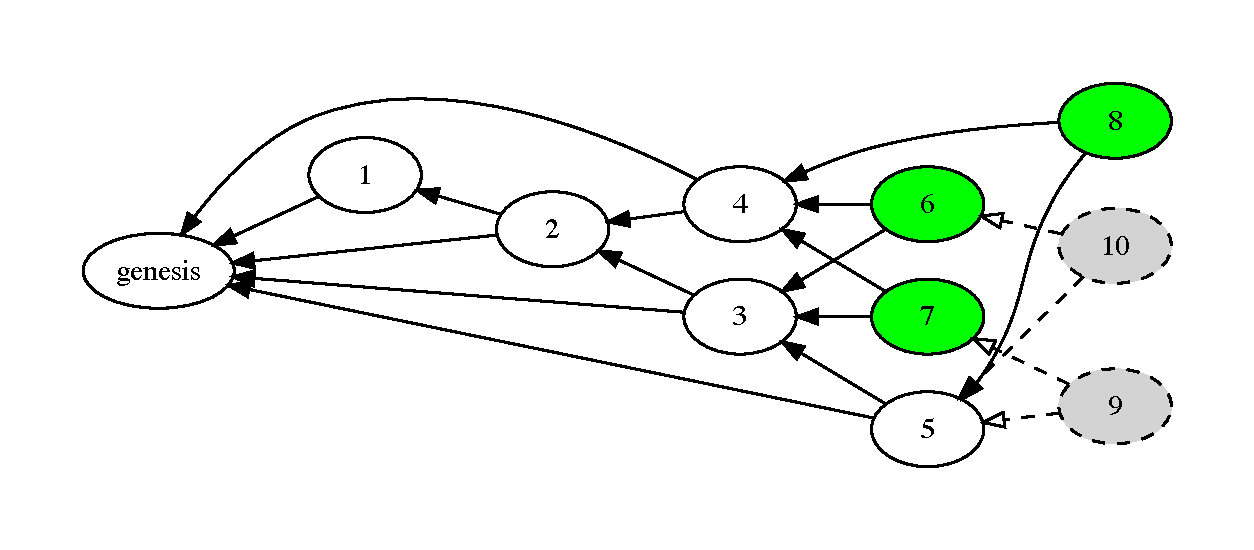
\includegraphics[width=\textwidth]{./images01/fig-tangle-example.pdf}
\caption{White nodes represent transactions that have been confirmed at least once. Green circles represent unconfirmed transactions (tips). Gray and dashed nodes are the transactions currently solving the proof-of-work in order to be propagated.\label{fig-tangle-example}}
\end{figure}

Transactions have an accumulated weight which may be interpreted as how hard it is to rollback a transaction. It is analogous to the number of confirmations of a block in Bitcoin. The higher the accumulated weight, the safer the transaction. Let $A$ be a transaction, its accumulated weight is the sum of all weights of the transactions which confirm $A$, including A itself, i.e., $w_A + \sum_{A \leadsto P} w_P$. For example, in Figure \ref{fig-tangle-example}, the accumulated weight of transaction 3 is the sum of the weights of the transactions 3, 5, 6, 7, and 8.

The score of a transaction is a measure of how much proof-of-work has been done before the transaction has been created. As the heighest score of the network increases over time, comparing a transaction's score with the highest score of the network indicates the ``age'' of the transaction. The score of a transaction A is the sum of all weights of the transactions which are being confirmed by A, including A itself, i.e., $w_A + \sum_{P \leadsto A} w_P$. For example, in Fig. \ref{fig-tangle-example}, the score of transaction 3 is the sum of the weights of the transactions 1, 2, and 3.

Another measure of the ``age'' of a transaction is its height. The height of a transaction A is the length of the longest path from transaction A to the genesis transaction. For example, in Fig. \ref{fig-tangle-example}, the height of transaction 5 is four ($5 \rightarrow 3 \rightarrow 2 \rightarrow 1 \rightarrow$ genesis). The lower the height, the older the transaction.

The depth of a transaction A is a measure of the youth of the transaction. It is the length of the longest path in the inverted graph from transaction A to any unconfirmed transaction (tip). For example, in Fig. \ref{fig-tangle-example}, the depth of transaction 2 is three ($2 \rightarrow 3 \rightarrow 5 \rightarrow 8$). It is the opposite of the height. The lower the depth, the younger the transaction. When a new transaction is confirming two transactions with high depth, it is referred to as lazy transaction.

The higher the volume of new transactions, the more unconfirmed transactions will appear. In Fig. \ref{fig-tangle-swarm}, the reader can notice that the number of new transactions was increased for a while, and then decreased back to the original value. The Iota has behaved well when exposed to a high load scenario, since it reduced the number of tips to only three after the high demand has ceased. It is like a moving swarm which gets wider when the number of new transactions increases and gets thinner when the number of new transactions decreases.

\begin{figure}[ht]
\centering
\includegraphics[width=\textwidth]{./images01/fig-tangle-swarm.pdf}
\caption{Suddenly the number of transactions per second increases and the width of the swarm grows. After a while, the number of transactions per second decreases and the width of the swarm shrinks.\label{fig-tangle-swarm}}
\end{figure}

Conflicting transactions may happen when two or more transactions try to spend the same tokens --- or, in the Bitcoin's transaction format, try to spend the same output. In this case, the network must choose which of the transactions will be accepted and the other one will be invalidated, even when both have already been confirmed. In fact, when one transaction is invalidated, the whole sub-DAG which confirms it is also invalidated. In this case, it may happen to reverse some transactions.

Intuitively, when there is a conflict, the network should accept the transaction which has greater accumulated weight, invalidating the others (see Fig. \ref{fig-tangle-conflict}). But it may be not enough to prevent some attacks like the nuclear submarine attack.

\begin{figure}[ht]
\centering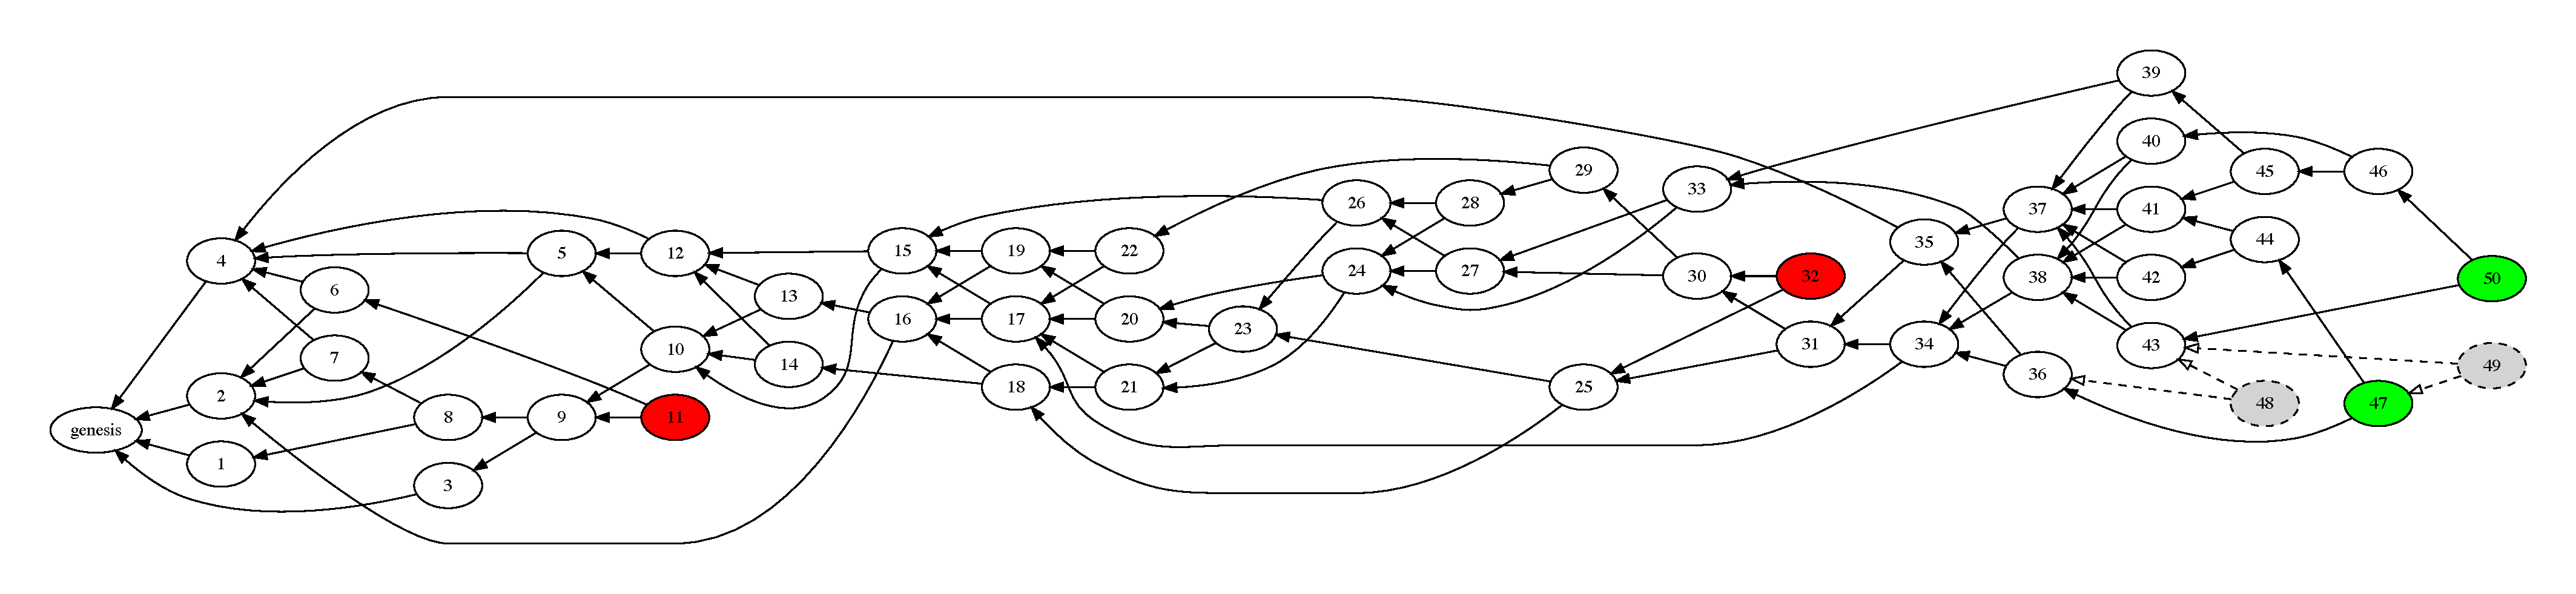
\includegraphics[width=\textwidth]{./images01/fig-tangle-conflict.pdf}
\caption{The red nodes are transactions which had some conflict with previous transaction and were invalidated by the network. Notice that none of them have been confirmed.\label{fig-tangle-conflict}}
\end{figure}

The nuclear submarine attack, also known as the parasite chain attack, is when the attacker generates a separate DAG (or a side DAG), with many transactions and a lot of proof-of-work. This side DAG is off the network, i.e., its transactions have not been propagated. Then, at a convenient moment, the attacker suddenly propagates these transactions. The whole network needs to decide how to handle these transactions.

If the transactions have no conflict with any transaction of the main DAG, i.e., there is no transaction spending the same tokens, then it is easy to handle the transactions. But, as it is an attack, there will be some conflicts, and it is not easy to choose which transaction should be invalidated. As the attacker has been generating a separate DAG, the conflicting transaction may have an accumulated weight similar or greater than the transaction which is already in the main DAG. Hence, using only the accumulated weight may not be enough to prevent this attack.

For example, the attackers generate (and do not propagate) a transaction that transfers all their funds to another address. Then, they start to generate many new transactions which confirm themselves and even confirm some of the transactions in the main DAG, but none of these transactions are also propagated to the network. Afterward, the attacker buys something in the real world, pays with cryptocurrency, and wait until the payment gets the accumulated weight demanded by the merchant. Finally, the attacker suddenly propagates all the transactions to the network in a small window of time. If the criteria is to validate the transaction with higher accumulated weight, the network will accept the attackers' original transaction instead of the one used to pay the merchant. Hence, the merchant transaction is invalidated, and the double spend attack has succeeded.

By default, Iota uses the Markov Chain Monte Carlo (MCMC) algorithm to select the two tips. For further information about attacks and strategies to prevent them, including the MCMC algorithm, see \cite{tangle2016}.

Next, I will do a mathematical analysis of Bitcoin in order to better understand its minings properties, how a fork would affect the network and its security against attackers. It is not necessary to do a mathematical analysis of Iota, because it has already been done in \citet{tangle2016}.


\chapter{Analysis of Bitcoin}
\label{ch:hathor-bitcoin-math}

The primary objective of this chapter is to increase our understanding of the Bitcoin through mathematical tools.

\section{Hash function}

Hash functions has been widely studied in computer science. In short, a hash function $h: \{0, 1\}^\infty \rightarrow \{0, 1\}^{n}$ has the following properties:

\begin{enumerate}
	\item $x = y \Rightarrow h(x) = h(y)$
	\item $h(x) \sim \mathcal{U}(0, 2^{n}-1)$, where $\mathcal{U}$ is the uniform distribution, i.e., $\forall a \in [0, 2^{n}-1], \mathbf{P}(h(x)=a) = \frac{1}{2^{n}}$
\end{enumerate}

In other words, when two inputs are the same, they have the same output. But, when the inputs are different, their outputs are uniformly distributed. Clearly, the hash functions are surjective but not injective. They are not injective because the image of $h$ has only $2^n$ elements and the domain has infinite elements. When $x \ne y$ and $h(x) = h(y)$, we say that $x$ and $y$ are a collision. A hash function is considered to be safe when it is unknown how to quickly find a collision of a given hash, i.e., one has to check all possible values until the correct one is found (known as the brute-force attack).

Bitcoin uses two hash functions: HASH-160 and HASH-256. The first has $n=160$ and consists of the composition of \textit{SHA-256} and \textit{RIPEMD-160}. The latter has $n=256$ and applies \textit{SHA-256} twice. The first is used in transactions' scripts and the latter in the mining algorithm. For both hash functions, it is infeasible to run a brute-force attack because it would demand, on average, either $2^{160}$ or $2^{256}$ trials, and those would take a tremendous amount of time even for the fastest known processors.

For further information about hash functions, see \citet{gilbert2003security, dobbertin1996ripemd}.


\section{Mining one block}

Let $\mathbb{B}$ be the set of Bitcoin blocks and $h: \mathbb{B} \rightarrow \{0, 1\}^{256}$ be the Bitcoin \textit{HASH-256} function. The mining process consists of finding $x \in \mathbb{B}$ such as $h(x) < A$, where $A$ is a given threshold. The smaller the $A$, the harder to find a new block. In fact, $\mathbf{P}(h(x) < A) = \frac{A}{2^{256}}$.

Hence, in order to find a new block, one must try different inputs ($x_1, x_2, \dots, x_k$) until they find a solution, i.e., all attempts will fail ($h(x_i) \geq A$ for $i < k$) but the last ($h(x_k) < A$). The probability of finding a solution exactly in the $k^{th}$ attempt follows a geometric distribution. Let $X$ be the number of attempts until a success, then $\mathbf{P}(X = k) = (1-p)^{k-1} p$, where $p = \frac{A}{2^{256}}$. Also, we have $\mathbf{P}(X \leq k) = 1 - (1-p)^k$. The average number of attempts is $\mathbf{E}(X) = 1/p$ and the variance is $\mathbf{V}(X) = \frac{1-p}{p^2}$.

In the Bitcoin's protocol, the given number $A$ is adjusted so that the network would find a new a block every 10 minutes, on average. Suppose that the Bitcoin's network is able to calculate $H$ hashes per second --- $H$ is the total hash rate of the network. The time required to find a solution would be $T=X/H$, and $\mathbf{E}(T) = \mathbf{E}(X)/H$ would be the average number of seconds to find a new block. So, the rule of finding a new block every 10 minutes ($\eta = 600$ seconds) --- on average --- leads to the following equation: $\mathbf{E}(T) = \eta = 600$. So, $\mathbf{E}(T) = \mathbf{E}(X)/H = \frac{1}{pH} = \eta = 600 \Rightarrow p = \frac{1}{\eta H}$. Finally, $\mathbf{E}(X) = \eta H$, $\mathbf{E}(T) = \eta$, $\mathbf{V}(X) = (\eta H)^2 - \eta H$, and $\mathbf{V}(T) = \eta^2 - \eta/H$.

The cumulative distribution function (CDF) of $T$ is $\mathbf{P}(T \leq t) = \mathbf{P}(X/H \leq t) = \mathbf{P}(X \leq tH) = 1 - (1-p)^{tH} = 1 - \left( 1-\frac{1}{\eta H} \right)^{tH}$. But, as the Bitcoin's network hash rate is really large, we may approximate the CDF of $T$ by $\lim_{H \rightarrow \infty} \mathbf{P}(T \leq t) = 1 - e^{-\frac{t}{\eta}}$, which is equal to the CDF of the exponential distribution with parameter $\lambda = \frac{1}{\eta}$.

\begin{theorem}
	When $H \rightarrow +\infty$, the time between blocks follows an exponential distribution with parameter $\lambda = \frac{1}{\eta}$, i.e., $\lim_{H \rightarrow +\infty} \mathbf{P}(T \leq t) = 1 - e^{-\frac{t}{\eta}}$.
\end{theorem}
\begin{proof}
\begin{align*}
	\mathbf{P}(T \leq t) &= 1 - (1-p)^{tH} \\
		     &= 1 - \left( 1 - \frac{1}{\eta H} \right)^{tH} \\
	\text{Replacing $u = \eta H$,} \\
	\lim_{H \rightarrow +\infty} \mathbf{P}(T \leq t) &= \lim_{u \rightarrow +\infty} 1 - \left( 1 - \frac{1}{u} \right)^{\frac{tu}{\eta}} \\
				&= \lim_{u \rightarrow +\infty} 1 - \left[ \left( 1 - \frac{1}{u} \right)^{u} \right]^{\frac{t}{\eta}} \\
				&= 1 - \left( 1/e \right)^{\frac{t}{\eta}} \\
				&= 1 - e^{-\frac{t}{\eta}}
\end{align*}
\end{proof}

Now, we would like to understand from which value of $H$ it is reasonable to assume that $T$ follows an exponential distribution.

\begin{theorem}
	$x > M \Rightarrow |(1+1/x)^x - e| < e/M$.
\end{theorem}
\begin{proof}
	Let's use the classical inequality $\frac{x}{1+x} < \log(1+x) < x$ for $x > -1$. So, $\frac{1/x}{1+1/x} < \log(1+x) < 1/x$. Simplifying, $\frac{1/x}{1+1/x} = 1/(1+x)$.  Thus, $1/(1+x) < \log(1+1/x) < 1/x \Rightarrow x/(1+x) < x \log(1 + 1/x) < 1$.

	As $\log(1 + \frac{1}{M}) > 0$ and $1 < 1 + \log(1 + \frac{1}{M})$.

	$x > M \Rightarrow 1/x < 1/M \Rightarrow 1+1/x < 1+1/M \Rightarrow 1/(1+1/x) > 1/(1+1/M) \Rightarrow x/(1+x) > M/(1+M)$.

	Again, $\log(1+x) < x \Rightarrow \log(1-1/M) < -1/M \Rightarrow 1 + \log(1-1/M) < (M-1)/M < M/(1+M)$, since $(x-1)/x < x/(x+1)$.

	Hence, $1 + \log(1-1/M) < M/(1+M) < x/(1+x) < x\log(1+1/x)$, and $x\log(1+1/x) < 1 < 1 + \log(1 + \frac{1}{M})$.

	Finally,

	\begin{align*}
		1 + \log(1-1/M) &< x\log(1+1/x) < 1 + \log(1 + \frac{1}{M}) \\
		e^{1 + \log(1-1/M)} &< e^{x\log(1+1/x)} < e^{1 + \log(1 + \frac{1}{M})} \\
		e \cdot e^{\log(1-1/M)} &< e^{\log((1+1/x)^x)} < e \cdot e^{\log(1 + \frac{1}{M})} \\
		e(1-1/M) &< (1+1/x)^x < e(1 + \frac{1}{M}) \\
		e-e/M &< (1+1/x)^x < e + e/M \\
		-e/M &< (1+1/x)^x - e < e/M \\
	\end{align*}
	Therefore, $\left| \left( 1+1/x \right)^x - e \right| < e/M$.
\end{proof}

We may consider $H$ big enough to say that $T$ follows an exponential distribution when $e/H < \epsilon$, where $\epsilon$ is the maximum approximation error. When $\epsilon = 10^{-6} \Rightarrow H > e \cdot 10^6$. So, when $H > 2.6 \text{Mh/s}$, our approximation is good enough.

The symmetrical confidence interval with level $\alpha$ would be $[t_0, t_1]$, where $\mathbf{P}(t_0 < T < t_1) = 1-\alpha$, $\mathbf{P}(T<t_0) = \alpha/2$, and $\mathbf{P}(T>t_1) = \alpha/2$. These conditions give the following equations: $1 - e^{-t_0/\eta} = \alpha/2$, and $e^{-t_1/\eta} = \alpha/2$. Solving these equations, we have $t_0 = -\eta \ln{(1 - \alpha/2)}$, and $t_1 = -\eta \ln{(\alpha/2)}$.

For instance, if $\alpha = 10\%$, then $t_0 = 30.77$ and $t_1 = 1797.44$ (or $[0.51, 30.76]$ in minutes). Thus, 90\% of the time the intervals between blocks are between 30 seconds and 30 minutes, with average of 10 minutes.

The fact that the time between blocks follows an exponential distribution with $\lambda = 1/\eta = pH$ may be used to estimate the total network's hash rate (or a miner's hash rate). For further information, see \cite{ozisikestimation}.


\section{Mining several blocks}

Let $T_1, T_2, T_3, \dots, T_n$ be the time to find the first block ($T_1$), then the time to find the second block ($T_2$), and so on. Let's analyze the distribution of $Y_n = \sum_{i=1}^{n} T_i$ which is the total time to find the next $n$ blocks. As $Y_n$ is the sum of random variables which follow an exponential distribution with same $\lambda = \frac{1}{\eta}$, then $Y_n \sim \text{Erlang}(n, \frac{1}{\eta})$. Thus, the CDF of $Y$ would be $\mathbf{P}(Y_n < t) = 1 - \sum_{k=0}^{n-1} \frac{1}{k!} e^{-\lambda t} (\lambda t)^k$.

Many exchanges require at least six confirmations in order to accept a deposit in Bitcoin. So, for $n=6$, $\mathbf{P}(Y_6 < 1 \text{ hour}) = \mathbf{P}(Y_6 < 3600) = 0.5543$, i.e., only 55\% of the deposits will be accepted in one hour. The symmetrical confidence interval with $\alpha=10\%$ is $[27, 105]$ in minutes. Thus, 90\% of the times, it will take between 27 minutes and 1 hour and 45 minutes to have your deposit accepted --- assuming that your transaction will be confirmed in the very next block. The pdf of $Y_6$ is shown in Figure \ref{fig-bitcoin-time-6-blocks}, in which the 10\% symmetrical confidence interval is shown in the white area. The average total time of six confirmations is $\mathbf{E}(Y_6) = 6 \cdot 600 = 3600 = 60 \text{ minutes}$.

\begin{figure}[ht]
\centering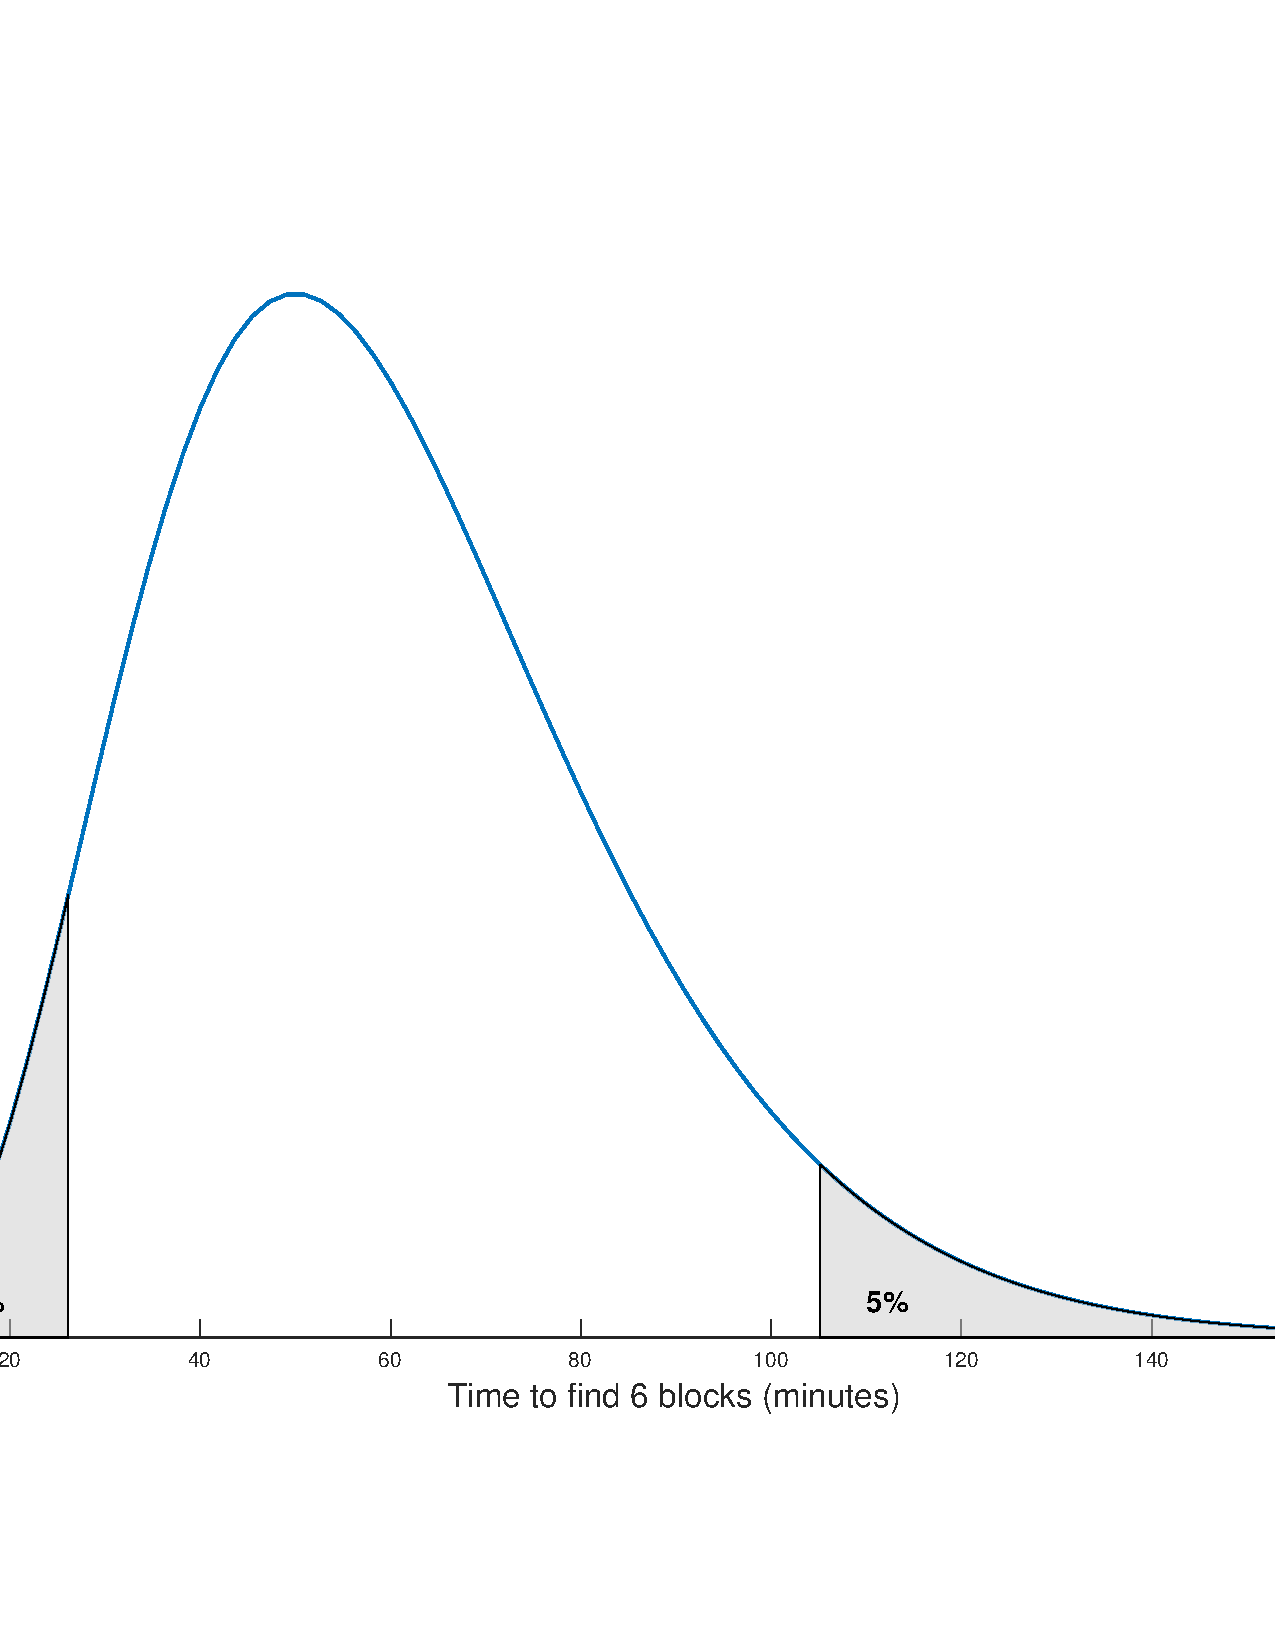
\includegraphics[width=\textwidth]{./images01/time-6-blocks.pdf}
\caption{Probability density function of $Y_6$, i.e., probability of finding 6 blocks after time $t$. The shaded areas shows the lower 5\% and upper 5\% of the pdf.\label{fig-bitcoin-time-6-blocks}}
\end{figure}

\section{Mining for a miner}

Let's analyze the probability of finding a new block for a miner who has $\alpha$ percent of the network's total hash rate. Let $T_\alpha = \frac{X}{\alpha H}$ be the time required for the miner to find a new block. As $T_\alpha = \left( \frac{1}{\alpha} \right) T$, when $H \rightarrow +\infty$, $T_\alpha$ also follows an exponential with parameter $\lambda_\alpha = \frac{\alpha}{\eta}$. Hence, we confirm the intuition that the miner with $\alpha$ percent of the network's total hash power will find $\alpha$ percent of the blocks.

\begin{theorem}
	When the miner with $\alpha$ percent of the network's total hash rate is part of the mining network, $\mathbf{P}(\text{next block is from $T_\alpha$}) = \alpha.$
\end{theorem}
\begin{proof}
\begin{align*}
	\mathbf{P}(\text{next block is from $T_\alpha$}) &= P \left( T_\alpha = \min\{T_\alpha, T_{1-\alpha}\} \right) \\
		&= \frac{\lambda_\alpha}{\lambda_\alpha + \lambda_{1-\alpha}} \\
		&= \frac{\alpha/\eta}{\alpha/\eta + (1-\alpha)/\eta} \\
		&= \frac{\alpha}{\alpha + 1 - \alpha} \\
		&= \alpha.
\end{align*}
\end{proof}

\begin{theorem}
	When one miner with $\alpha$ percent of the network's total hash rate multiplies their hash rate by $m$, the probability of this miner find the next block is multiplied by $\frac{m}{m \alpha + 1 - \alpha}$.
	\label{thm-miner-multiply}
\end{theorem}
\begin{proof}
	When miners increase their hash rate, they also increase the network's total hash rate. Let $H$ be the network's hash rate before the increase. Thus, the network's total hash rate after the increase is $H + (m-1) \alpha H = (1 - \alpha + m \alpha) H$. So,
\begin{align*}
	\mathbf{P}(\text{next block is from $T_{m \alpha}$}) &= P \left( T_{m \alpha} = \min\{T_{m \alpha}, T_{1-\alpha}\} \right) \\
		&= \frac{\lambda_{m \alpha}}{\lambda_{m \alpha} + \lambda_{1-\alpha}} \\
		&= \frac{m \alpha/\eta}{m \alpha/\eta + (1-\alpha)/\eta} \\
		&= \frac{m \alpha}{m \alpha + 1-\alpha} \\
		&= \alpha \left( \frac{m}{m \alpha + 1 - \alpha} \right).
\end{align*}
\end{proof}

\begin{cor}
	If one miner has a really tiny percent of the network's total hash rate, then multiplying their hash rate by $m$ approximately multiplies their probability of finding the next block by $m$.
\end{cor}
\begin{proof}
	$$\lim_{\alpha \rightarrow 0} \mathbf{P}(\text{next block is from $T_{m \alpha}$}) = \lim_{\alpha \rightarrow 0} \frac{m}{m \alpha + 1 - \alpha} = m.$$
\end{proof}

That way, it is not exactly correct to say that when one doubles their hash rate, their probability will double as well. It is only true for small miners.


\section{Orphan blocks}
% Probabilidade de orfão
An orphan block would be created if a new block is found during the propagation time of a new block. Let $\alpha$ be the percentage of the total hash rate of the node which is outdated, and $\Delta t$ the propagation time in seconds. Thus, $\mathbf{P}(\text{new orphan}) = \mathbf{P}(T < \Delta t) = 1 - e^{-\frac{\alpha \Delta t}{\eta}}$.

Bitcoin peer-to-peer network is a gossip network, where miners are semi-randomly connected to each other, and each miner sends all information it receives to all its peers. According to \citet{decker2013information}, the average time for a new block propagate over the network is 12.6 seconds, while the 95\% percentile is 40 seconds, which indicates a long-tail distribution. \citet{bitcoinstats} has measured the propagation time between 2013 and 2017. During 2017, the worst daily 90\% percentile was 21 seconds. Notice that both results may not be contradictory because Bitcoin network is continuously evolving.

For instance, if a node has 10\% of the total hash rate and it takes 30 seconds to receive the update, then $\mathbf{P}(\text{new orphan}) = 1 - e^{-\frac{0.1 \cdot 30}{600}} = 0.004987$, which is almost 0.5\%. I would say that a node with 10\% of the total hash rate would be well connected and it would take less time to receive the update, so, the probability would be even smaller than 0.5\%.

Another important factor is that, as Bitcoin is open-source, miners are free to change the gossip algorithm, which leads to the network incentives. See \citet{babaioff2012bitcoin} for an analysis of the incentives to miners forward new blocks and transactions in the network.

For further information about gossip algorithms, see \citet{shah2009gossip}.


\section{Analysis of network's hash rate change}
% Análise: Mudança no network's hash rate antes de atualizar o $A$.

The difficulty, given by the number $A$, is adjusted every 2016 blocks. As, $\mathbf{P}(13 \text{ days} < Y_{2016} < 15 \text{ days}) = \mathbf{P}(13 \cdot 24 \cdot 3600 < Y_{2016} < 14 \cdot 24 \cdot 3600) = 0.9986$, it is expected that the total time to find 2016 blocks will be between 13 and 15 days, assuming that the network's hash rate remains constant. If it takes less than the expected time, it means that the network's total hash rate has increased. While if it takes more than the expected time, it means that the network's total hash rate has decreased. So, let's analyze what happens when the network's hash rate changes significantly.

%Let's assume that the network's total hash rate will change only once, from $H$ to $\alpha H$ --- so, if $\alpha = 1$, there would be no change, if $\alpha > 1$, there would be an increase, and if $\alpha < 1$, there would be a decrease. As the time required to find a new block would be $T_\alpha = \frac{X}{\alpha H}$, we got the same random variable as we have gotten when analyzing a miner with $\alpha$ percent of the network's total hash rate. But, the analysis will be different because here $\alpha$ may be greater than one.

Let $H \cdot u(t)$ be the network's total hash rate over time. So, the number of hashes calculated in $t$ seconds is $H \int_0^t u(t) dt$. Hence, $\mathbf{P}(T \leq t) = \mathbf{P}(X \leq H \int_0^t u(t)dt)$. When $H \rightarrow +\infty$, $\mathbf{P}(T \leq t) = 1 - e^{-\frac{1}{\eta} \int_0^t u(t) dt}$, and the pdf of $T$ is $\frac{u(t)}{\eta} \cdot e^{-\frac{1}{\eta} \int_0^t u(t)dt}$.

Let's say that the network's total hash rate has suddenly multiplied by $\alpha$. So, $u(t) = \alpha$, $\int_0^t u(t) dt = \alpha t$, and $T$ also follows an exponential distribution, but with $\lambda = \frac{\alpha}{\eta}$. Thus, $Y_n^\alpha = \sum_{i=1}^{n} T_i^\alpha \sim \text{Erlang}(n, \frac{\alpha}{\eta})$. Thus, $\mathbf{E}[Y_{n}^\alpha] = \frac{\mathbf{E}[Y_{n}]}{\alpha}$, i.e., the average total time required to find $n$ blocks will be divided by $\alpha$, while $\mathbf{V}[Y_{n}^\alpha] = \frac{\mathbf{V}[Y_n]}{\alpha^2}$ and the variance will be divided by $\alpha^2$. Hence, on one hand, when the network's hash rate increases ($\alpha > 1$), the 2016 blocks will be found earlier. On the other hand, when the network's hash rate decreases ($\alpha < 1$), the 2016 blocks will be found later.

For example, if the network's total hash rate suddenly doubles ($\alpha = 2$), then $\mathbf{P}(6.5 \text{ days} < Y_{2016} < 7.5 \text{ days}) = 0.9986$, and the time required to find 2016 blocks halved. On the other side, if the network's total hash rate suddenly halves ($\alpha = 0.5$), then $\mathbf{P}(27 \text{ days} < Y_{2016} < 29 \text{ days}) = 0.9469$, and the time required to find 2016 blocks doubled. It is an important conclusion, since it shows that even if half of the network stops mining, it will only double the time to the next difficulty adjustment, i.e., the time between blocks will be 20 minutes for, at most, the next 29 days, at which point the adjustment will occur and everything will be back to the normal 10 minutes between blocks.

% TODO Step-wise analysis

\subsection{Hash rate smoothly changing}

Let $u(t) = \frac{1+abx}{1+bx}$. It is an useful function because $u(0) = 1$ and $\lim_{t \rightarrow \infty} u(t) = a$. The bigger the $b$, the faster $u(t) \rightarrow a$. For example, if $a=2$, it means $H$ would be smoothly doubling. If $a=0.5$, it means $H$ would be smoothly halving.

It is easy to integrate $u(t)$ because $\frac{1+abx}{1+bx} = \frac{1-a}{1+bx} + a \Rightarrow \int_0^t u(x) dx = at + \frac{1-a}{b} \log(1+bt)$. So,
$$F_T(t) = 1 - (1+bt)^{\frac{\lambda(a-1)}{b}} e^{-\lambda at}.$$
$$f_T(t) = \lambda \left( \frac{1+abt}{1+bt} \right) (1+bt)^{\frac{\lambda(a-1)}{b}} e^{-\lambda at}.$$

Assuming that $n = \frac{\lambda(a-1)}{b}$ is integer, we have:
$$F_T(t) = 1 - (1+bt)^n e^{-\lambda at}$$

Thus,
\begin{align*}
\mathcal{L}\{F_T(t)\} &= \mathcal{L}\{1 - (1+bt)^n e^{-\lambda at}\} \\
	&= \mathcal{L}\{1\} - \mathcal{L}\{(1+bt)^n e^{-\lambda at}\} \tag{$\mathcal{L}$ is a linear operator} \\
	&= \frac{1}{s} - \mathcal{L}\{(1+bt)^n e^{-\lambda at}\} \\
	&= \frac{1}{s} - \sum_{k=0}^n \binom{n}{k} b^k \mathcal{L}\{t^k e^{-\lambda at}\} \\
	&= \frac{1}{s} - \sum_{k=0}^n \binom{n}{k} b^k \frac{k!}{(s+\lambda a)^{k+1}}
\end{align*}

Hence, as $\mathcal{L}\{f_T(t)\} = s \mathcal{L}\{F_T(t)\}$,

$$\mathcal{L}\{f_T(t)\} = 1 - \sum_{k=0}^n \binom{n}{k} \frac{s b^k k!}{(s+\lambda a)^{k+1}}$$

Then,

\begin{align*}
\frac{d}{ds} \mathcal{L}\{f_T(t)\}
	&= - \sum_{k=0}^n \binom{n}{k} b^k k! \frac{d}{ds} \frac{s}{(s+\lambda a)^{k+1}} \\
	&= - \sum_{k=0}^n \binom{n}{k} b^k k! \left[ \frac{1}{(s+a\lambda)^{k+1}} - \frac{s(k+1)}{(s+a \lambda)^{k+1}} \right] \\
\frac{d}{ds} \mathcal{L}\{f_T(t)\}|_{s=0}
	&= - \sum_{k=0}^n \binom{n}{k} b^k k! \frac{1}{(\lambda a)^{k+1}} \\
	&= - \frac{1}{a\lambda} \sum_{k=0}^n \binom{n}{k} k! \left( \frac{b}{\lambda a} \right)^k \\
	&= - \frac{1}{a\lambda} \sum_{k=0}^n \frac{n!}{(n-k)!} \left( \frac{b}{\lambda a} \right)^k \\
	&= - \frac{1}{a\lambda} \left[ n! \sum_{k=0}^n \frac{1}{(n-k)!} \left( \frac{b}{\lambda a} \right)^k \right] \\
	&= - \frac{1}{a\lambda} \left[ n! \sum_{k=0}^n \frac{1}{k!} \left( \frac{b}{\lambda a} \right)^{n-k} \right] \tag{$k \rightarrow n-k$} \\
	&= - \frac{1}{a\lambda} \left[ n! \left(\frac{b}{\lambda a}\right)^n \sum_{k=0}^n \frac{1}{k!} \left( \frac{b}{\lambda a} \right)^{-k} \right] \\
	&= - \frac{1}{a\lambda} \left[ n! \left(\frac{b}{\lambda a}\right)^n \sum_{k=0}^n \frac{1}{k!} \left( \frac{\lambda a}{b} \right)^{k} \right]
\end{align*}

Finally, as $\mathbf{E}[T] = -\mathcal{L}\{f_T(t)\}|_{s=0}$,
$$\mathbf{E}[T] = \frac{1}{\lambda a} \left[ n! \left(\frac{b}{\lambda a}\right)^n \sum_{k=0}^n \frac{1}{k!} \left( \frac{\lambda a}{b} \right)^{k} \right] \text{, where $n = \frac{\lambda(a-1)}{b}$}$$

Let's check this equation for already known scenarios. When $a=1$, then $n=0$ and $\mathbf{E}[T] = 1/\lambda$. When $b \rightarrow +\infty$, it reduces to the case in which the hash rate is multiplied by $a$, which we have already studied. In fact, $n \rightarrow 0$, $u(t) \rightarrow a$, and $\mathbf{E}[T] = \frac{1}{\lambda a}$.

\begin{theorem}
	$$a > 1 \text{ and } x > M \Rightarrow \left| \frac{1+abx}{1+bx} - a \right| < \frac{a-1}{1+bM}$$
\end{theorem}
\begin{proof}
$x > M \Rightarrow \frac{1}{1+bx} < \frac{1}{1+bM}$. As $1-a<0$, $\frac{1-a}{1+bx} > \frac{1-a}{1+bM}$. Thus, $\frac{1-a}{1+bM} < \frac{1-a}{1+bx} + a - a = \frac{1+abx}{1+bx} - a < 0 < \frac{a-1}{1+bM}$. Hence, $-\frac{a-1}{1+bM} < \frac{1+abx}{1+bx} - a < \frac{a-1}{1+bM}$.
\end{proof}

For instance, if we would like to know the impact of smoothly double the hash rate in the next week, then the parameters would be $\lambda = 1/600$, $a=2$, $M=1\text{ week}=3600\cdot24\cdot7 = 604,800$, $b$ can be calculated using $\epsilon = \frac{a-1}{1+bM} < 0.01 \Leftarrow b > 0.000163690 \Leftarrow n < 10.1818$. So, for $n=10$, then $b=0.000166666$ and $\epsilon = 0.009823 < 0.01$, as expected. Finally, $\mathbf{E}[T] = 557.65$. In other words, during the next week, the average time between blocks will be 9 minutes and 17 seconds, instead of the normal 10 minutes. If the hash rate had suddenly doubled, the average time between blocks would be 5 minutes.

%$$\mathbf{E}[T] = -\mathcal{L}\{f_T(t)\}|_{s=0} = \frac{b^n n! 600^{n+1}}{a^{n+1}} e^{\frac{a}{600b}} \text{, where $n = \frac{a-1}{600b}$}$$


%$a > 1, x > M \Rightarrow 1 + bx > 1 + bM \Rightarrow \frac{1}{1+bx} < \frac{1}{1+bM} \Rightarrow \frac{1-a}{1+bx} + a > \frac{1-a}{1+bM} + a \Rightarrow \frac{1+abx}{1+bx} - a > \frac{1-a}{1+bM}$.


\subsection{Piecewise linear model of hash rate change}

Let's analyze what would happen if the network's hash rate is growing linearly with angular coefficient $a^2$, i.e., $u(a, b, t) = a^2t + b$. Thus, $\mathbf{P}(T \leq t) = 1 - e^{-\frac{bt + a^2t^2/2}{\eta}}$.

It is well known that $\mathbf{E}(T) = \int_{0}^{\infty} 1 - \mathbf{P}(T \leq t) dt$. Thus, replacing $y = \frac{a^2 t + b}{a \sqrt{2 \eta}}$, and using the fact that $\int_0^\infty e^{-x^2} dx = \frac{\sqrt{\pi}}{2} \erf(x)$, we have:

\begin{align}
\mathbf{E}(T)|_{t_1}^{t_2} &= \int_{t_1}^{t_2} \exp \left( - \frac{bt + a^2 t^2/2}{\eta} \right) dt \nonumber \\
	&= \frac{\sqrt{2 \eta}}{a} \exp \left( \frac{b^2}{2a^2 \eta} \right) \int_{y_1}^{y_2}  \exp(-y^2) dy \nonumber \\
	&= \frac{\sqrt{2 \eta}}{a} \exp \left( \frac{b^2}{2a^2 \eta} \right) \frac{\sqrt{\pi}}{2} [\erf(y_1) - \erf(y_2)] \nonumber \\
	&= \frac{\sqrt{2 \pi \eta}}{2a} \exp \left( \frac{b^2}{2a^2 \eta} \right) \left[\erf(y_2) - \erf(y_1) \right]
\end{align}

Where $y_1 = \frac{a^2 t_1 + b}{a \sqrt{2 \eta}}$ and $y_2 = \frac{a^2 t_2 + b}{a \sqrt{2 \eta}}$.

Thus, $\mathbf{E}(T) = \mathbf{E}(T)|_0^\infty$. When $t_1 = 0 \Rightarrow y_1 = \frac{b^2}{2 \sqrt{2 \eta}}$ and $t_2 \rightarrow \infty \Rightarrow y_2 \rightarrow \infty \Rightarrow \erf(y_2) = 1$, then:

$$
\mathbf{E}(T) = \frac{\sqrt{2 \pi \eta}}{2a} \exp \left( \frac{b^2}{2a^2 \eta} \right) \left[1 - \erf\left(\frac{1}{a \sqrt{2 \eta}}\right)\right]
$$

The function $\mathbf{E}(T)|_{t_1}^{t_2}$ may be used to a piecewise linear analysis of any hash rate change. Let's analyze the hash doubling in one week. Then, $u(1 \text{week}) = u(604800) = 2$, thus $a^2 = \frac{1}{604800} \Rightarrow a = \frac{1}{120 \sqrt{42}}$. Let's sample the interval $[0, 1 \text{week}]$ every hour, i.e., ($t_0$, $t_1$, $t_2$, \dots, $t_168$), where $t_i = i \cdot 1 \text{hour} = i \cdot 3600$.

For each point $t_i$, let $g_i(t) = [H(t-t_i) - H(t-604800)] u(t) + 2 H(t-604800)$, then $\mathbf{E}(T) = \mathbf{E}(T)|_{t_i}^{t_{i+1}} + 1 - e^{\frac{t}{\eta}}$. The result is presented in Figure .

%In order to obtain $\mathbf{E}(T)$, we will use the formula $\frac{d}{ds}T^*(s)|_{s=0} = -\mathbf{E}(T)$, where $T^*$ is the Laplace transform of the pdf of T.
%
%Let $f_T(x)$ be the pdf of T and $F_T(x)$ be the cdf of T, i.e., $F_T(x) = \int_0^x f_T(t) dt$. Thus, $\mathcal{L}\{F_T(x)\} = \frac{T^*(s)}{s}$.
%
%\begin{align*}
%	\mathcal{L}\{F_T(x)\} &= \int_0^\infty e^{-sx} F_T(x) dx \\
%		&= \int_0^\infty e^{-sx} \left( 1 - e^{-\frac{x + a^2x^2/2}{\tau}} \right) dx \\
%		&= \int_0^\infty e^{-sx} dx - \int_0^\infty e^{-sx} e^{-\frac{x + a^2x^2/2}{\tau}} dx \\
%		&= \frac{1}{s} - \int_0^\infty e^{-sx -\frac{x + a^2x^2/2}{\tau}} dx \\
%\end{align*}
%
%Let $b=\frac{a}{\sqrt(2 \tau)}$ and $c = \frac{\sqrt(2 \tau)}{2a} \left( s + \frac{1}{\tau} \right)$, then $sx + \frac{x+a^2x^2/2}{\tau} = (bx + c)^2 - c^2$.
%Let $y = bx+c \Rightarrow dy = bdx$.
%
%\begin{align*}
%	\int_0^\infty e^{-sx -\frac{x + a^2x^2/2}{\tau}} dx &= \int_0^\infty e^{-(bx+c)^2 + c^2} dx \\
%		&= \int_c^\infty e^{-y^2 + c^2} \frac{dy}{b} \\
%		&= \frac{e^{c^2}}{b} \int_c^\infty e^{-y^2} dy \\
%		&= \frac{\sqrt{\pi}e^{c^2}}{2b} \erfc(c)
%\end{align*}
%
%$$ \mathcal{L}\{F_T(x)\} = \frac{1}{s} - \frac{\sqrt{\pi}e^{c^2}}{2b} \erfc(c) $$
%
%Hence,
%$$ T^*(s) = s \mathcal{L}\{F_T(x)\} = 1 - \frac{s\sqrt{\pi}e^{c^2}}{2b} \erfc(c) $$
%
%As $\frac{d}{ds}c = \frac{\sqrt{2 \tau}}{2a}$,
%
%\begin{align*}
%\frac{d}{ds} T^*(s) &= - \frac{\sqrt{\pi}e^{c^2}}{2b} \erfc(c) - \frac{\sqrt{2 \tau \pi} sc e^{c^2}}{2ab} \erfc(c) + \frac{\sqrt{2 \tau \pi}s}{4ab} \\
%\frac{d}{ds} T^*(s)|_{s=0} &= - \frac{\sqrt{2 \tau \pi}}{2a} e^{\frac{1}{2 \tau a^2}} \erfc\left(\frac{1}{a \sqrt{2 \tau}}\right) \\
%\mathbf{E}[T] &= \frac{\sqrt{2 \tau \pi}}{2a} e^{\frac{1}{2 \tau a^2}} \erfc\left(\frac{1}{a \sqrt{2 \tau}}\right) \\
%\end{align*}
%
%$\mathbf{E}[T]$ is ploted for $a \in (0, 0.1]$ at Figure \ref{fig-bitcoin-H-increase}. The plot interval is really small because $a=1$ would imply doubling the hash rate after 1 second.
%
%\textcolor{red}{I do not know how to interpret this.}

\begin{figure}[ht]
\centering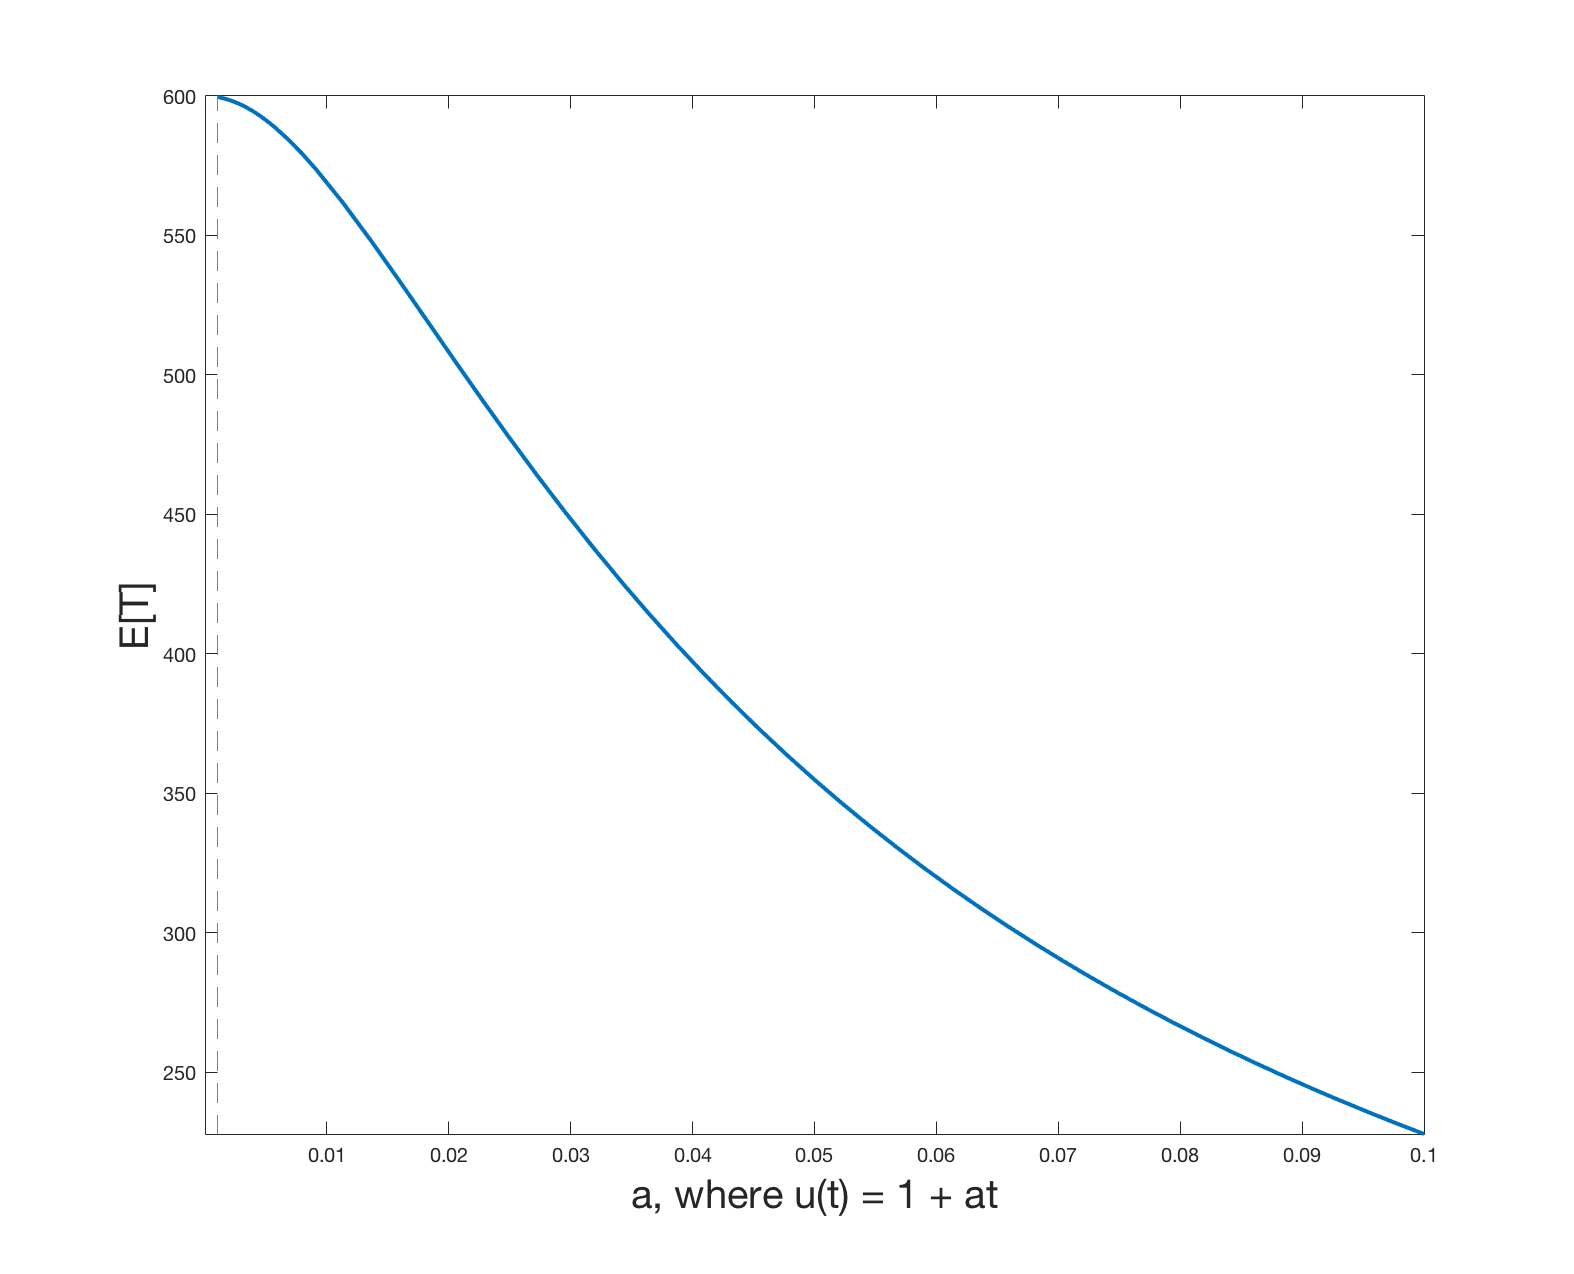
\includegraphics[width=\textwidth]{./images01/bitcoin-H-increasing.png}
\caption{$\mathbf{E}[T]$ when H increases linearly with $u(t) = 1 + at$.\label{fig-bitcoin-H-increase}}
\end{figure}


\section{Attack in the Bitcoin network}
% Ataque submarino
% Probabilidade de "correr por fora"

\citet{karame2012two}

There are many possible ways to attack the Bitcoin (REF). In this section, we are interested in a particular attack: the double spending attack.

In the double spending attack, the attacker's send some funds to the victim, let's say a merchant. They wait for $k$ confirmations of the transaction, and the victim delivers the good or the service to the attacker. Then, the attacker mine enough blocks with a conflicting transaction, double spending the funds which was sent to the victim. If the attacker is successful, the original transaction will be \textit{erased} and the victim will be left with no funds at all. In order to be successful, the attacker must propagate more blocks than the network in the same period, propagating a chain longer than the main chain. Hence, we would like to understand what the odds are that the attacker will be successful. This attack was originally discussed by \citet{nakamoto2008bitcoin}.

In order to maximize their odds, the attacker must start to mine the new blocks as soon as they send the funds to the victim. In this moment, it starts to mine in the head of the blockchain, just like the rest of the network. So, in the beginning, the attacker and the network are in exactly the same point.

Let $\beta H$ be the hash rate of the attackers, and $\gamma H$ be the network's hash rate without the attackers. Thus, when $H \rightarrow +\infty$, we already know that $T_{\text{attackers}}$ and $T_{\text{network}}$ follow exponential distributions with parameters $\lambda_{\text{attacker}} = \frac{\beta}{\eta}$ and $\lambda_{\text{network}} = \frac{\gamma}{\eta}$, respectively.

As \cite{nakamoto2008bitcoin} has done, we will also model the attack using the Gambler's Ruin. In this game, a gambler wins \$1 at each round, with probability $p$, and loses \$1, with probability $1-p$. The rounds are independent. The gambler starts with \$$k$ plays continuously until he either accumulates a target amount of \$$m$, or loses all his money. Let $\rho = \frac{1-p}{p}$, then the probability of losing his fortune is:

$$
\mathbf{P}(\text{losing his fortune}) =
\begin{cases}
	\frac{\rho^k - \rho^m}{1-\rho^m} \text{, if $\rho \ne 1$,} \\
	\frac{m-k}{m} \text{, if $\rho = 1$.}
\end{cases}
$$

When $m \rightarrow +\infty$,

$$
\mathbf{P}(\text{losing his fortune}) =
\begin{cases}
	\rho^k \text{, if $\rho < 1$,} \\
	1 \text{, if $\rho \geq 1$.}
\end{cases}
$$

% TODO Expected time to absorption.

The gambler winning \$1 is the same as the network finding a new block, the gambler losing \$1 is the same as the attacker finding a new block. The initial \$$k$ is the same as the number of blocks the attacker is behind the network. Thus, the gambler loses his fortune is the same as the attacker successfully finds $k$ or more blocks than the network, i.e., losing his fortune means that the attack was successful.

In our case, $p = \frac{\lambda_{\text{network}}}{\lambda_{\text{network}} + \lambda_{\text{attacker}}} = \frac{\gamma}{\beta + \gamma}$, thus $\rho = \frac{\beta}{\gamma}$. Hence, $\rho < 1 \Leftrightarrow \beta < \gamma$.

Suppose that the attacker is mining with the network. Suddently, he stops mining with the network and starts attacking, i.e., starts to mine in another chain. In this scenario, since the attacker's hash rate is not mining with the network anymore, $\gamma = 1 - \beta$. Thus, $\beta < \gamma \Rightarrow \beta < 0.5 \Leftrightarrow \rho < 1$. Here comes the conclusion that, if the attacker has 50\% or more of the network's hash rate, then his attack will be certainly successful. We got exactly the same equations and conclusions as \cite{nakamoto2008bitcoin}.

But this scenario seems not to be the optimal attack, because the attacker has waited $k$ confirmations before starting the attack. A better approach would be to start attacking just after propagating the transaction. In this case, our previous model is not good, because even if the attacker have found more blocks than the network, he cannot propagate those blocks before the network has found $k$ confirmations. So, we have to model the probabilities before the network has found the $k$ block. Then, if the attacker has more blocks than the network, he has successfully attacked. Otherwise, we return to the previous model, in which the attacker must still find more blocks.

\begin{theorem}
	Assuming that the attacker starts the attack just after publishing the transaction, the probability of the attacker has already found exactly $s$ blocks while it waits the network to find $k$ blocks is $\mathbf{P}(S = s) = \binom{k+s-1}{s} (1-p)^s p^k.$
\end{theorem}
\begin{proof}
The attacker must find exactly $s$ blocks while the network must find exactly $k$ blocks. It is as they would be walking the grid from the point $(0, 0)$ to $(s, k)$, where it is only allowed to go up or right, like in Figure \ref{figure:bitcoin-attack-paths}. When the attacker finds a block, it would be a movement to the right. When the network finds a block, it would be an upward movement. No matter the order which the blocks are found, all the paths occur with probability $(1-p)^s p^k$.

The walking ends when $(\cdot, k$) is reached, i.e., when the network finds $k$ blocks, regardless of how many blocks the attacker has found -- i.e., it is not allowed to walk above the line $(\cdot, k)$. Thus, the number of paths between $(0, 0)$ and $(s, k)$ moving only upward or to the right, without going into the line $(\cdot, k)$ is exactly the number of paths between $(0, 0)$ and $(s, k-1)$, which is equal to the number of permutations of the sequence $(u, u, \dots, u, r, r, \dots, r)$ in which there are $s$ movements to the right ($r$) and $k-1$ upward movements ($u$). This number of permutations is $\frac{(k-1+s)!}{s!(k-1)!} = \binom{(k-1)+(s)}{s}$ because there are $s$ repetitions of the element $r$ and $k-1$ repetitions of the element $u$.

Finally, the probability is $\binom{k+s-1}{s} (1-p)^{s} p^{k}$.

\begin{figure}[ht]
  \centering
  \begin{tikzpicture}
    \coordinate (Origin)   at (0,0);
    \coordinate (XAxisMin) at (-1,0);
    \coordinate (XAxisMax) at (5,0);
    \coordinate (YAxisMin) at (0,-1);
    \coordinate (YAxisMax) at (0,5);
    %\draw [thin, gray,-latex] (XAxisMin) -- (XAxisMax);% Draw x axis
    %\draw [thin, gray,-latex] (YAxisMin) -- (YAxisMax);% Draw y axis

    \clip (-0.5,-0.5) rectangle (10.5cm,7cm); % Clips the picture...
    %\pgftransformcm{1}{0}{0}{1}{\pgfpoint{0cm}{0cm}}
          % This is actually the transformation matrix entries that
          % gives the slanted unit vectors. You might check it on
           % MATLAB etc. . I got it by guessing.
    \draw[style=help lines,dashed] (0,0) grid[step=1cm] (14,6);
          % Draws a grid in the new coordinates.
          %\filldraw[fill=gray, fill opacity=0.3, draw=black] (0,0) rectangle (2,2);
              % Puts the shaded rectangle
    \foreach \x in {0,1,...,10}{% Two indices running over each
      \foreach \y in {0,1,...,6}{% node on the grid we have drawn
        \node[draw,circle,inner sep=1pt,fill] at (\x,\y) {};
            % Places a dot at those points
      }
    }

    \draw [ultra thick,-latex,red] (0,0) -- (0,1) node [midway, left] {};
    \draw [ultra thick,-latex,red] (0,1) -- (0,2) node [midway, left] {};
    \draw [ultra thick,-latex,red] (0,2) -- (1,2) node [midway, above] {};
    \draw [ultra thick,-latex,red] (1,2) -- (1,3) node [midway, right] {};
    \draw [ultra thick,-latex,red] (1,3) -- (2,3) node [midway, right] {};
    \draw [ultra thick,-latex,red] (2,3) -- (2,4) node [midway, right] {};
    \draw [ultra thick,-latex,red] (2,4) -- (2,5) node [midway, right] {};
    \draw [ultra thick,-latex,red] (2,5) -- (3,5) node [midway, right] {};
	\draw [ultra thick,-latex,red] (3,5) -- (3,6) node [above] {(3, 6)};

    \draw [ultra thick,-latex,blue] (0,0) -- (1,0) node [midway, left] {};
    \draw [ultra thick,-latex,blue] (1,0) -- (2,0) node [midway, left] {};
    \draw [ultra thick,-latex,blue] (2,0) -- (2,1) node [midway, left] {};
    \draw [ultra thick,-latex,blue] (2,1) -- (2,2) node [midway, left] {};
    \draw [ultra thick,-latex,blue] (2,2) -- (2,3) node [midway, left] {};
    \draw [ultra thick,-latex,blue] (2,3) -- (3,3) node [midway, left] {};
    \draw [ultra thick,-latex,blue] (3,3) -- (4,3) node [midway, left] {};
    \draw [ultra thick,-latex,blue] (4,3) -- (5,3) node [midway, left] {};
    \draw [ultra thick,-latex,blue] (5,3) -- (5,4) node [midway, left] {};
    \draw [ultra thick,-latex,blue] (5,4) -- (6,4) node [midway, left] {};
    \draw [ultra thick,-latex,blue] (6,4) -- (6,5) node [midway, left] {};
    \draw [ultra thick,-latex,blue] (6,5) -- (7,5) node [midway, left] {};
	\draw [ultra thick,-latex,blue] (7,5) -- (7,6) node [above] {(7,6)};
  \end{tikzpicture}
  \caption{Both the attacker and the network are mining. Each step up is a new block found by the network with probability $p$. Each step right is a new block found by the attacker with probability $1-p$. It ends when the network finds $k$ blocks --- in this example, $k=6$. The red path has probability $p^6 (1-p)^3$, while the blue path has probability $p^6 (1-p)^7$. Notice that the blue path is a successfull attack, because the attacker has found more blocks than the network. In the red path, the attacker still have to catch up 3 blocks to have a successful attack, which happens with probability $\rho^3$, if $p < 0.5$.}
  \label{figure:bitcoin-attack-paths}
\end{figure}
\end{proof}

Assuming that the attacker starts mining just after publishing the victim's transaction, the probability of the attacker will have found more than $k$ blocks while it waits the network to find $k$ blocks is $\mathbf{P}(S \geq k) = \sum_{s=k}^{\infty} \binom{k+s-1}{s} (1-p)^s p^k$.

\begin{theorem}
	$$\mathbf{P}(S \geq k) = 1 - \sum_{s=0}^{k-1} \binom{k+s-1}{s} (1-p)^s p^k.$$
\end{theorem}
\begin{proof}
	Let's use the following identity:
	$$\frac{1}{(1-z)^{a+1}} = \sum_{i=0}^{\infty} \binom{i+a}{i} z^i \text{, for $|z|<1$}$$

	Thus, replacing $z=1-p$, $i=s$, and $a=k-1$, we have:

	$$\frac{1}{p^{k}} = \sum_{s=0}^{\infty} \binom{s+k-1}{s} (1-p)^s$$
	$$1 = \sum_{s=0}^{\infty} \binom{s+k-1}{s} (1-p)^s p^k.$$

	Now, just split $\sum_{s=0}^{\infty} = \sum_{s=0}^{k-1} + \sum_{s=k}^{\infty}$ and it is done.
\end{proof}

Using this last theorem, we moved from an infinity sum to a finity sum.

\begin{theorem}
	Let $p = \frac{\gamma}{\beta + \gamma}$.
$$
\mathbf{P}(\text{successful attack}) =
\begin{cases}
%1 - \sum_{s=0}^{k-1} \binom{k+s-1}{s} (1-p)^s p^k \left(1 - \left( \frac{1-p}{p} \right)^{k-s} \right)
	1 - \sum_{s=0}^{k-1} \binom{k+s-1}{s} \left( (1-p)^s p^k - (1-p)^k p^s \right) \text{, $p \geq 0.5$} \\
	1 \text{, $p < 0.5$}.\\
\end{cases}
$$
\end{theorem}
\begin{proof}
$$
\mathbf{P}(\text{successful attack}) = \mathbf{P}(S \geq k) + \sum_{i=0}^{k-1} \mathbf{P}(s=i) \rho^{k-i}
$$
\end{proof}


For $k=6$, $p=0.9$, $\mathbf{P}(\text{successful attack}) = 0.0005914121600000266$.

For $k=6$, $p=0.7$, $\mathbf{P}(\text{successful attack}) = 0.15644958192000014$.

\begin{figure}[ht]
\centering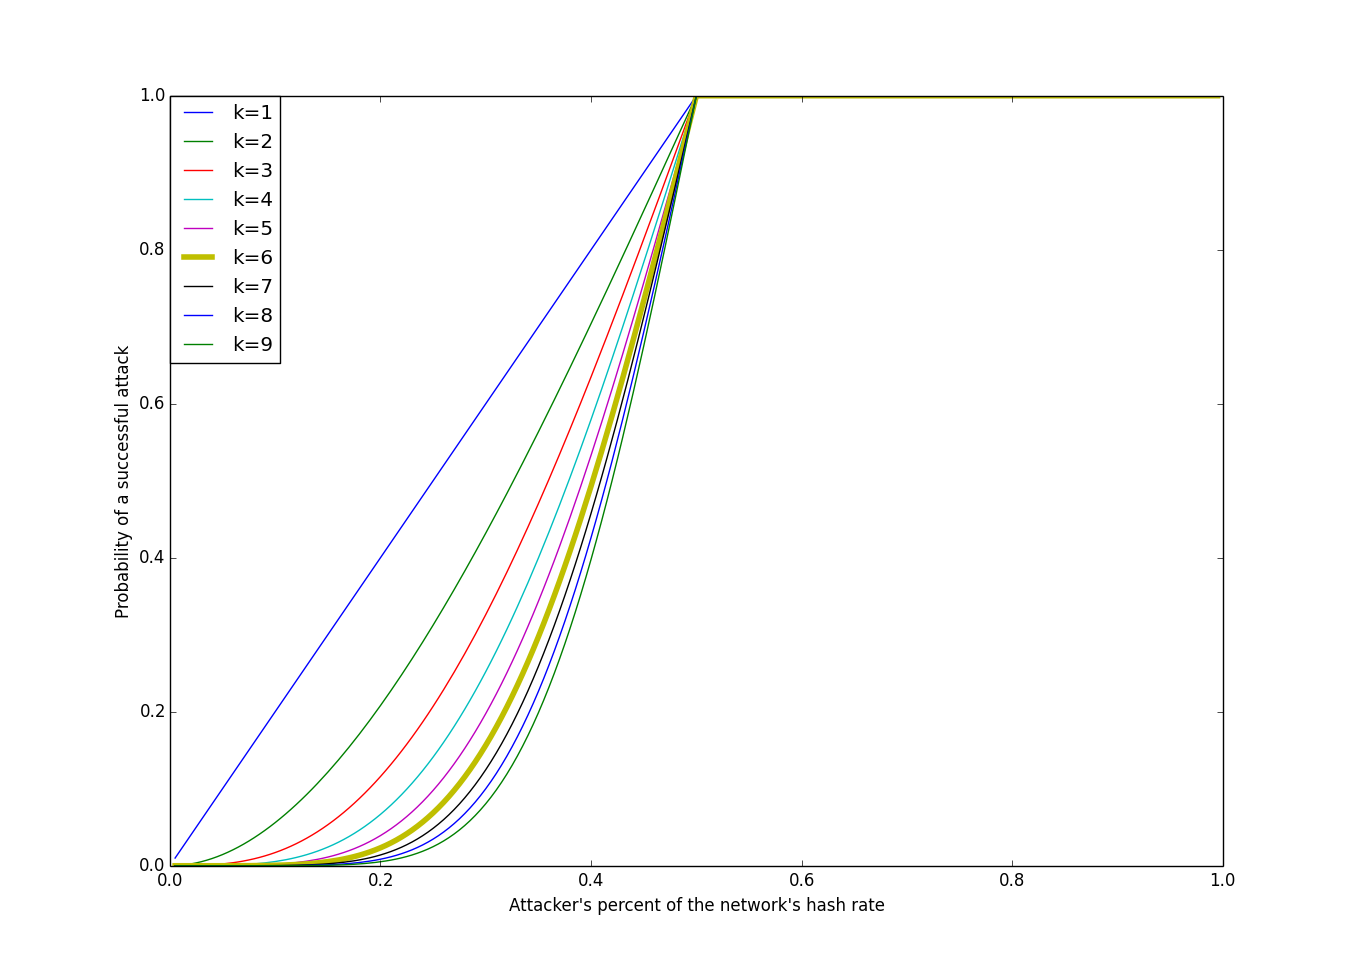
\includegraphics[width=\textwidth]{./images01/fig-bitcoin-attack.png}
\caption{Probability of a successful attack according to the network's hash rate of the attacker ($\beta$).\label{fig-bitcoin-attack}}
\end{figure}

%The number of blocks found in a given time interval $\Delta t$ is given by the Poisson distribution. So, the number of blocks found by the attackers $N_{\text{attacker}}$ follows a Poisson distribution with parameter $\lambda_{\text{attacker}} \Delta t = \frac{\beta \Delta t}{600}$, and the number of blocks found by the network $N_{\text{network}}$ follows a Poission distribution with parameter $\lambda_{\text{network}} \Delta t = \frac{\gamma \Delta t}{600}$. We would like to calculate $\mathbf{P}(N_{\text{attackers}} - N_{\text{network}} \geq k)$.

%$\mathbf{P}(Y_{n+k}^{\text{attacker}} < Y_{n}^{\text{network}})$


\section{Confirmation time and network capacity}
% Tempo na fila para confirmar transação

Let's say that when a new transaction is propagated it is enqueued in the unconfirmed transaction queue. Then, when a new block is found, some of these transactions in the queue are confirmed. We are interested in some measures of the queue, like the expected time to confirm a transaction and the queue's length.

Let's assume that all transactions have exactly the same size $S$ and pay exactly the same fee. If the Bitcoin block's maximum size is $M$, there would be room for $s = \lfloor M/S \rfloor$ transactions in each block. Using the results from \citet{bailey1954queueing}, we have found that $\pi_n = \frac{z_s-1}{z_s^{n+1}}$ is the probability of having $n$ unconfirmed transactions in the pool subjected to $s > m$, where $m=\frac{\lambda_{\text{TX}}}{\lambda_{\text{blocks}}}$ and $z_s$ is the single root of the polynomial $z^s(1+m(1-z))-1$ with $|z_s|>1$. The average size of the unconfirmed transaction pool is $\mathbf{E}(\pi) = \frac{1}{z_s - 1}$. Thus, $s > m \Rightarrow \lambda_{\text{TX}} < s \lambda_{\text{blocks}}$. The probabilities form a simple geometric series, and so they are exponentially decreasing. We may interpret it as a stable system, i.e., the unconfirmed transactions pool size is finite. In the Bitcoin's network, $\lambda_{\text{blocks}} = 1/\eta$ and the average number of transactions per block is $s=2,250$, so, this solution is valid when $\lambda_{\text{TX}} < 2,250/600 = 3.75$. Hence, $3.75$ is the maximum number of new transactions per second that the Bitcoin's network may handle. When $\lambda_{\text{TX}} > 3.75$, the unconfirmed transaction pool starts to grow indefinitely.

The average waiting time of a transaction to be confirmed, when $m < s$, is $\mathbf{E}(w) = \frac{1}{\lambda_{\text{TX}} (z_s-1)}$.

When $m \ll s$, $z_s \rightarrow 1 + 1/m$. So, the average number of unconfirmed transactions is $\mathbf{E}(\pi) \rightarrow m$ and the average waiting time $\mathbf{E}(w) \rightarrow \frac{1}{\lambda_{\text{blocks}}} = \eta = 600 \text{ seconds}$. In the Bitcoin's network, $s \gg m \Rightarrow \lambda_{\text{TX}} \ll 3.75$.

When $\lambda_{\text{TX}} \rightarrow s$, $z_s \rightarrow 1$. So, $\mathbf{E}(\pi) \rightarrow +\infty$.

Finally, we conclude that the Bitcoin's network capacity is $\lambda_{\text{blocks}} s = s/\eta = s/600$ transactions per second, where $s$ is the average number of transactions per block.


\section{Fork analysis}

% TODO BIP's and signaling bit --- see BIP 9 and BIP 135.

When a disagreement between miners' rules happens, that is referred as either a hard-fork or a soft-fork. It is said to be a soft-fork when the rules are backward compatible, and a hard-fork when the rules are not backward compatible. In general, a hard-fork relaxes the constraints, while the latter hardens them.

Suppose that the miners' are split in two groups, $G_1$ and $G_2$, with different rules. Let's say $H_1$ and $H_2$ are their hash rate, respectively. We have two different scenarios to analyze: (i) when neither of them accepts other's blocks; and (ii) when $G_2$ accepts $G_1$'s blocks, but not the other way around.

Scenario (i) is easy to analyze, because the network would just split and, after a while, both difficulties will be adjusted. Then, they will be just like two different Bitcoin networks.

Scenario (ii) is more trick. As $G_2$ accepts $G_1$ blocks, their hashrate will matter. If $H_1 > H_2$, then $G_2$ will frequently skip their blockchain, because $G_1$'s blockchain will be longer most of the time. If $H_1 < H_2$, then $G_2$ may have its own blockchain after a while --- a true fork. But what would happen if $H_1$ keeps increasing and eventually gets larger than $H_2$? It if happens for sufficient time, the whole $G_2$'s blockchain may be discarded in order to move to $G_1$'s blockchain when $G_1$'s gets longer.

\begin{theorem}
	When $H_1 > H_2$, the
\end{theorem}



%What would happen if, after a while, the groups agree again. How would the blockchain merge?



\chapter{Hathor's architecture}
% !TEX root = ../partial-blockchain.tex

This work introduces the Hathor's architecture, which lies between Bitcoin's and Iota's and may be a solution to scaling, centralization, and spam issues.

Like Iota, new transactions confirm previous ones, forming a Directed Acyclic Graph (DAG). For this, each transaction has its own proof-of-work which is solved by the issuer before propagating the transactions in the network. Like Bitcoin, miners find new ``blocks'' every 10 minutes in which they collect the fees and newly generated tokens. Each transaction has an ``accumulated weight'' which express the required effort to break the transaction, similar to Bitcoin's number of confirmations.

In Hathor, there are two difficulty levels: (i) one for new transactions which are just moving tokens around, and (ii) another one for ``blocks'' which are generating new tokens and collecting fees. The first may be adjusted to prevent spammers, which would spend too many resources to generate a great number of new transactions, whereas the latter is adjusted every 2,016 blocks to keep the pace of blocks on every 2 minutes.

Both miners and users will be working on proof-of-work, decentralizing even more the network's hash rate. Even though the users' difficulty is less than the miners', the hash rate will increase with every new user. The more transactions arrive, the higher the total hash rate. This may have good consequences in governance, which we will further discuss.

There is a trade-off about the \textit{difficulty} of new transactions. The higher it is, the harder it is to generate new transactions, preventing spammers but also making it harder for IoT devices generate new transactions. This difficulty may even be increased when a spam attack is in course and reduced when it is gone. If the difficulty is too high, IoT devices may sign their transactions and send them to another devices which have a greater hash rate and will solve their proof-of-work faster.

It also seems interesting to have this difficulty depending on new transaction's size (in bytes) and amount being moved. The idea here is to require more work when high amounts are at stake. It would not affect IoT devices, which are expected to usually move smaller amounts. Regarding the transaction's size, requiring more work for larger transactions may make sense because they may prevent abuses, such as a denial-of-service attack using enormous transactions which would consume a lot of node's bandwidth and disk space.

Another important security matter is that each transaction has to confirm all its inputs, i.e., there must be a confirmation path between all the transactions of the inputs and the transaction which are spending them. It is always possible since there is at least one confirmation path between any transaction and a tip. This ensures that, when a conflict is resolved, only the sub-DAG with root at the invalidated transaction will be affected. The remaining parts of the DAG remains the same.

The transactions are classified into three groups: (i) confirmed transactions, (ii) in-progress transactions, and (iii) unconfirmed transactions (tips). The confirmed transactions are the ones which have already been settled, i.e., their accumulated weights have reached a minimum level. The unconfirmed transactions (tips) are the brand new transactions which have not been confirmed even once yet, i.e., their accumulated weights are zero. The in-progress transactions are in the middle. They have already been confirmed a few times, but not enough to reach the minimum level required to be a confirmed transaction. For simplicity, the pending transactions encompass both in-progress and unconfirmed transactions.

Another transaction classification concerns its validation by the network. A transaction is said to be network validated if there are confirming paths from all tips to the transactions, i.e., the whole network has validated that the transaction is valid. It is important to notice that a transaction may be network validated but still pending, or even be confirmed but not network validated.

A \emph{block} is just a regular transaction with no inputs which confirms a previous block and at least two in-progress transactions or tips. There may be any number of outputs provided that they comply with the number of newly generated tokens. Each block collects all fees from all transactions confirmed by it which have not been confirmed by another block before. The blocks are ordered according to their timestamp. If two blocks have the same timestamp, the block hash is used as a tiebreaker.

In the low load scenario, there is a small number of new transactions coming into the network, which means they give a minor contribution to confirmations. In this case, the confirmation is held mostly by blocks. On the other hand, in the high load scenarios, there is a large number of new transactions giving a major contribution to confirmations. In this case, the blocks strengthen the confirmations, but many of them will have already been confirmed before the next blocks are found. The higher the number of new transactions, the faster the transactions are confirmed. The blocks assure a ``maximum confirmation time''.

The incentive scheme which keeps the network running is the same as Bitcoin's. Miners go towards fees and newly generate coins, whereas users just want to exchange their tokens. When there is no new transaction to be confirmed, the miners keep the network up and running while they find new blocks.


\section{Transaction confirmation}

Hathor uses similar concepts of weight and accumulated weight as Iota's. The weight depends only in the transaction itself, whereas the accumulated weight depends on its confirmations.

The weight of a transaction is calculated as $w = \log_2(k)$ where $k$ is the average number of hashes required to solve its proof-of-work.

The accumulated weight is the average number of hashes required to solve the proof-of-work of the transaction itself plus all the transactions which confirm it. Let $A$ be a transaction, its accumulated weight $w_A$ is calculated as $\log_2(2^{w_A} + \sum_{A \leadsto P} 2^{w_P})$.

In Bitcoin, it is well-known that one should wait at least ``six confirmations'' before accepting a transaction. This Bitcoin's criteria is based on some math presented in Satoshi's seminal work \citep{nakamoto2008bitcoin}. Adopting six confirmations is the same as demanding from attackers a minimal effort of six times the network's hash rate to successfully double spend those tokens. Let $H$ be the total hash rate of the network. Then, as $\mathbf{E}(Y_6) = 60 \text{ minutes}$, it will be necessary to calculate, on average, $\mathbf{E}(Y_6) \cdot H = 60 \cdot 60 \cdot H$ hashes to solve the proof-of-work of 6 blocks.

Therefore, in order to have the same level of security as Bitcoin, a transaction is said to be confirmed when its accumulated weight is greater than or equal to $\log_2(\mathbf{E}(Y_6) \cdot H) = \log_2(6 \cdot 128 \cdot H) = 7 + \log_2(6) + \log_2(H)$, where $H$ is calculated as the total hash rate of the miners plus the total hash rate of new transactions.


\section{Time between blocks}

The hash function used for the proof-of-work (PoW) is the same as Bitcoin: \emph{SHA-256} applied twice. Thus, most of the math analysis we have already done before is just the same.

Let $X$ be the number of trials to solve the PoW and $T$ be the time between blocks. We already know that $X$ follows a geometric distribution with $p = \frac{A}{2^{256}}$, where $A$ is inversely proportional to the difficulty, i.e., the smaller the $A$, the higher the difficulty. We also know that $T$ follows an exponential distribution with $\lambda = \frac{1}{\eta}$, where $\eta$ is the average time between blocks. As proved before, $\eta p H = 1$, thus let's define $w = \log_2(\mathbf{E}(X)) = \log_2(1/p) = \log_2(\eta H) = \log_2(\eta) + \log_2(H)$.

For the blocks, $\eta = 128$, thus, $\mathbf{E}(T) = 128 \text{ seconds}$, and $\mathbf{V}(T) = 16,384$. The symmetrical confidence interval with $\alpha = 10\%$ is $[6.56, 383.45]$, i.e., 90\% of the cases the distance between blocks will be between 6 seconds and just under 7 minutes.

Let $H$ be the hash rate of the miners, then, the weight of the blocks is calculated by

$$w_\text{blocks} = \log_2(128) + \log_2(H) = 7 + \log_2(H)$$

This weight will be updated every 2,016 blocks to take into consideration the change of $H$. First, $H$ will be estimated using the fact that $\mathbf{E}(Y_{2016}) = \frac{2016}{\lambda} = 2016 \eta = \frac{2016}{pH} = \frac{2016 \cdot 2^w}{H}$. Thus, $H = \frac{2016 \cdot 2^w}{\Delta t} \Rightarrow \log_2(H) = w + \log_2(2016) - \log_2(\Delta t)$, where $\Delta t$ is the time between the latest weight update and now. Finally,

$$w_\text{new} = 7 + w_\text{old} + \log_2(2016) - \log_2(\Delta t)$$

Notice that, if the hash rate has not changed, then $\Delta t = 128 \cdot 2016$ and $w_\text{new} = w_\text{old}$.


\section{Weight of the transactions}

There is a trade-off which must be considered in the weight of the transactions: the higher the weight, the better to prevent spam, but the worse to microtransactions. So, trying to fulfill both necessities, the weight will be a function of the transaction's size (in bytes) and total amount:

$$w_\text{tx} = \log_2(\text{size}) + \log_2(\text{amount}) + 0.5$$

Although the transaction size depends on the implementation, a typical transaction with 2 inputs and 2 outputs would have approximately 188 bytes. So, for instance, transfering 50,000 tokens would require a weight of 23, which means an average of $2^{23}$ trials to solve the proof-of-work.


\section{Issuance rate}

Hathor issues tokens every block, thus it is similar to Bitcoin. Even so, an important decision is whether it will issue a limited number of tokens or not. Bitcoin chose to issue a limited number of tokens. On the other hand, Ethereum and others chose to issue an ilimited number of tokens.

Both ways, the number of issued tokens is predictable. This feature itself brings confidence to the community, who will not face monetary intervention (unless they agree to) --- this comes in contrast with fiat money in which the central authority may change the monetary policy to adjust to political demands.

Bitcoin issuance rate started in 50 tokens per block and decreases over time. Every 210,000 blocks---4 years, on average---it halves the number of tokens issued per block. As Bitcoin smallest fraction is $10^{-8}$, after the 33th reduction it will stop issuing new tokens since $2^{33} > 50 \cdot 10^{-8}$. In total, the number of issued tokens will never exceed 21 million. For further information, see \cite{bitcoinsupply}.

%Using the same strategy, Hathor's issuance rate starts in 50,000 tokens per block and decreases over time. Different from Bitcoin, Hathor's tokens are always integers and cannot be split. Every 1,000,000 blocks, the number of tokens issued per block is halved. Thus, the supply is limited to 100 billion issued tokens during its whole life. To calculate the supply limit use the following equation:

%\begin{align*}
%    \sum_{k=0}^{\infty} 1,000,000 \cdot \left\lfloor \frac{50000}{2^k} \right\rfloor \approx
%    \sum_{k=0}^{\infty} 1,000,000 \cdot \frac{50000}{2^k} = 100 \text{ billion}
%\end{align*}

%As the average time between blocks is 128 seconds, it will take around 3 years, 9 months and 20 days between halves.


\section{Transaction fees}

In Bitcoin, the value of the fee is calculated as the difference between the transaction's outputs and the inputs. For instance, a transaction with inputs summing 8,000 and outputs summing 7,000 is paying 1,000 of fees.

In Hathor, each transaction may pay a fee to the next block which confirms it. But, even if the fee is zero, the miners are forced to confirm at least two pending transactions. These two pending transactions also confirm other transactions which may have no fees. In summary, transactions with no fees cannot be left behind and will always be confirmed by both blocks and other transactions.

One may arguee that it allows the whole network to never pay fees and they are right. In the beginning, miners' incentive is driven by new tokens instead of fees. In the long term, it may be necessary to require a minimum fee to keep the miners working, depending on the chosen issuance policy.


\section{Transaction validation}

A transaction will be considered valid when it complies with the following rules: (i) it spends only unspent outputs; (ii) the sum of the inputs is greater than or equal to the sum of the outputs; (iii) the number of inputs is at most 256; (iv) the number of outputs is at most 256; (v) it confirms at least two pending transactions; (vi) it solves the proof-of-work with the correct weight.

The transaction has a timestamp field which is used to record when the transaction was generated. This timestamp field must be in UTC time to prevent timezone issues. It must also be within at most 5 minutes from the current time, otherwise the transaction will be discarded.

The digital signature is used to ensure that only the owners may spend their tokens. It will be calculated signing the transaction's input and output only. This allows the transaction to be signed in one device and to be sent to another device that will choose which transaction will be confirmed and will solve the proof-of-work.

Services of solving proof-of-work may also be offered by companies. They give their customers a wallet address and they send the payment inside of the transaction itself. This allows IoT devices to save energy, delegating the task of solving the proof-of-work.

In case of transaction conflict, in which two transactions try to spend the same tokens, the one with higher accumulated weight is chosen and the other is invalidated. Although it is not a possible policy in Iota because of the submarine attack, Hathor does not have the same problem. In Hathor, like in Bitcoin, the submarine attack is only possible if the attacker has a hash rate higher than the whole network, including the miners. In other words, when analysing the double spending attack, Hathor is as safe as Bitcoin.


\section{Orphan blocks}

Different from Bitcoin, there is no orphan blocks in Hathor. Unless a block confirms either directly or indirectly an invalid transaction, every block is valid. There is no need to left a block behind since its proof-of-work is increasing transactions' accumulated weight.

If two blocks are trying to collect fees from the same transactions, the one with higher timestamp will be discarded.


\section{Governance}

In general, cryptocurrencies are decentralized, which means there is no central authority who decides its future, i.e., no one can enforce their will. Every decision must be accepted by its community, which means the community must agree. But what happens if they do not agree? When a consensus is not reached, the rules remain the same and the cryptocurrency may stall. The lack of a central authority may generate long debates, split the community, slow down strategic decision-making, and, ultimately, come to a ``civil war''---it is precisely what happened between Bitcoin Core (BTC) and Bitcoin Cash (BCH) in 2017 \citep{bloomberg2017civilwar, forbes2017civilwar}.

Governance is an important part of a cryptocurrency because it must evolve, which means its community must agree into changing the rules. Governance is an agreement of how the community will proceed to change the rules.

Despite the large literature available about governance, what separates Blockchain-based cryptocurrencies from them is the decentralization (against the hierarchical model). The number of papers about governance in decentralized cryptocurrencies has been growing, but it still lacks a solution. \citet{hacker2017corporate} resorts to the theory of complex systems and proposes a governance framework for decentralized cryptocurrencies, which is, in summary, a centralized coordination entity. \citet{hsieh2017internal} has analyzed the effects of governance in returns using panel data on several cryptocurrencies. They present a deeper discussion about the parts of a governance mechanism and concludes that

\begin{quote}
``... on the one hand, investors value cryptocurrencies’ core value proposition, rooted in decentralization; but on the other hand, are suspicious of decentralized governance at higher levels in the organization because they could slow down strategic decision-making (e.g., regarding the introduction of new innovations) or create information asymmetries between investors and technologists.''
\end{quote}

I believe that the solution to a good governance will come from financial incentives to all players to find a common ground. In Bitcoin, users have less bargaining power than miners because they do not contribute with work, whereas, in Hathor, both miners and users are working together. So, when it comes to changing the rules, the bargaining power is more distributed than in Bitcoin. The distribution depends on the ratio of the miners' hashpower and the users' hashpower. The higher the ratio, the closer to Bitcoin's governance. The lower the ratio, the higher the bargaining power of the users.

%- Punishment for miners/transactions which does not comply with the rules.
%- Rule change policy.

\section{Expected number of tips}

It is intuitive that the number of tips depends on the number of transactions per second. The higher the number of transactions per second, the higher the number of tips. We can model the number of tips at time $t$ as a stochastic process, which means it changes over time following some probability distribution. Stochastic processes have two important states: transient and steady. A process is in transient state when its properties are changing over time, whereas it is in steady state when its properties has already converged.

Let's assume that the number of transactions per second is constant and does not change over time. Thus, at the beginning, there will be no tips, and the number will increase until it converges to its stable quantity. The process is in transient state until it reaches stability. Then, it is in the steady state. Notice that the number of tips also change in steady state, but its average does not. It just floats around the average.

If the number of transactions per second increases, the process returns to the transient state and moves towards the new steady state. In practice, the number of transactions per second is always changing, so is the steady state.

\citet{tangle2016} has modeled the stochatic process of the total number of tips. It proves that the average number of tips, in the steady state, is:

$$\frac{\lambda_\text{TX} \cdot 2^{w_\text{TX}}}{\log(2)H}$$

A simple idea to get to this equation is through flow analysis: In steady state, we may say that the number of new tips must equal the number of tips being confirmed in a given time window. Thus, in order to estimate the number of tips in the steady state, let's consider the process in which the rate of inward tips is $\lambda_\text{TX}$, whereas the rate of outward tips is $\rho$.

Let $K$ be the number of tips at a given time. Thus, after $\Delta t$ seconds, $\Delta \text{tips} = \lambda_\text{TX} \Delta t - \rho K \Delta t$. In the steady state, $\Delta \text{tips} = 0$, hence $K = \frac{\lambda_\text{TX}}{\rho}$.

The rate of outward tips is proportional to the rate in which devices solve the proof-of-work of transactions. Let $H$ be the devices' hash rate, then, $\rho = \alpha \cdot H \cdot 2^{-w_\text{TX}}$, where $\alpha$ is the coefficient of proportionality.

Finally,

$$K = \frac{\lambda_\text{TX}}{\alpha} \frac{2^{w_\text{TX}}}{H}$$

If new transactions would always confirm two tips, then $\alpha$ would equal 2. But, it may confirm one or even zero tips because concurrent new transactions may confirm their tips first. Thus, $0 < \alpha \le 2$. According to the equation found in \citet{tangle2016}, $\alpha = \log(2) = 0.693147$.

%$$\frac{\lambda_\text{TX} \cdot 2^{w_\text{TX}}}{2H} \le K \le \frac{\lambda_\text{TX} \cdot 2^{w_\text{TX}}}{H}$$

%\section{Attacks \& Conflicting transactions}
%\section{Scripts \& Contracts}
%\section{Bandwidth consumption}



\chapter{Methodology}

The methodology we have used is computer simulation. Through the simulation of many scenarios of Hathor, we will understand how the network behaves in complex scenarios, including when the load suddenly increases, and when the network is under attack.

The simulator has been developed using an event-based design which is capable of running hours of simulation in just a few minutes. It creates agents who decide to make a transaction, then they select which transactions will be confirmed, next they spend some time working in the proof-of-work, and, finally, they propagate the transaction to the network. The other agents receive the transaction and may accept or deny it. The agents may use different parameters among themselves.

When a new transaction emerges, it chooses two tips to confirm before solving the proof-of-work. When it finishes solving the proof-of-work, the transaction is propagated and becomes a tip. So, two new transactions may choose the same tips to confirm. If there are $t$ tips, a new transaction will randomly choose 2 out of these $t$ tips, even if they have already been chosen by other new transactions --- in fact, they do not know which have been chosen because these new transactions have not been propagated yet.

When a new transaction is added to the Hathor's network, it uses a depth-first search \citep{cormen2009introduction} to update the aggregated weight of the directly and indirectly confirmed transactions. The depth-first search is interrupted when it reaches a transaction which the accumulated weight is larger than a given threshold. This interruption significantly increases the overall performance of the simulation. If the accumulated weight of the whole DAG is an important metric, the whole DAG may be updated in specific times to get a measurement (instead of every new transaction).

%, (ii) to calculate its own score, and (iii) to generate a topological sort \citep{cormen2009introduction}. The topological sort is used to calculate the longest path from all other transactions to the new transaction, and this longest path is used to update the depth of the whole DAG. If the new transaction confirms only transactions which has already been confirmed, the depth update is skipped thanks to Theorem \ref{theorem-new-tx-not-tip}.

Simulator's random variables simulator are all sampled from their distributions. The time between two transactions is sampled from an exponential distribution with $\lambda_\text{TX}$. The number of attempts to find a solution of the proof-of-work is sampled from a geometric distribution with $p=2^{w}$, where $w$ can be either $w_\text{TX}$ or $w_\text{block}$. The amount of time spent to solve the proof-of-work is calculated dividing the number of attempts by the hash rate of the device (which could be either a miner or an user). The time between blocks is just the amount of time spent to solve the proof-of-work with $w_\text{block}$.

Transactions (and blocks) do not have inputs, outputs, and scripts. They have only pointers to other transactions, which form the DAG. They also store their weight, accumulated weight, timestamp, and some statistics used for reports.

New miners or users may be added or removed any time during a simulation. This allows the simulation of many different scenarios, such as increasing the number of miners, a sudden increase in the number of transactions per second, a sudden decrease in the number of miners, and so forth.

It is also possible to create metrics, which sample a statistic every $\Delta t$ seconds. There are two metrics available: (i) TipsMetric, which stores the number of tips at a given simulation time, and (ii) UtterlyAcceptanceMetric, which finds the new utterly accepted transactions and store how long it took.

To find the network validated transactions, I run a breadth-first search (bfs) for each tip. Transactions visited in all searches are being confirmed by all tips and, by definition, are network validated transactions.

%The simulator will output different reports: (i) snapshots of the DAG at interesting moments, such as Fig. \ref{fig-tangle-example}, \ref{fig-tangle-swarm}, and \ref{fig-tangle-conflict}; (ii) histogram of confirmation time, such as Fig. \ref{fig-tangle-hist} and \ref{fig-tangle-hist-2}; and many others.


\chapter{Analysis of Hathor}

% TODO Include the parameters of the simulations.

Hathor's architecture lies between Iota and Bitcoin's architectures. It is similar to Bitcoin's architecture when the number of transactions per second is low, while it is similar to Iota's architecture when the number of transactions per second is high. There is no ``switching'' between Bitcoin and Iota. It just behaves like one or another according to the network. In order to check this statement, I have performed some simulations.

First, two simulations in the extreme cases: (i) no miners, (ii) no transactions. The first should have precisely the same behavior as Bitcoin's blocks with one block after the other forming a long chain. The latter should have a similar behavior as Iota's, forming a Direct Acyclic Graph (DAG) with new transactions confirming previous ones. We can see in Figure \ref{fig:hathor-similarities} that both cases seem to be correct.

Next, I have run a more realistic simulation, with both miners and transactions. As we can see in Figure \ref{fig:hathor-dag}, Hathor's structure is a mix of Iota and Bitcoin's structure. The transactions are forming a DAG while, in parallel, the blocks are forming a chain inside the DAG.

\begin{figure}[!htb]
\centering
\subfloat[No miners]{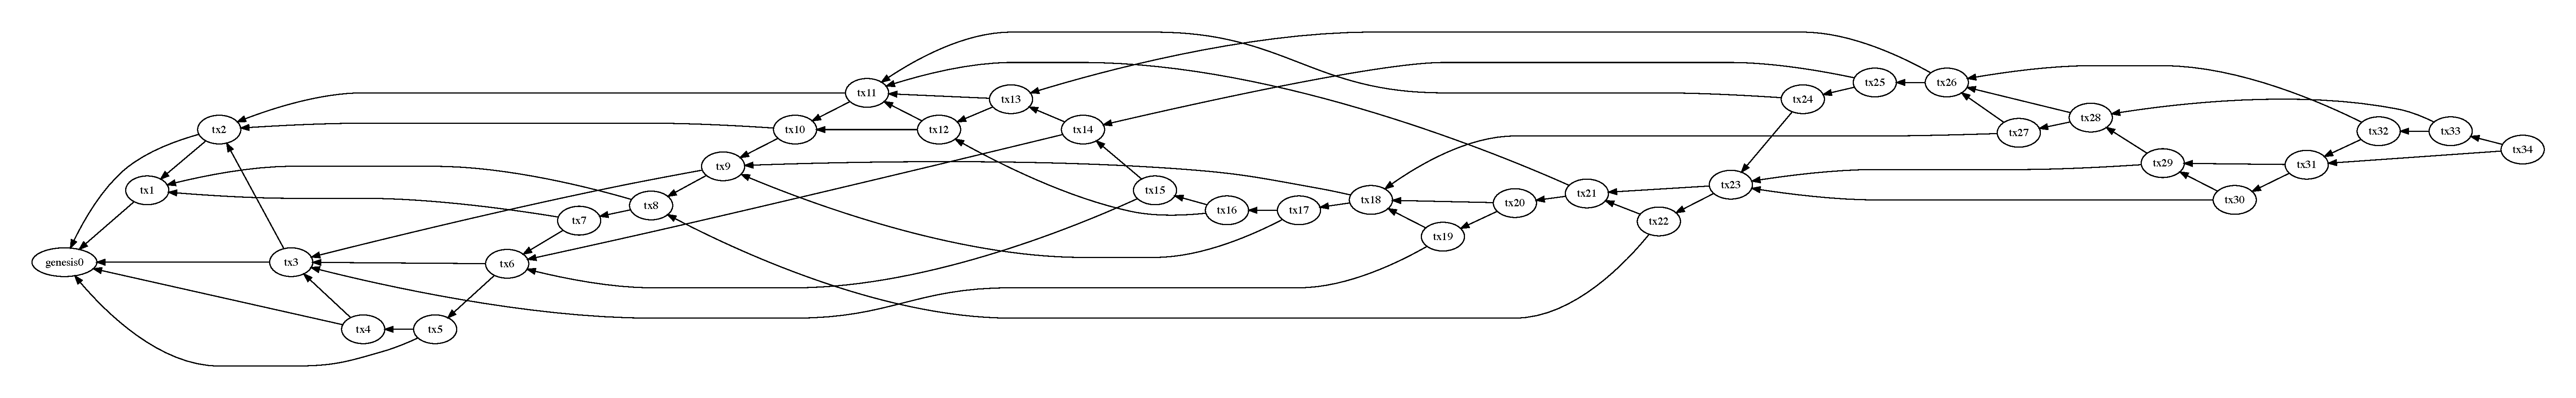
\includegraphics[width=0.5\textwidth]{./images01/sim/no_miners.pdf}}
\subfloat[No transactions]{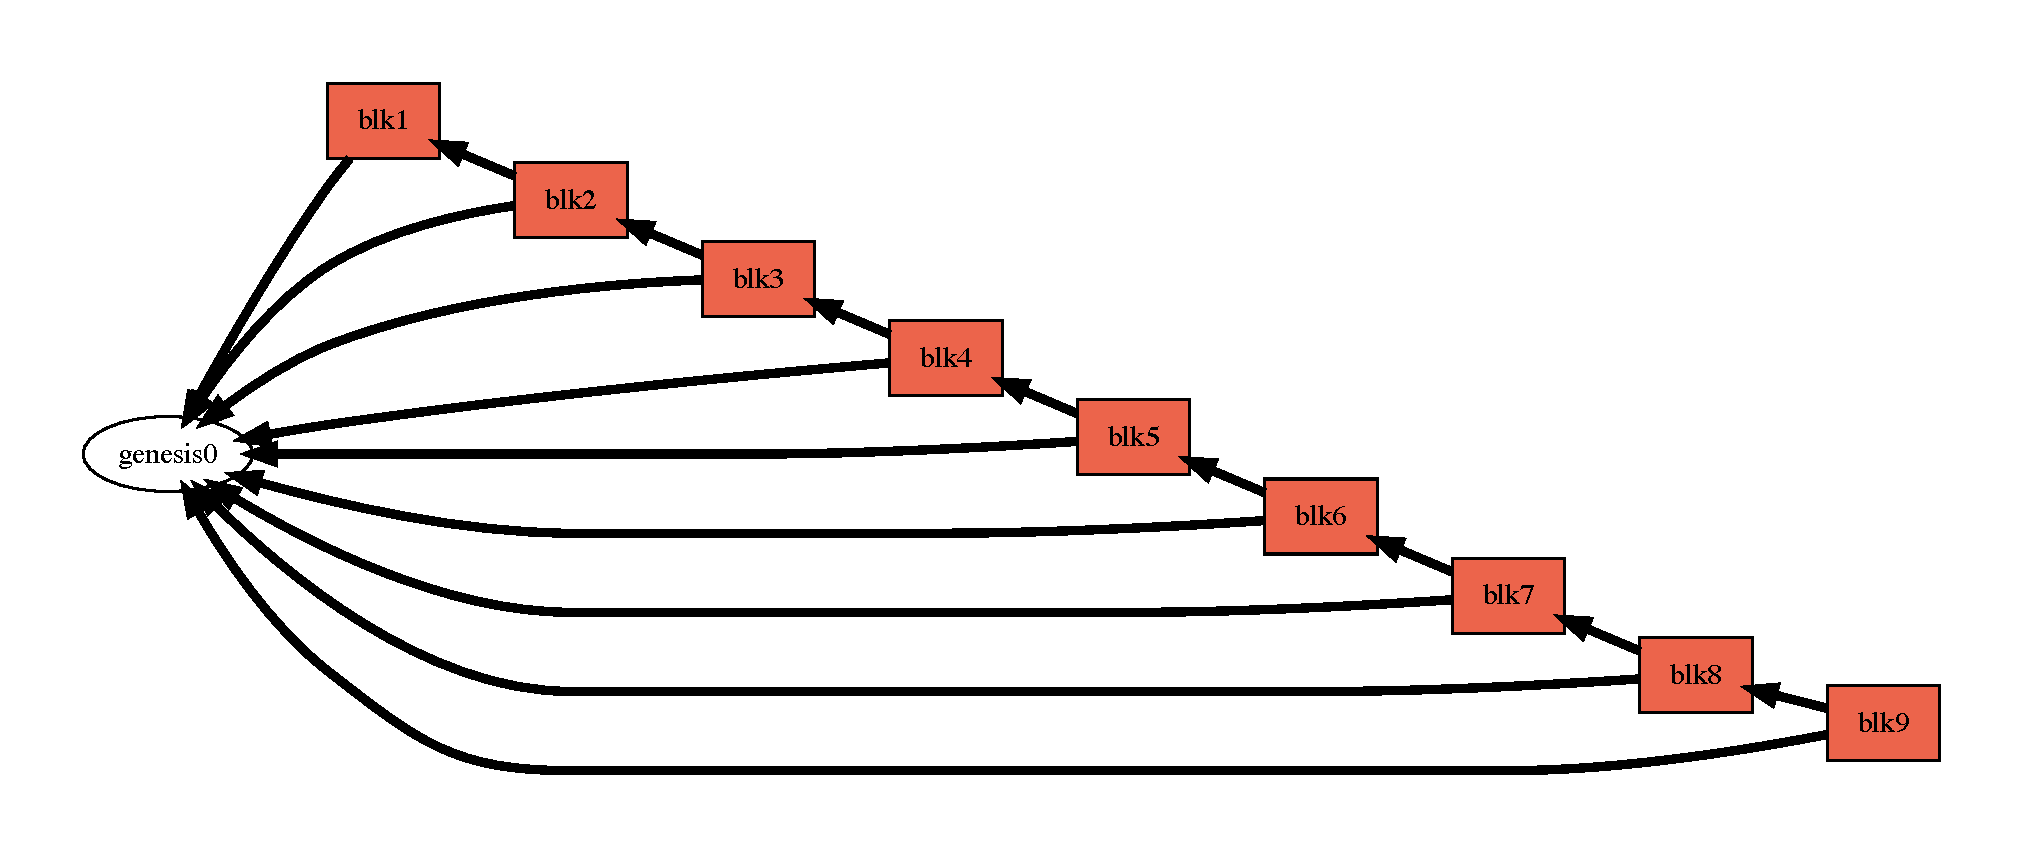
\includegraphics[width=0.5\textwidth]{./images01/sim/only_miners.pdf}}
\caption{Visualization of a Hathor's graph in two particular cases: (a) no miners, (b) no transactions. It shows that when there are no miners, Hathor is similar to Iota (same structure, but different parameters), and when there is no transactions, it is similar to Bitcoin.\label{fig:hathor-similarities}}
\end{figure}

\begin{figure}[!htb]
\centering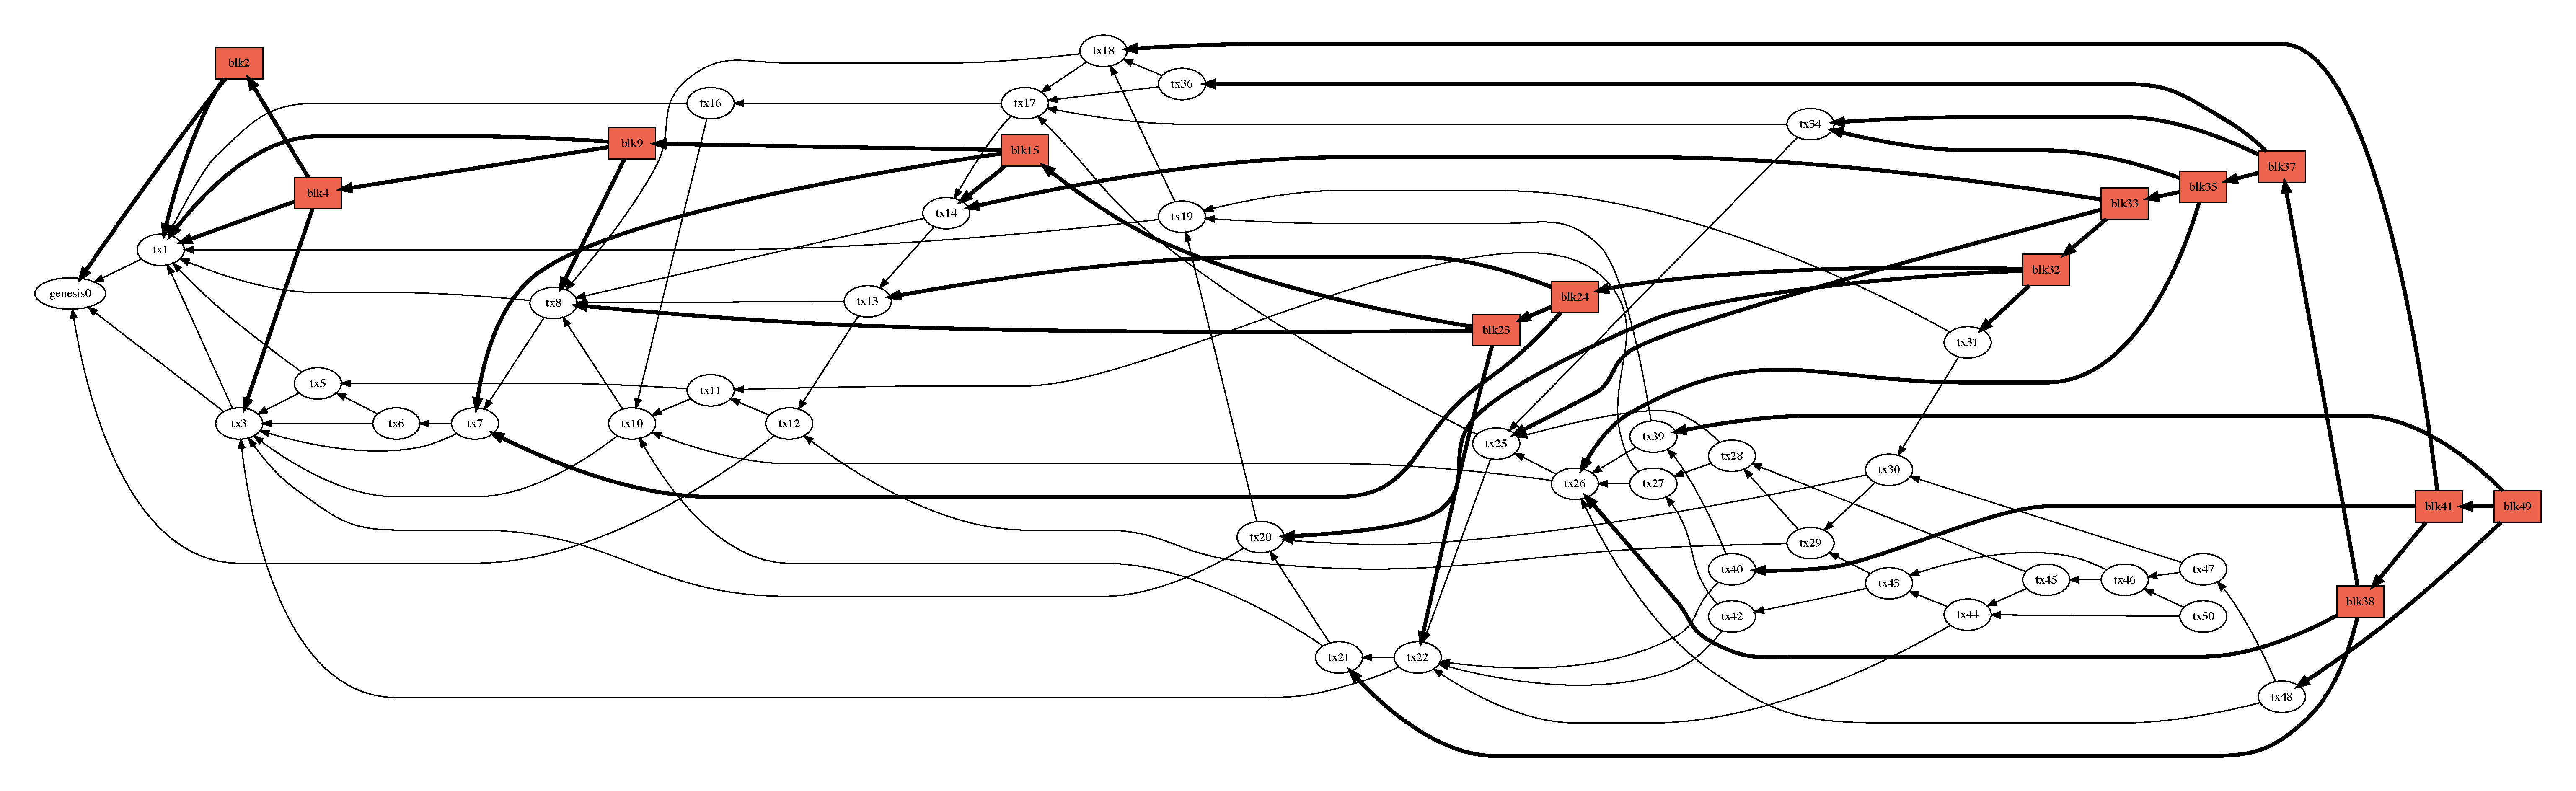
\includegraphics[width=\textwidth]{./images01/sim/hathor.pdf}
\caption{Visualization of a Hathor's graph with transactions and blocks. Red boxes are blocks, and white circles are simple transactions. The arrows show the confirmations.\label{fig:hathor-dag}}
\end{figure}


\section{Confirmation time}

Another evidence that Hathor lies between Iota and Bitcoin is found when comparing the time to confirm a transaction. In this context, a transaction is said to be confirmed when it has reached an accumulated weight similar to six times the hash rate of the whole network (miners and new transactions). This criteria is equivalent to the well-known ``6 confirmations'' of Bitcoin, which is adopted by almost the whole ecosystem.

Thus, I have run a simulation in which miners are majority and there are few transactions. In Figure \ref{fig:hathor-tct-low-mid}, we may see a good fit between the confirmation time of a transaction and the theoretical distribution of the time to find six blocks in Bitcoin (which is $Y_6$ and follows an Erlang distribution). The blocks create ``maximum confirmation time'', since they are found with a precise pace, i.e., when there is not enough new transactions coming, the confirmation is done by the blocks. But, when the load is increased, Hathor's confirmation time is reduced and diverges from Bitcoin's time distribution. The reasoning is that confirmations coming from other transactions start to play an important role and accelerates the speed of confirmations, i.e., there is no need to wait for the next blocks, because the transactions are confirming themselves. This is what allows Hathor to scale and support higher volumes, indeed.

\begin{figure}[!htb]
\centering
\subfloat[Low load]{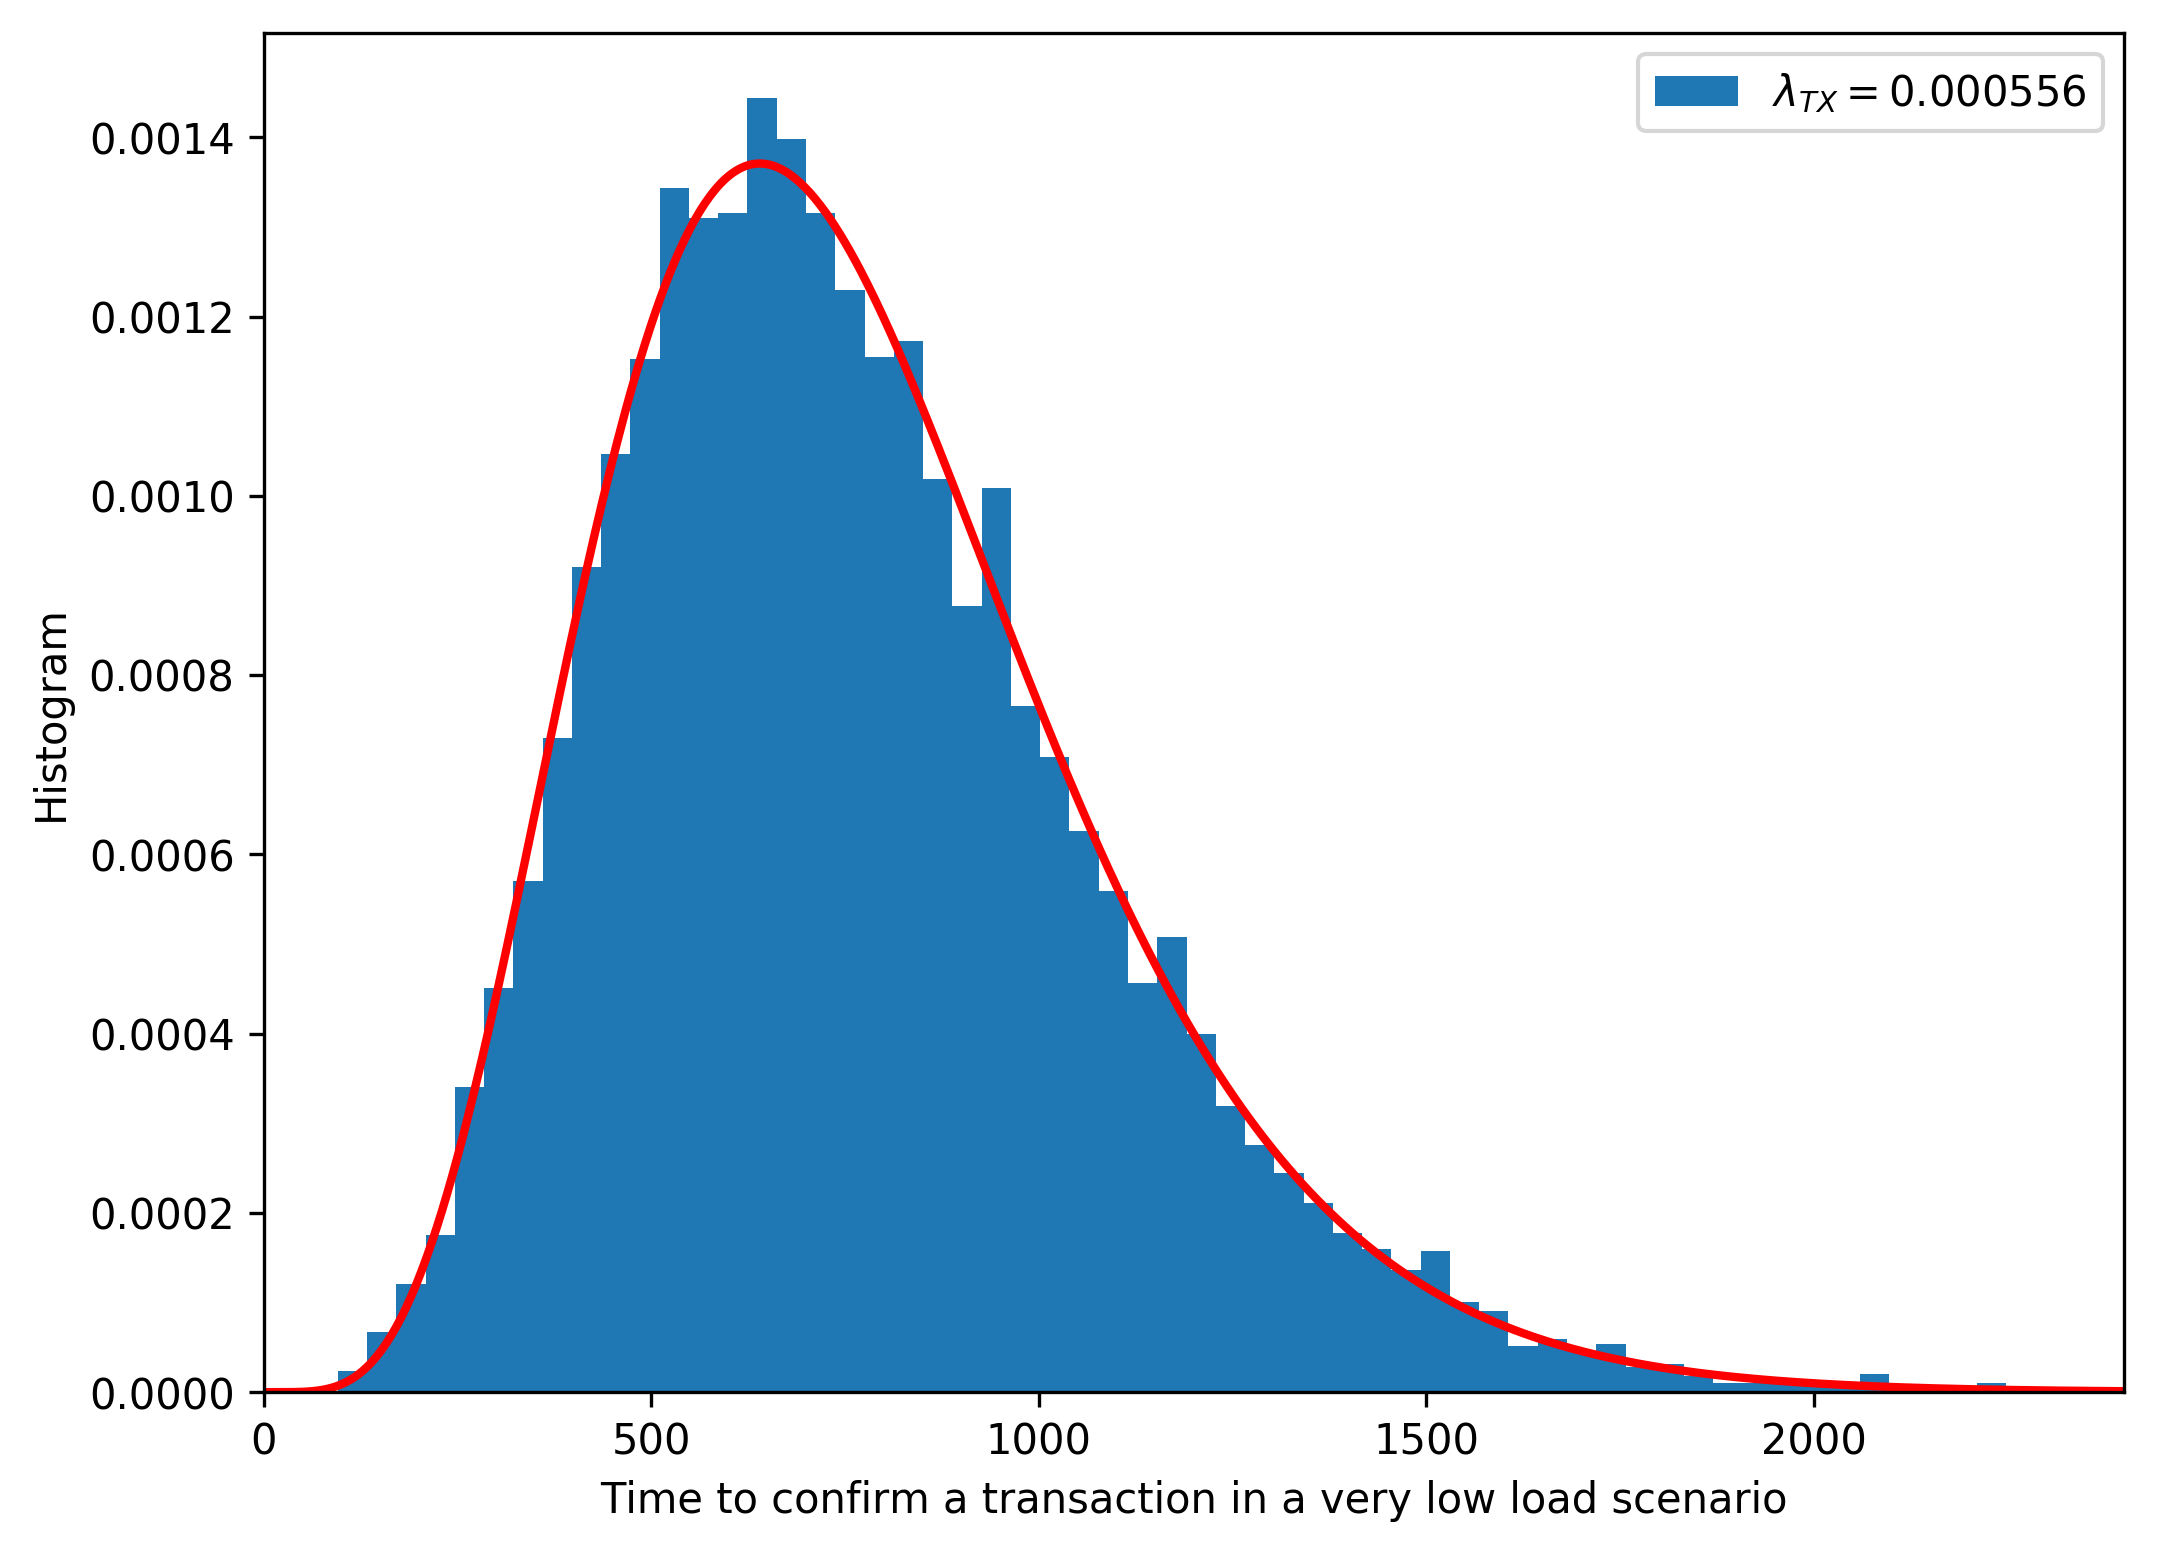
\includegraphics[width=0.5\textwidth]{./images01/sim/tct-low-load.png}}
\subfloat[Mid load \label{fig:hathor-tct-mid-load}]{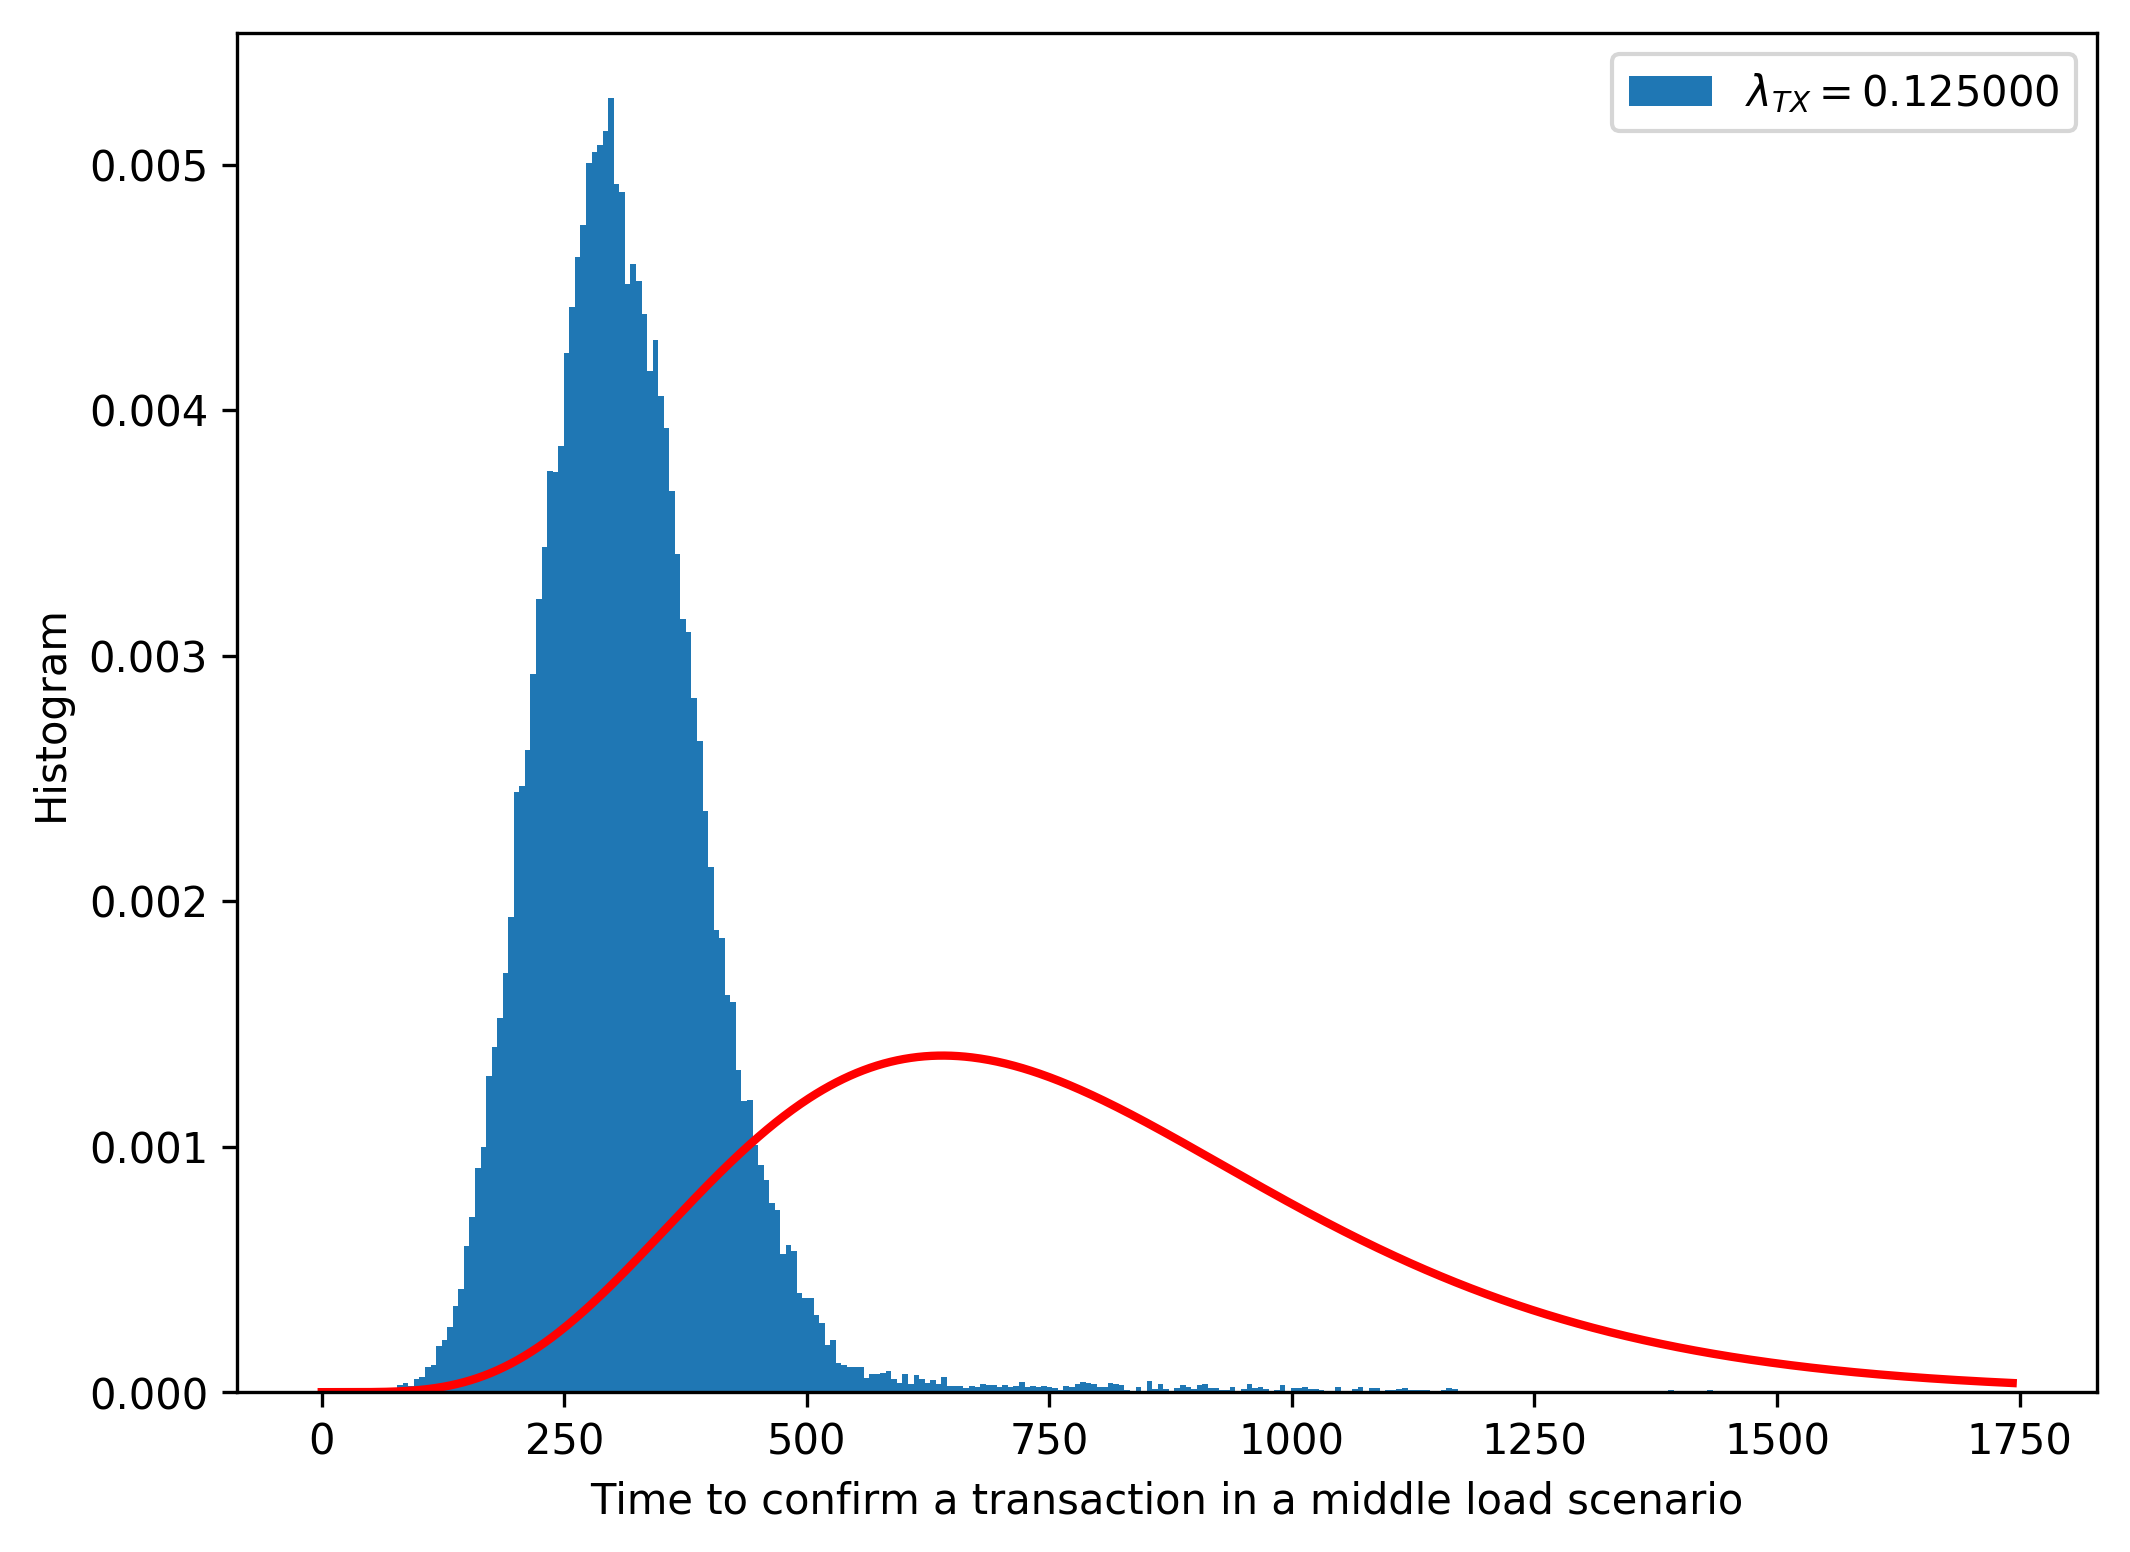
\includegraphics[width=0.5\textwidth]{./images01/sim/tct-mid-load.png}}

\caption{Confirmation time in two scenarios: (a) low load, (b) mid load. The red curve is the distribuion of the time to find six blocks in Bitcoin (which follows an Erlang distribution). As we can notice, in the low load scenario, Hathor's confirmation time behaves just like Bitcoin's. When the load is increased, it starts to diverge from Bitcoin's distribution. \label{fig:hathor-tct-low-mid}}
\end{figure}

We may see Hathor's confirmation time moving from Bitcoin's to Iota's in Figure \ref{fig:hathor-tct-many}. Notice that the confirmation timer is getting smaller as the number of transactions per second increases. Figure \ref{fig:hathor-tct-many-right} is a zoom-in in the right side, and we can see again the good fit between Hathor Bitcoin's confirmation time under low load.

\begin{figure}[!htb]
\centering
\subfloat[The whole picture]{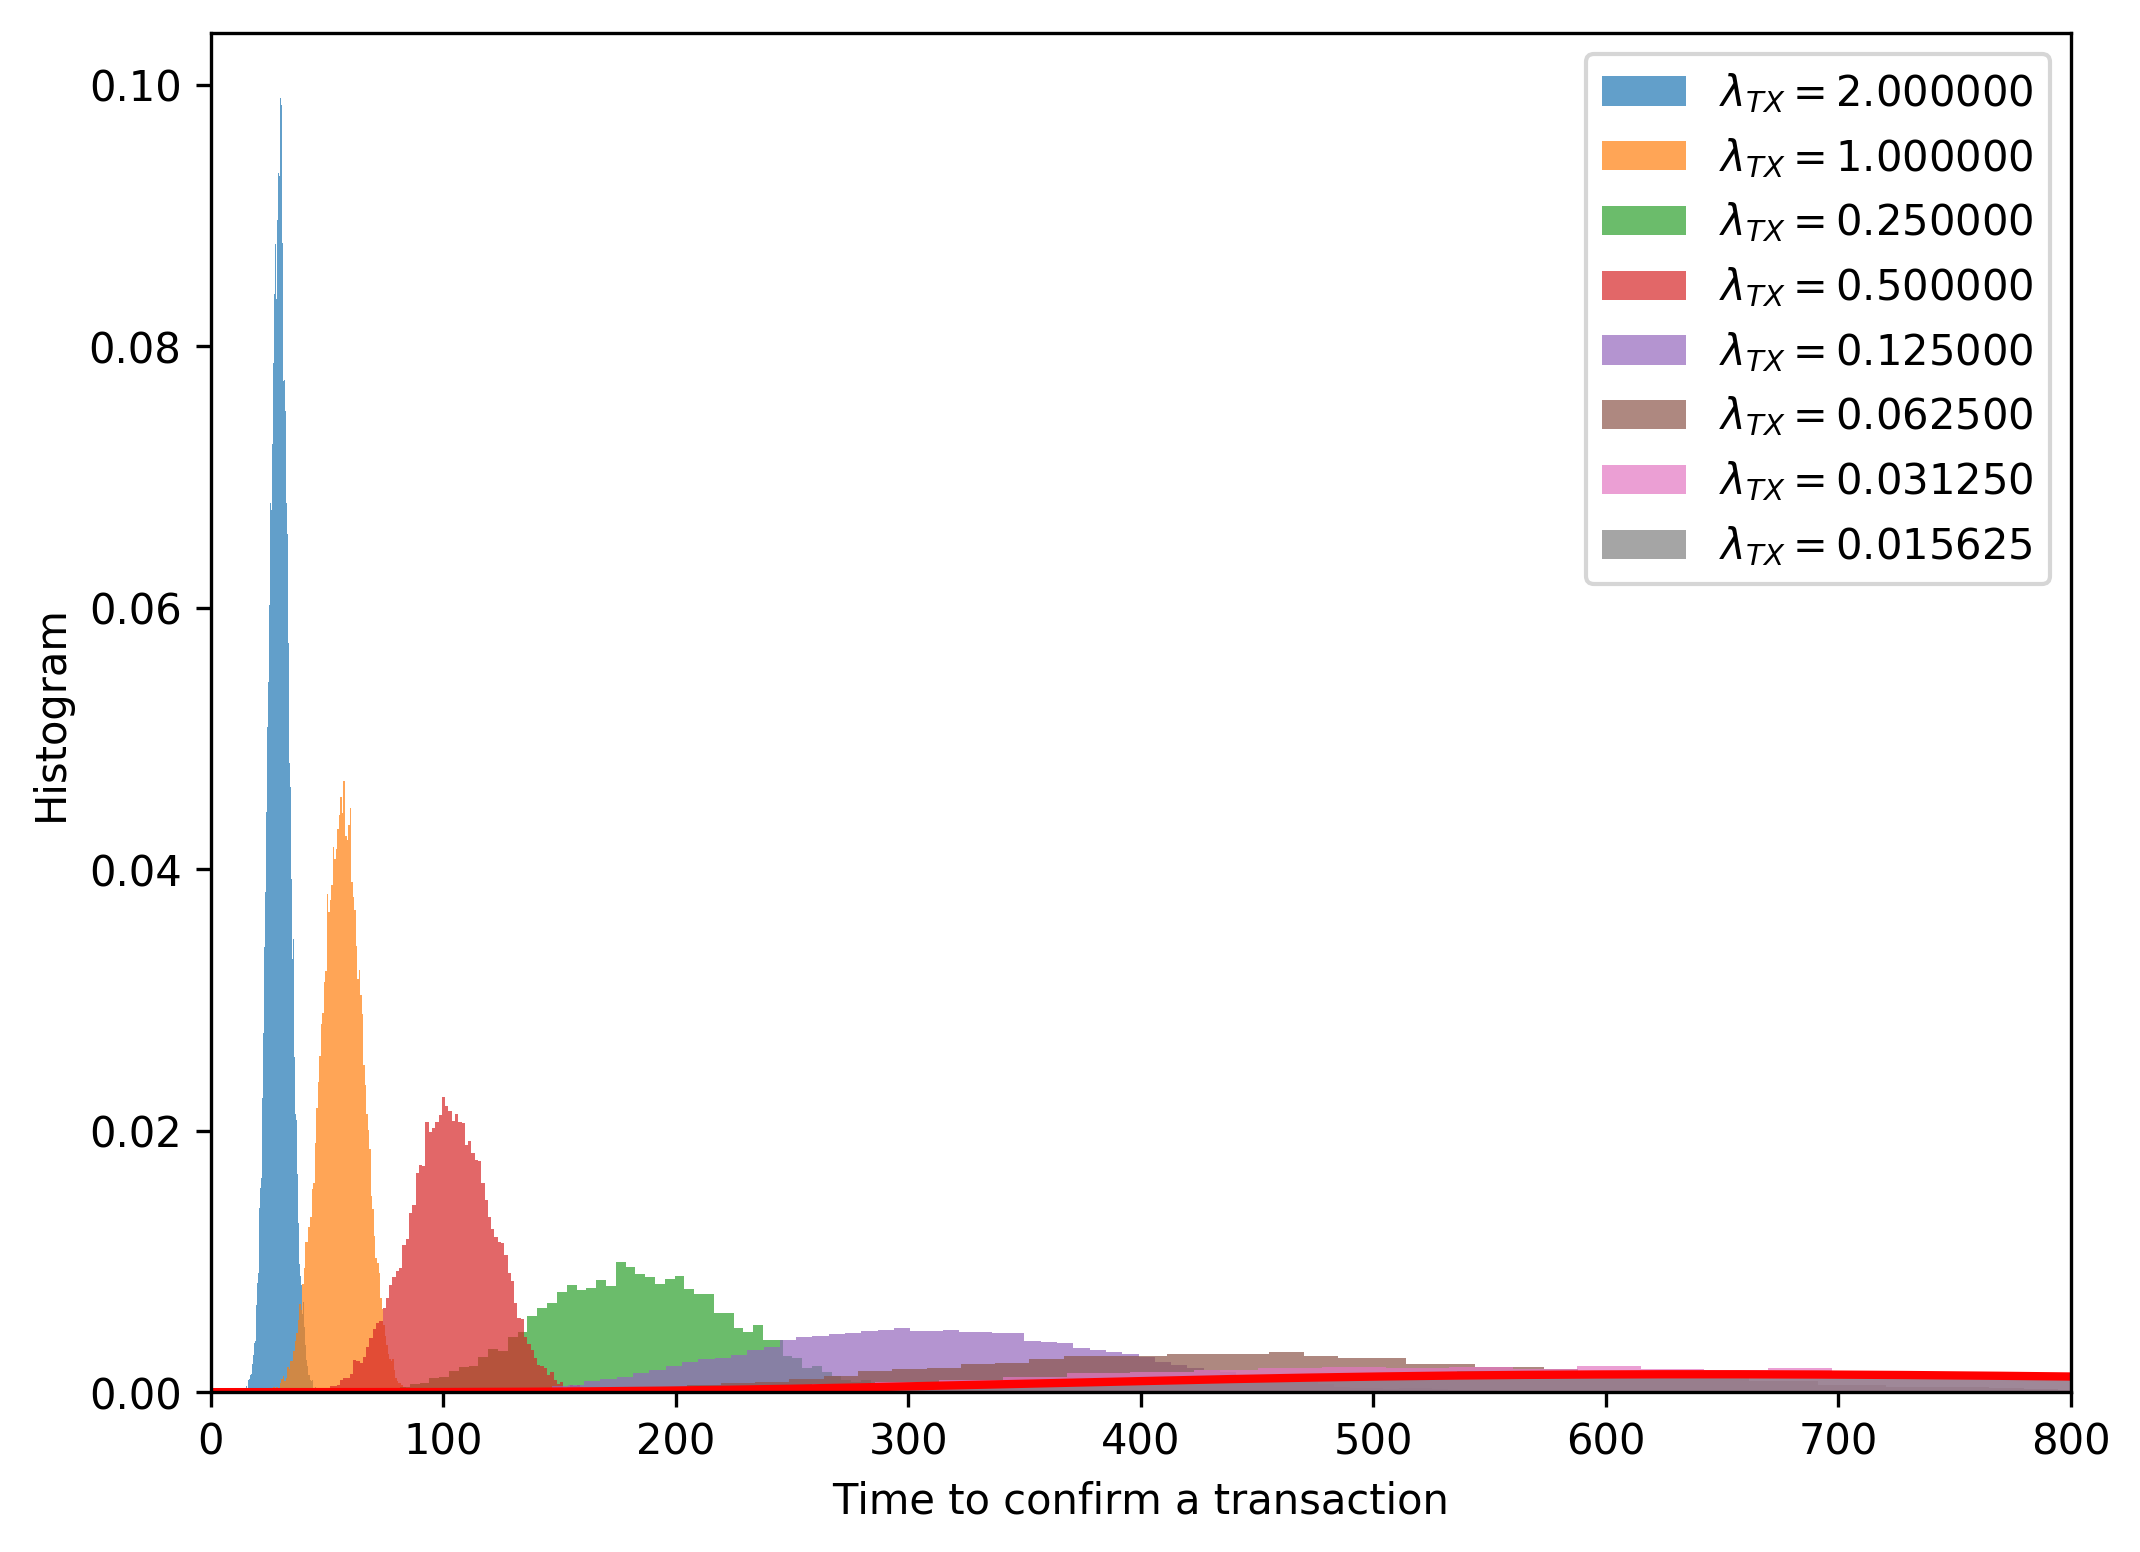
\includegraphics[width=\textwidth]{./images01/sim/tct-many-loads-2.png}}

\subfloat[Zoom in the left part of the above chart]{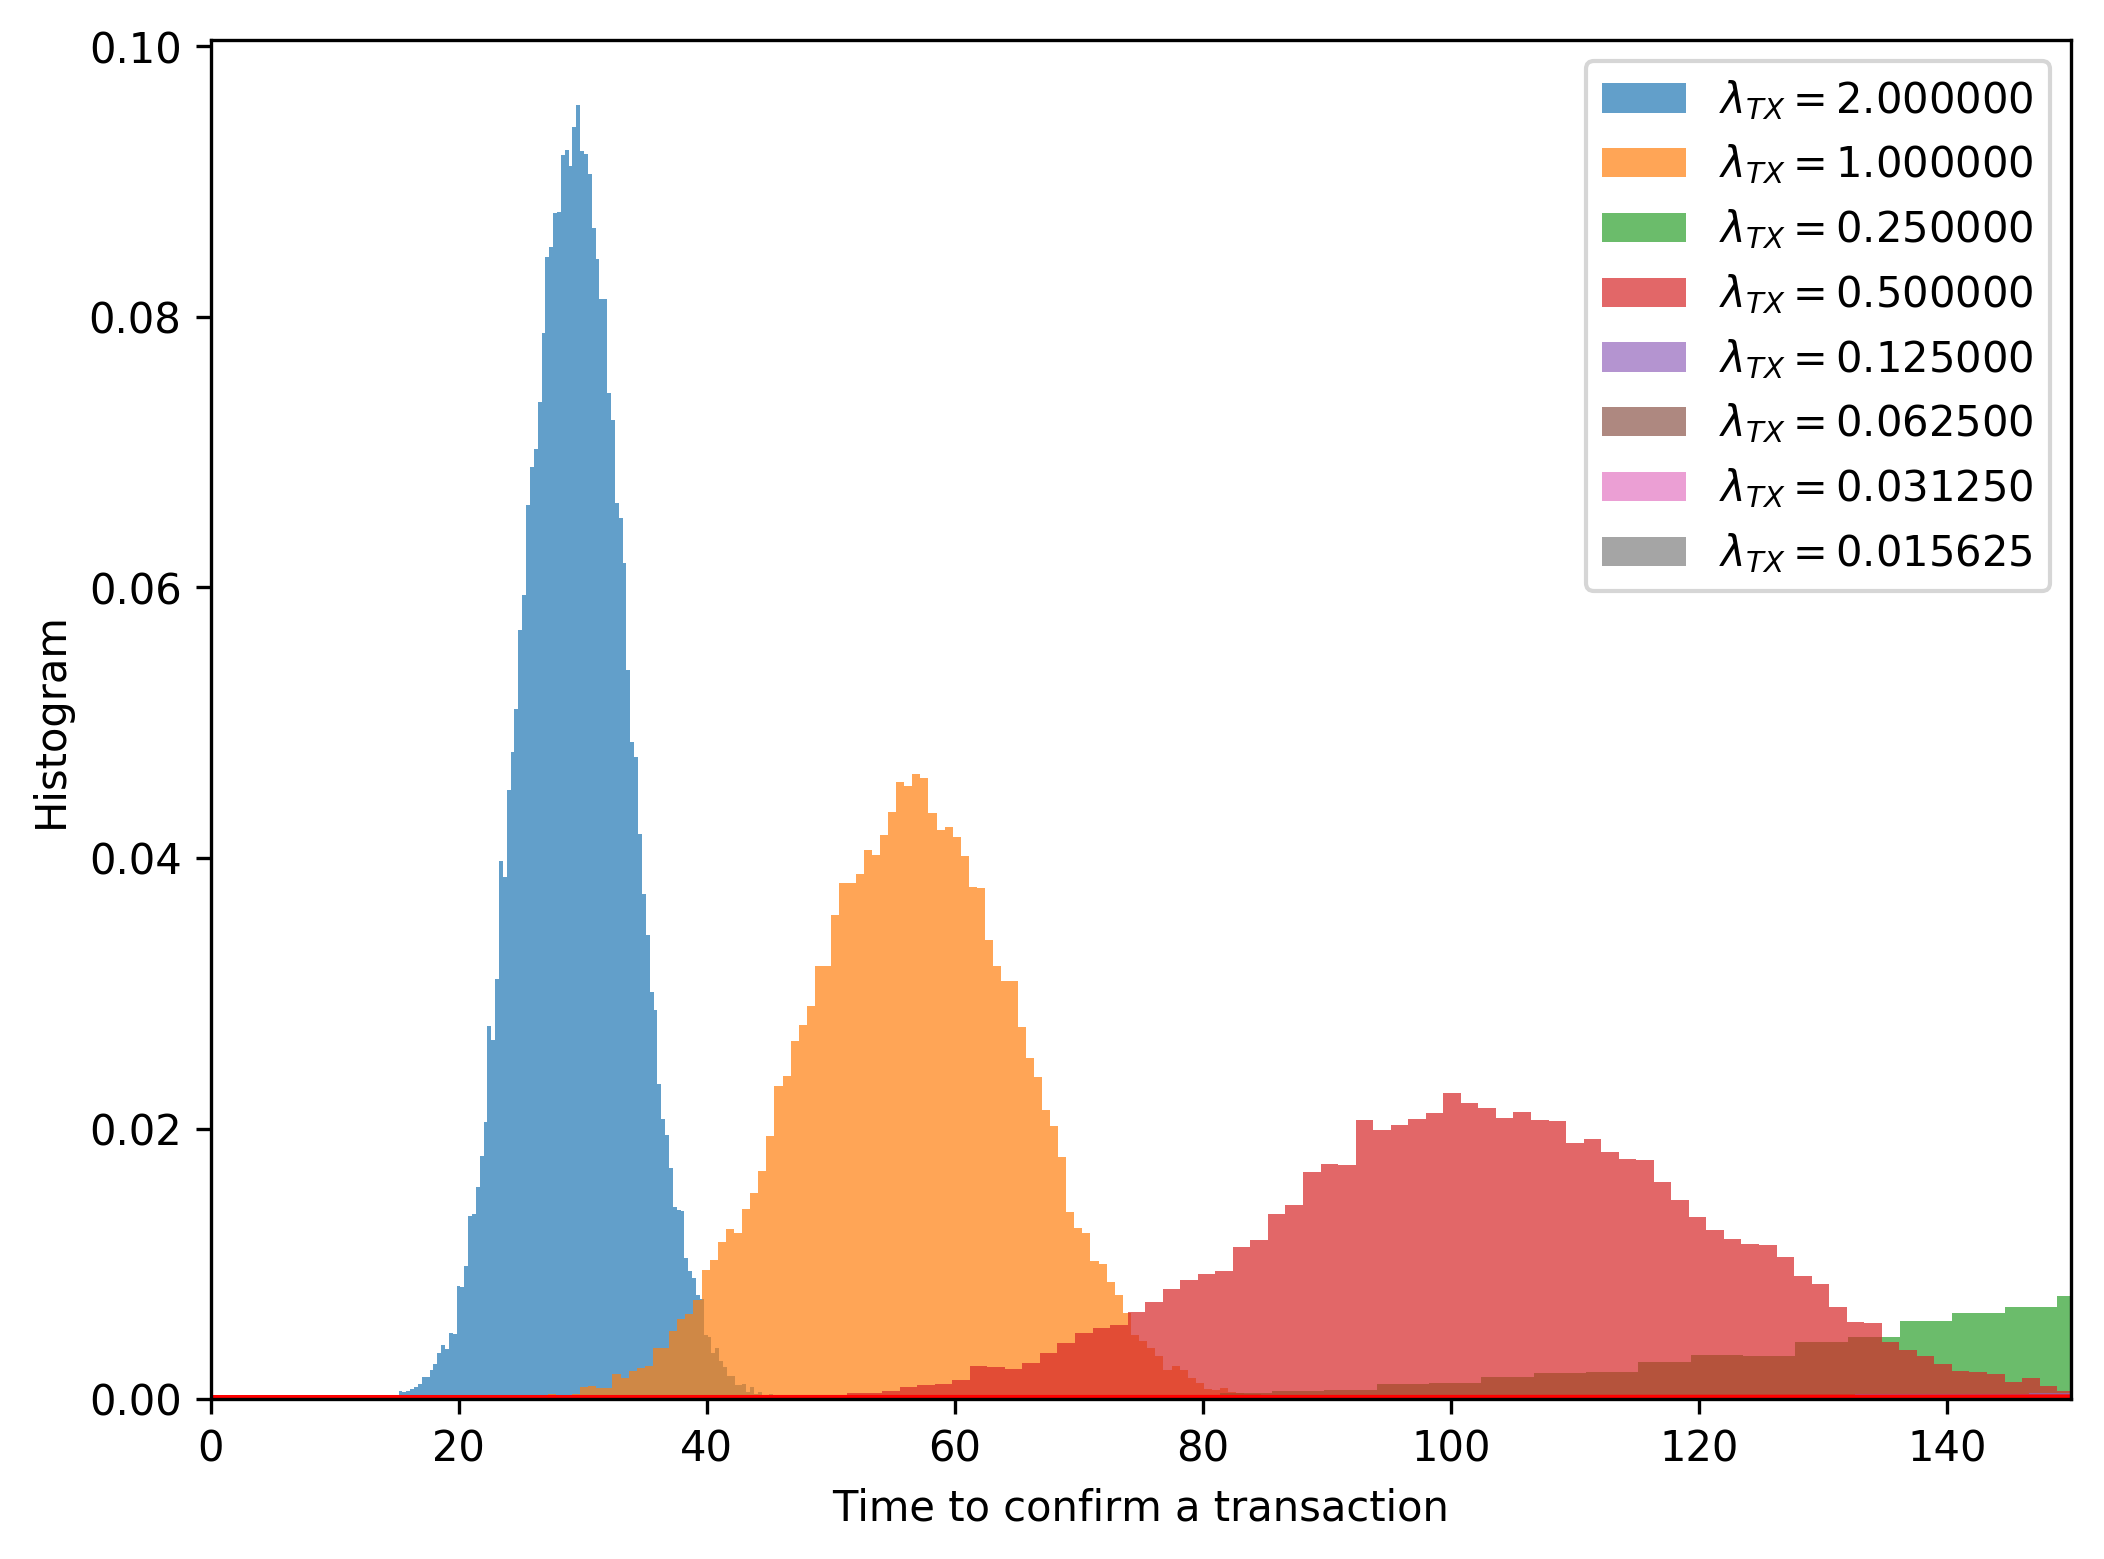
\includegraphics[width=0.5\textwidth]{./images01/sim/tct-many-loads-3.png}}
\subfloat[Zoom in the right part of the above chart \label{fig:hathor-tct-many-right}]{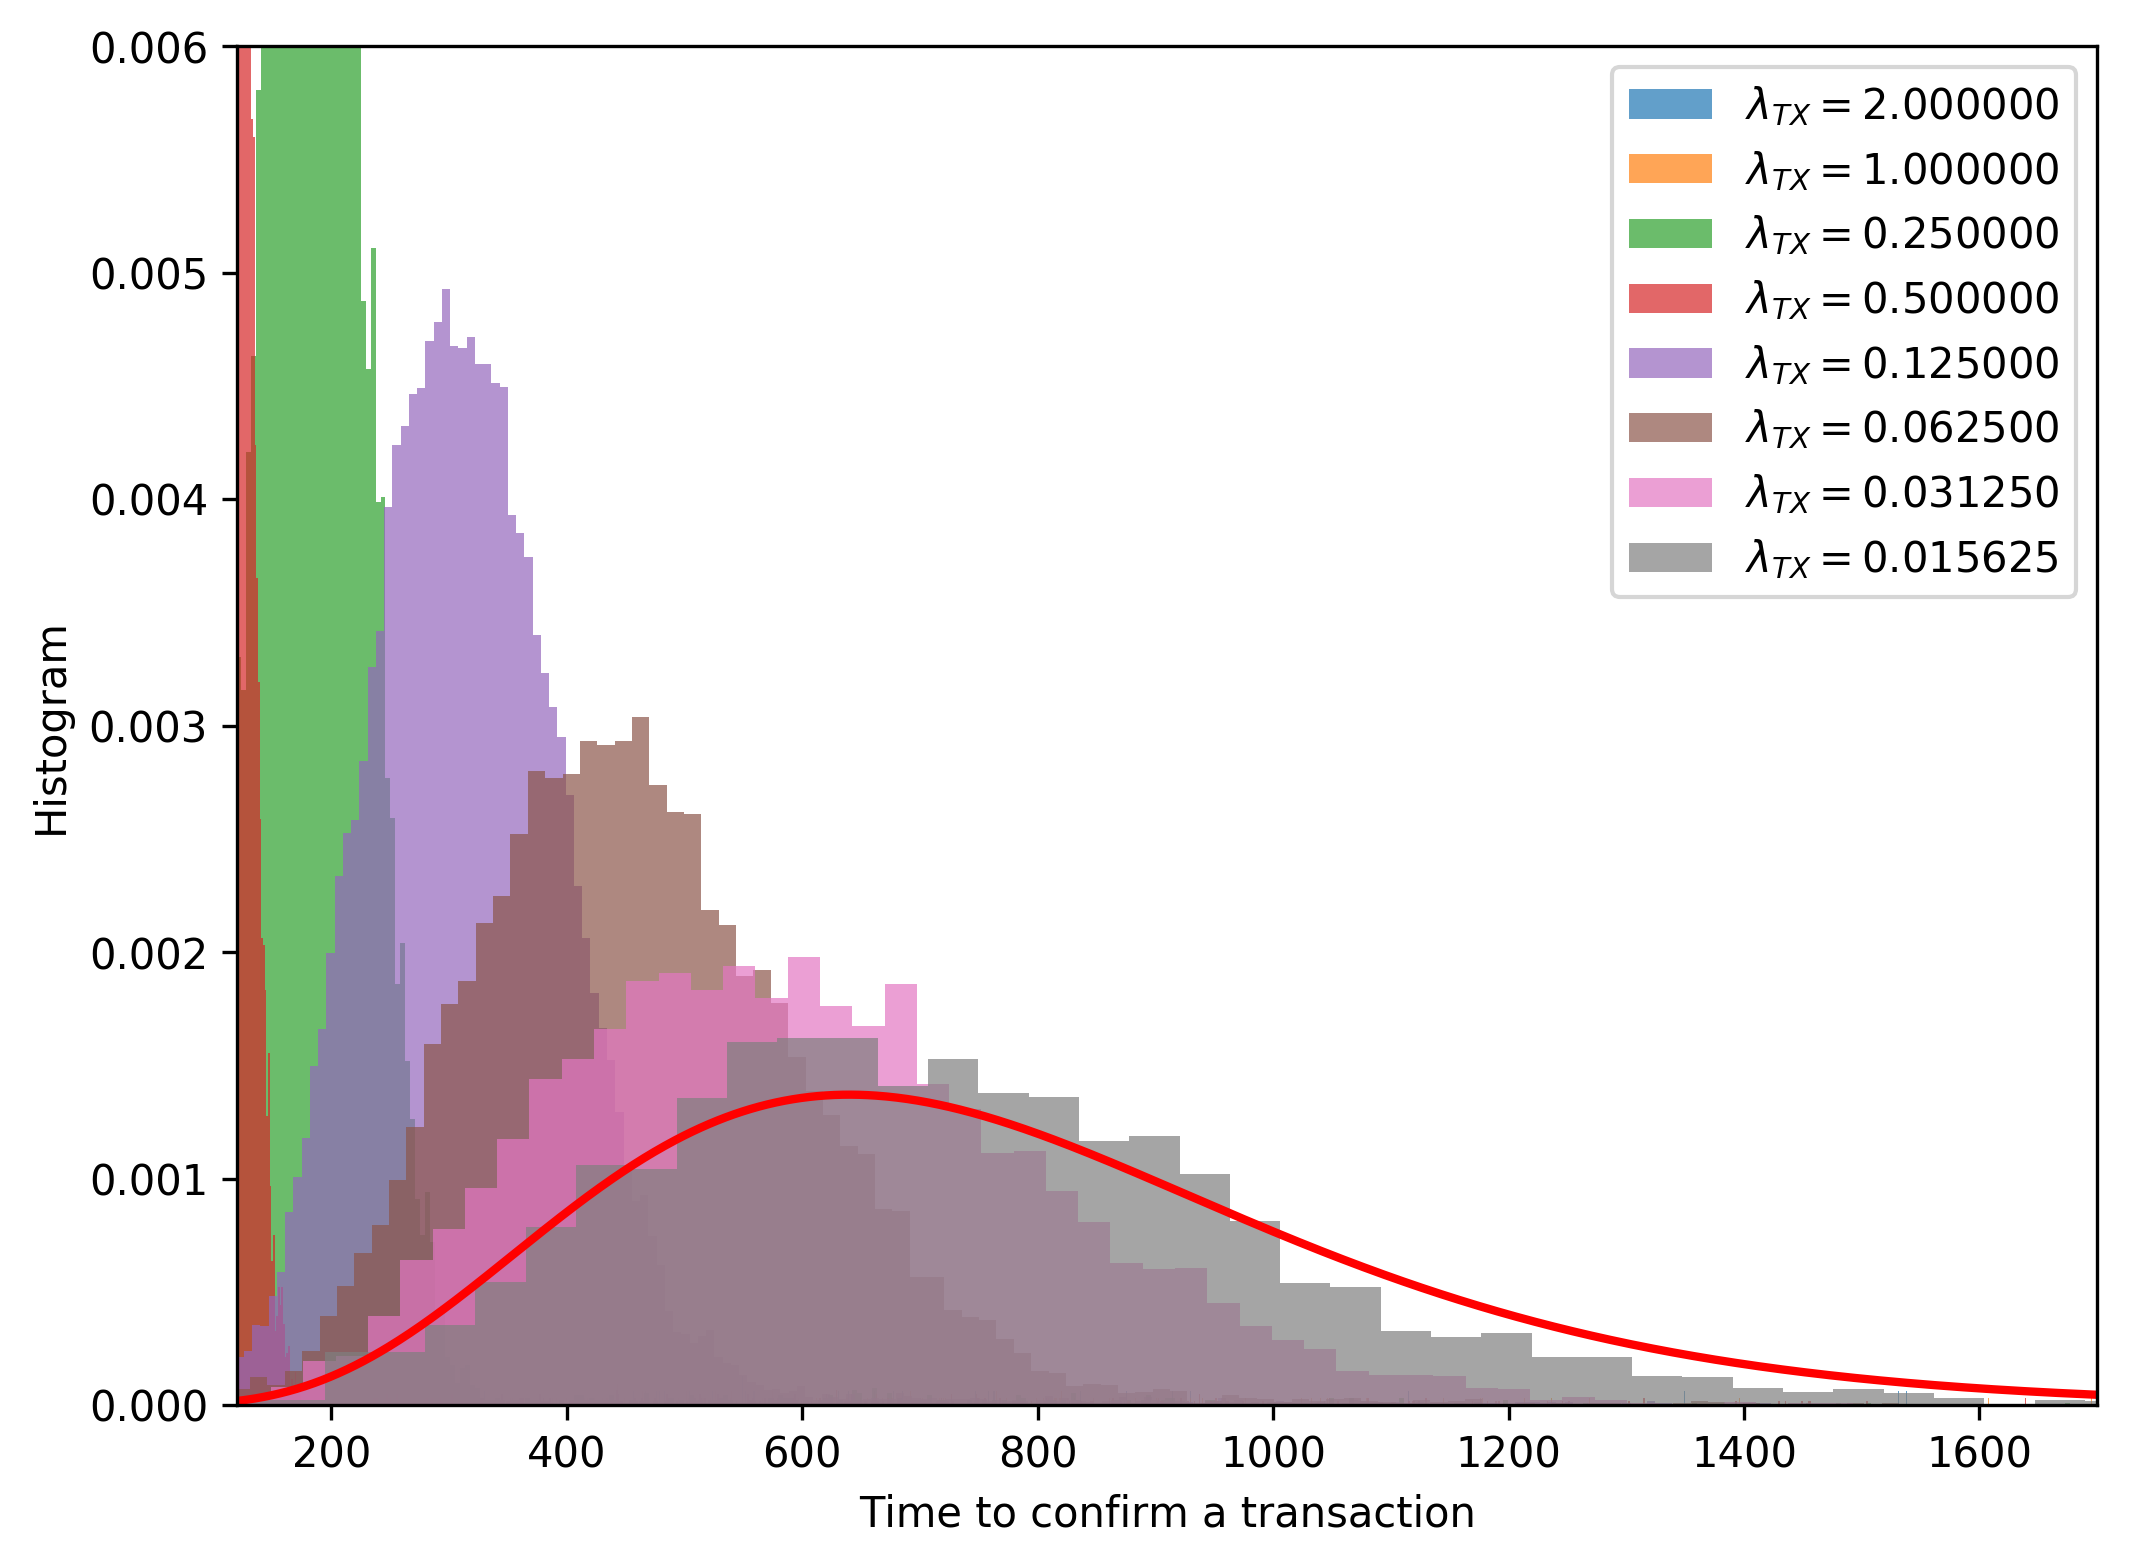
\includegraphics[width=0.5\textwidth]{./images01/sim/tct-many-loads-4.png}}

\caption{Confirmation time in many scenarios, moving from a low load ($\lambda_\text{TX} = 0.015625$) to a high load ($\lambda_\text{TX} = 2$). \label{fig:hathor-tct-many}}
\end{figure}

But, what would happen if, instead of changing the number of transactions per second, we change the relative hash power between miners and transactions? In previous simulations, the miners had a hash rate in the same magnitude as the transactions. In Figure \ref{fig:hathor-tct-100k-10k}, we can see the same simulation as in Figure \ref{fig:hathor-tct-mid-load}, but with the miners' hash rate ten times the transactions'. Besides the difference in the shape of the distribution, we can see that it is moving back towards Bitcoin's confirmation time distribution. It also makes sense because increasing the miners' hash rate increases the required minimum accumulated weighted for confirmed transactions. Therefore, more transactions are necessary to give more accumulated weight. As the number of transactions per second was not changed, most of the work of confirmations were done by blocks (and not by transactions). To confirm this idea, I kept the miners' hash rate ten times the transactions' and increased 16 times the number of transactions per second. As we can see in Figure \ref{fig:hathor-tct-100k-10k-high}, when the number of transactions per second is increased, its role in the accumulated weight also increases and it goes farther from Bitcoin's distribution.

\begin{figure}[!htb]
\centering
\subfloat[Same load as in Figure \ref{fig:hathor-tct-mid-load}]{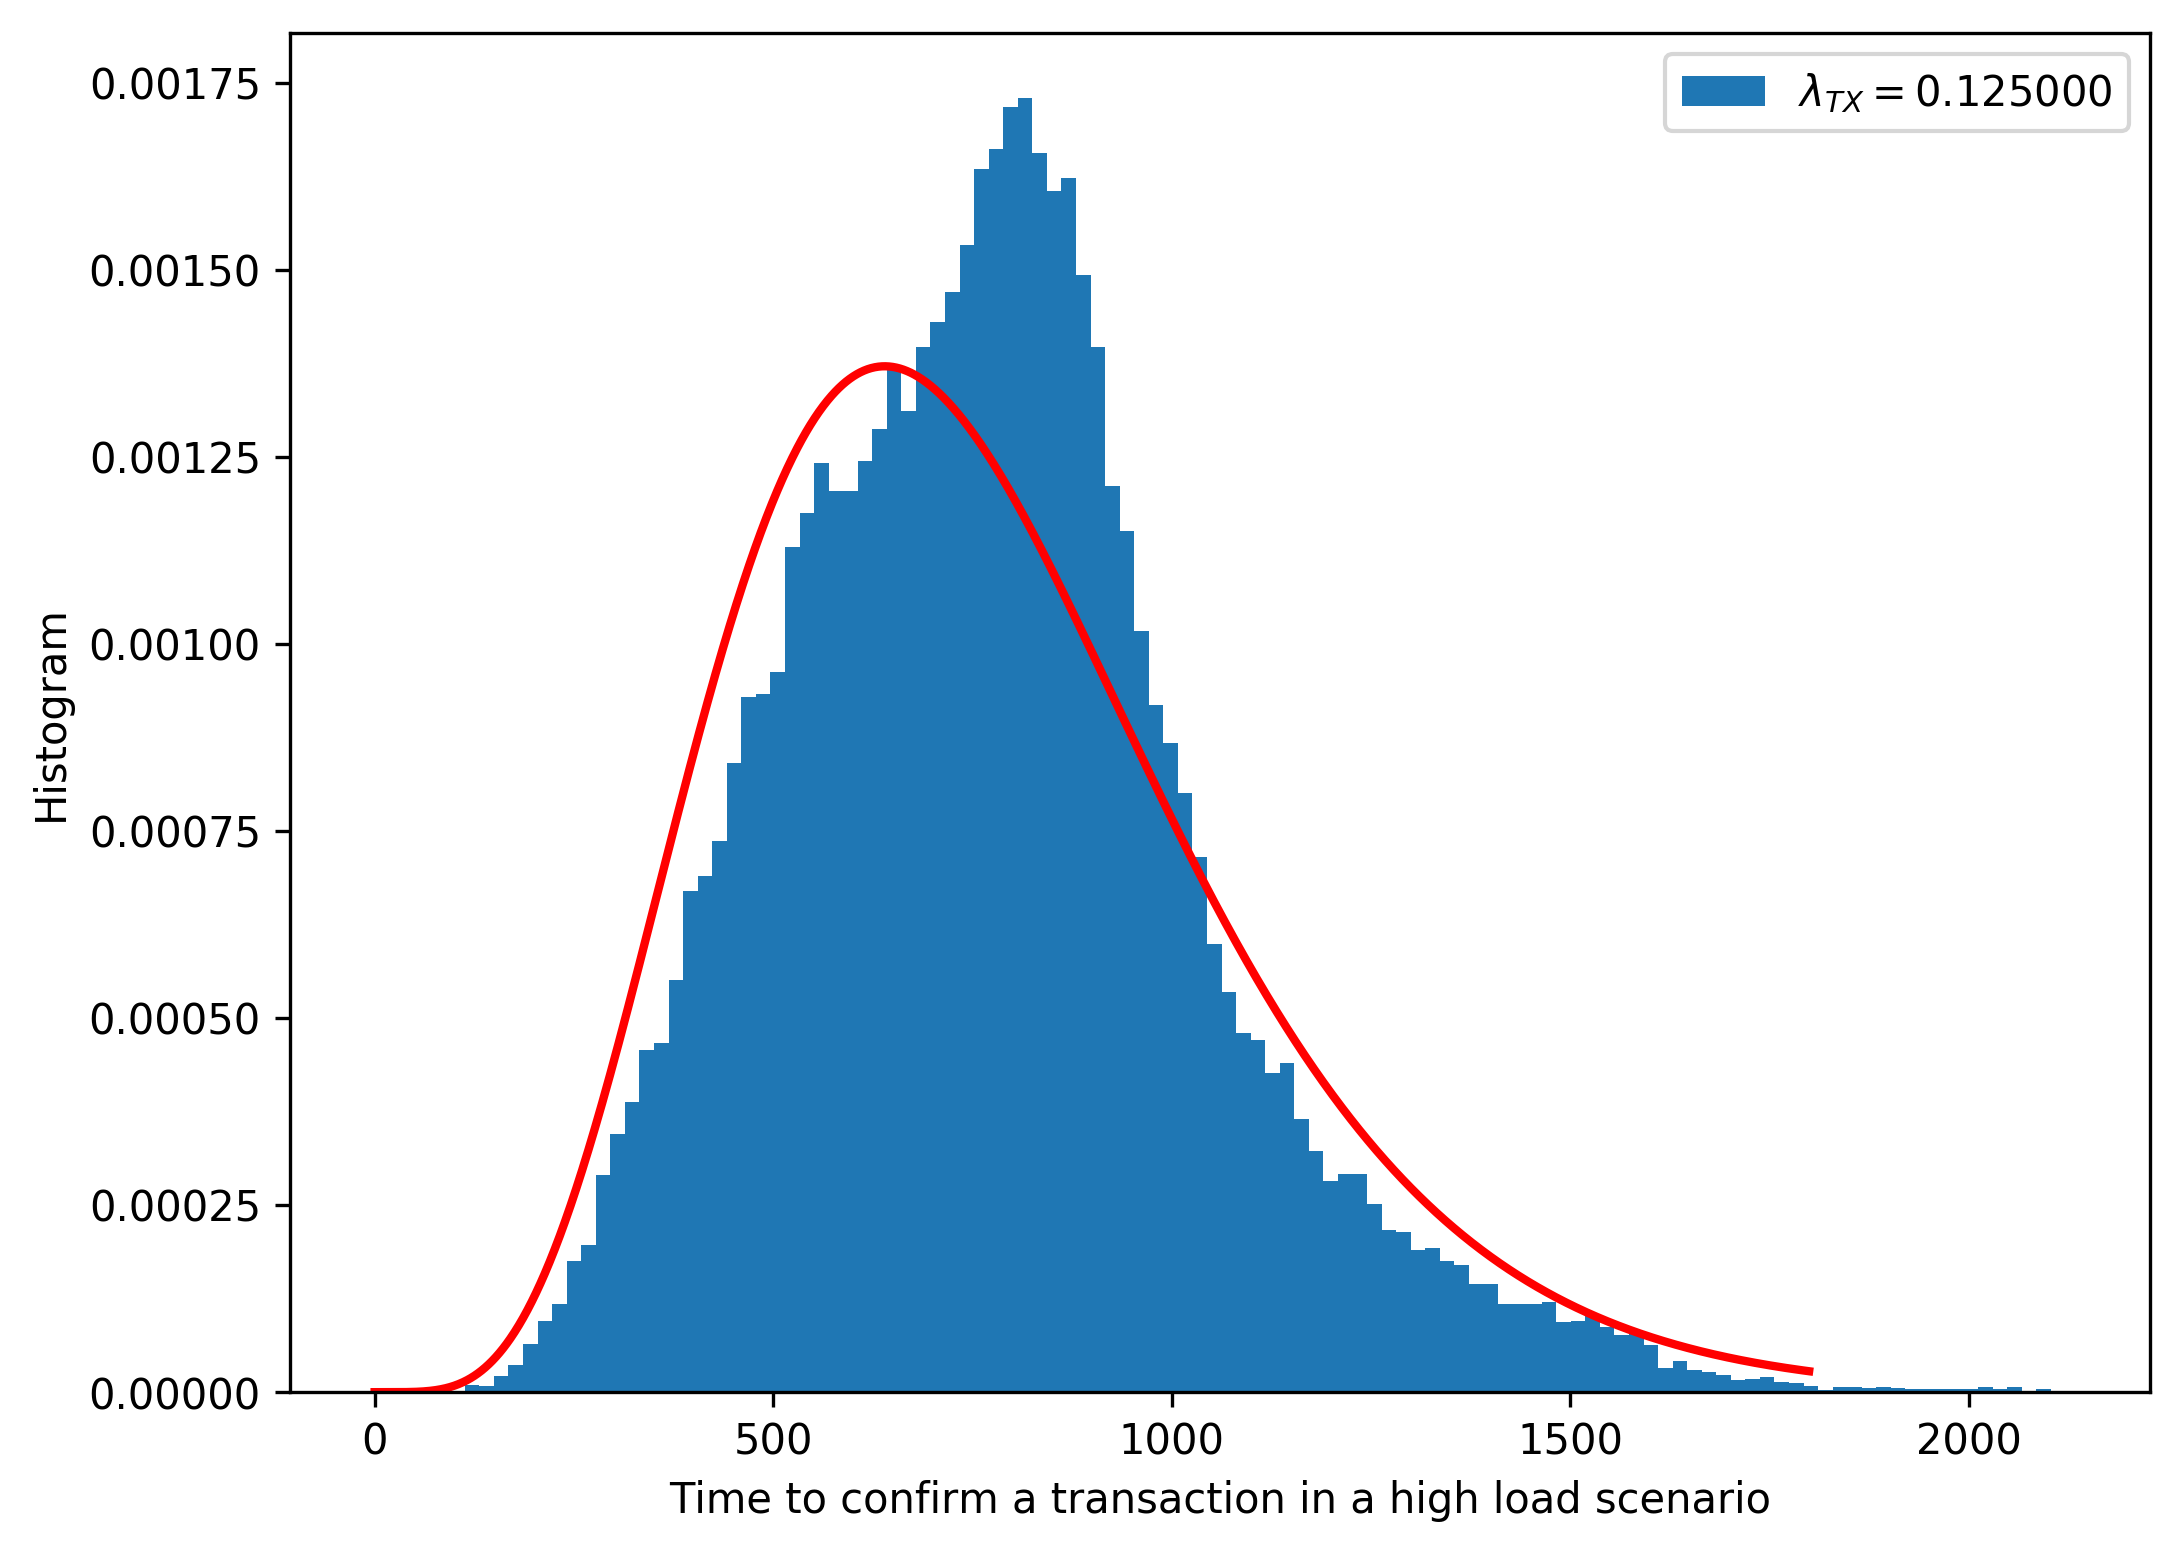
\includegraphics[width=0.5\textwidth]{./images01/sim/tct-100k-10k.png}}
\subfloat[High load, 16 times of (a)\label{fig:hathor-tct-100k-10k-high}]{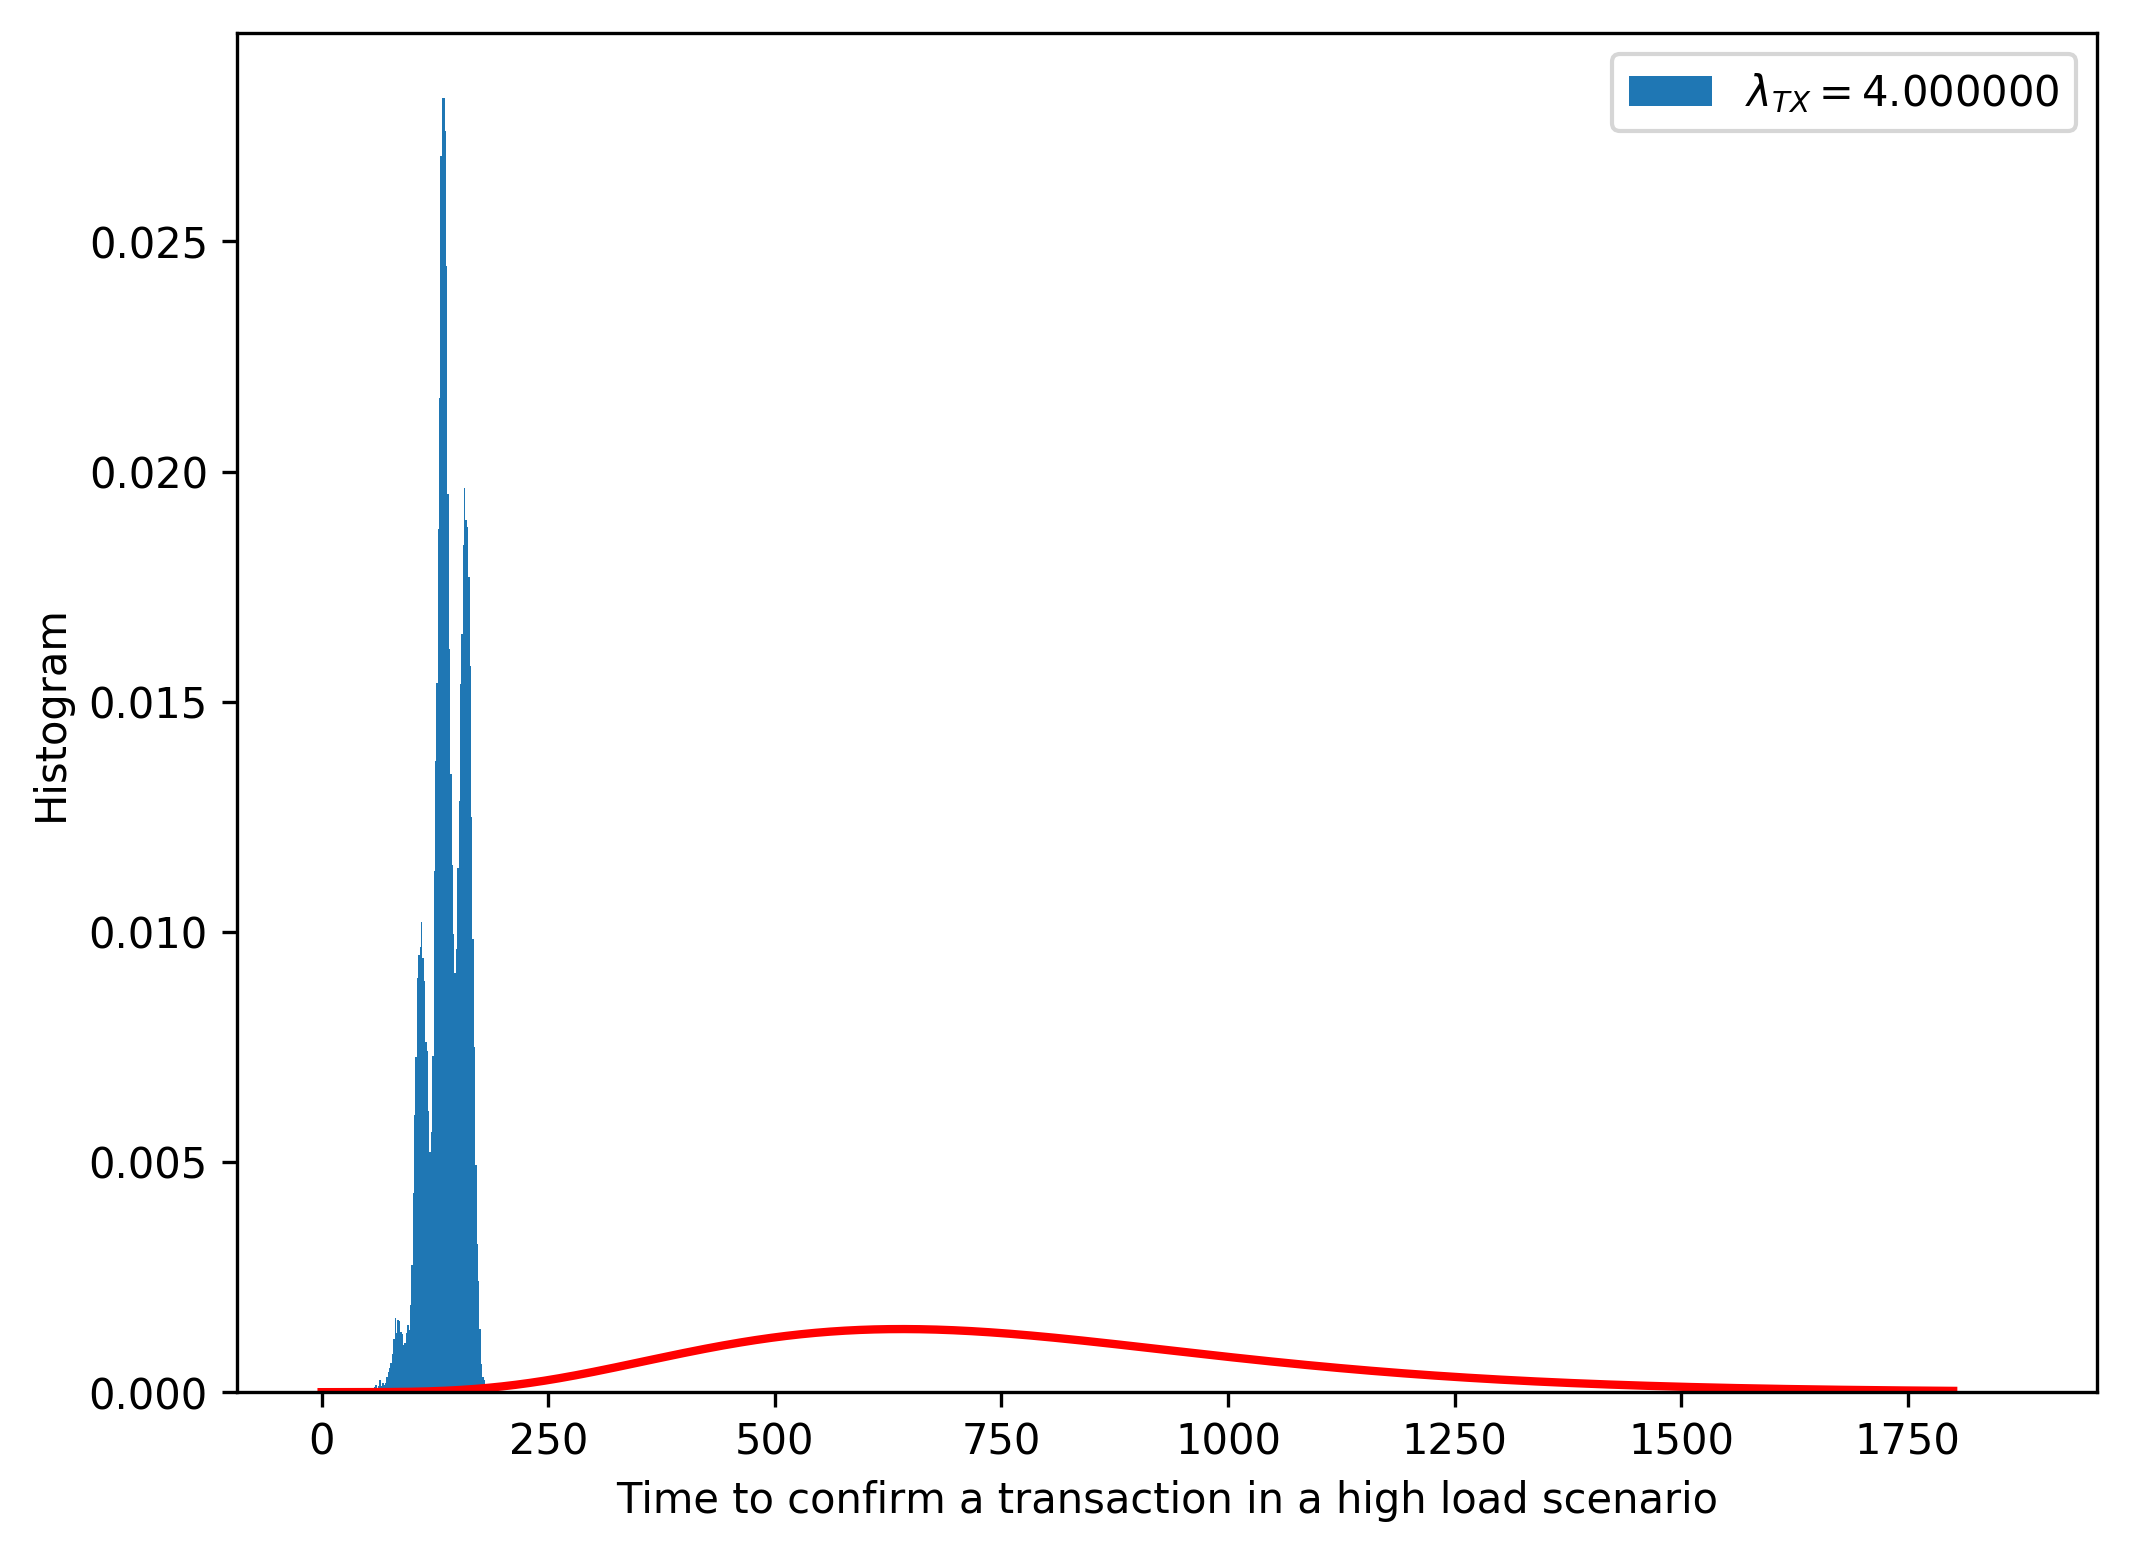
\includegraphics[width=0.5\textwidth]{./images01/sim/tct-100k-10k-high-load.png}}

\caption{Confirmation time with miners' hash rate ten times the transactions'. \label{fig:hathor-tct-100k-10k}}
\end{figure}

Finally, even with both blocks and transactions, Hathor's blocks are similar to Bitcoin's blocks, and they share the same math. To confirm that, see Figure \ref{fig:hathor-tbb}, where the red curve is Bitcoin's distribution of time between blocks and the blue histogram is Hathor's time between blocks. I also made several tests adding and removing miners to check the difficulty adjustment and it worked properly.

\begin{figure}[!htb]
\centering
\subfloat[1 miner]{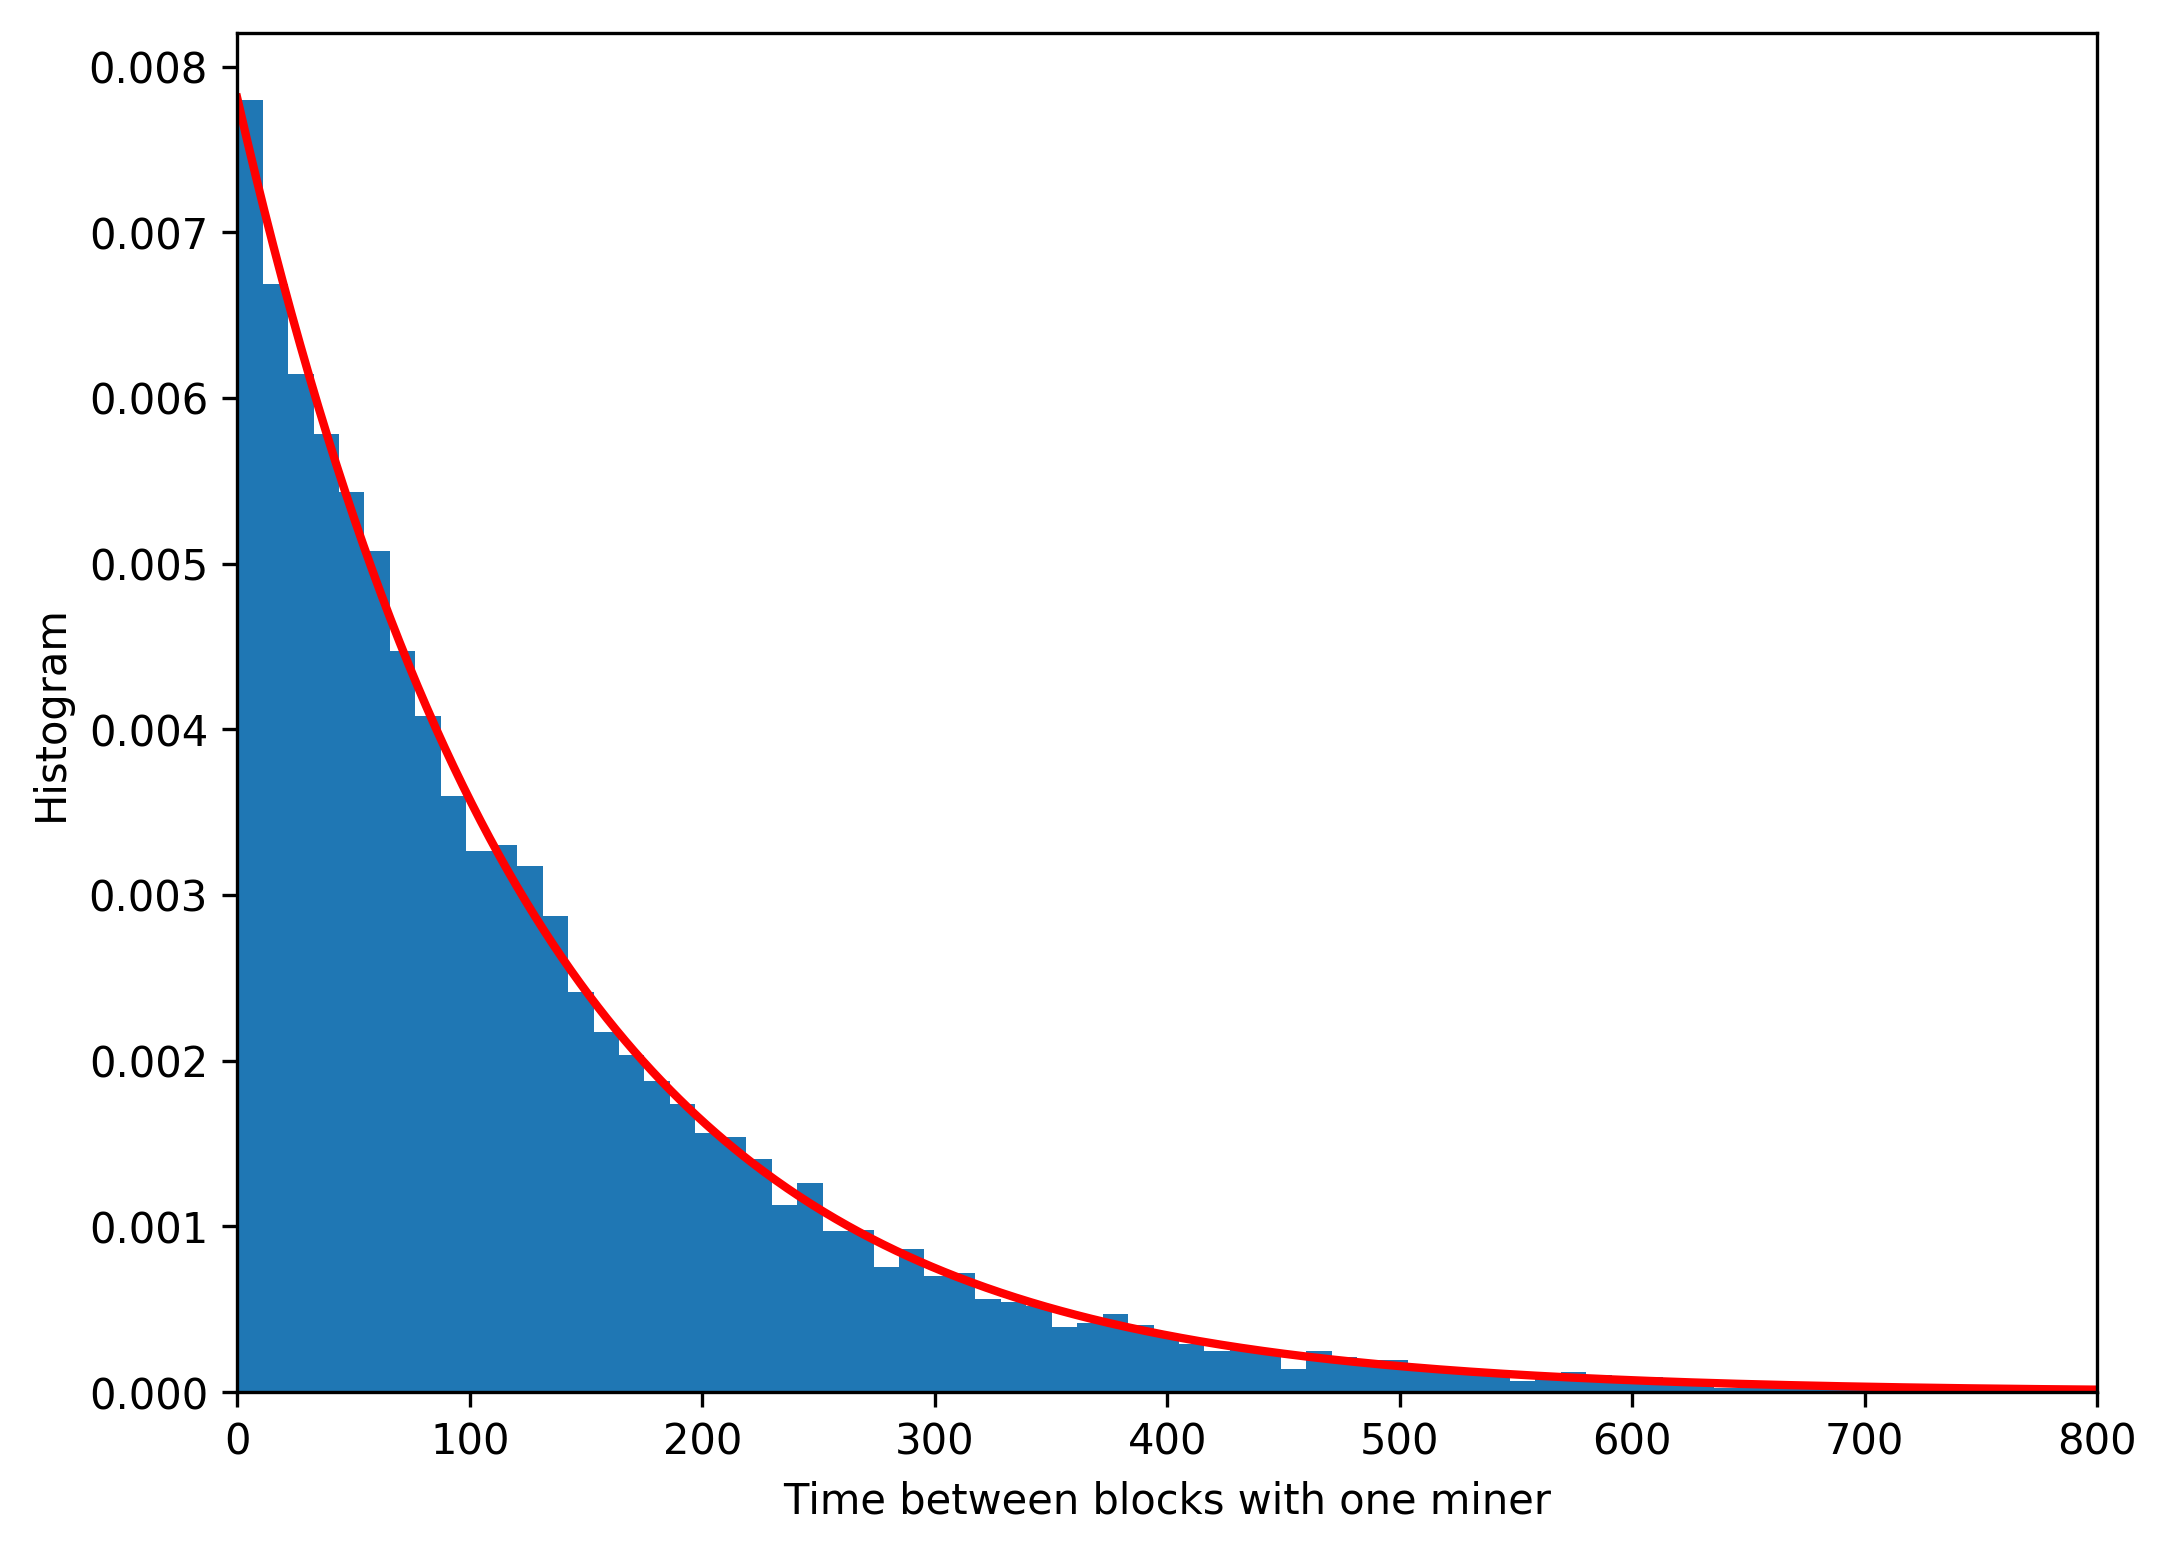
\includegraphics[width=0.5\textwidth]{./images01/sim/tbb-1.png}}
\subfloat[2 miners after difficulty adjustment]{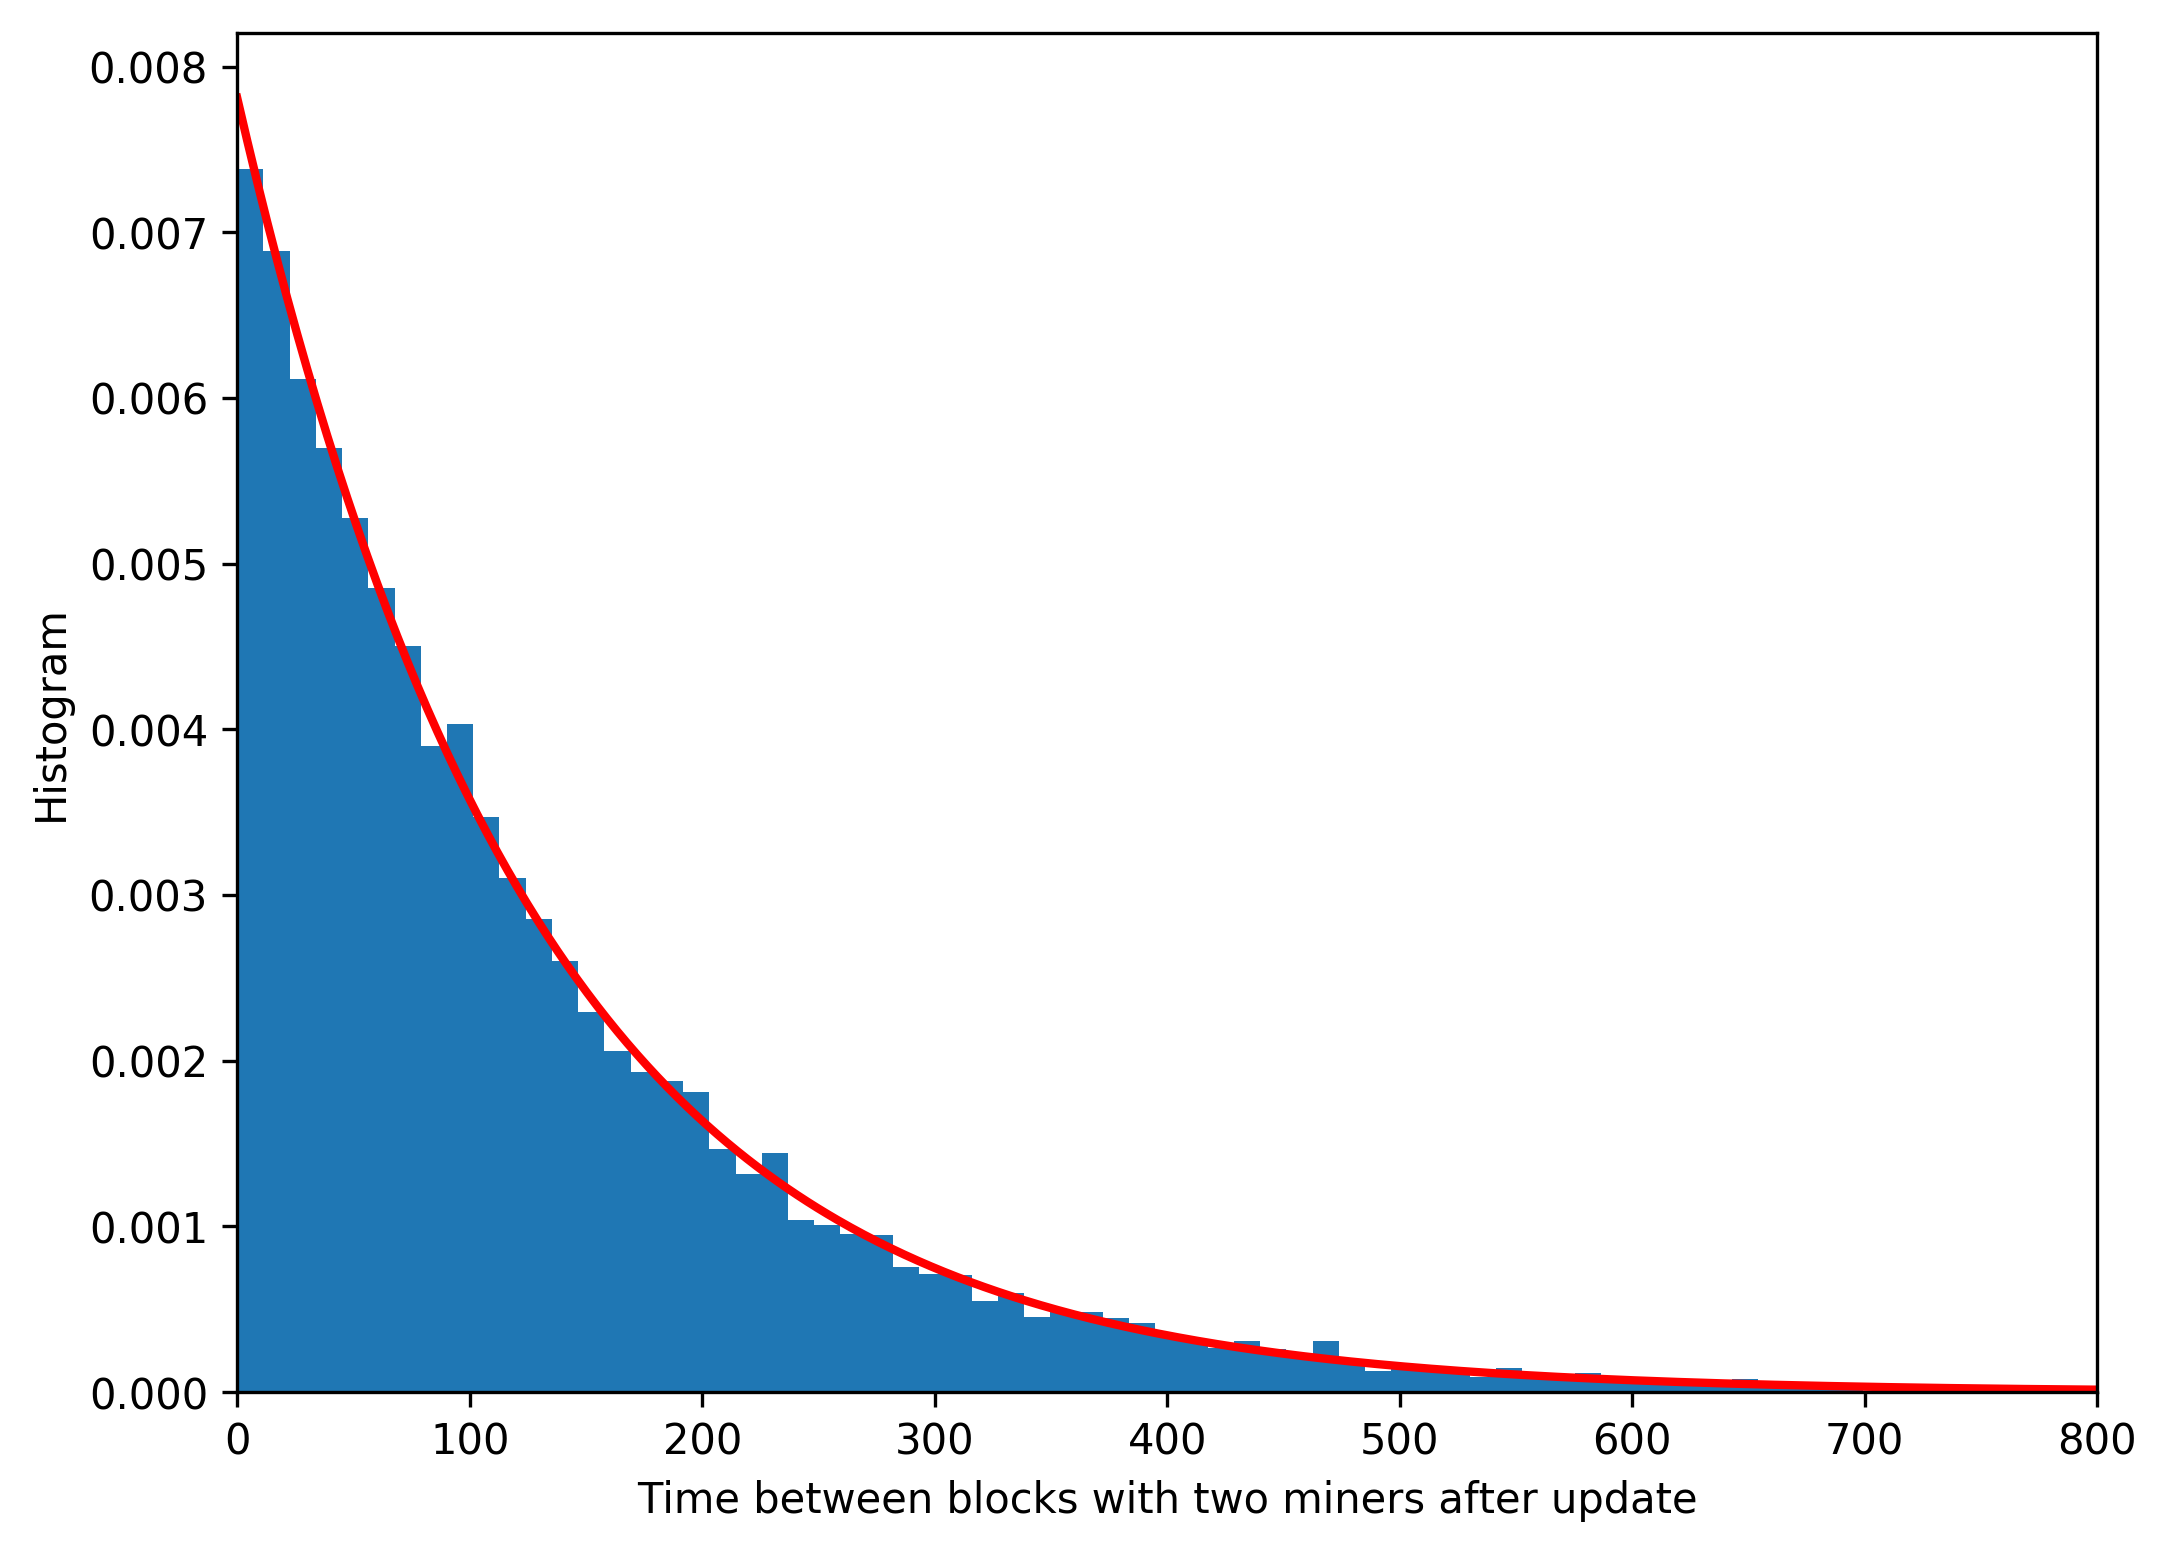
\includegraphics[width=0.5\textwidth]{./images01/sim/tbb-2-after.png}}

\caption{Histogram of time between blocks. The red curve the Bitcoin's theoretical distribution of time between blocks. As we can notice, the fit is very good. \label{fig:hathor-tbb}}
\end{figure}

\clearpage

\begin{figure}[!htb]
\centering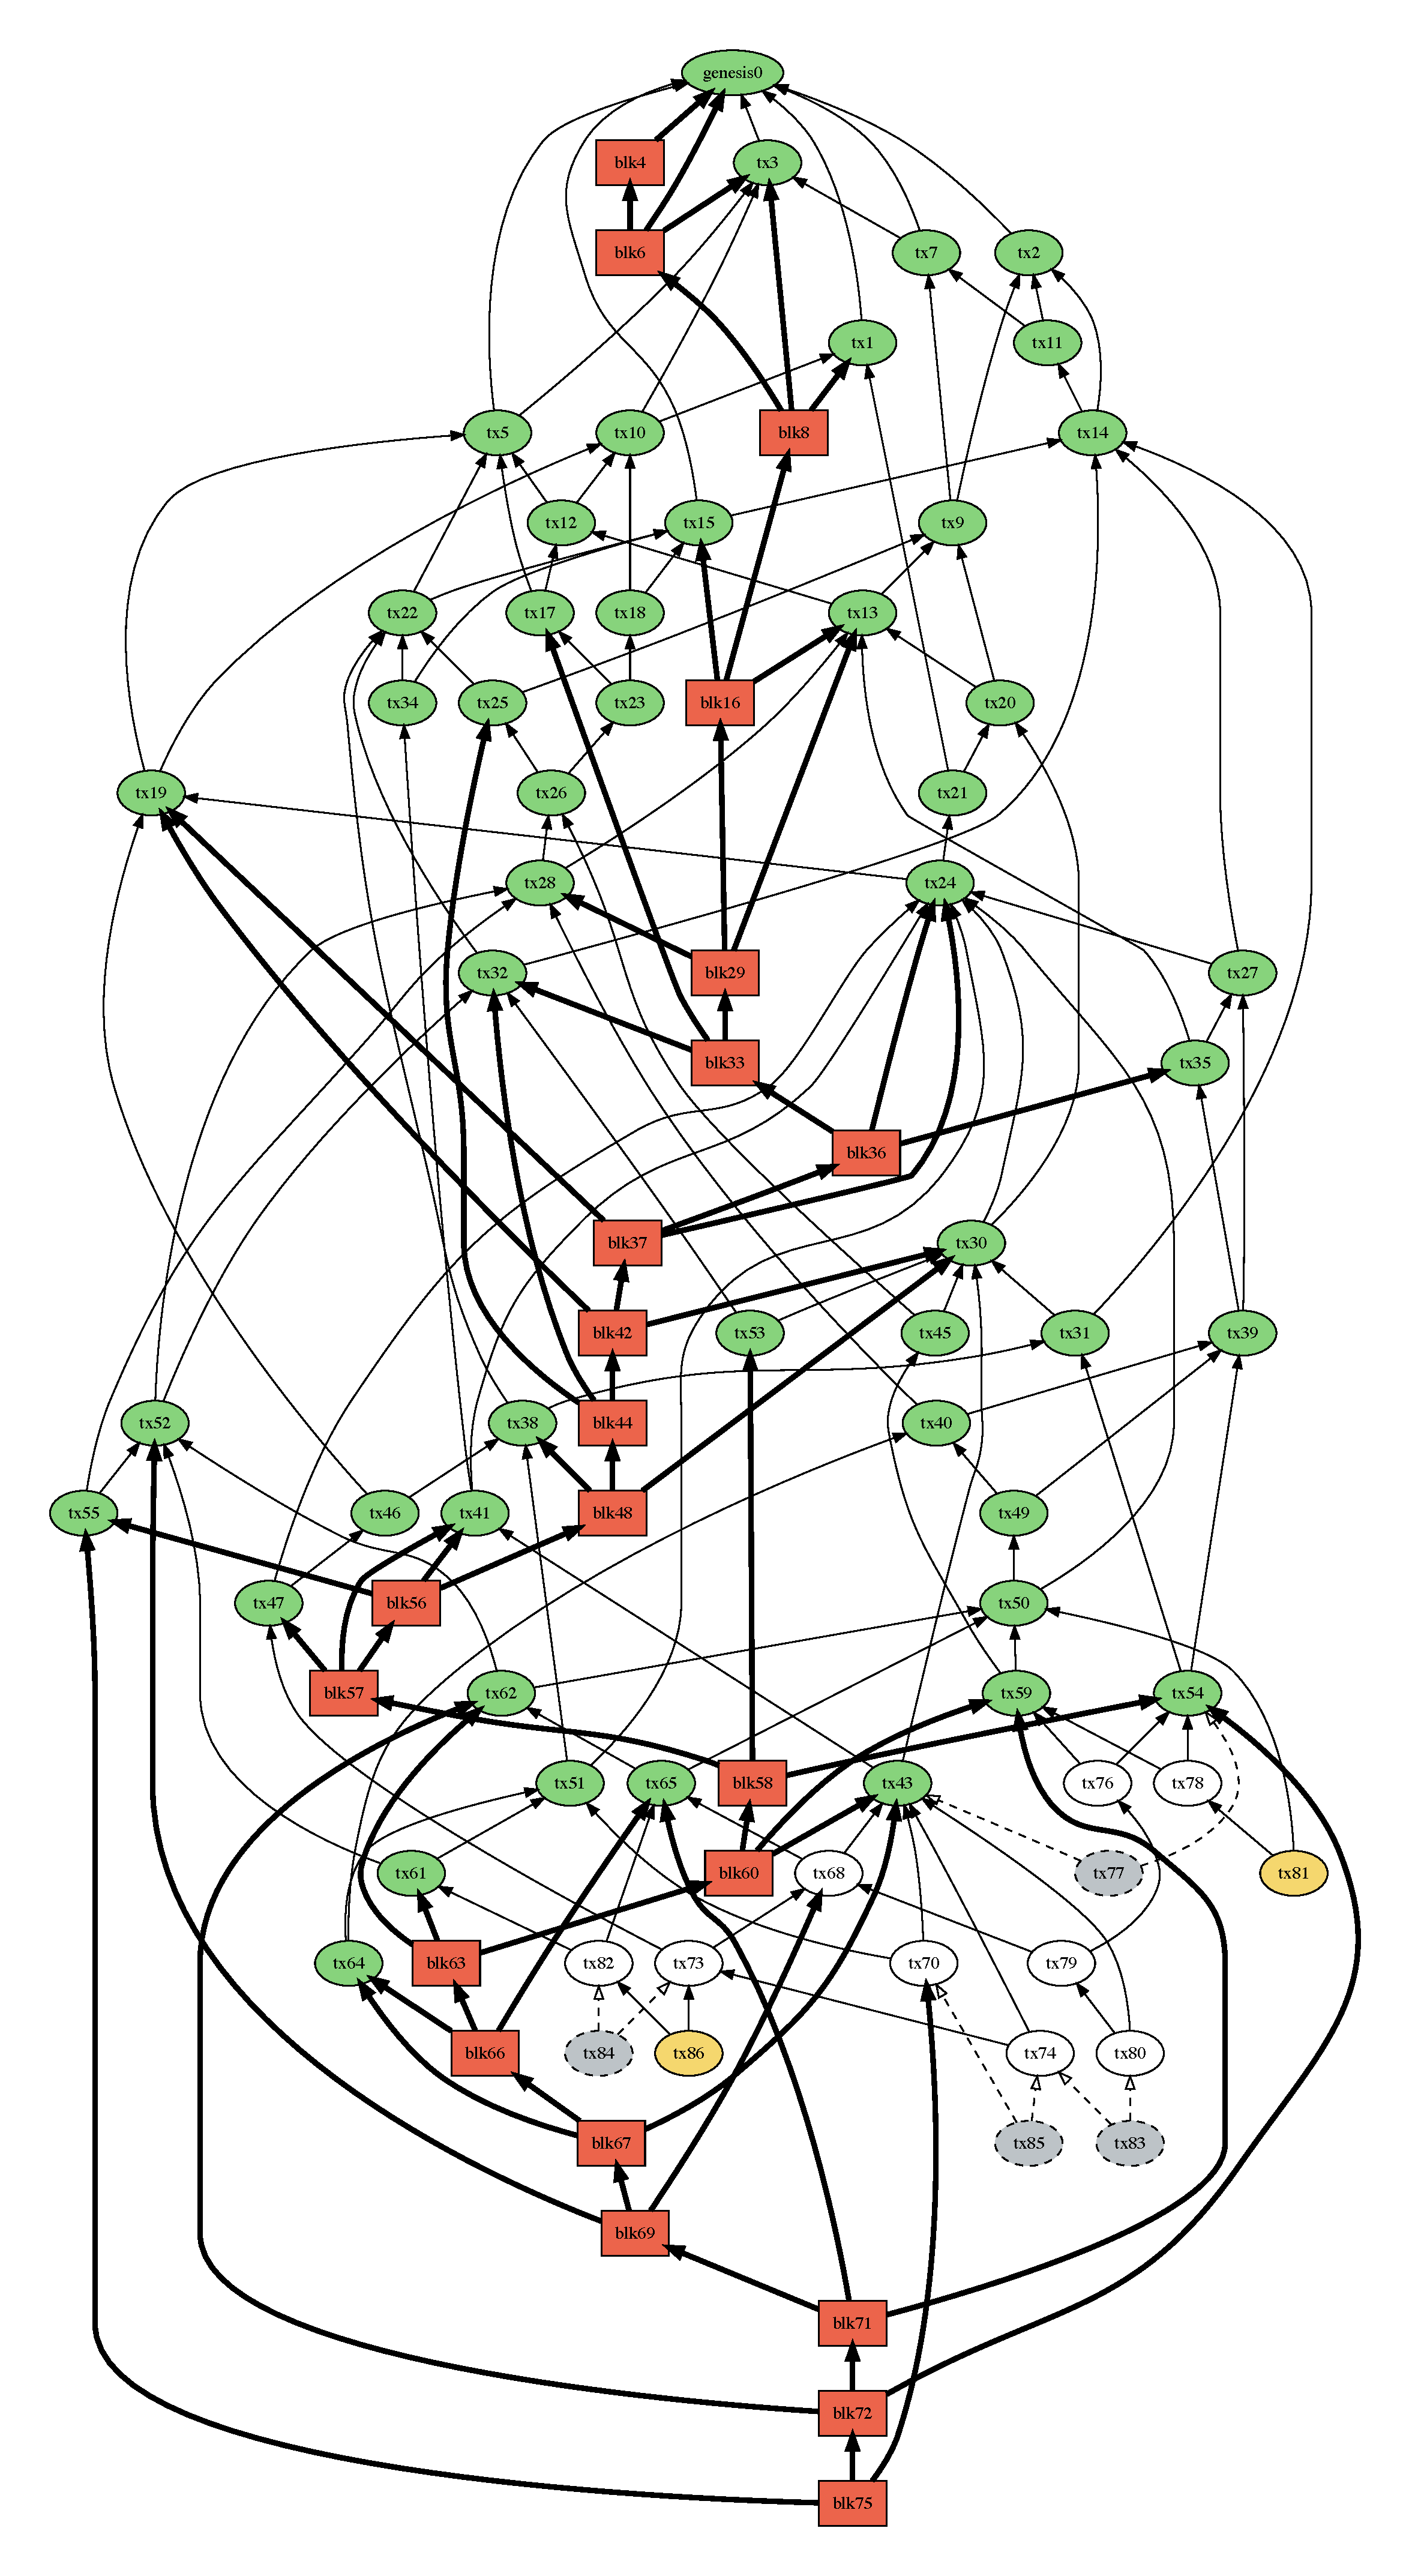
\includegraphics[width=\textwidth]{./images01/sim/hathor-2.pdf}
\caption{Visualization of a Hathor's graph with transactions and blocks. Red boxes are blocks; green circles are confirmed transactions; white circles are in-progress transactions; yellow circles are unconfirmed transactions (tips); and grey circles are transactions solving the proof-of-work which have not been propagated yet. The arrows show the confirmation chain. Block's arrows are in bold. \label{fig:hathor-dag-big}}
\end{figure}

\clearpage


\section{Visualizing the network}

Visualizing the network is not simple because the number of transactions and blocks is high, thus, arranging them and their edges is a non-trivial task. Therefore, most of the visualization are just part of the DAG which shows a window of time.

To a better visualization of a Hathor's network, I run a simulation classifying the transactions in either confirmed, in-progress, or unconfirmed (tips). I also showed the transactions solving the proof-of-work which had not been propagated yet. See Figure \ref{fig:hathor-dag-big} and notice the chain of blocks inside the DAG. Confirmed transactions are in green circles, while in-progress transactions are in white circles and tips are in yellow circles. The blocks are in red boxes form a chain inside the DAG. Finally, the new transactions which are solving the proof-of-work and had not been propagated are in grey dashed circles.

As new transactions have to chose two previous transactions to confirm, and just after they start to work in the proof-of-work, two new transactions eventually may chose the same tip because they do not know each other yet. So, if new transactions are coming in a low pace, the width of the swarm is small because the number of new transactions simultaneously solving the proof-of-work is also small. But, when new transactions are coming in a high volume, the width of the swarm increases because new transactions are choosing the same tip over and over.

In summary, the width of the swarm depends on the number of transactions per second. The greater the number of new transactions per second, the larger the width of the swarm.

To visualize the change in the width of the swarm, I run a simulation with a constant number of transactions per second, which was increased only in a specific window of time. The result can be seen in Figure \ref{fig:hathor-load-changing}, where the number of transactions per second suddenly increases, and the width increases until it reaches a stable value. Then, the number of transactions per second decreases, and the width returns to the previous value.

\begin{figure}[!htb]
\centering
\includegraphics[width=\textwidth]{./images01/new/many-loadings.pdf}

\caption{DAG visualization when the loading is changed over time. \label{fig:hathor-load-changing}}
\end{figure}






\section{Number of tips}

The number of tips at a given time also depends on the number of new transactions per second. The relationship between them was empirically measured in several simulations with different $\lambda_\text{TX}$.

Analyzing Figure \ref{fig:hathor-tips}, it is easy to notice that both the average and the standard deviation of the number of tips increase when $\lambda_\text{TX}$ increases. According to \citet{tangle2016}, the average has the following equation:

$$\frac{\lambda_\text{TX}}{\log(2)} \frac{2^{w_\text{TX}}}{H}$$

In our simulation, $H = 100,000$ and $w_\text{TX} = 17$, so, the average number of tips should be equal to $1.89 \cdot \lambda_\text{TX}$. This model works best for low values of $\lambda_\text{TX}$ and diverges a little for higher values. For instance, if $\lambda_\text{TX} = 32$ tx/s, this equation predicts $60.48$ tips on average yet we can check in the empirical result that the average is around $55$ tips.

When $\lambda_\text{TX} \rightarrow 0$, the number of tips goes towards one. The explanation is that there will be only one new transaction solving the proof-of-work per turn. So, new transactions will always confirm two tips, reducing the number of tips by one---each transaction confirms two tips and create one new one, hence the balance is -1. As it is impossible to have less to have less than one tip, it converges to one.

When there is only one tip, new transactions must chose this only tip and another in-progress transaction. It should only happen in very low load scenarios, like during the launch of the network itself.

\begin{figure}[!htb]
\centering
\subfloat[All load scenarios]{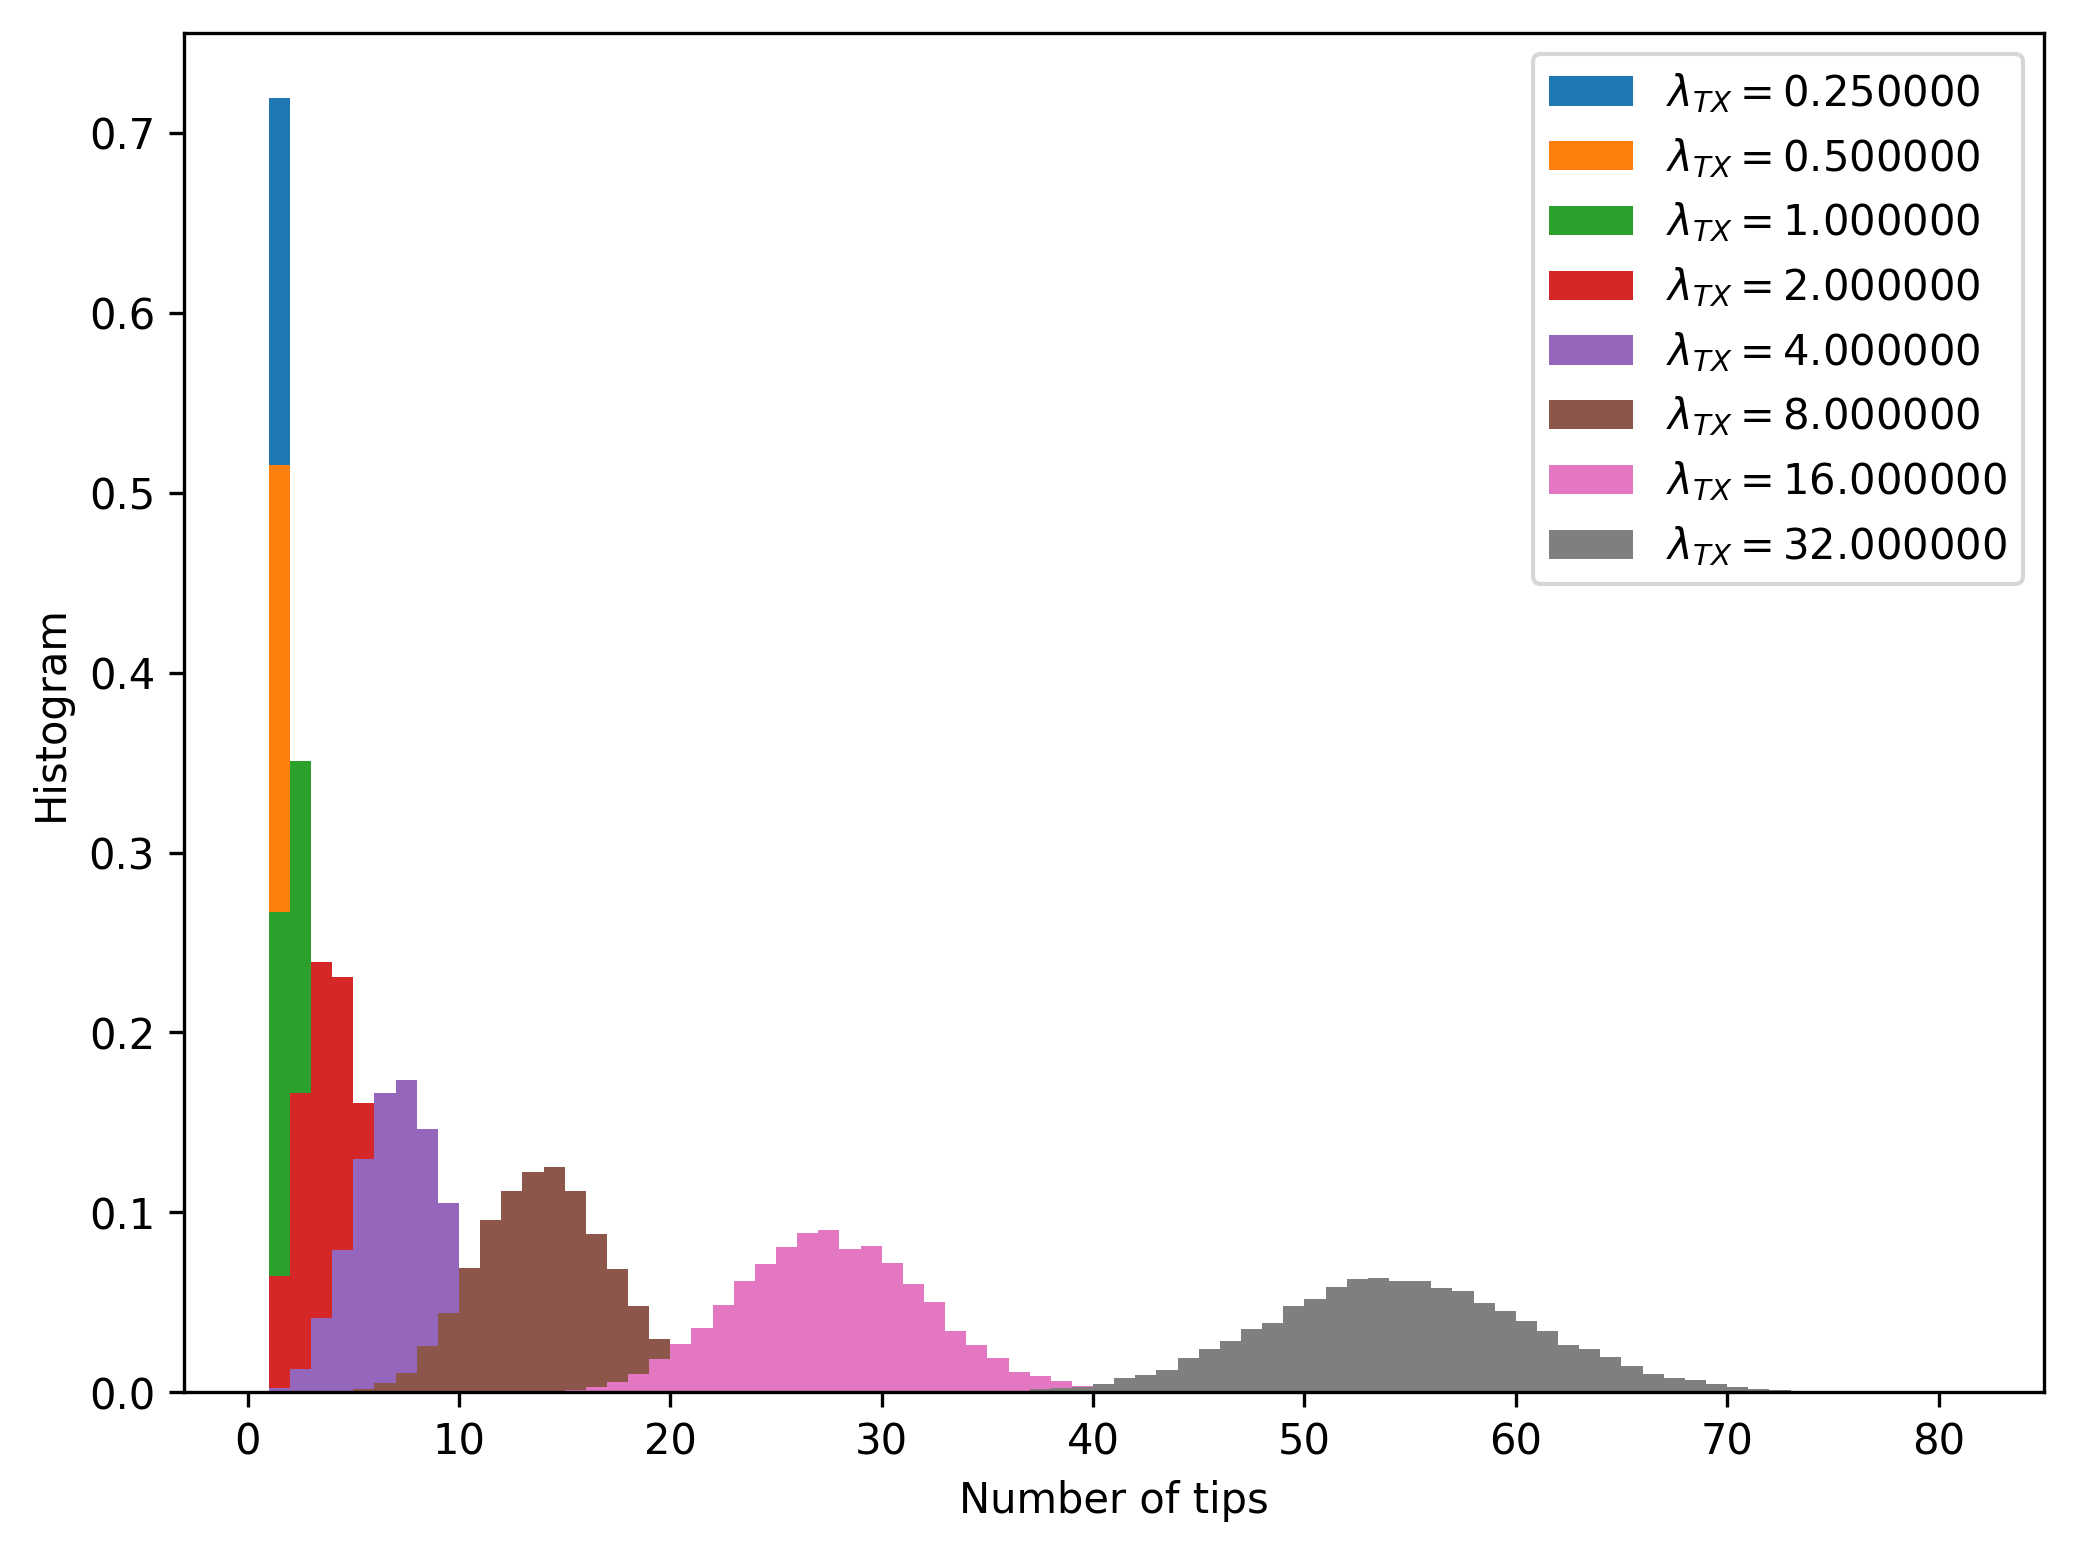
\includegraphics[width=\textwidth]{./images01/new2/tips_aggregate.png}}

\subfloat[Zoom in the left side of (a)]{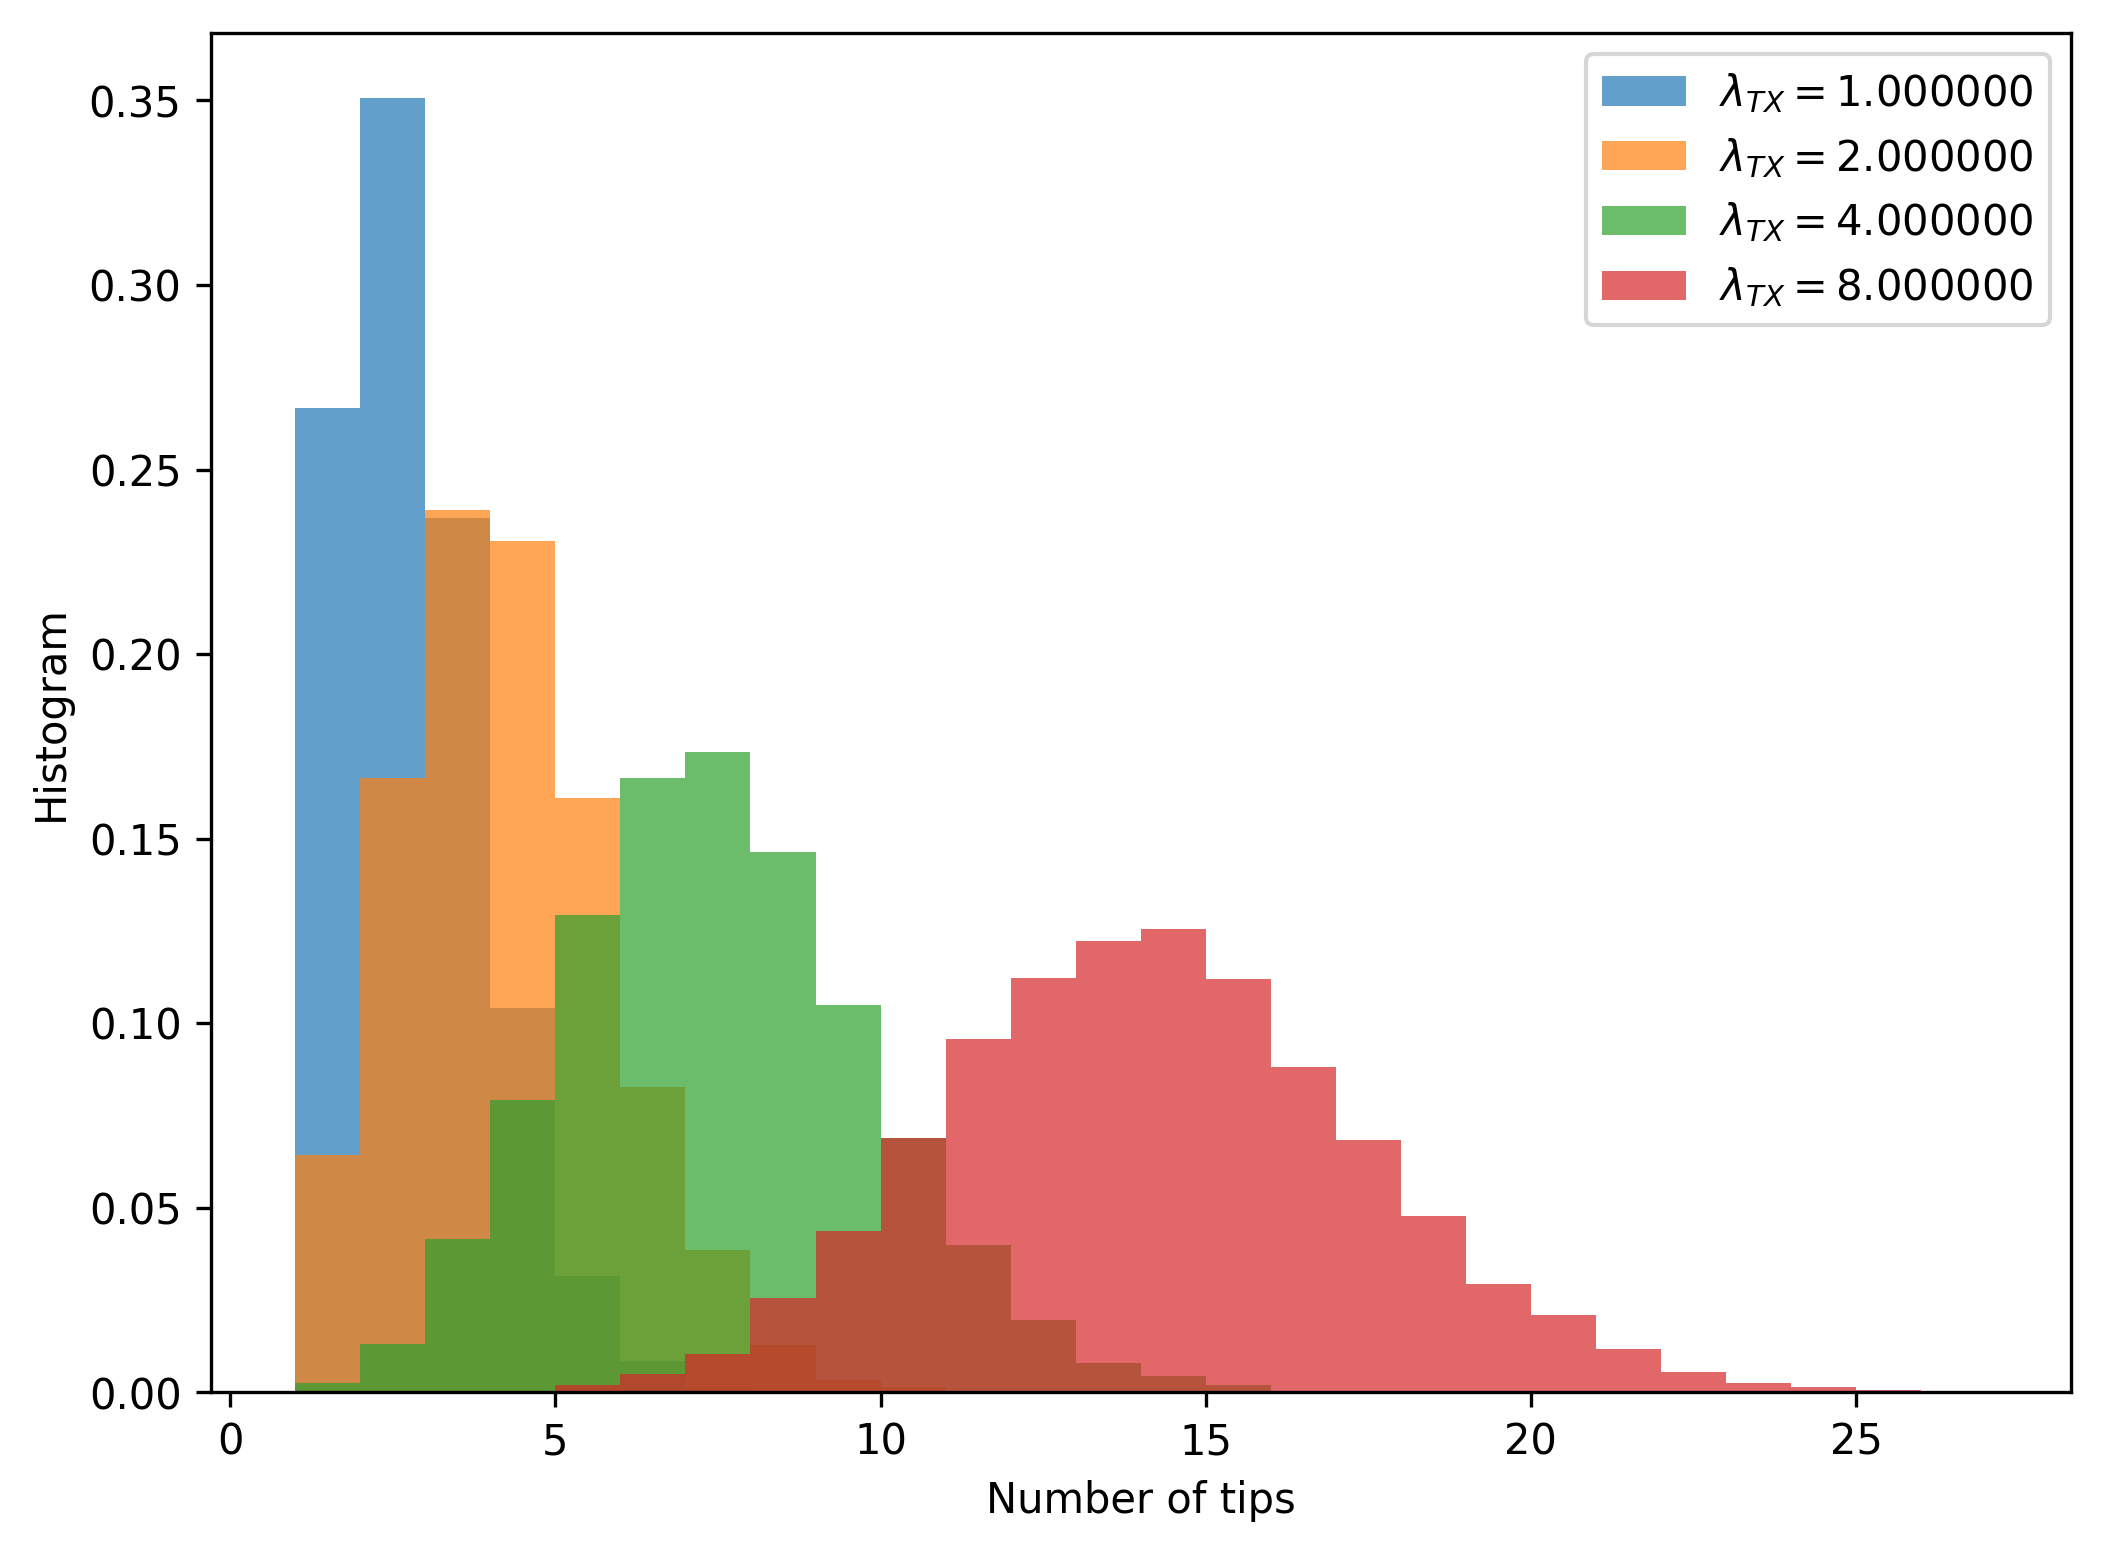
\includegraphics[width=\textwidth]{./images01/new2/tips_aggregate2.png}}

\caption{Histogram of the number of tips for different load scenarios. As expected, the number of tips increases with $\lambda_\text{TX}$. \label{fig:hathor-tips}}
\end{figure}


\section{Network validated transactions}

When all tips are confirming a transaction directly or indirectly, it is said that the transaction is network validated. It means that the whole network has checked the transactions and agrees that it is valid.

When a transaction is network validated, all new transactions and blocks will confirm that transaction. Thus, its aggregated weight will increase as fast as possible.

Let $\lambda_\text{TX}$ be the number of new transactions per second. If $\lambda_\text{TX}$ is constant, it means that, on average, there will be $\lambda_\text{TX} \Delta t$ new transactions after $\Delta t$ seconds (because the number of new transactions after $\Delta t$ seconds follows a Poisson distribution). All these transactions will confirm the network validated transactions. Hence, the number of transactions confirming a network validated transactions grows linearly. This result was also predicted by \citet[p.14]{tangle2016}.

Suppose a transaction has just become network validated. Let $\text{acc}_0$ be its accumulated weight when it became network validated, $\eta$ be the average time between blocks, $w_\text{TX}$ be the average transaction weight, and $w_\text{BLK}$ be the average block weight. Then,

\begin{align*}
\text{acc}(\Delta t)
&= \log_2 \left(2^{\text{acc}_0} + \lambda_\text{TX} \Delta t \cdot 2^{w_\text{TX}} + \left\lfloor \frac{\Delta t}{\eta} \right\rfloor 2^{w_\text{BLK}} \right) \\
&= \text{acc}_0 + \log_2 \left(1 + \lambda_\text{TX} \Delta t \cdot 2^{w_\text{TX} - \text{acc}_0} + \left\lfloor \frac{\Delta t}{\eta} \right\rfloor 2^{w_\text{BLK} - \text{acc}_0} \right) \\
&\simeq \text{acc}_0 + \log_2 \left(1 + \lambda_\text{TX} \Delta t \cdot 2^{w_\text{TX} - \text{acc}_0} + \frac{\Delta t}{\eta} 2^{w_\text{BLK} - \text{acc}_0} \right) \\
&= \text{acc}_0 + \log_2 \left(1 + \lambda_\text{TX} \Delta t \cdot 2^{w_\text{TX} - \text{acc}_0} + \Delta t \cdot \eta^{-1} 2^{w_\text{BLK} - \text{acc}_0} \right) \\
&= \text{acc}_0 + \log_2 \left[1 + \Delta t \cdot 2^{-\text{acc}_0} \cdot ( \lambda_\text{TX} 2^{w_\text{TX}} + \eta^{-1} 2^{w_\text{BLK}} ) \right]
\end{align*}

Therefore, after being network validated, the accumulated weight of a transaction grows logarithmically.

In Figure \ref{fig:hathor-network-validated}, we can see how long it takes for a transaction to be network validated in different scenarios. The time is quite the same for $\lambda_\text{TX}$ below than one, but it changes for higher values.

It is interesting to notice that there is a trade-off when $\lambda_\text{TX}$ increases. On the one hand, new transactions grow the DAG and accelerate the network validation, whereas, on the other hand, both the number of tips and the width of the swarm increases, dispercing this acceleration. The results show that, in fact, the time to be network validated increases with $\lambda_\text{TX}$.

Anyway, for up to 32 tx/s (and $\eta=128$), it is reasonable to state that most transactions will be network validated after 35 seconds.

\begin{figure}[!htb]
\centering
\subfloat[All load scenarios]{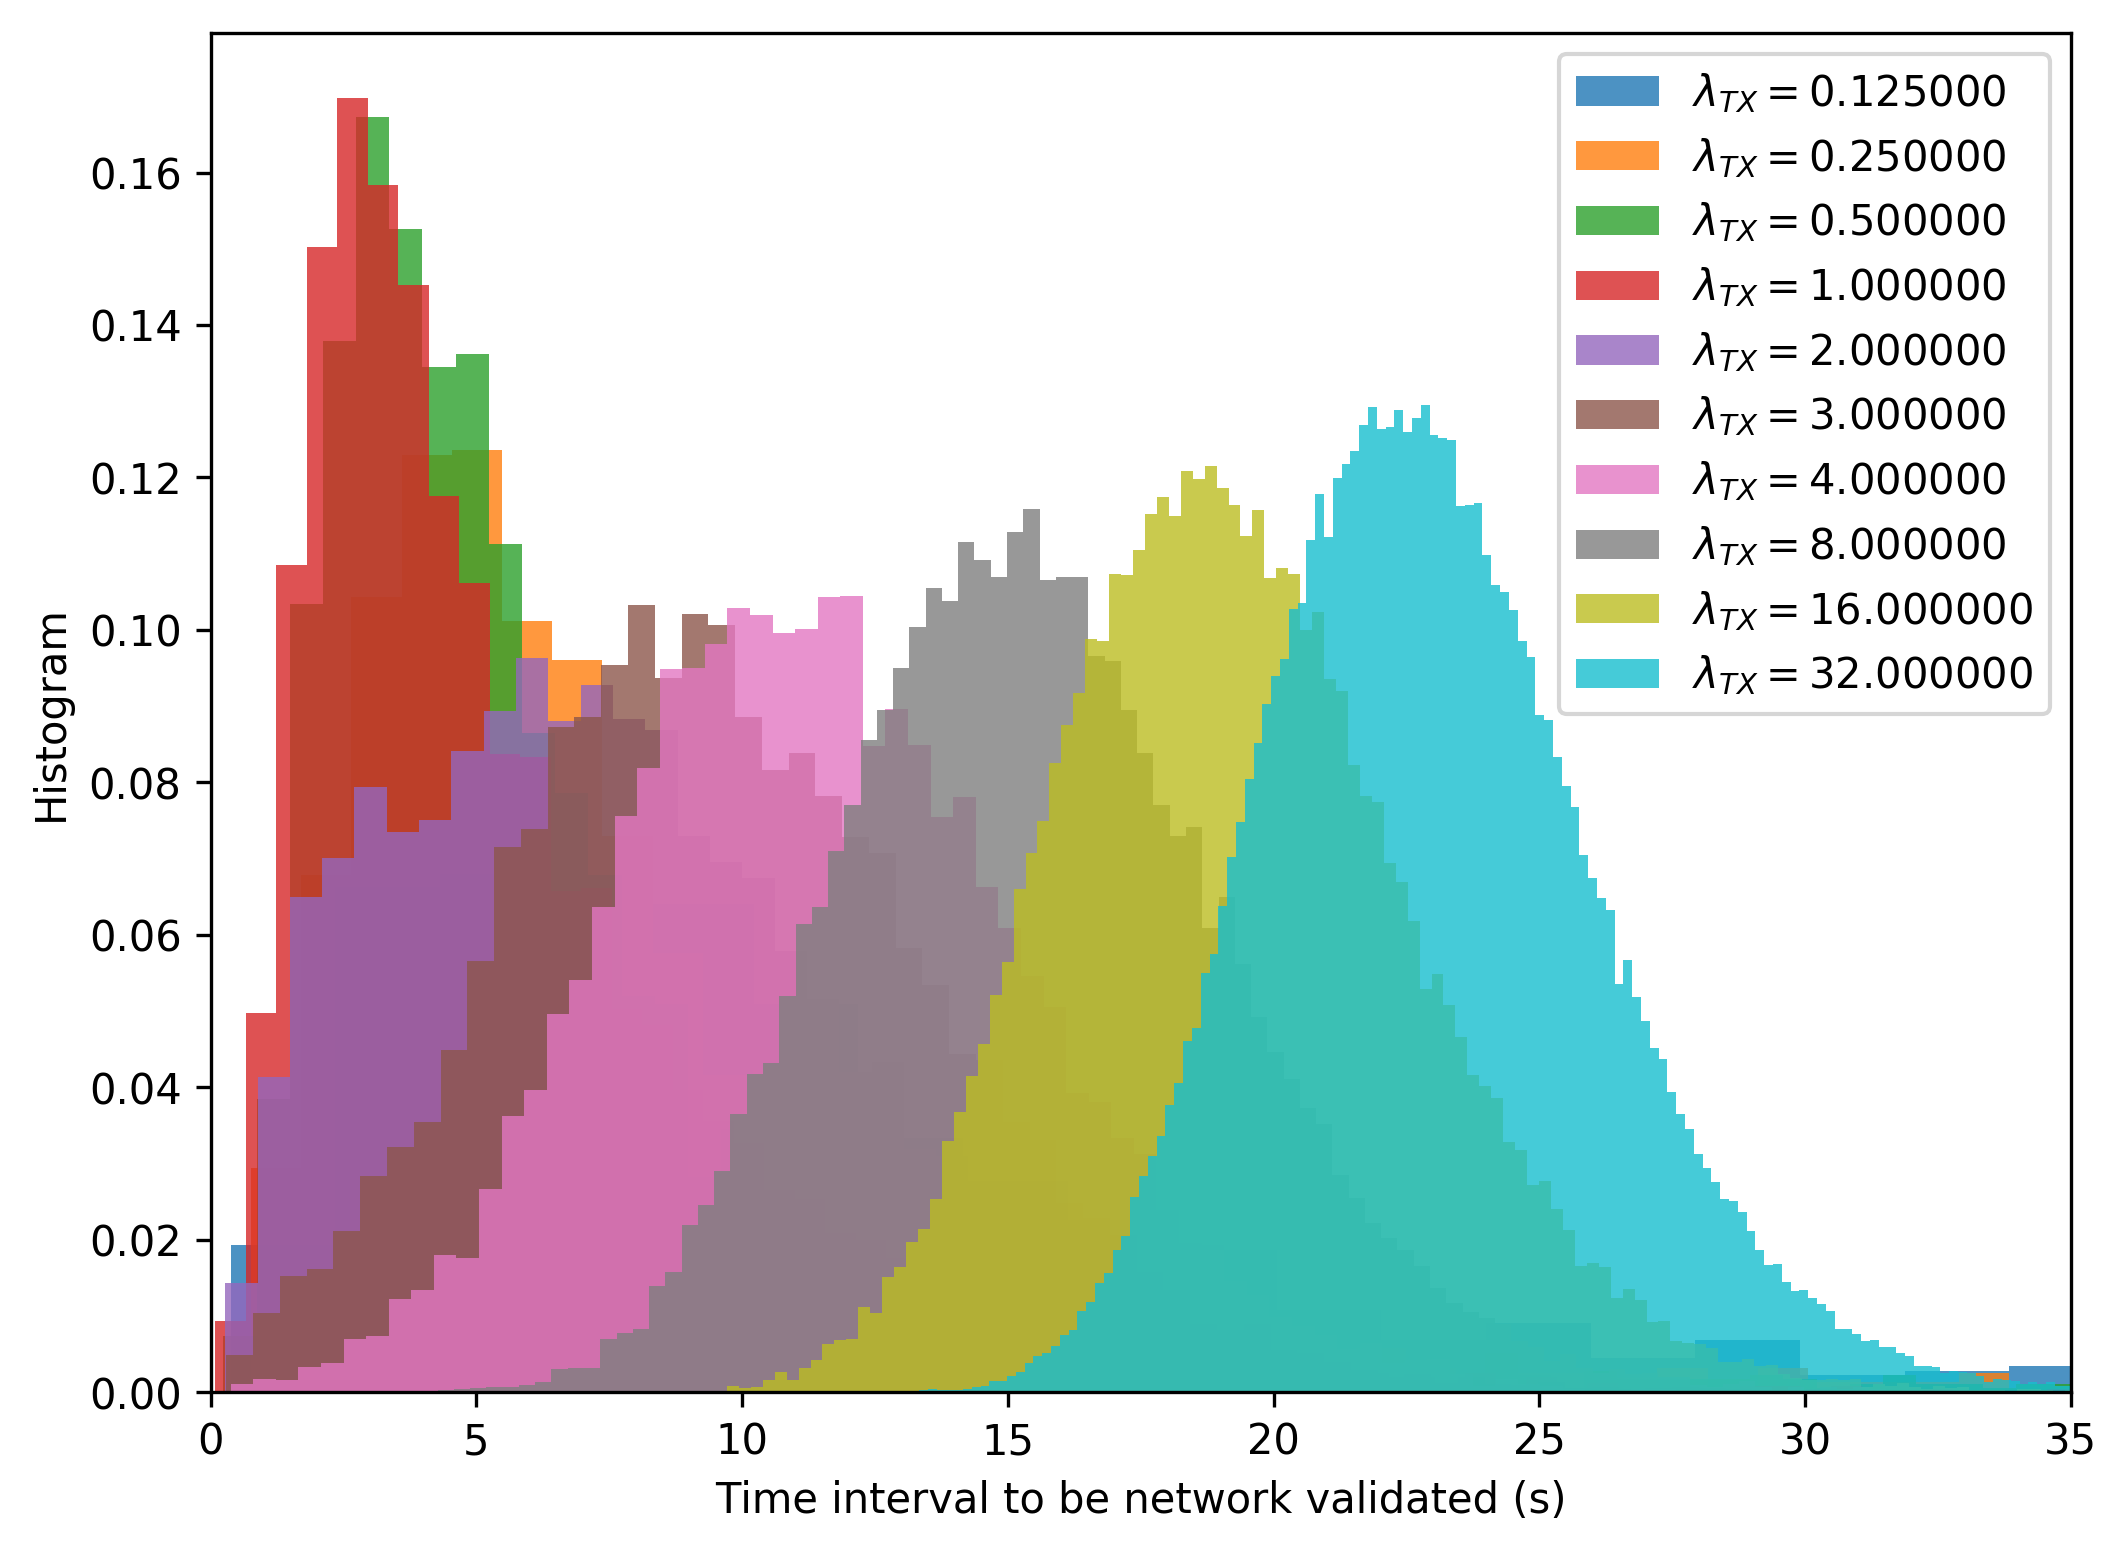
\includegraphics[width=\textwidth]{./images01/new2/nv_all.png}}

\subfloat[Only low load scenarios]{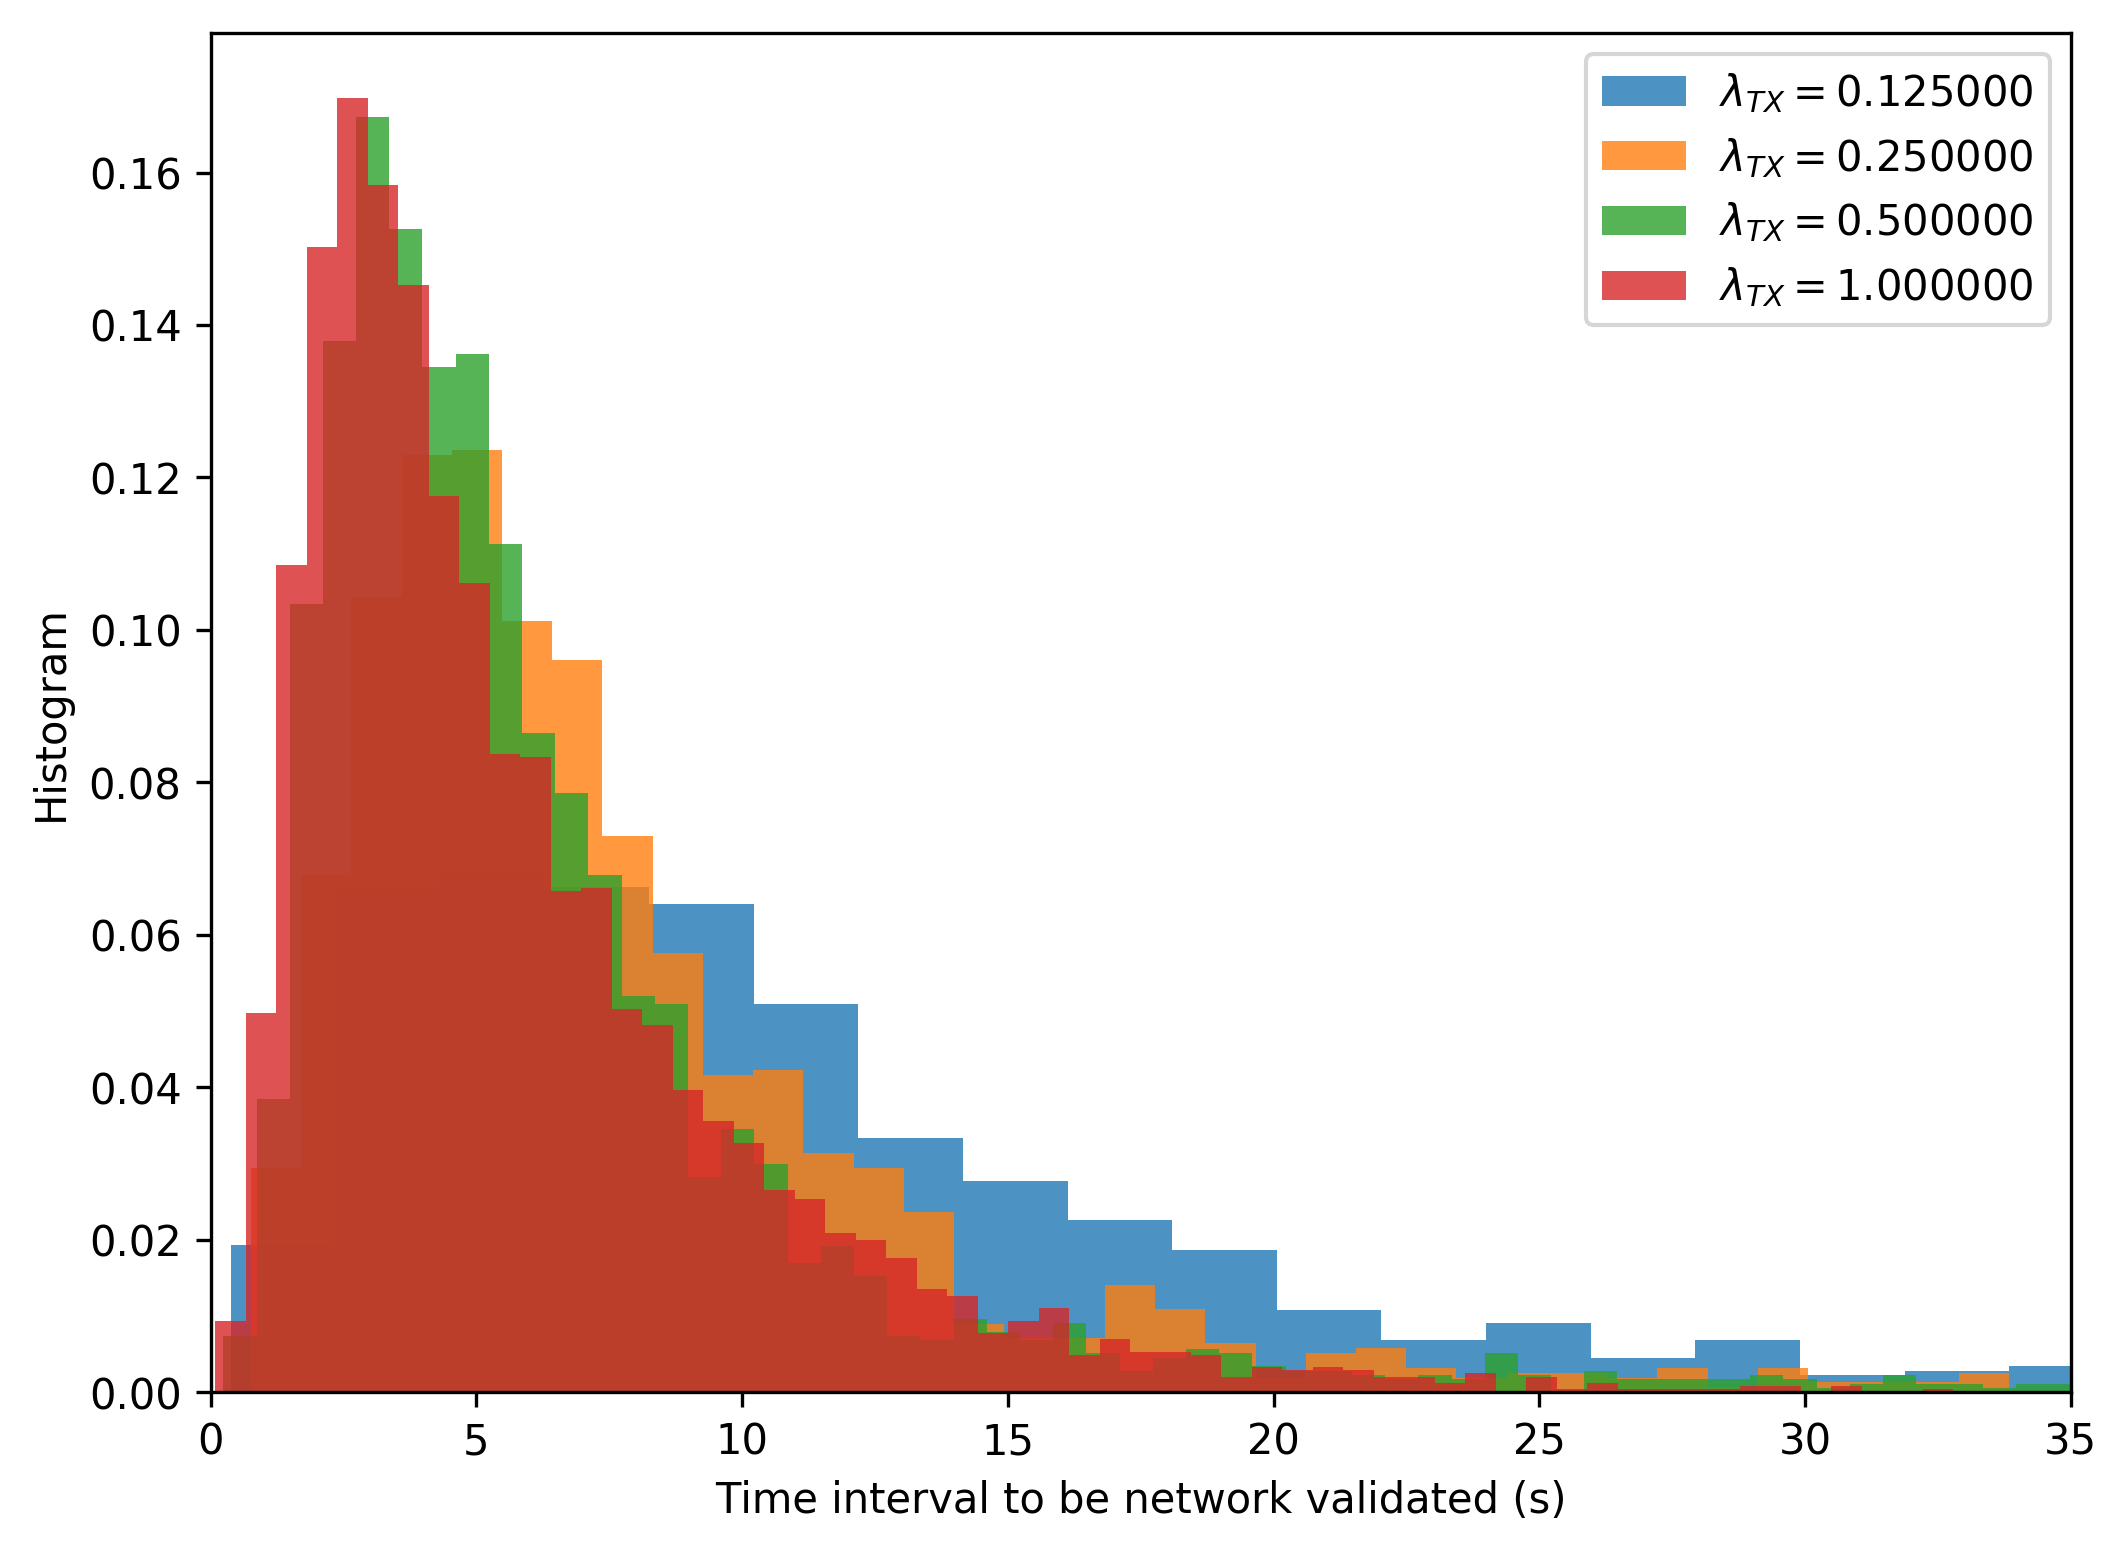
\includegraphics[width=\textwidth]{./images01/new2/nv_low.png}}

\caption{Histogram of the time it takes for a transaction to be network validated. A transaction is said to be network validated when all tips are confirming it directly or indirectly. \label{fig:hathor-network-validated}}
\end{figure}


%The number of transactions solving the proof-of-work may be modeled by a Birth and Death process, since if we have $k$ transactions solving the proof-of-work only two things may happen: either a new transaction will be created or one the transactions will finish solving the proof-of-work. Let the time between new transactions follows an exponential distribution with $\mu$ parameter, then the probability of a new transaction emerges before any transaction finishes its proof-of-work is $q_k = \mathbf{P}(T_{\text{new tx}} = \min\{T_{\text{new tx}}, T_1, T_2, \dots, T_k\}) = \frac{\mu}{\mu + \sum_{i=1}^k \lambda_i}$. Hence, the probability of any transaction finishes its proof-of-work before a new transaction emerges is $p_k = 1 - q_k = \frac{\sum_{i=1}^k \lambda_i}{\mu + \sum_{i=1}^k \lambda_i}$.

%\begin{theorem}
%\label{theorem-new-tx-not-tip}
%When a new transaction confirms an already confirmed transaction, the depth of all transactions remains the same, i.e., the depth of the transactions are only changed when a new transaction confirm an unconfirmed transaction.
%\end{theorem}

%\begin{theorem}
%The height of a transaction is equal to the maximum height of its parents plus one.
%\end{theorem}

%\begin{theorem}
%If new transactions choose randomly the unconfirmed transactions to be confirmed, then no unconfirmed transaction will be left behind, i.e., all transactions will be confirmed in due time.
%\end{theorem}

\chapter{Conclusion}

Bitcoin's underlying technology blockchain has been called by many as a major invention, even comparable to the invention of the internet. But it is unlikely that Bitcoin and blockchain have achieved the final or most optimal design for a secure and scalable electronic transaction system. In this work, I proposed and analysed a new architecture named Hathor, which seems a scalable alternative to Bitcoin.

Today, Bitcoin network can barely handle 8 transactions per second without increasing the unconfirmed transaction list to hundreds of thousands --- several transactions take days to be confirmed. In order to increase Bitcoin's capacity, its community has first proposed and implemented segregated witness, which improved scalability yet was not enough. Finally, they proposed the lightning network, which is in development and should be available in the next months. I believe these proposals relieve the network---a temporary solution---, but do not solve the scalability problem.

Hathor's architecture allows a great number of transactions per second, since new transactions confirm previous ones (and there is no such thing as ``maximum block size''). The more transactions are coming, the faster previous transactions will be confirmed. It is the opposite of Bitcoin because the network benefits from high volume scenarios. As I have shown, Hathor seems to solve the scalability problem present in Blockchain-based cryptocurrencies.

As the transactions also have a proof-of-work, it becomes harder to perform a spam attack. The attacker would spend a considerable amount of computational resources to solve the proof-of-work of every transaction, and the amount of work depends on the transaction's weight parameter. Future work may explore automatic adjustments in transaction's weight to improve spam prevention. For instance, the network can detect a higher number of new transactions coming and increase the transaction's weight for a while. Or else, the transaction's weight may be a function of the time between an output being spent and its spending transaction, so, transferring the same tokens over and over in a small window of time would require more work. Anyway, the transaction's weight seems to tackle the spam issue. The new challenge is to set a proper transaction's weight which would prevent spam without impairing IoT devices.

The last, but not least, challenge is the hashpower centralization. Although Bitcoin seems to have the most decentralized network among cryptocurrencies, there are few miners and mining pools which together control over 50\% of the network’s computing (hash)power \citep{gencer2018decentralization}. Hence, they have an oversized influence when it comes to changes in the Bitcoin protocol's behavior. Hathor's architecture splits the hashpower among miners and users. Even if miners have more individual hashpower than users, because they would have rigs with appropriate cooling and energy supply, I believe their aggregate hashpower will not surpass users' aggregate hashpower when millions of devices are generating transactions. Future IoT devices may even come with an application-specific integrated circuit (asic) designed to solve Hathor's proof-of-work without spending too much battery. Future work may check common IoT processors' hashpower, which would allows us to estimate how many devices would be necessary to surpass miners' hashpower.

Even though I have proposed to update block's weight every 24 hours (or 675 blocks), this was an arbitrary number. Future work may explore whether it would be feasible to continuously update block's weight, or what would be the optimal number of blocks between each update. I believe that the challenge of a continuous update approach would be preventing outdated nodes to discard valid blocks when two or more blocks were being propagated through Hathor's network. Maybe a solution would be allowing a range of block's weight instead of a single value, but future work would have to check whether this can be exploited by attackers.

I also presented a mathematical analysis of Blockchain, going though mining, hashpower change, orphan blocks, and double-spending attacks. Most of the presented results may directly be applied to Hathor's blocks, since their foundations are the same. As \citet{tangle2016} has already analyzed Tangle, I have just applied their results with a few extensions.

Future work may also further analyze other possibilities of attack in Hathor's network, such as malicious device not using random tip selection. Another major challenge affecting all cryptocurrencies is disk space use. How would one wipe out part of the blocks and transactions without putting security in risk? At first, all blocks and transactions are required to check whether anyone (including computer viruses) has tampered with transactions which had already been validated and stored in disk.


%- What is better: solves a PoW with $w$, or solves $n$ PoWs with $w/n$?

%\chapter{Proposal: Questions to be explored}

%Given these preliminaries, these are some questions with which we will be concerned.


%In this paper, we will analyze the network scaling and security. How a Hathor network scales, simulating different loads and measuring the bandwidth, computational effort, and storage space necessary to handle all the transactions in time. What is the minimum transaction's aggregated weight which it may be considered unlikely to be reversed?

%We are interested in how the rate of new transactions affects how long it takes to a new transaction to be confirmed for the first time. We had already run some simulations under normal load (Fig. \ref{fig-tangle-hist}) and high load (Fig. \ref{fig-tangle-hist-2}).

%\begin{figure}[ht]
%\centering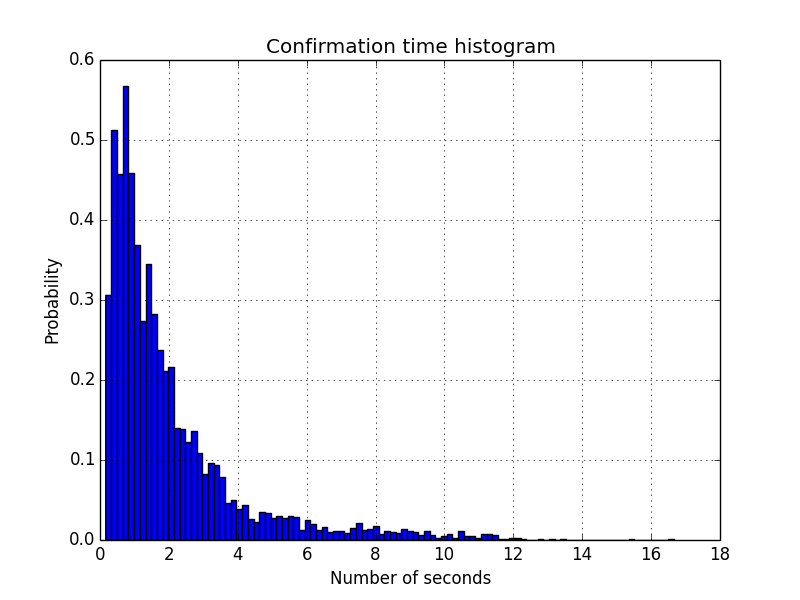
\includegraphics[width=\textwidth]{./images01/fig-tangle-hist.png}
%\caption{Histogram of how long has been a transaction waiting until its first confirmation. It was a simulation of 15 minutes with new transactions rate changing between 1 and 15 tx/s.\label{fig-tangle-hist}}
%\end{figure}

%\begin{figure}[ht]
%\centering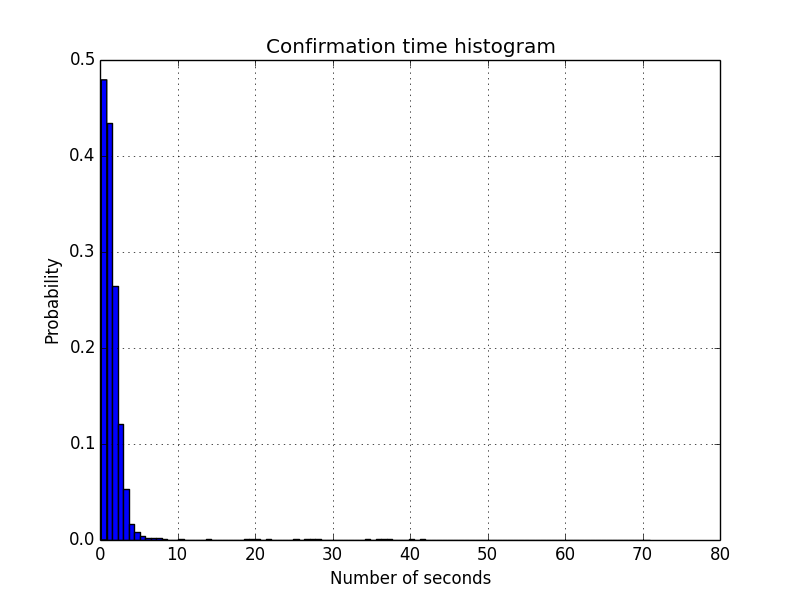
\includegraphics[width=\textwidth]{./images01/fig-tangle-hist-2.png}
%\caption{Histogram of how long has been a transaction waiting until its first confirmation. It was a simulation of 5 minutes with new transactions rate of 50 tx/s, i.e., very high load.\label{fig-tangle-hist-2}}
%\end{figure}


%Besides the time to the first confirmation, it is also important to measure how long it takes to a new transaction reach a specific accumulated weight. It is useful for exchanges and merchants to set their minimum requirements. Bitcoin's exchanges and merchants usually requires a minimum of 6 confirmations blocks.

%OLD \cite{tangle2016} suggests that constraining transactions' weight in a range would both prevent spam, because it would be necessary a minimum work to propagate a new transaction, and attacks, because an attacker would not be allowed to propagate a transaction with very high weight. We agree with the spam argument, and would like how a minimum weight would affect mobile devices's new transactions. We partially agree with the upper bound, because an attacker would be able to generate many transaction with lower weight. We will analyze if constraining transactions' weight would be effective against nuclear submarine attacks.

%OLD We have another suggestion to prevent nuclear submarine attacks: set a maximum depth for the transactions confirmed by a new transaction. So, new transactions would have to confirming newer transactions instead of old transactions, and a nuclear submarine attack would be controlled because the attacker would be not be able to create a large separate DAG. But the maximum depth rule would possibly also affect transaction created by low (hash)power devices, because it would take a longer time to solve the proof-of-work and, if the confirmations are going fast, the transaction would possibly be invalidated. This raises another important question: what would be an optimal maximum depth allowed?

%OLD If we would like to include fee transactions, how would it be distributed between confirmations? As transactions may have multiple direct confirmations, it is not obvious who would receive the transaction fee. An intuitive suggestion would be to give the fee to the first confirmation with a minimum weight, but it might have some propagation problems, because it takes a while to propagate a transaction in the network and there would be conflict.

%OLD In order to solve the fee distribution problem, we will simulate how the network would behave if we include blocks. These blocks would be like Bitcoin's, with an adjustable proof-of-work according to the network's hashpower. They would receive the fees from all confirmed transactions which had not been confirmed by any block before, and they would be able to generate new coins. These blocks would also help solving other problems.

%\begin{enumerate}
%\item Which parameters turns the network more or less vulnerable to attacks?
%\item Is there an optimal strategy to attack?
%\item Could new coins be generated demanding a proof-of-work with dynamic difficulty, like in Bitcoin?
%\item What is the equation of number of tips over time? What is the equation of how long it takes to a transaction to be confirmed for the first time? What is the equation of the accumulated weight of a transaction over time? Some equations have already been proposed by \citet{tangle2016}.
%\end{enumerate}

%\cleardoublepage
 
%\ctparttext{Oie}
 
\part{An invitation to Sparse Distributed Memory: from the theoretical model to the system dynamics}
% !TEX root = ../partial-sdm.tex

\chapter{Introduction}

Sparse Distributed Memory (SDM) \citep{Kanerva1988} is a mathematical model of long-term memory that has a number of neuroscientific and psychologically plausible dynamics. Such model may be applied in all sort of applications because it would replicate human capacity to remember past experiences from clues of the present. For instance, when one is walking on a dark alley and is afraid of something, one cannot explain where ones fear come from. They just feel it. We may interpret this situation as clues of the present --- a dark alley --- recalling past experiences from memory and thus generating the scared feeling. Our memory is able to make a parallel between previous experiences and the clues. Although one has never been in the exactly same situation, ones brain makes an analogy and recognizes the danger. This flexibility into mapping one situation in another is an important human feature which is hard to replicate into computers.

It has been applied in many different fields, like pattern recognition \citep{norman2003modeling, rao1995natural}, noise reduction \citep{Meng2009}, handwriting recognition \citep{fan1997genetic}, robot automation \citep{Rajesh1998, mendes2008robot}, and so forth. \cite{Linhares2011} has showed that SDM respects the limits of short-term memory discussed by \citet{Miller1995} and \citet{Cowan2011}. Despite all those applications, there is not a reference implementation which would allow one to replicate the results published in a paper, to check the source code for details, and to improve it. Thus, even though intriguing results have been achieved using SDM, it requires great effort of researchers to improve someone's work.

It is our belief that such a tool could bring orders of magnitude more researchers and attention if they were able to use the model, at zero cost, with an easy to use high-level language such as python in an intuitive platform such as juypyter notebook. Neuroscientists interested in long-term memory storage should not have to worry about high-bandwidth vector parallel computation.  This new tool provides a ready to use system in which experiments can be executed almost as soon as they are designed and it may accelerate researches \citep{shen2014interactive}.

Our motivation was our own effort in order to run our models. As there is no reference implementation, we had to implement our own and run several simulations to ensure that our implementation was correct and bug free. Thus, we had to deviate from our main goal --- which was to test our models --- and to focus in the implementation itself. Furthermore, new members in our research group had to go through different source codes developed by former members.

Extensions of SDM has been used in many applications. For example, \citet{Snaider2011} extended SDM to efficiently store sequences of vectors and trees.  \citet{Rajesh1998} used a modified SDM in an autonomous robot. \citet{Meng2009} modified SDM to clean patterns from noisy inputs. \citet{fan1997genetic} extended SDM with genetic algorithms. \citet{chada2016you} extended SDM creating the Rotational Sparse Distributed Memory (RSDM), which is used to modeling network motifs, dynamic flexibility, and hierarchical organization, all results from neuroscience literature.

The main contribution of this work is a reference implementation which yields (i) orders of magnitude gains in performance, (ii) has several backends and operations, (iii) has been validated against the mathematical model, (iv) is cross-platform, and (v) is easily extended to fulfill other research models. Our reference implementation may, hopefully, accelerate research into the model's dynamics and make it easier for readers to replicate any previous results and easily understand the source-code of the model.  Moreover, it is compatible with jupyter notebook and researchers may share their notebooks possibly accelerating the advances in their fields \citep{shen2014interactive}.

Other contributions have also been introduced, which include (i) a noise filtering approach, (ii) a supervised classification algorithm, (iii) and a reinforcement learning algorithm, all of them using only the original SDM proposed by Kanerva, i.e., with no additional mechanisms, algorithms, data structures, etc. Although some of our applications have already been explored in previous work \citep{Meng2009, fan1997genetic, rao1995natural}, all of them have done some adapting of SDM to their problems, and none of them have used just the ideas introduced by Kanerva. We have presented different approaches with no adaptations at all.

Finally, we have found an anomaly in one of Kanerva's prediction, which we believe is related to SDM capacity. We have also tested a generic reading operation proposed by professor Paulo Murilo (personal communication).

\chapter{Notation}

\begin{tabular}{cp{\textwidth}}
  $n$ & Number of dimensions, i.e., $n=1,000$. \\
  $N$ & Size of the binary space --- $|\{0, 1\}^n| = 2^n$. \\
  $N'$ & Number of hard-locations samples from $\{0, 1\}^n$. Its typical value is 1,000,000, as suggested by \citet{Kanerva1988}. \\
  $H$ & Same as $N'$. \\
  $r$ & Access radius, i.e., when $n=1,000$ and $N'=1,000,000$, its typical value is $451$. This value is calculated to activate, on average, one thousand of $N'$. \\
  $\eta$ & A bitstring, usually a datum. \\
  $\eta_x$ & A clue $x$ bits away from $\eta$, i.e., $\text{dist}(\eta, \eta_x) = x$. \\
  $\xi$ & A bitstring, usually an address. \\
  $\text{dist}(x, y)$ & Hamming distance between $x$ and $y$ \\
  $\text{d}(x, y)$ & Same as $\text{dist}(x, y)$
\end{tabular}\\

\chapter{Sparse Distributed Memory}

% !TEX root = ../partial-sdm.tex

Sparse Distributed Memory (SDM) is a mathematical model for cognitive memory published by \citet{Kanerva1988}. It introduces many interesting mathematical properties of $n$-dimensional binary space that, in a memory model, are psychologically plausible.  Most notable among these are the tip-of-the-tongue phenomenon, conformity to Miller's magic number \citep{Linhares2011} and robustness against loss of neurons.

The data and address space belong to binary space and are represented by a sequence of bits, called bitstrings. The distance between two bitstrings is calculated using the Hamming distance. It is defined for two bitstrings of equal length as the number of positions at which the bits are different. For example, $00110_{b}$ and $01100_{b}$ are bitstrings of length 5 and their Hamming distance is 2. One has to be careful when thinking intuitively about distance in SDM because the Hamming distance does not have the same properties of, say, the Euclidean distance.

\begin{figure}[p!]
  \centering
  \subfloat[$Q_3$]{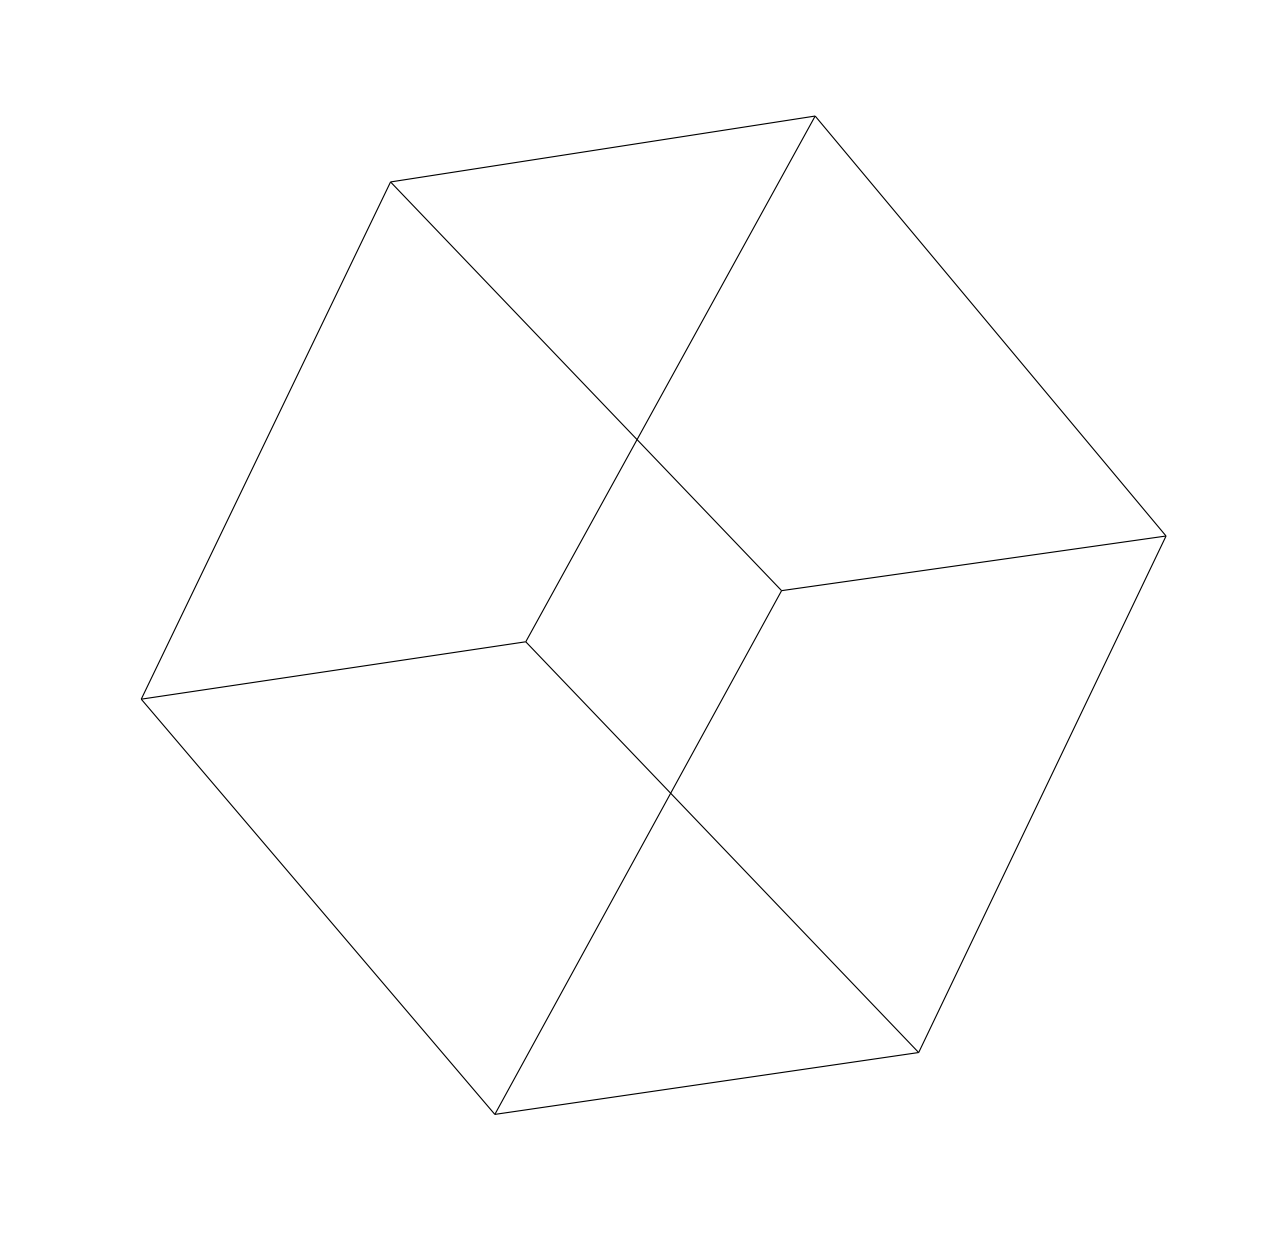
\includegraphics[width=2.2in]{./images02/new-images/qn3.png}}
  \subfloat[$Q_7$]{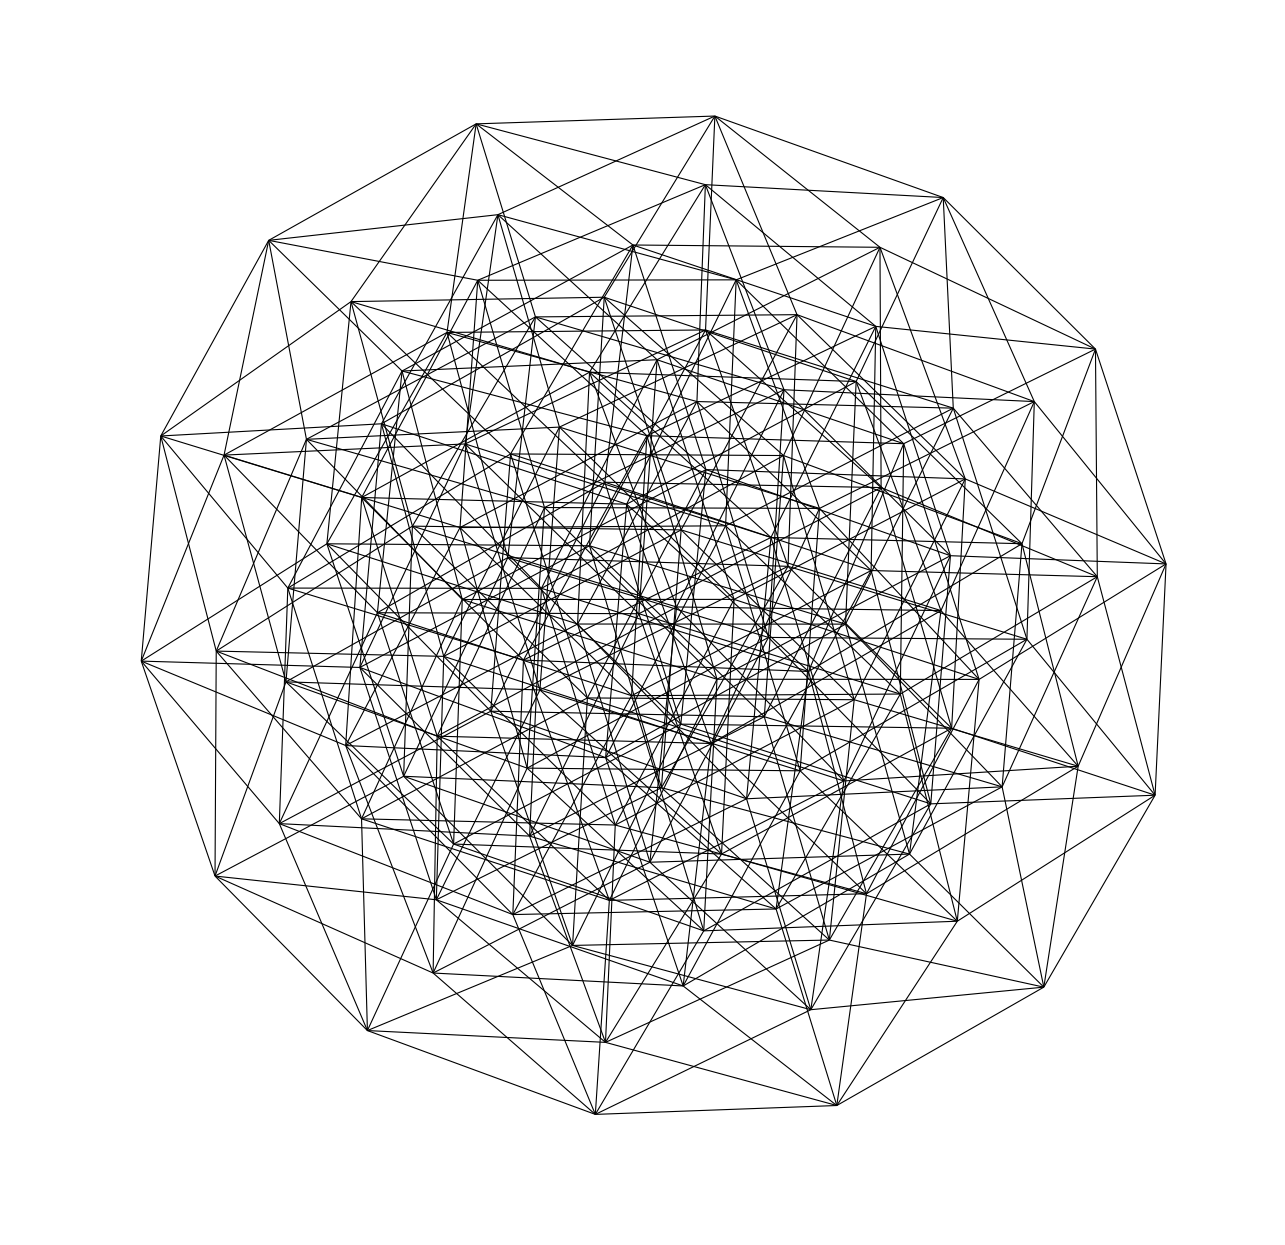
\includegraphics[width=2.2in]{./images02/new-images/qn7.png}}

  \subfloat[$Q_{10}$]{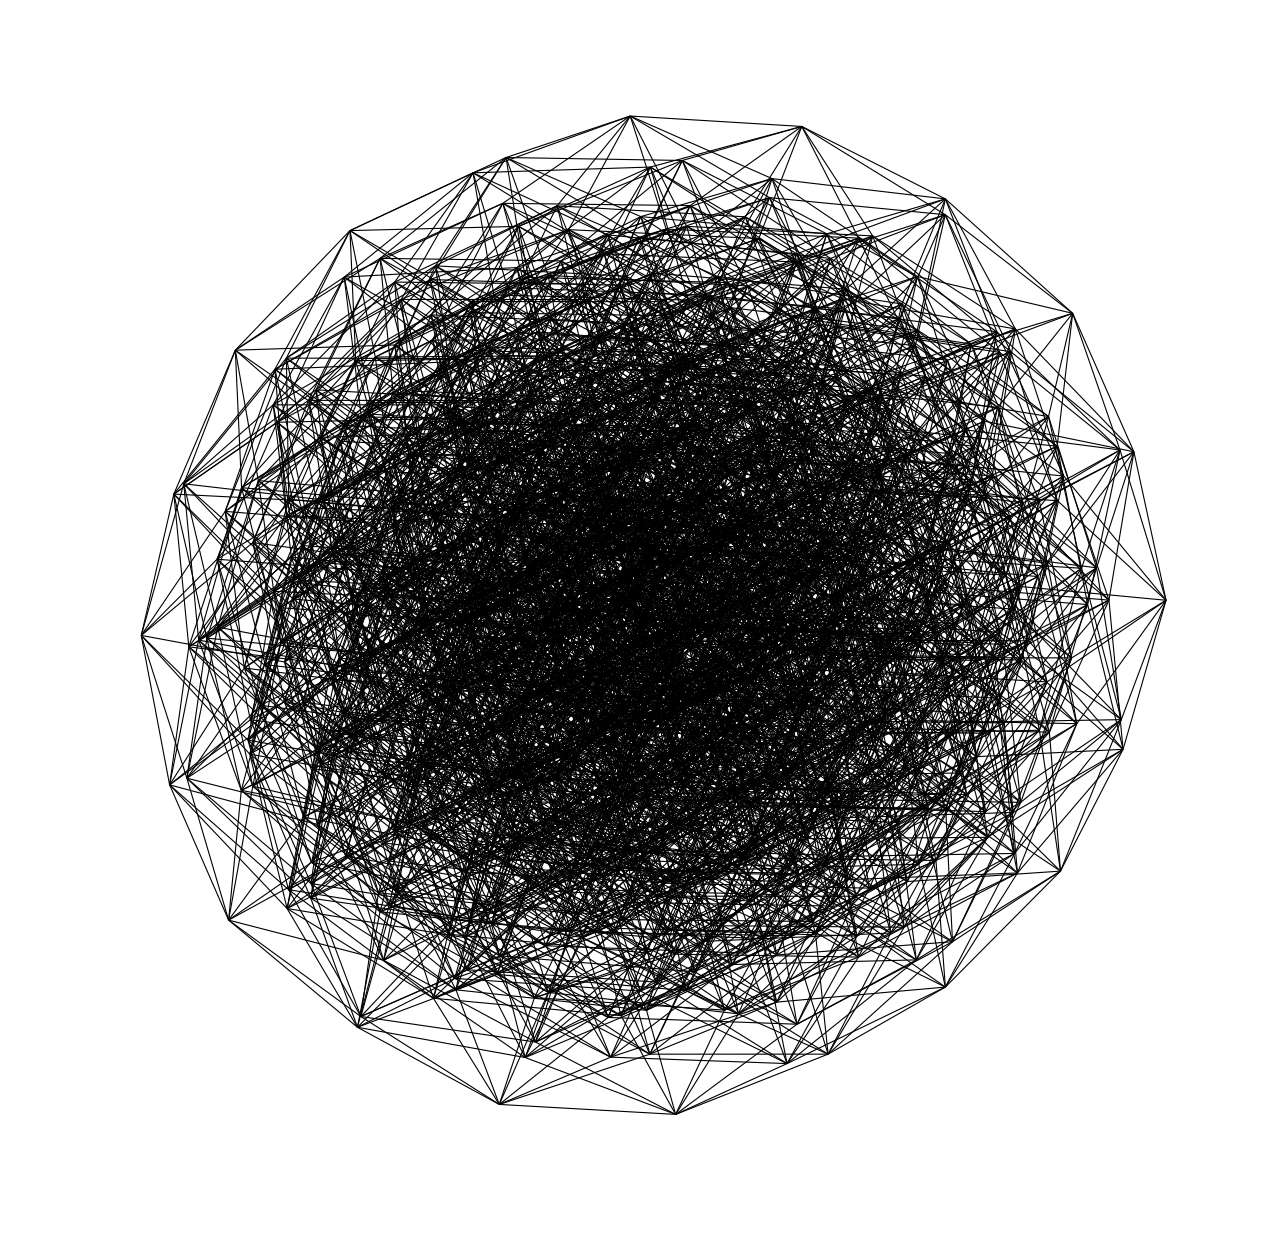
\includegraphics[width=4.0in]{./images02/new-images/qn10.png}}
  \caption{Here we have $Q_n$, for $n \in$ \{3, 7, 10\}. Each node represents a possible bitstring in $\{0,1\}^n$, and two nodes are linked if the bitstrings differ by a single dimension.  A number of observations can be made here. First, the number of nodes grows as $2^n$ as $n$ grows; which makes use of the entire space infeasible as $n>>20$. Another interesting observation, better seen in the figures below, is that most of the space lies at the center, at a distance of around 500 from any given vantage point.\label{hypercubes}}
\end{figure}



The graph composed of $\{0,1\}^n$ nodes and links between nodes $iff$ their Hamming distance is one is called the \emph{hypercube graph}, or $Q_n$, as in Figure \ref{hypercubes}.  Though Kanerva has derived many combinatorial properties of the space, I believe that this is a aesthetically appealing object on its own, and beautiful results can be found in the graph-theoretical literature. A good survey is found in \citet{harary1988survey}.


Here is an interesting question that I leave for further research: A hypercube with n dimensions can be divided by two hypercubes with $n-1$ dimensions. Is there an algorithm that separates the area of each hard-location in such a form that there exists a function mapping each bitstring in $\{0,1\}^n$ to the set of hard locations it belongs to?  In other words… though this would break Kanerva's assumption of a uniformly distributed set of hard locations for a perfectly symmetrical set of hard locations, there could be large performance gains if such a mapping function from a bitstring to its corresponding set of nearest hard locations exists.





Unlike traditional memory used by computers, SDM performs read and write operations in a multitude of addresses, also called neurons.  That is, the data is not written, or it is not read in a single address spot, but in many addresses. These are called activated addresses, or activated neurons.

The activation of addresses takes place according to their distances from the datum. Suppose one is writing datum $\eta$ at address $\xi$, then all addresses inside a circle with center $\xi$ and radius $r$ are activated. So, $\eta$ will be stored in all these activated addresses, which are around address $\xi$, such as in Figure \ref{fig-addresses-inside-access-radius}.  An address $\xi'$ is inside the circle if its hamming distance to the center $\xi$ is less than or equal to the radius $r$, i.e. $distance(\xi,\xi')\leq r$.

\begin{figure}[!htb]
\centering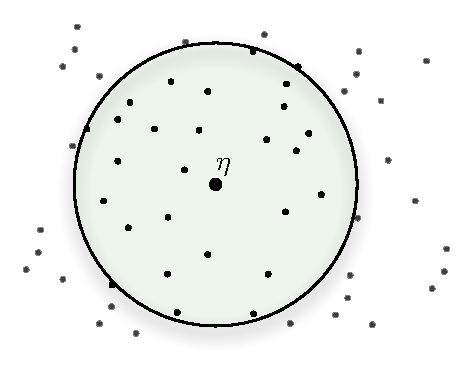
\includegraphics[scale=0.75]{./images02/p_circle_r.pdf}

\caption{Activated addresses inside access \protect \\
radius $r$ around center address.\label{fig-addresses-inside-access-radius}}
\end{figure}



Every time write or read in SDM memory activates a number of addresses with close distance.  The data is written in these activated addresses or read from them.  These issues will be addressed in due detail further on, but a major difference from a traditional computer memory is that the data are always stored and retrieved in a multitude of addresses. This way SDM memory has robustness against loss of addresses (e.g., death of a neuron).

In traditional memory, each datum is stored in an address and every look up of a specific datum requires a search through the memory. In spite of computer scientists having developed beautiful algorithms to perform fast searches, almost all of them do a precise search. That is, if you have an imprecise clue of what you need, these algorithms will simply fail.

In SDM, the data space is the same as the address space, which amounts to a vectorial, binary space, that is, a $\{0,1\}^{n}$ space. This way, the addresses where the data will be written are the same as the data themselves. For example, the datum $\eta=00101_{b}\in\{0,1\}^{5}$ will be written to the address $\xi=\eta=00101_{b}$. If one chooses a radius of 1, the SDM will activate all addresses one bit away or less from the center address. So, the datum $00101_{b}$ will be written to the addresses $00101_{b}$, $10101_{b}$, $01101_{b}$, $00001_{b}$, $00111_{b}$, and $00100_{b}$.

In this case, when one needs to retrieve the data, one could have an imprecise cue at most one bit away from $\eta$, since all addresses one bit away have $\eta$ stored in themselves.  Extending this train of thought for larger dimensions and radius, exponential numbers of addresses are activated and one can see why SDM is a distributed memory.

When reading a cue $\eta_{x}$ that is $x$ bits away of $\eta$, the cue shares many addresses with $\eta$. The number of shared addresses decreases as the cue's distance to $\eta$ increases, in other words, as $x$ increases. This is shown in Figure \ref{fig-shared-addresses}.  The target datum $\eta$ was written in all shared addresses, thus they will bias the read output in the direction of $\eta$. If the cue is sufficiently near the target datum $\eta$, the read output will be closer to $\eta$ than $\eta_{x}$ was. Repeating the read operation increasingly gets results closer to $\eta$, until it is exactly the same. So, it may be necessary to perform more than one read operation in order to converge to the target data $\eta$.

\begin{figure}[!htb]
\centering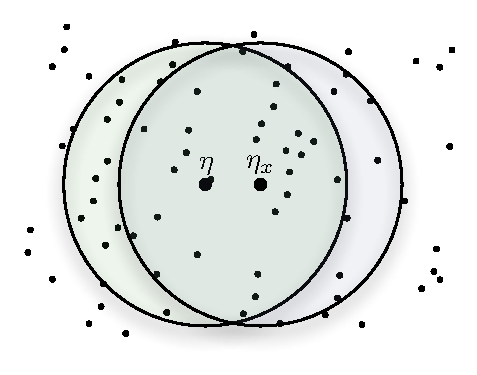
\includegraphics[scale=0.75]{./images02/p1_inter_p2.pdf}

\caption{Shared addresses between the \protect \\
target datum $\eta$ and the cue $\eta_{x}$. \label{fig-shared-addresses}}
\end{figure}


The addresses of the $\{0,1\}^{n}$ space grows exponentially with the number of dimensions $n$, i.e. $N=2^{n}$. For $n=100$ we have $N\approx10^{30}$, which is incredibly large when related to a computer memory. Furthermore, \citet{Kanerva1988} suggests $n$ between 100 and 10,000. Recently he has postulated 10,000 as a desirable minimum $N$ (personal communication). To solve the feasibility problem of implementing this memory, Kanerva made a random sample of $\{0,1\}^{n}$, in his work, having $N'$ elements. All these addresses in the sample are called hard-locations. Other elements of $\{0,1\}^{n}$, not in $N'$, are called virtual neurons. This is represented in Figure \ref{fig-hardlocations}.  All properties of read and write operations presented before remain valid, but limited to hard-locations. Kanerva suggests taking a sample of about one million hard-locations.

Using this sample of binary space, our data space does not exist completely.  That is, the binary space has $2^{n}$ addresses, but the memory is far away from having these addresses available. In fact, only a fraction of this vectorial space is actually instantiated. Following Kanerva's suggestion of one million hard-locations, for $n=100$, only $100\cdot10^{6}/2^{100}=7\cdot10^{-23}$ percent of the whole space exists, and for $n=1,000$ only $100\cdot10^{6}/2^{1000}=7\cdot10^{-294}$ percent.

Kanerva also suggests the selection of a radius that will activate, on average, one one thousandth of the sample, which is 1,000 hard-locations for a sample of one million addresses. In order to achieve his suggestion, a 1,000-dimension memory uses an access radius $r=451$, and a 256-dimensional memory, $r=103$. We think that a 256-dimensional memory may be important because it presents conformity to Miller's magic number \citep{Linhares2011}.

\begin{figure}[!htb]
\centering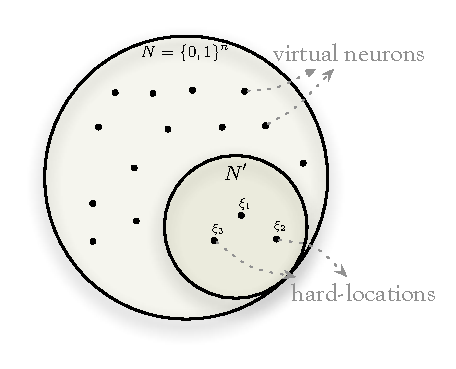
\includegraphics[scale=0.75]{./images02/hardlocations.pdf}

\caption{Hard-locations randomly sampled from binary space.\label{fig-hardlocations}}
\end{figure}


Since a cue $\eta_{x}$ near the target bitstring $\eta$ shares many hard-locations with $\eta$, SDM can retrieve data from imprecise cues. Despite this feature, it is very important to know how imprecise this cue could be while still giving accurate results. What is the maximum distance from our cue to the original data that still retrieves the right answer? An interesting approach is to perform a read operation with a cue $\eta_{x}$, that is $x$ bits away from the target $\eta$.  Then measure the distance from the read output and $\eta$. If this distance is smaller than $x$ we are converging. Convergence is simple to handle, just read again and again, until it converges to the target $\eta$. If this distance is greater than $x$ we are diverging. Finally, if this distance equals $x$ we are in a tip-of-the-tongue process.  A tip-of-the-tongue psychologically happens when you know that you know, but you can't say what exactly it is. In SDM mathematical model, a tip-of-the-tongue process takes infinite time to converge. \citet{Kanerva1988} called this $x$ distance, where the read's output averages $x$, the critical distance. Intuitively, it is the distance from which smaller distances converge and greater distances diverge. In Figure \ref{fig-p1-p2-iterative-read}, the circle has radius equal to the critical distance and every $\eta_{x}$ inside the circle should converge.  The figure also shows a convergence in four readings.

\begin{figure}[!htb]
\centering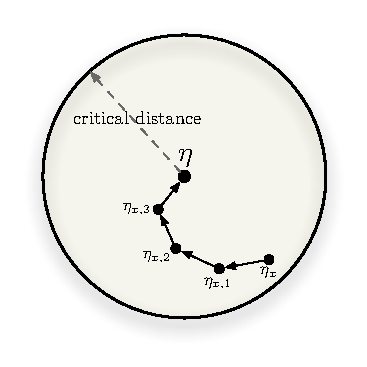
\includegraphics[scale=0.75]{./images02/p1_p2_iter_read.pdf}

\caption{In this example, four iterative readings were\protect \\
required to converge from $\eta_{x}$ to $\eta$.\label{fig-p1-p2-iterative-read}}
\end{figure}


The $\{0,1\}^{n}$ space has $N=2^{n}$ locations from which we instantiate $N'$ samples. Each location in our sample is called a hard-location.  On these hard-locations we do operations of read and write. One of the insights of SDM is exactly the way we read and write: using data as addresses in a distributed fashion. Each datum $\eta$ is written in every activated hard-location inside the access radius centered on the address, that equals datum, $\xi=\eta$. Kanerva suggested using an access radius $r$ having about one one thousandth of $N'$.  As an imprecise cue $\eta_{x}$ shares hard-locations with the target bitstring $\eta,$ it is possible to retrieve $\eta$ correctly. (Actually, probably more than one read is necessary to retrieve exactly $\eta.)$.  Moreover, if some neurons are lost, only a fraction of the datum is lost and it is possible that the memory can still retrieve the right datum.

A random bitstring is generated with equal probability of $0$'s and $1$'s in each bit. One can readily see that the average distance between two random bitstrings has binomial distribution with mean $n/2$ and standard deviation $\sqrt{n/4}$. For a large $n$, most of the space lies close to the mean and has fewer shared hard-locations.  As two bitstrings with distance far from $n/2$ are very improbable, \citet{Kanerva1988} defined that two bitstrings are orthogonal when their distance is $n/2$.

The write operation needs to store, for each dimension bit which happened more ($0$'s or $1$'s). This way, each hard-location has $n$ counters, one for each dimension. The counter is incremented for each bit $1$ and decremented for each bit $0$. Thus, if the counter is positive, there have been more $1$'s than $0$'s, if the counter is negative, there have been more $0$'s than $1$'s, and if the counter is zero, there have been an equal number of $1$'s and $0$'s. Table \ref{tab:write operation} shows an example of a write operation being performed in a 7-dimensional memory.

\begin{table}
\begin{tabular}{c|c|c|c|c|c|c|c|}
\cline{2-8}
$\eta$ & 0 & 1 & 1 & 0 & 1 & 0 & 0\tabularnewline
\cline{2-8}
$\xi_{\textit{before}}$ & 6 & -3 & 12 & -1 & 0 & 2 & 4\tabularnewline
\cline{2-8}
\multicolumn{1}{c}{} & \multicolumn{1}{c}{\textcolor{red}{\small{}$\Downarrow$ -1}} & \multicolumn{1}{c}{\textcolor{red}{\small{}$\Downarrow$ +1}} & \multicolumn{1}{c}{\textcolor{red}{\small{}$\Downarrow$ +1}} & \multicolumn{1}{c}{\textcolor{red}{\small{}$\Downarrow$ -1}} & \multicolumn{1}{c}{\textcolor{red}{\small{}$\Downarrow$ +1}} & \multicolumn{1}{c}{\textcolor{red}{\small{}$\Downarrow$ -1}} & \multicolumn{1}{c}{\textcolor{red}{\small{}$\Downarrow$ -1}}\tabularnewline
\cline{2-8}
$\xi_{\textit{\textit{after}}}$ & \textbf{5} & \textbf{-2} & \textbf{13} & \textbf{-2} & \textbf{1} & \textbf{1} & \textbf{3}\tabularnewline
\cline{2-8}
\end{tabular}

\caption{Write operation example in a 7-dimensional memory of data $\eta$
being written to $\xi$, one of the activated addresses.\label{tab:write operation}}


\end{table}


The read is performed polling each activated hard-location and statistically choosing the most written bit for each dimension. It consists of adding all $n$ counters from the activated hard-locations and, for each bit, choosing bit 1 if the counter is positive, choose bit 0 if the counter if negative, and randomly choose bit 0 or 1 if the counter is zero.


\section{Neurons as pointers}

One interesting view is that neurons in SDM work like pointers. As we write bitstrings in memory, the hard-locations' counters are updated and some bits are flipped. Thus, the activated hard-locations do not necessarily point individually to the bitstring that activated it, but together they point correctly. In other words, the read operation depends on many hard-locations to be successful. This effect is represented in Figure \ref{fig-p1-pointers}: where all hard-locations inside the circle are activated and they, individually, do not point to $\eta$.  But, like vectors, adding them up points to $\eta$. If another datum $\nu$ is written into the memory near $\eta$, the shared hard-locations will have information from both of them and would not point to either.  All hard-locations outside of the circle are also pointing somewhere (possibly other data points). This is not shown, however, in order to keep the picture clean and easily understandable.

\begin{figure}[!htb]
\centering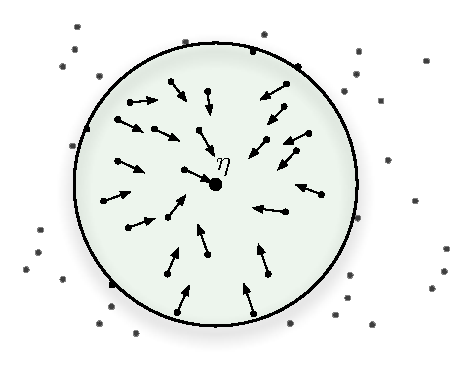
\includegraphics[scale=0.75]{./images02/p1_after_write.pdf}

\caption{Hard-locations pointing, approximately, to the target bitstring.\label{fig-p1-pointers}}
\end{figure}



\section{Concepts}

Although Kanerva does not mention concepts directly in his book \citep{Kanerva1988}, the author's interpretation is that each bitstring may be mapped to a concept. Thus, unrelated concepts are orthogonal and concepts could be linked through a bitstring near both of them. For example, ``beauty'' and ``woman'' have distance $n/2$, but a bitstring that means ``beautiful woman'' could have distance $n/4$ to both of them. As a bitstring with distance $n/4$ is very improbable, it is linking those concepts together. \citet{Linhares2011} approached this concept via ``chunking through averaging''.

Due to the distribution of hard-locations between two random bitstrings, the vast majority of concepts is orthogonal to all others. Consider a non-scientific survey during a cognitive science seminar, where students asked to mention ideas unrelated to the course brought up terms like birthdays, boots, dinosaurs, fever, executive order, x-rays, and so on. Not only are the items unrelated to cognitive science, the topic of the seminar, but they are also unrelated to each other.

For any two memory items, one can readily find a stream of thought relating two such items (``Darwin gave dinosaurs the boot''; ``she ran a fever on her birthday''; ``isn't it time for the Supreme Court to x-ray that executive order?'', ... and so forth). Robert French presents an intriguing example in which one suddenly creates a representation linking the otherwise unrelated concepts of ``coffee cups'' and ``old elephants'' \citep{French1997}.

This mapping from concepts to bitstrings brings us two main questions: (i) Suppose we have a bitstring that is linking two major concepts.  How do we know which concepts are linked together? (ii) From a concept bitstring how can we list all concepts that are somehow linked to it? This second question is called the problem of spreading activation.


\section{Read operation}

In his work, Kanerva proposed and analyzed a read algorithm called here Kanerva's read. His read takes all activated hard-locations counters and sum them. The resulting bitstring has bit $1$ where the result is positive, bit $0$ where the result is negative, and a random bit where the result is zero. In a word, each bit is chosen according to all written bitstrings in all hard-locations, being equal to the bit more appeared. Table \ref{tab:kanerva-read} shows an example of Kanerva's read result bitstring.

Daniel Chada, one member of our research group, proposed another way to read in SDM, in this work called Chada's read. Instead of summing all hard-location counters, each hard-location evaluates its resulting bitstring individually. Then, all resulting bitstrings are summed again, and the same rule as Kanerva applies. Table \ref{tab:chada-read} shows an example of Chada's read result bitstring. The counter's values are normalized to 1, for positive ones, or -1, for negative ones, and the original values are the same as in Table \ref{tab:kanerva-read}.

The main change between Kanerva's read and Chada's read is that, in the former, a hard-location that has more bitstrings written has a greater weight in the decision of each bit. In the latter, all hard-locations have the same weight, because they can contribute to the sum with only one bitstring.

A member of my Master's committee, professor Paulo Murilo, has proposed a generalized reading operation (personal communication), which covers both Kanerva's and Chada's read --- and opens a new venue of potential discoveries. He proposed summing all hard-location counters raised to the power of $z$ while holding the original sign of the counter (positive or negative). Thus, Kanerva's read would be the same as $z=1$, while Chada's would be the same as $z=0$. Hence, we will here explore how SDM would behave with other values of $z$, such as 0.5, 2, and 3.

\begin{table}
\begin{minipage}[t]{0.5\columnwidth}%
\subfloat[Kanerva's read example\label{tab:kanerva-read}]{%
\begin{tabular}{c|c|c|c|c|c|}
\cline{2-6}
$\xi_{1}$ & -2 & 12 & 4 & 0 & -3\tabularnewline
\cline{2-6}
$\xi_{2}$ & -5 & -4 & 2 & 8 & -2\tabularnewline
\cline{2-6}
$\xi_{3}$ & -1 & 0 & -1 & -2 & -1\tabularnewline
\cline{2-6}
$\xi_{4}$ & 3 & 2 & -1 & 3 & 1\tabularnewline
\hline
\multicolumn{1}{|c|}{\textbf{$\sum$}} & \textbf{-5} & \textbf{10} & \textbf{4} & \textbf{3} & \textbf{-5}\tabularnewline
\hline
\multicolumn{1}{c}{} & \multicolumn{1}{c}{\textcolor{red}{\small{}$\Downarrow$}} & \multicolumn{1}{c}{\textcolor{red}{\small{}$\Downarrow$}} & \multicolumn{1}{c}{\textcolor{red}{\small{}$\Downarrow$}} & \multicolumn{1}{c}{\textcolor{red}{\small{}$\Downarrow$}} & \multicolumn{1}{c}{\textcolor{red}{\small{}$\Downarrow$}}\tabularnewline
\cline{2-6}
 & 0 & 1 & 1 & 1 & 0\tabularnewline
\cline{2-6}
\end{tabular}

}%
\end{minipage}%
\begin{minipage}[t]{0.5\columnwidth}%
\subfloat[Chada's read example\label{tab:chada-read}]{%
\begin{tabular}{c|c|c|c|c|c|}
\cline{2-6}
$\xi_{1}$ & -1 & 1 & 1 & \cellcolor{lightgray}1 & -3\tabularnewline
\cline{2-6}
$\xi_{2}$ & -1 & -1 & 1 & 1 & -1\tabularnewline
\cline{2-6}
$\xi_{3}$ & -1 & \cellcolor{lightgray}1 & -1 & -1 & -1\tabularnewline
\cline{2-6}
$\xi_{4}$ & 1 & 1 & -1 & -1 & 1\tabularnewline
\hline
\multicolumn{1}{|c|}{\textbf{$\sum$}} & \textbf{-2} & \textbf{1} & \textbf{0} & \textbf{0} & \textbf{-2}\tabularnewline
\hline
\multicolumn{1}{c}{} & \multicolumn{1}{c}{\textcolor{red}{\small{}$\Downarrow$}} & \multicolumn{1}{c}{\textcolor{red}{\small{}$\Downarrow$}} & \multicolumn{1}{c}{\textcolor{red}{\small{}$\Downarrow$}} & \multicolumn{1}{c}{\textcolor{red}{\small{}$\Downarrow$}} & \multicolumn{1}{c}{\textcolor{red}{\small{}$\Downarrow$}}\tabularnewline
\cline{2-6}
 & 0 & 1 & \cellcolor{lightgray}1 & \cellcolor{lightgray}1 & 0\tabularnewline
\cline{2-6}
\end{tabular}

}%
\end{minipage}\caption{Comparison of Kanerva's read and Chada's read. Each $\xi_{i}$ is
an activated hard-location and the values come from their counters.
Gray cells' value is obtained randomly with probability 50\%.\label{tab:read-operation}}
\end{table}


\section{Critical Distance}

Kanerva describes the critical distance as the threshold of convergence of a sequence of read words. It is ``the distance beyond which divergence is more likely than convergence''\citep{Kanerva1988}. Furthermore, Kanerva explains that ``a very good estimate of the critical distance can be obtained by finding the distance at which the arithmetic mean of the new distance to the target equals the old distance to the target''\citep{Kanerva1988}.  In other words, the critical distance can be equated as the edge to our memory, the limit of human recollection.

In his book, Kanerva analyzed a specific situation with $n=1000$ ($N=2^{1000}$), 10 million hard-locations, an access-radius of 451 (within 1000 hard-locations in each circle) and 10 thousand writes of random bitstrings in the memory. As computer resources were very poor those days, Kanerva couldn't make a more generic analysis.

Starting from the premise of SDM as a faithful model of human short-term memory, a better understanding of the critical distance may shed light on our understanding of the thresholds that bind our own memory.


\begin{figure}[!htb]
\centering

\subfloat[Kanerva's original model]{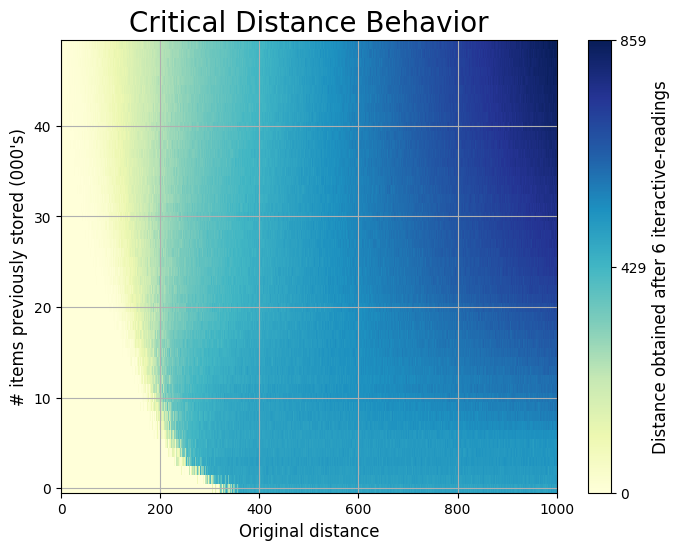
\includegraphics[width=3.1in]{./images02/new-images/kanerva-read.png}}

\subfloat[Chada's read]{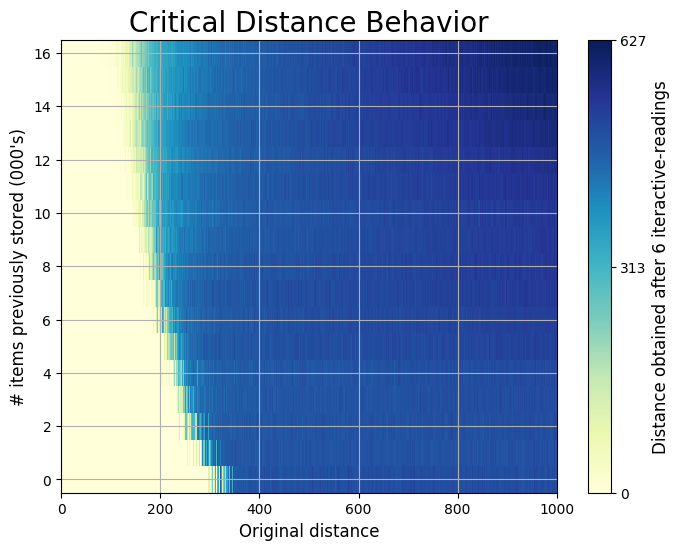
\includegraphics[width=3.1in]{./images02/new-images/chada-read_z_0.png}}
\caption{How far, in hamming distance, is a read item from the original stored item? Kanerva demonstrated that, after a small number of iterative readings (6 here), a critical distance behavior emerges. Items read at close distance converge rapidly; whereas farther items do not converge. Most striking is the point in which the system displays the tip-of-tongue behavior. Described by psychological moments when some features of the item are prominent in one's thoughts, yet the item still cannot be recalled (but an additional cue makes convergence `immediate'). Mathematically, this is the precise distance in which, despite having a relatively high number of cues (correct bits) about the desired item, the time to convergence is infinite.   Heatmap colors display the hamming distance the associative memory is able to cleanly converge to---or not.   In the $x$-axis, the distance from the desired item is displayed. In the $y$-axis, we display the read operation's behavior as the number of items registered in the memory grows.  These graphs are computing intensive, yet they can be easily tested by readers in our provided jupyter notebooks. Note the different scales.}
\label{fig:crit-dist-10k-writes}

\end{figure}

Figure \ref{fig:crit-dist-10k-writes} compares the critical distance behavior under different scenarios.  This replicates our previous results \citet{Brogliato2011} and \citet{brogliato2014sparse} and is a first part of the process of framework validation, to which we throw our attention next.



\chapter{Framework Architecture}

The framework implements the basic operations in a Sparse Distributed Memory which may be used to create more complex operations. It is developed in C language and the OpenCL parallel framework --- which may be loaded in many platforms and programming languages --- with a wrapper in Python. The Python module makes it easy to create and execute simulations in a Sparse Distributed Memory and works properly in Jupyter Notebook \citep{kluyver2016jupyter}. It works in both Python 2 and Python 3.

We split the SDM memory in two parts: the hard-location addresses and the hard-location counters. Thus, the addresses (bitstrings) of the hard-locations are stored in one array, while their counters in another. This makes possible to create multiple SDMs using the same address space, which would save computational effort to scan a bitstring in all the SDMs --- since they share the same address space, the activated hard-locations will be the same in all of them. As the slowest part of reading and writing operations is scanning the address space, the performance benefits are significant.

Each part may be stored either in the RAM memory or in a file. The RAM memory is interesting for quick experiments, automated tests, and others scenarios in which the SDM may be lost, while the file is interesting for a long-term SDM, like creating an SDM file with 10,000 random writes, which will be copied over and over to run multiple experiments. The file may also be sent to another researcher or may be published within the paper to let others run their own checks and verify the results. In summary, the framework fits many different uses and necessities.

Let a SDM memory with $N$ dimensions and $H$ hard-locations. Then, in a 64-bit computer, the array of hard-location addresses will use $H \cdot 8 \cdot \lceil N/64 \rceil$ bytes of memory, and there will be $H \cdot N$ hard-location counters. For example, in a SDM memory with 1,000 dimensions and 1,000,000 hard-locations, using 32-bit integers for the counters, the array of addresses will use 122MB of memory and the counters will use 3.8 GB of memory.

Basic operations were grouped in four sets: (i) for bitstrings, (ii) for addresses, (iii) for counters, and (iv) for memories (SDMs). Operations include creating new bitstrings, flipping bits, generating a bitstring with a specific distance from a given bitstring, scanning the address space using different algorithms, writing a bitstring to a counter, writing in an SDM, reading from an SDM, and iteratively reading from an SDM until convergence.


\section{Bitstring}

Bitstrings are the main structure of SDM. The addresses are represented in bitstrings, as well as the data. A bitstring is stored as an array of integers. Each integer may be 16-bit, 32-bit, or 64-bit long, depending on the configuration. By default, each integer is 64-bit long.

For instance, a 1,000-bit bitstring will have $\lceil 1000/64 \rceil = 16$ integers. These integers will have a total of $16 \cdot 64 = 1,024$ bits. The remaining 24 bits are always zero, so they do not affect the result of any operation. The memory usage efficiency is $1 - 24/1024 = 97.65\%$. Bitstrings store neither how many bits they have nor the array length. These pieces of information are only stored in the address space.


\subsection{The distance between two bitstrings}

The distance between two bitstrings is calculated by the hamming distance, which is the number of different bits between them. It is calculated counting the number of ones in the exclusive or (xor) between the bitstrings, i.e., $d(x, y) = \text{number of ones in } x \oplus y$.

There are several algorithms to calculate the number of ones \citep{warren2013hacker}, but the performance depends on the processor. So, we have implemented three different algorithms and one may be selected through compiling flags. The default algorithm is to use a built-in \_\_popcnt() instruction from the compiler.

There is also the naive algorithm, which really counts the number of ones checking bit by bit. It is available only to testing purposes and should never be used.

The other algorithm available is the lookup. It pre-calculates a table with the number of ones of all possible 16-bit integers. This table is accessed a few times to calculate the number of ones of a 64-bit integer, i.e., to calculate the distance between two bitstrings, it sums the distance of each 16-bit part of the bitstrings, i.e., $d(x[0:63], y[0:63]) = d(x[0:15], y[0:15]) + d(x[16:31], y[16:31]) + d(x[32:47], y[32:47]) + d(x[48:63], y[48:63])$ where $x[i:i+15]$ and $y[i, i+15]$ are the 16-bit integers formed by the bits between $i$ and $i+15$ of $x$ and $y$, respectivelly. Each 16-bit distance is calculated through a single table access. As each distance is calculated in O(1), this algorithm runs in O($\lceil bits/16 \rceil$). This table uses 65MB of RAM. One may change the table from 16-bit integers to 32-bit integers, which would halve the number of accesses at the expense of 4GB of RAM (instead of 65MB).


\section{Address space}

An address space is a fixed collection of bitstrings, and each bitstring represents a hard-location address. They store the number of bitstrings, as well as the number of bits, number of integers per bitstring, and the number of remaining bits.

Bitstrings are stored in a contiguous array of 64-bit integers, as shown in Figure \ref{tab:hl-addresses-detail}. Hence, basic pointer arithmetic provides us with performance improvements in their access, as processors realize fetches of contiguous chunks of memory  \citep{pai2004linux}.

\begin{figure}
\centering
\begin{tikzpicture}[
mycell/.style={draw, minimum size=7mm},
matrixA/.style={matrix of nodes,
    nodes={mycell, anchor=center},
    column sep=-\pgflinewidth,
    row sep=-\pgflinewidth,
    },
matrixB/.style={matrix of nodes,
    nodes={mycell, anchor=center},
    column sep=-\pgflinewidth,
    row sep=-\pgflinewidth,
}]

\matrix[matrixA] (A) { addr$_1$ & addr$_2$ & addr$_3$ & $\cdots$ & addr$_H$ \\ };

\matrix[matrixB, below=of A] (B) {
addr$_{k, 1}$ & addr$_{k, 2}$ & addr$_{k, 3}$ & $\cdots$ & addr$_{k, 8 \cdot \lceil N/64 \rceil}$ \\
};

\draw[dashed] (A-1-1.south west)--(B-1-1.north west);
\draw[dashed] (A-1-1.south east)--(B-1-5.north east);
\draw [
	thick,
    decoration={
        brace,
        mirror,
		amplitude=0.2cm,
        raise=0.2cm
    },
    decorate
] (B-1-1.south west) -- (B-1-5.south east)
node [pos=0.5,anchor=north,yshift=-0.5cm] {N bits};

\end{tikzpicture}

\caption{Address space's bitstrings are stored in a contiguous array. In a 64-bit computer, each bitstring is stored in a sub-array of 64-bit integers, with length $8 \cdot \lceil N/64 \rceil$.\label{tab:hl-addresses-detail}}
\end{figure}

The scan for activated hard-locations is performed in an address space. It returns the indexes of the bitstrings which were inside the circle (and their distances). Then, each operation uses these pieces of information in a different way.

\subsection{Scanning for activated hard-locations}

Scanning for the activated hard-locations is a problem similar to well-known problems in computational geometry called ``range reporting in higher dimensions''. In this case, none of the known algorithms is able to solve our problem faster than $O(H)$. The algorithm which seems to best fit in our problem consumes $O(H)$ space and runs in $O(\log^n(H))$ \citep{chazelle1988functional}, which is really slower than $O(H)$ when, for instance, $H=1,000,000$ and $n=1,000$. For a review of the range reporting algorithms, see \citet{chan2011orthogonal}.

In 2014, there was published a solution to fast search in hamming space which seems applicable to our problem \citet{norouzi2014fast}. It provides a fast search when $r/n < 0.11$ or $r/n < 0.06$, where $r$ is the radius and $n$ is the number of bits. But, in our case, for a 1,000 bits SDM, $r/n = 0.451$, which changes the runtime to $O(H^{0.993})$. This is really close to $O(H)$, but with a larger constant. Unfortunately, $O(H)$ is still faster.

It is intriguing that none of those algorithms is able to solve our scanning problem. The idea behind those computational geometry algorithms is roughly to split the search space in half each step, which would take $O(\log(H))$ to go through the whole space. But this approach does not work because of the high number of dimensions (i.e., 1,000) and because the hard-locations' addresses are randomly sampled from the $\{0, 1\}^n$ space. Although each addresses' bit itself splits the hardlocations in half, it does not split the search space in half since both halves still must be convered by the algorithm. For instance, let's say we have $n=1,000$ dimensions with $H=1,000,000$ hard-locations, and we are scanning within a circle with radius $r=451$, then after checking the first bit we have two cases: (i) for the half with the same first bit, we must keep scanning with radius 451; and (ii) for the half with a different first bit, we must keep scanning with radius 450. Hence, the search space has not been split in half because both halves have been covered (and one of them should have been skipped).

Finally, as our best approach is to scan through all hard-locations, we may distribute the scan into many tasks which will be executed independently. The tasks may be executed in different processes, threads, or even computers. They may also run in the CPU or in the GPU. In this case, we may take into account both the time required to distribute the tasks and the time to receive their results.

The framework implements three main scanner algorithms: linear scanner, thread scanner, and OpenCL scanner. The linear scanner runs in a single core, is the slowest one, and was developed only for testing purposes; the thread scanner runs at the CPU in multiple threads sharing memory (and our recommendation is to use the number of threads equals to twice the number of CPU cores); and the OpenCL scanner runs in multiple GPU cores and support multiple devices. The speed of a scan depends on the CPU and GPU devices, thus the best approach to choose which scanner is best for one's setup is to run a benchmark.

The OpenCL must be initialized, which just copies the address space's bitstrings to the GPU's memory. Then, many scans may be executed with no necessity to upload the bitstrings again. The OpenCL scanner supports running into multiple devices.


\section{Counters}

Each hard-location has one integer of data per bit. For instance, each hard-location of a 1,000 bits SDM has 1,000 bits. Those integers are stored in a counter.

A counter is an array of integers which stores the data of all hard-locations. So, the counter's array has $n \cdot H$ integers.

When two counters are added in a third counter, there may occur an overflow. It is not supposed to be a problem because, by default, each counter is a signed 32-bit integer that can store any number between -2,147,483,648 and 2,147,483,647, which means they will not overflow with less writes than $2^{31}-1$ divided by the average number of activated hard-locations. For instance, when $n=1,000$, $H=1,000,000$, and $r=451$, the average number of activated hard-locations is 1,000 and it would require at least one million writes before being possible to a counter to overflow.  Note also that it would be more likely to saturate the memory before any overflow.

Anyway, counters may have overflow protection depending on compiling options. By default, there is no overflow check for performance reasons (and because it does not seem necessary).

\section{Read and write operations}

The reading and writing operations are executed in two steps: first, the address space is swept looking for the activated addresses; then, the operation is performed in the counters. Reading operation assemblies the bitstring according to the counters of the activated addresses, while the writing operation changes the counters.

The iterated reading keeps reading until it gets exactly the same bitstring (or the number of maximum interations has been reached), i.e., it performs $\eta_{i+1} = \text{read}(\eta_i)$ and stops when $\eta_{k+1} = \eta_{k}$. If the initial bitstring is inside the critical distance of $\eta$, it will converge to $\eta$, but, if it is not, it will diverge and reach the maximum number of iterations.

The framework has both Kanerva's read and the generalized read. The latter was implemented according to the generalization proposed by professor Paulo Murilo. The generalization brings a parameter $z$, which is the exponent. In this case, the results are floating point instead of integer, which considerably reduces performance. When $z=1$, it is exactly as the Kanerva's read. When $z=0$, it is the Chada's read. We also explored how SDM would behave for different values of $z$.

There is another special read operation: the weighted reading. In the weighted reading, the value of the counters are multiplied by a weight which depends only on the distance between the reading address and the hard-location address. The weight is retrieved from a lookup table of integers indexed by the distance. The rest of the read operation is exactly the same.

There is also a weighted writing operation. In this case, the weight is applied when the counters are updated, i.e., if the weight is 2, the counters are increased twice when bits are 1, and decreased twice when bits are 0. Just as in the weighted reading, the weights depend only on the distance between the writing address and the hard-location address. The weights are retrieved from a lookup table of integers indexed by the distance.


\chapter{Results (i): Framework Validation}

The framework has been validated comparing its results with the expected results from \citet{Kanerva1988}. Thus, we run simulations which were then compared to the theoretical analysis conducted some decades ago.

The objective here is twofold: (i) a single command will install the framework, and (ii) another single command will run (and display) the desired figures obtained the simulation. This will allow potential users to become familiarized with the system and its underlying code with barely any learning curve beyond scientific python and jupyter notebooks.

One particular analysis of interest is that of the distance read at a point $\alpha$. Suppose an SDM is trying to read an item written at $\alpha$, but the cues received so far lead to a point of distance $d$ from $\alpha$.  As one reads at $\alpha+d$, a new bitstring $\beta$ is obtained, leading to our question: what is the new distance from $\alpha$ to $\beta$? Is it smaller or larger than $d$? That, of course, depends on the ratio between $d$ and the number of dimensions of the memory.  As we have found out, there are some deviations from Kanerva's original theoretical analysis and the results obtained by simulation.

\subsection{Some initial anomalous results}

As we ran the simulations reflecting some of Kanerva's graphs, one in particular struck our attention: The new distances obtained after a read operation were not perfectly predicted by the theoretical model, and we propose that this is due to interaction effects between different attractors.

\citet{Kanerva1988} originally predicted a \textasciitilde 500-bit distance after a point (Fig. \ref{kanerva-table-7-2}). The original prediction considered that the read distance would decline when inside the critical distance in increase afterwards, converging to a \textasciitilde 500-bit distance.  At this point, each read would lead to a different, orthogonal, \textasciitilde 500-bit distance point.

\begin{figure}[h]
\centering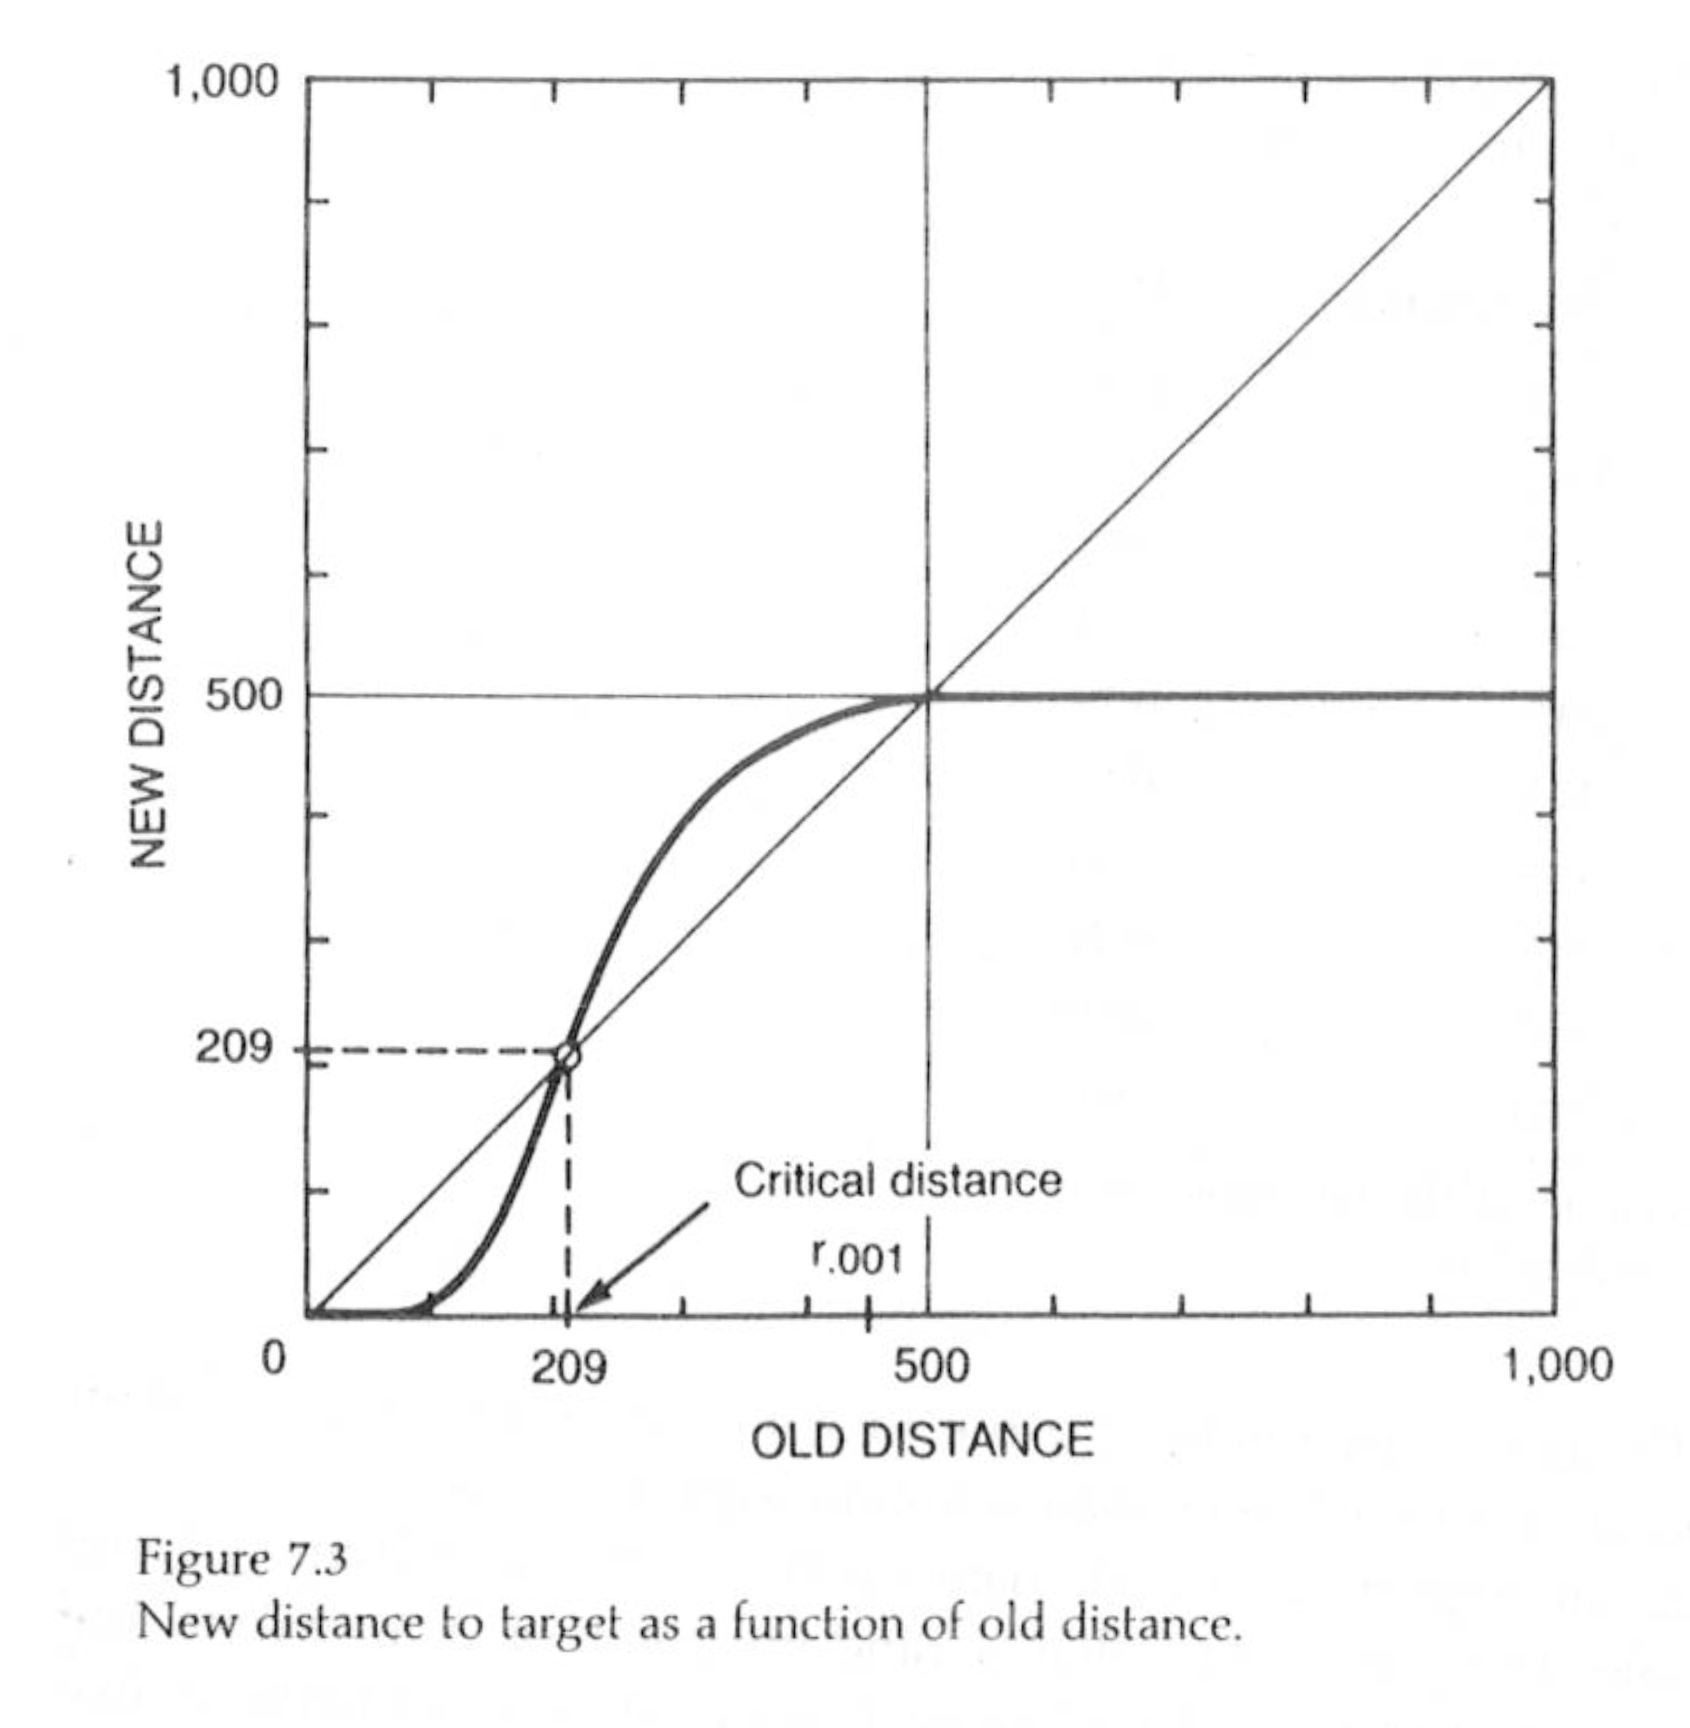
\includegraphics[width=0.8\textwidth]{images02/kanerva-table-7-2-original.png}
\caption{Kanerva's original Figure 7.3 (p. 70) predicting a \textasciitilde 500-bit distance after a point.
\label{kanerva-table-7-2}}
\end{figure}

Our preliminary results show that the theoretical prediction is not accurate.  There are interaction effects from one or more of the attractors created by the 10,000 writes, and these attractors seem to raise the distance beyond \textasciitilde 500 bits (Fig. \ref{sdm-10000w-table-7-2}). Our results were obtained using a 1,000 bit, 1,000,000 hard-location SDM with exactly 10,000 random bitstrings written into it, the same used by Kanerva.

\begin{figure}[h]
\centering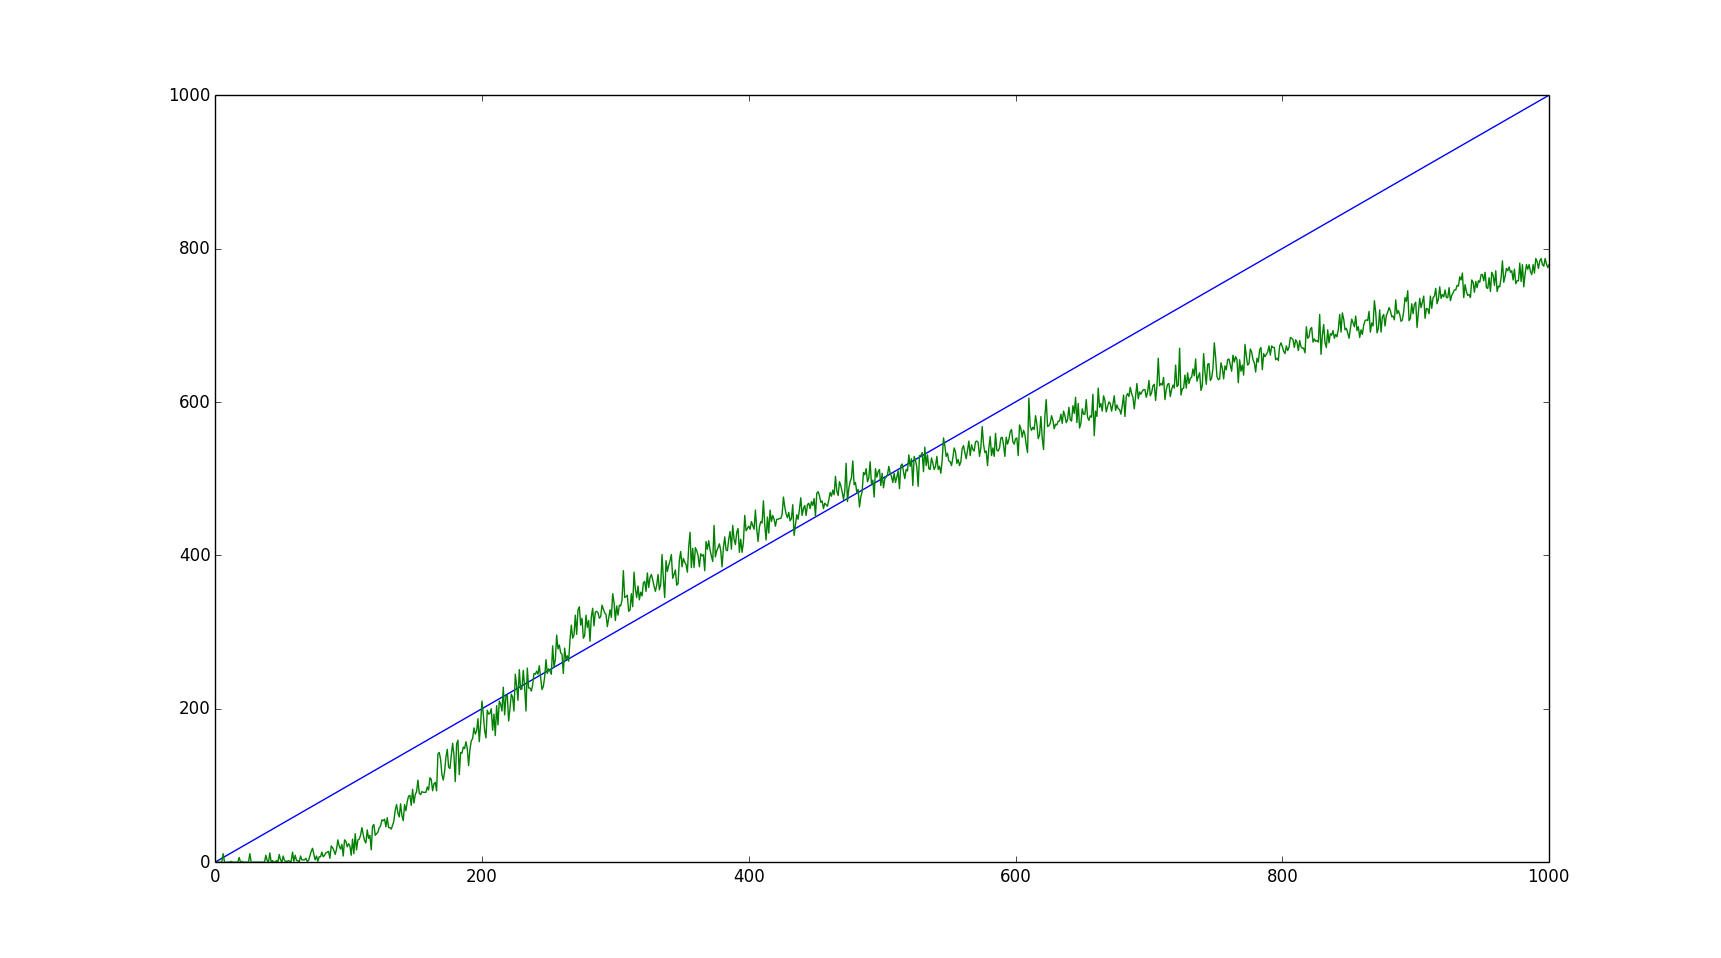
\includegraphics[width=0.8\textwidth]{images02/sdm-10000w-table-7-2.png}
\caption{Results generated by the framework diverging from Kanerva's original Table 7.2. Here we had a 1,000 bit, 1,000,000 hard-location SDM with exactly 10,000 random bitstrings written into it, which was also Kanerva's configuration.
\label{sdm-10000w-table-7-2}}
\end{figure}

But, when we reduced the number of random bitstrings written in the SDM from 10,000 to only 100, the results reflected very well the Kanerva's theoretical expectation (Fig. \ref{sdm-100w-table-7-2}). This result strengthens our hypothesis that the disparities in the computational results are due to the interaction effect of high numbers of different attractors.

\begin{figure}[h]
\centering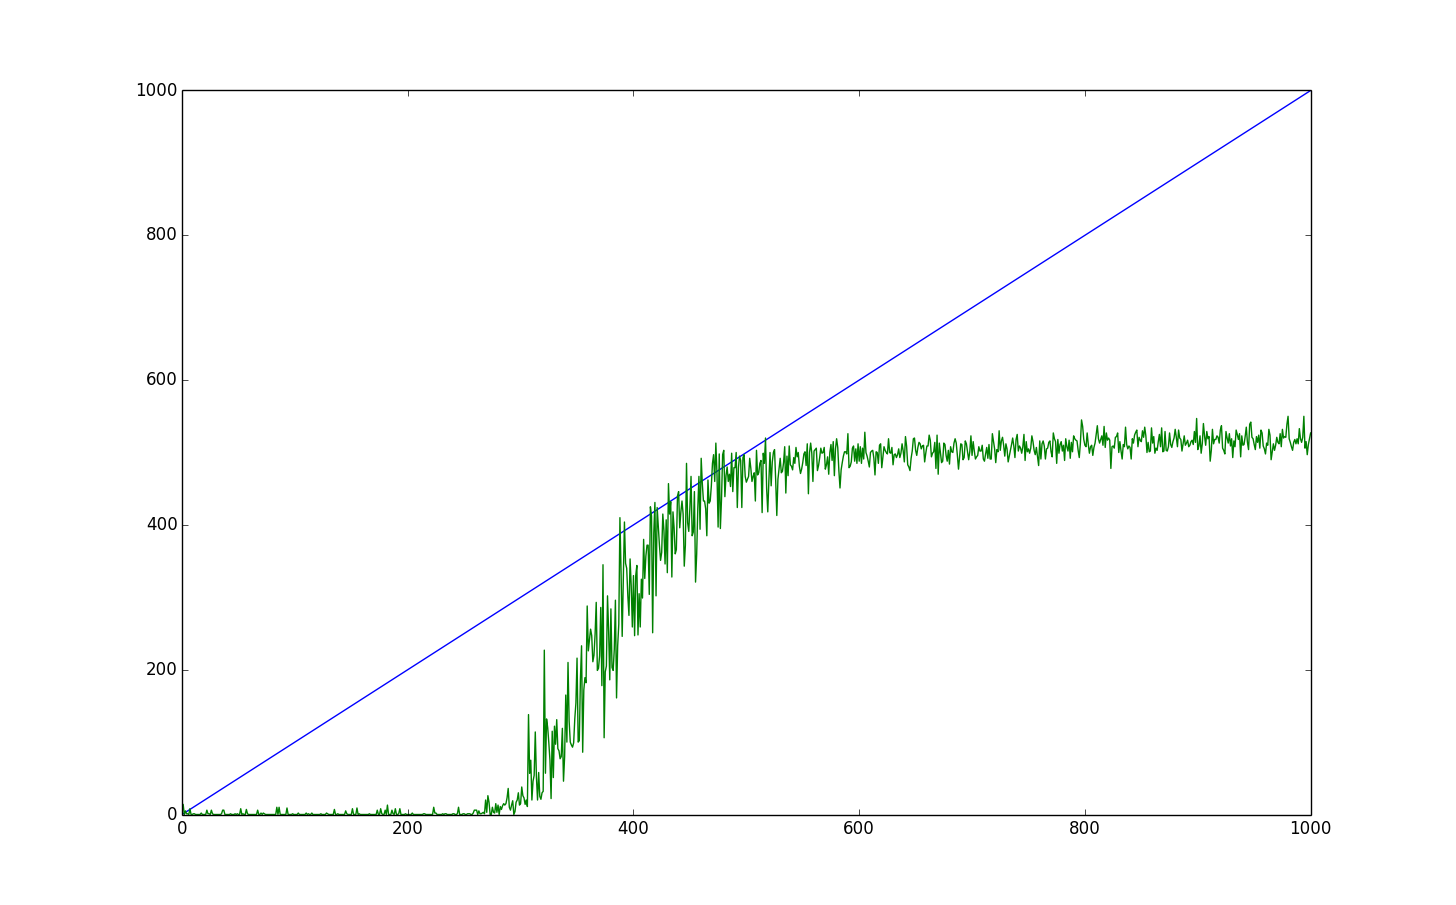
\includegraphics[width=0.8\textwidth]{images02/sdm-100w-table-7-2.png}
\caption{Results generated by the framework similar from Kanerva's original Table 7.2. It was a 1,000 bit, 1,000,000 hard-location SDM with exactly 100 random bitstrings written into it.
\label{sdm-100w-table-7-2}}
\end{figure}

To obtain the results from Fig. \ref{sdm-10000w-table-7-2} and \ref{sdm-100w-table-7-2}, we had to write 10,000 random bitstrings to an SDM, and then randomly choose one of those bitstrings to be our origin. Finally, we randomly flipped some bits from the origin bitstring and executed a reading operation in the SDM. Thereby, in order to show the interaction effects more clearly, we wrote a handmade bitstring to the SDM which had all bits inverted in relation to the origin bitstring --- their hamming distance was equal to 1,000. Our handmade bitstring was acting as an opposite attractor, and one can see the accelerating effects towards convergence to both attractors: the origin and the handmade bitstrings (Fig. \ref{sdm-10000w-notX-table-7-2}). Here we had the exact same configuration of Figure \ref{sdm-10000w-table-7-2}, with the addition of the single opposite attractor.

\begin{figure}[h]
\centering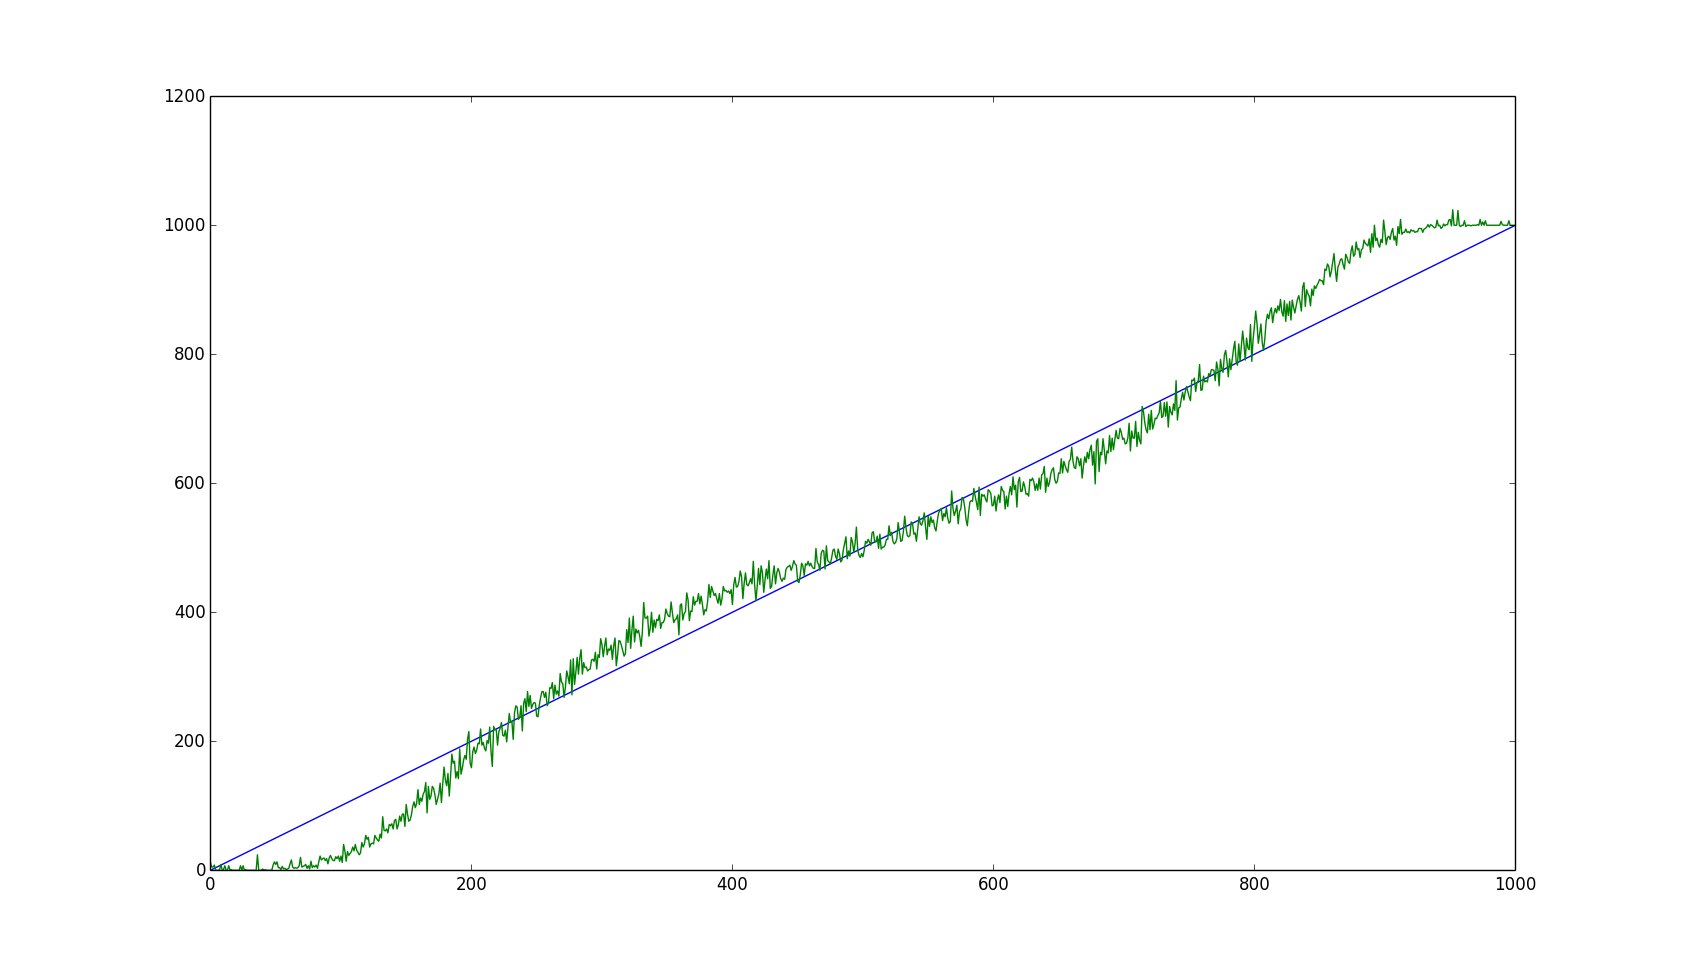
\includegraphics[width=0.8\textwidth]{images02/sdm-10000w-notX-table-7-2.png}
\caption{This graph shows the interaction effects more clearly.  As we include an opposite bitstring, one can see the accelerating effects towards convergence to both attractors: the origin and the opposite. Here we have the exact same configuration of Figure \ref{sdm-10000w-table-7-2}, with the addition of the single opposite attractor.
\label{sdm-10000w-notX-table-7-2}}
\end{figure}

Obviously, these small deviations from Kanerva's original theoretical predictions deserve a qualification.  Kanerva was working in the 1980s and the 1990s, and had no access to the immense computational power that we do today. It is no surprise that some small interaction effects should exist as machines allow us to explore the ideas of his monumental work.

\begin{figure}[h!]
  \centering
  \subfloat[$z \in \{.1, .2, .3, .4, .5, 1\}$]{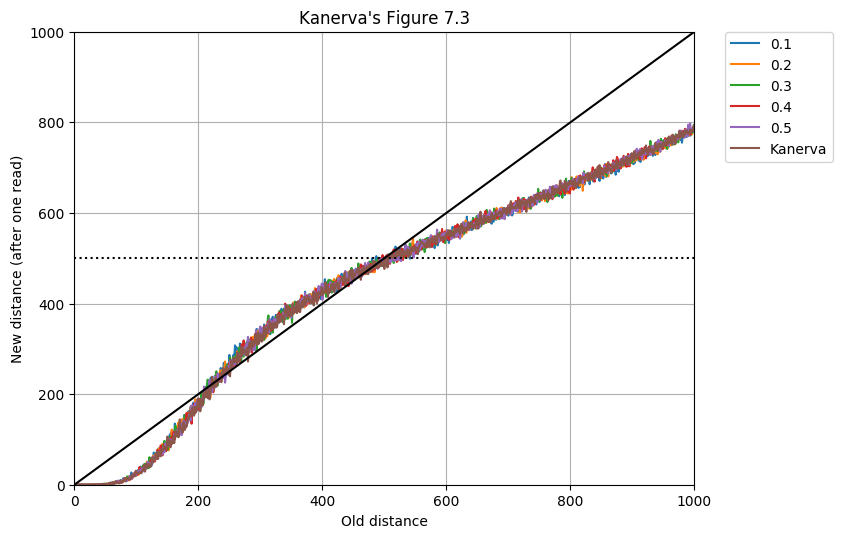
\includegraphics[width=2.9in]{./images02/new-images/iter_z_01-05.png}}
  \subfloat[$z \in \{1.5, 3, 4.5, 6\}$]{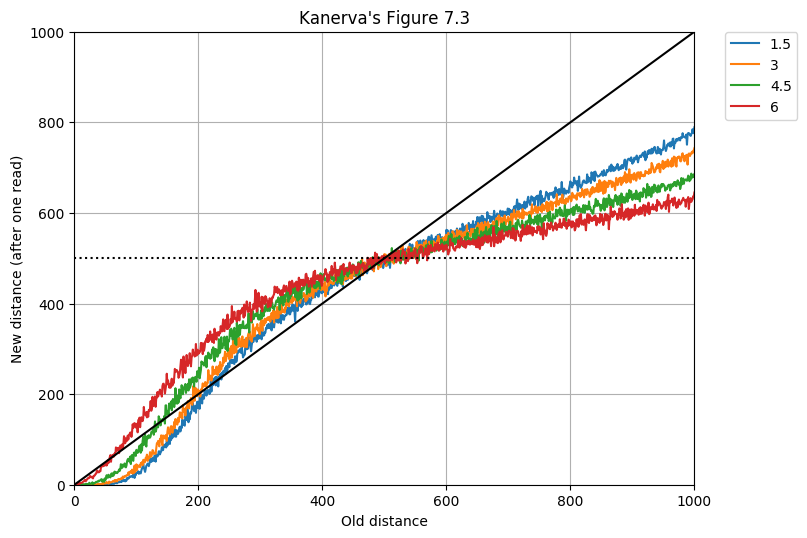
\includegraphics[width=2.9in]{./images02/new-images/z_15_3_45_6.png}}

  \subfloat[$z \in \{0, 1\}$]{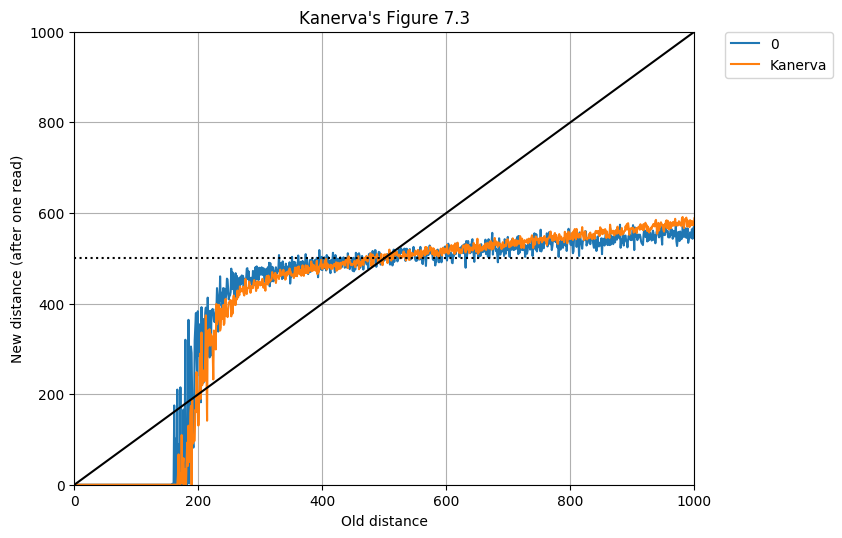
\includegraphics[width=2.9in]{./images02/new-images/z_0_1.png}}
  \subfloat[$z \in \{0, 0.5, 1, 1.5, 3, 4.5, 6\}$]{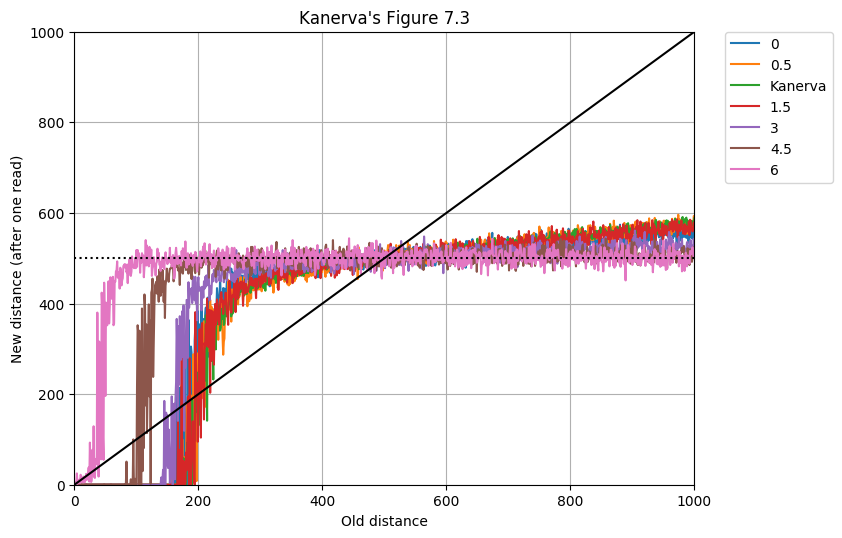
\includegraphics[width=2.9in]{./images02/new-images/iter_z_all_2.png}}

  \caption{(a) and (b) show the behavior of a single read; (c) and (d) present the effects of 6 iterative reads. As stated previously, we can see a deterioration of convergence, with lower critical distance as $z>1$.  Another observation can be made here, concerning the discrepancy of Kanerva's Fig 7.3 and our data.  It seems that Kanerva may not have considered that a single read would only `clean' a small number of dimensions \emph{after the critical distance}. What we observe clearly is that with a single read, as the distance grows, the system only `cleans' towards the orthoghonal distance 500 after a number of iterative readings.}
  \label{fig:murillo-generalization-experiments}
\end{figure}

Physicist Paulo Murilo observed that the models of Kanerva-read ($z=1$) and Chada-read ($z=0$) were simple variations of the exponent $z$, which suggests experimenting with different values. The results, however, have not yielded performance improvements.  Though for $z \leq 1$ results are comparable to $z=1$, for $z>1$, the system shows a clear deterioration, with a smaller distance to convergence and higher divergence at large-distance reads. This is shown in Figure \ref{fig:murillo-generalization-experiments}.



\chapter{Results (ii): Performance}

Our intention is to provide comparative performance metrics under different computation engines (CPU, GPU, etc) and different operating systems (Linux, MacOs, Windows, etc). Performance can be measured as the average number of scans of all hard locations per second, reads per second, writes per second, etc.

Our first device is a personal MacBook Pro Retina 13-inch Late 2013 with a 2.6GHz Intel core i5 processor, 6GB DDR3 RAM, and Intel Iris GPU.  We also intend to test on machines such as the iMac with dedicated GPU, MacPro with dedicated GPU, and personal computers under Linux with dedicated GPUs.

Beyond that, we are running as state-of-the-art devices: (i) an Amazon EC2 p3.xlarge with Intel Xeon E5-2686v4 processor, 61GB DDR3 RAM, and NVIDIA K80 GPU, and (ii) an Amazon EC2 p3.8xlarge with Intel Xeon E5-2686v4 processor, 488GB DDR3 RAM, and 8x NVIDIA K80 GPU.

% !TEX root = ../partial-sdm.tex

\section{Results (iv): Supervised classification application}

Supervised classification problem consists of categorize data into groups after seeing some samples from each group. First, it is presented pieces of data with their categories. The algorithm learns from these data, which is known as learning phase. Then, new pieces of data are presented and the algorithm must classify them into the already known groups. It is named supervised because  the algorithm will not create the groups itself. It will learn the groups from during the learning phase, in which the groups have already been defined and the pieces of data have already been classified into them.

Although this problem has already been studied (REF), our intention here is to show that a pure SDM may also be used to classify data. \citet{fan1997genetic} has used SDM to solve a classification problem, recognizing handwriting letters from images, but he used a mix of genetic algorithm with SDM, which is very different from the original SDM described by \cite{Kanerva1988}. Even though his algorithm has classified properly, we were intrigued whether a pure SDM would also classify successfully.

Hence, we have developed a supervised classification algorithm based on a pure SDM as our main memory. Our goal was to classify noisy images into their respective letters (case sensitive) and numbers. For some examples, see Figure \ref{fig-classification-examples}.

\begin{figure}[!htb]
\centering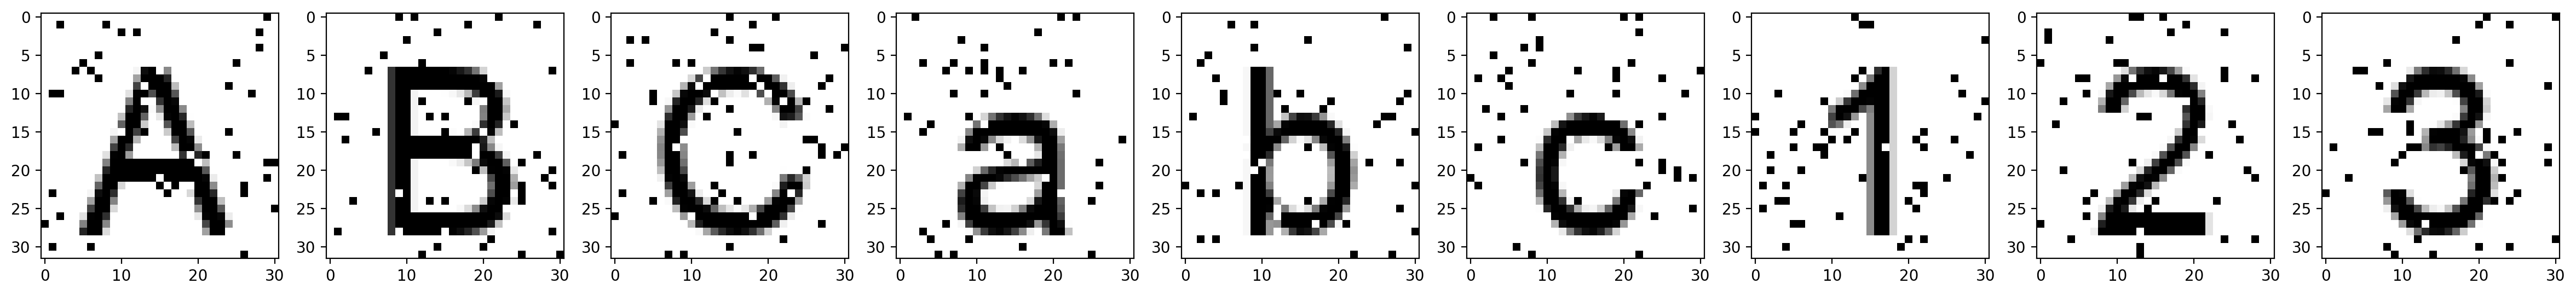
\includegraphics[width=\textwidth]{./images02/classification/example.png}
\caption{Examples of noisy images with uppercase letters, lowercase letters and numbers.
\label{fig-classification-examples}}
\end{figure}

The images had 31 pixels of width and 32 pixels of height, totaling 992 pixels per image. Each image was mapped into a 1,000 bit bitstring in which the bits were set according to the color of each pixel of the image. So, white pixels were equal to bit 0, and black pixels to bit 1. The 8 remaining bits were all set to zero. This was a bijective mapping (or one-to-one mapping), i.e., there was only one bitstring for each image, and there was only one image for each bitstring.

% TODO Add image showing the association between pixels and bits.

A total of 62 classification groups have been trained in the SDM. For each of them, it was generated a random bitstring. Thus, the groups' bitstrings were orthogonal between any two of them. There is one image for each of the 62 groups in Figure \ref{fig-classification-groups}. Notice that the SDM has never seen a single image with no noise.

\begin{figure}[!htb]
\centering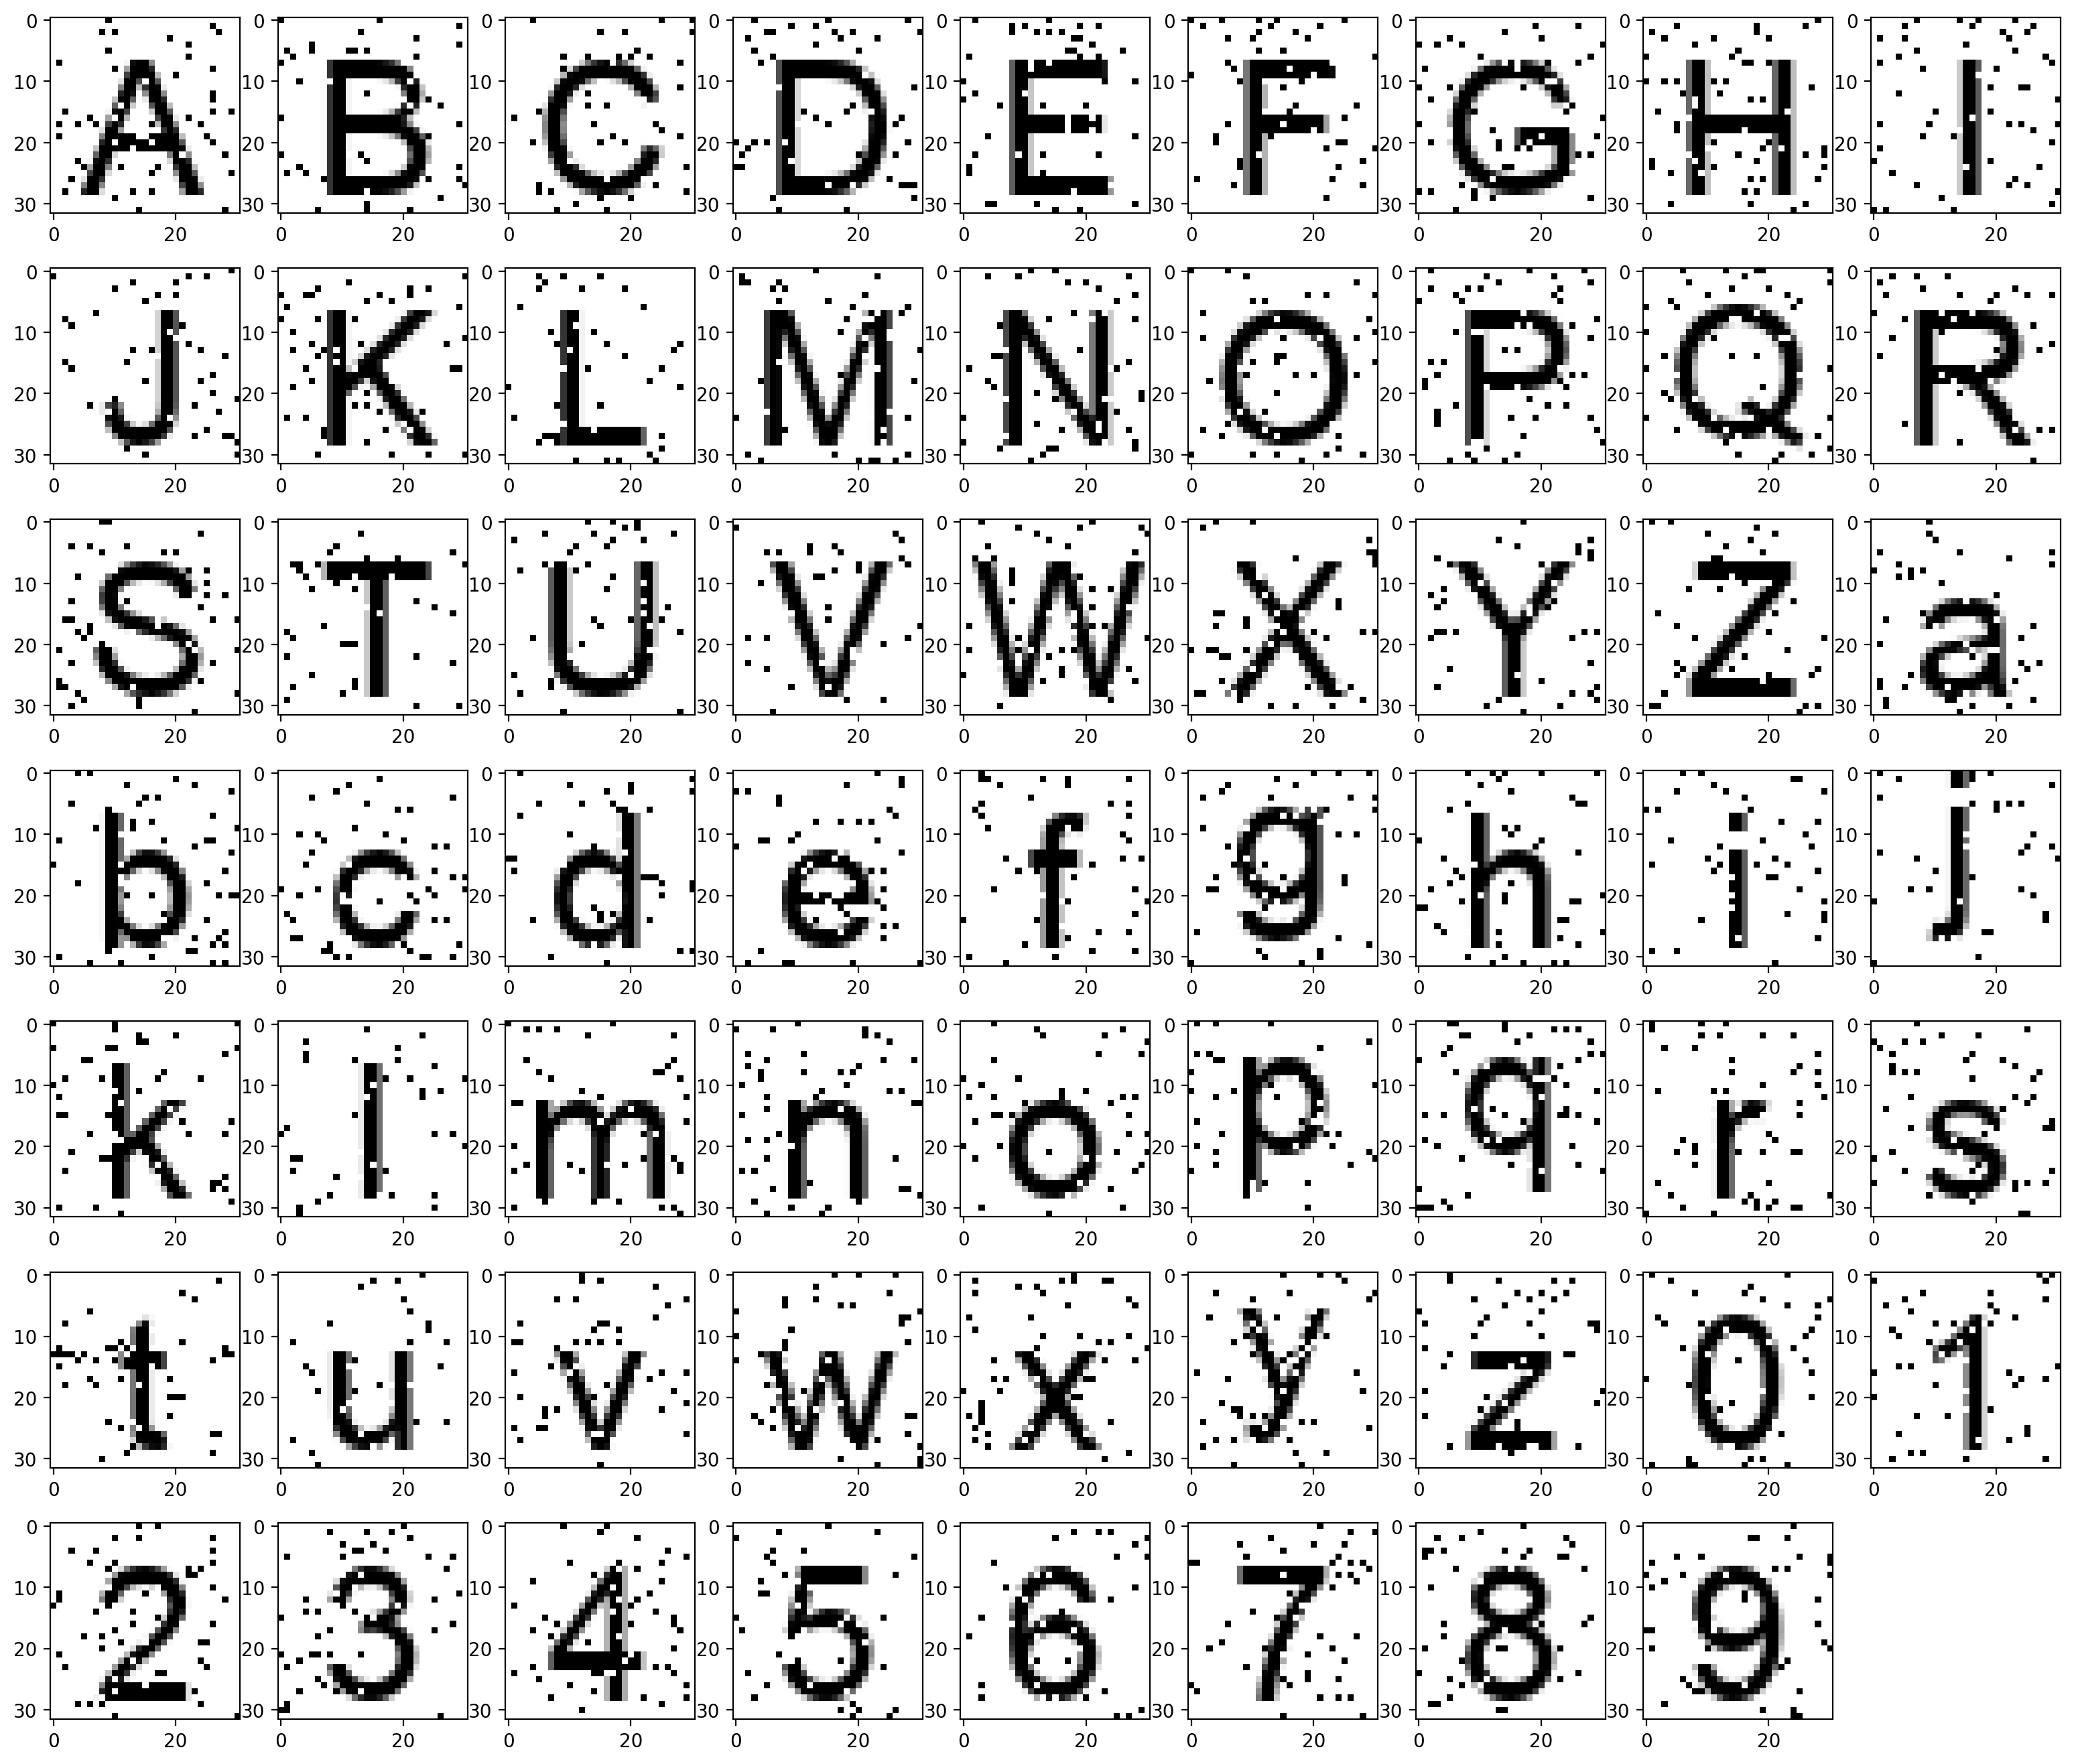
\includegraphics[width=\textwidth]{./images02/classification/groups.png}
\caption{One noisy image for each of the 62 classification groups.
\label{fig-classification-groups}}
\end{figure}

The association of images to groups was stored as sequences in SDM, as detailed by \citet{Kanerva1988} in Chapter 8. During the learning phase, the image bitstrings were stored pointing to their groups bitstrings, i.e., write(addr=bs\_image, datum=bs\_label). Thus, in order to classify an unknown image, we only had to read from its address and check which group has been found.

% TODO Add image showing the pointers.

During the learning phase, we have generated 100 noisy images for each character. The images had 5\% of noise, i.e., 5\% of their pixels have been randomly flipped. For example, see the generated images for letter A in Figure \ref{fig-classification-training-A}. Then, we have wrote the classification group bitstring into the bitstring associated to each noisy image, i.e., write(bs\_image, bs\_label). For a complete image training set, see Appendix XYZ.

\begin{figure}[!htb]
\centering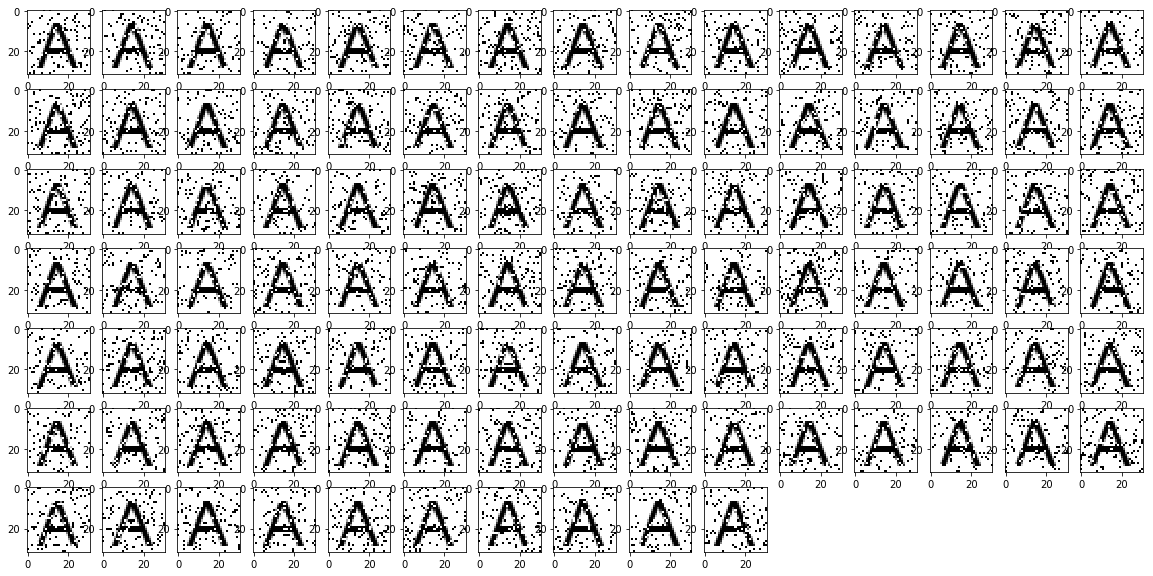
\includegraphics[width=\textwidth]{./images02/classification/trainingA.png}
\caption{100 noisy images generated to train label A.
\label{fig-classification-training-A}}
\end{figure}

Finally, we have assess the performance of our classifier. We had done it in three different scenarios: high noise (20\%), low noise (5\%) and no noise. See Figures \ref{fig-classification-noise-high} and \ref{fig-classification-no-noise} for images with 20\% noise and no noise. The low noise scenario had the same noise as the training set. For each scenario, we had classified 620 unknown images with 10 images per group.

\begin{figure}[!htb]
\centering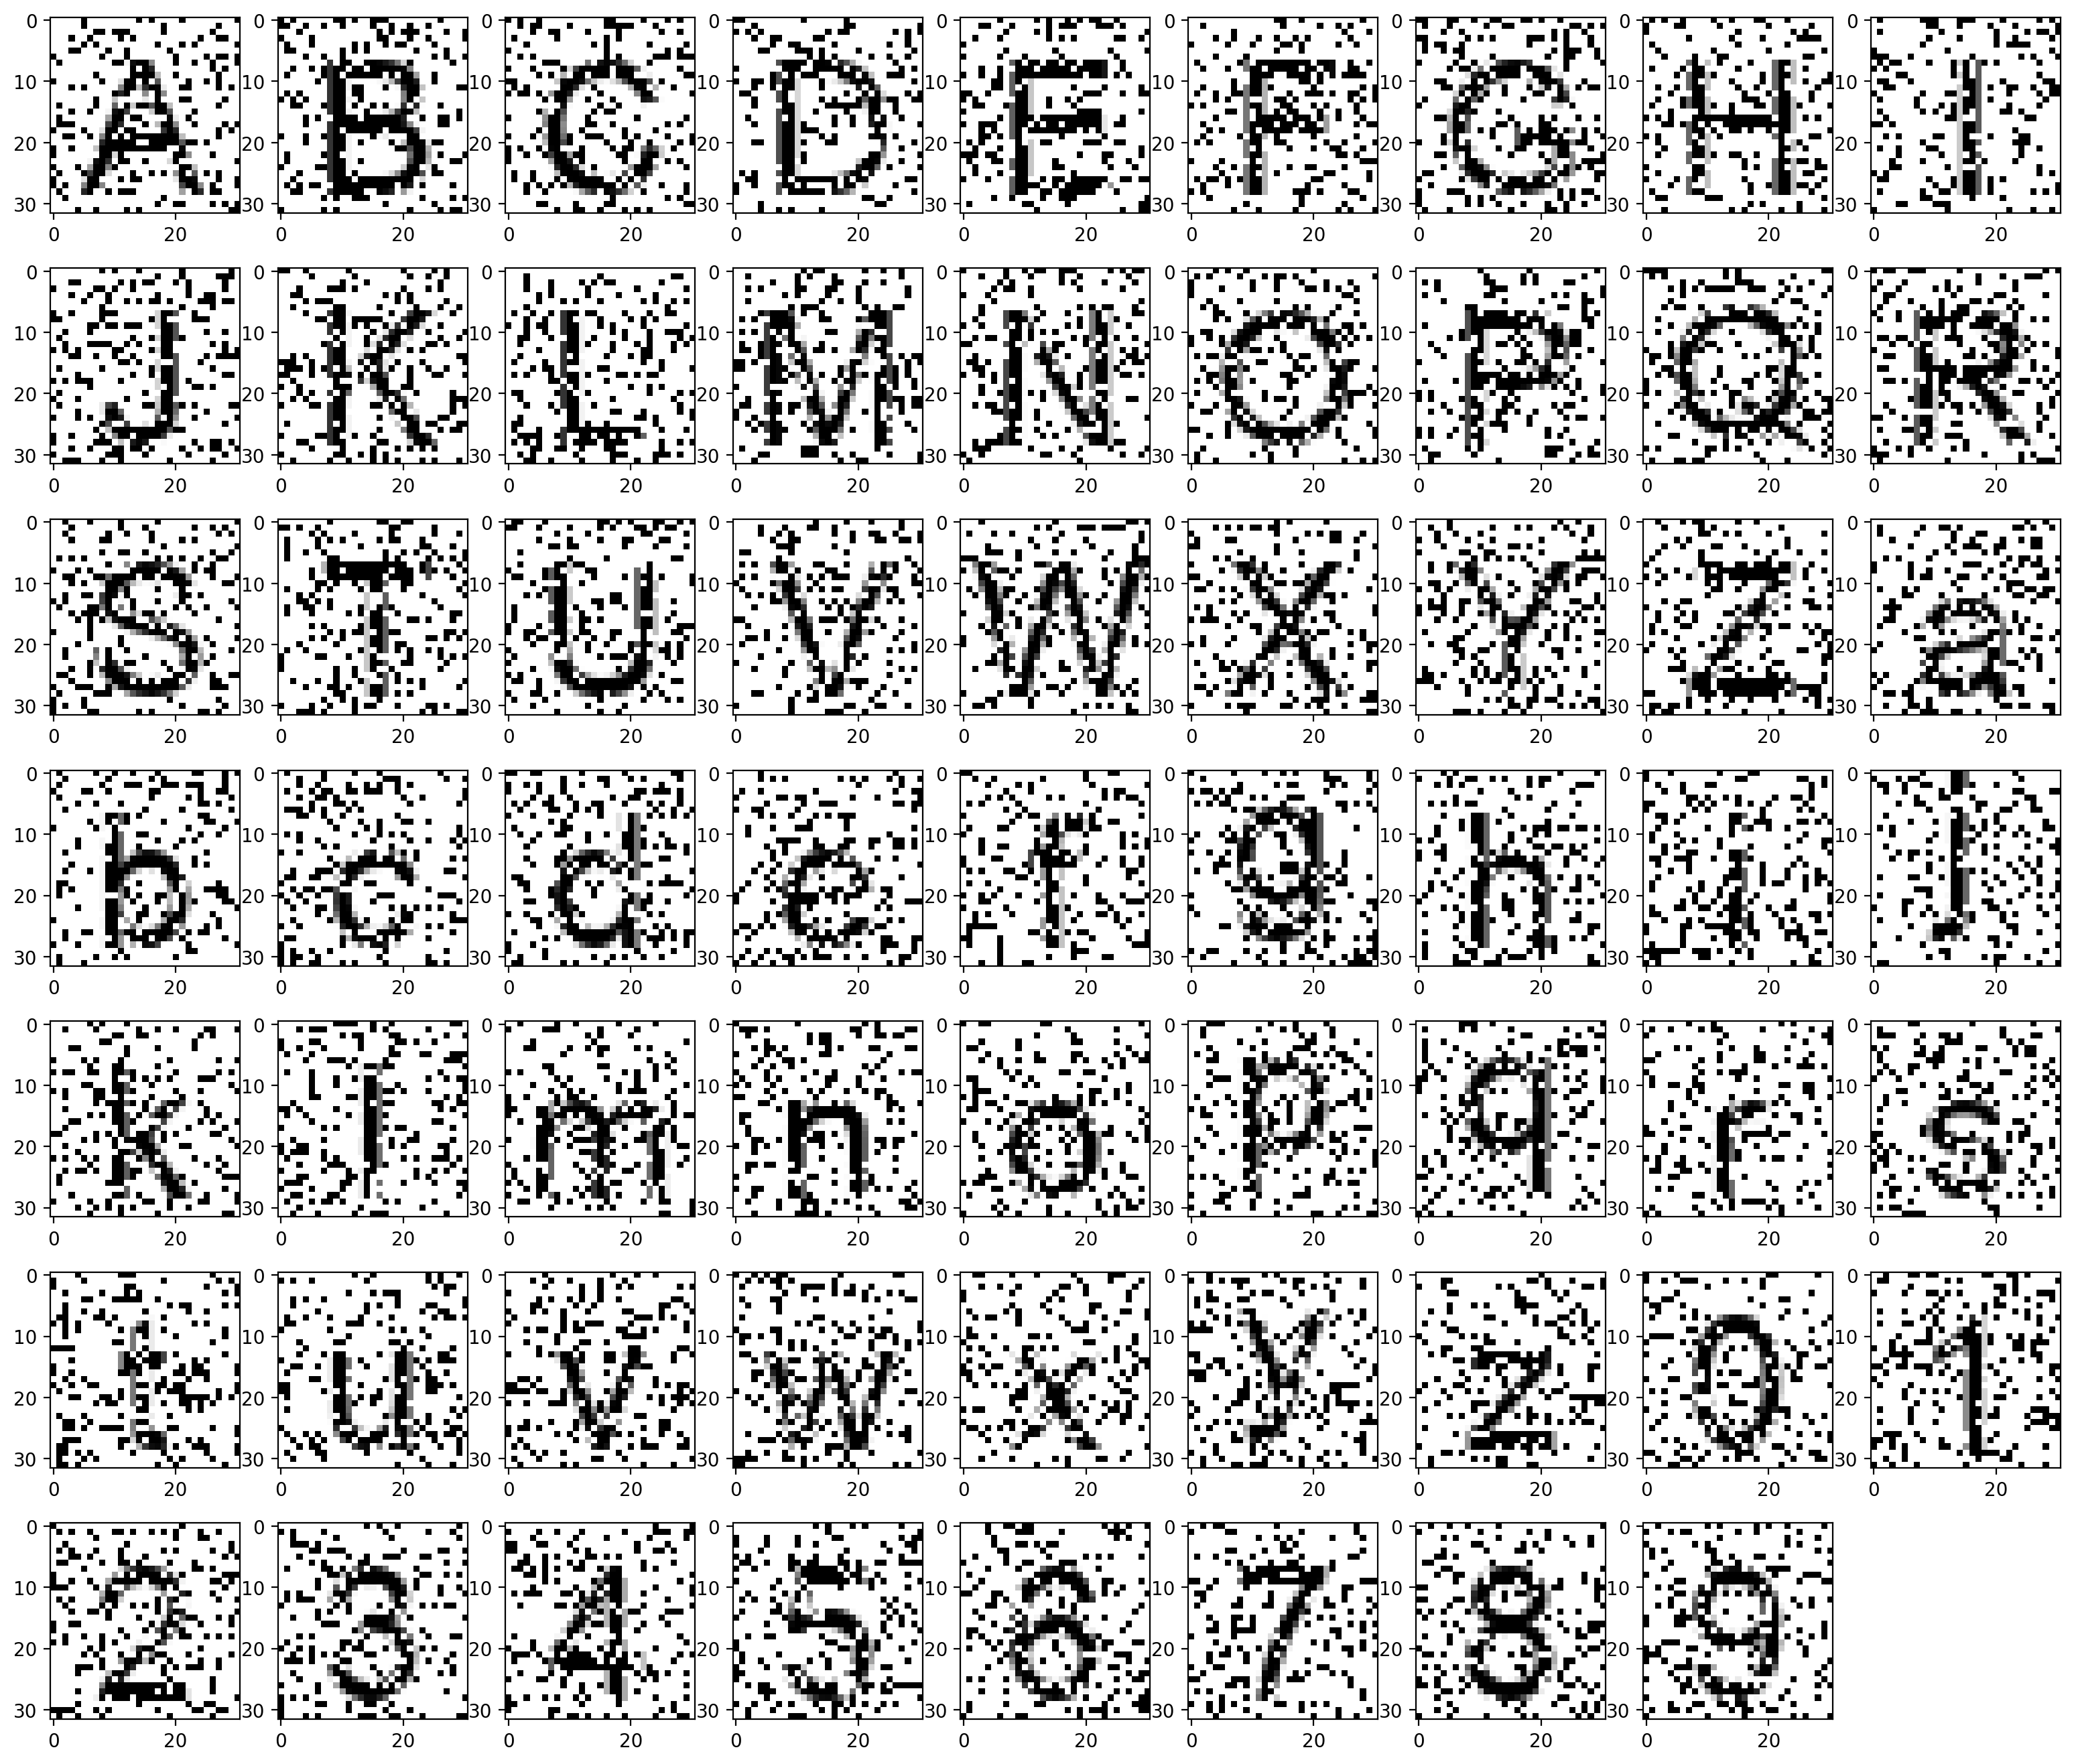
\includegraphics[width=0.75\textwidth]{./images02/classification/noise-high.png}
\caption{Images generated using a 20\% noise for the high noise scenario.
\label{fig-classification-noise-high}}
\end{figure}

\begin{figure}[!htb]
\centering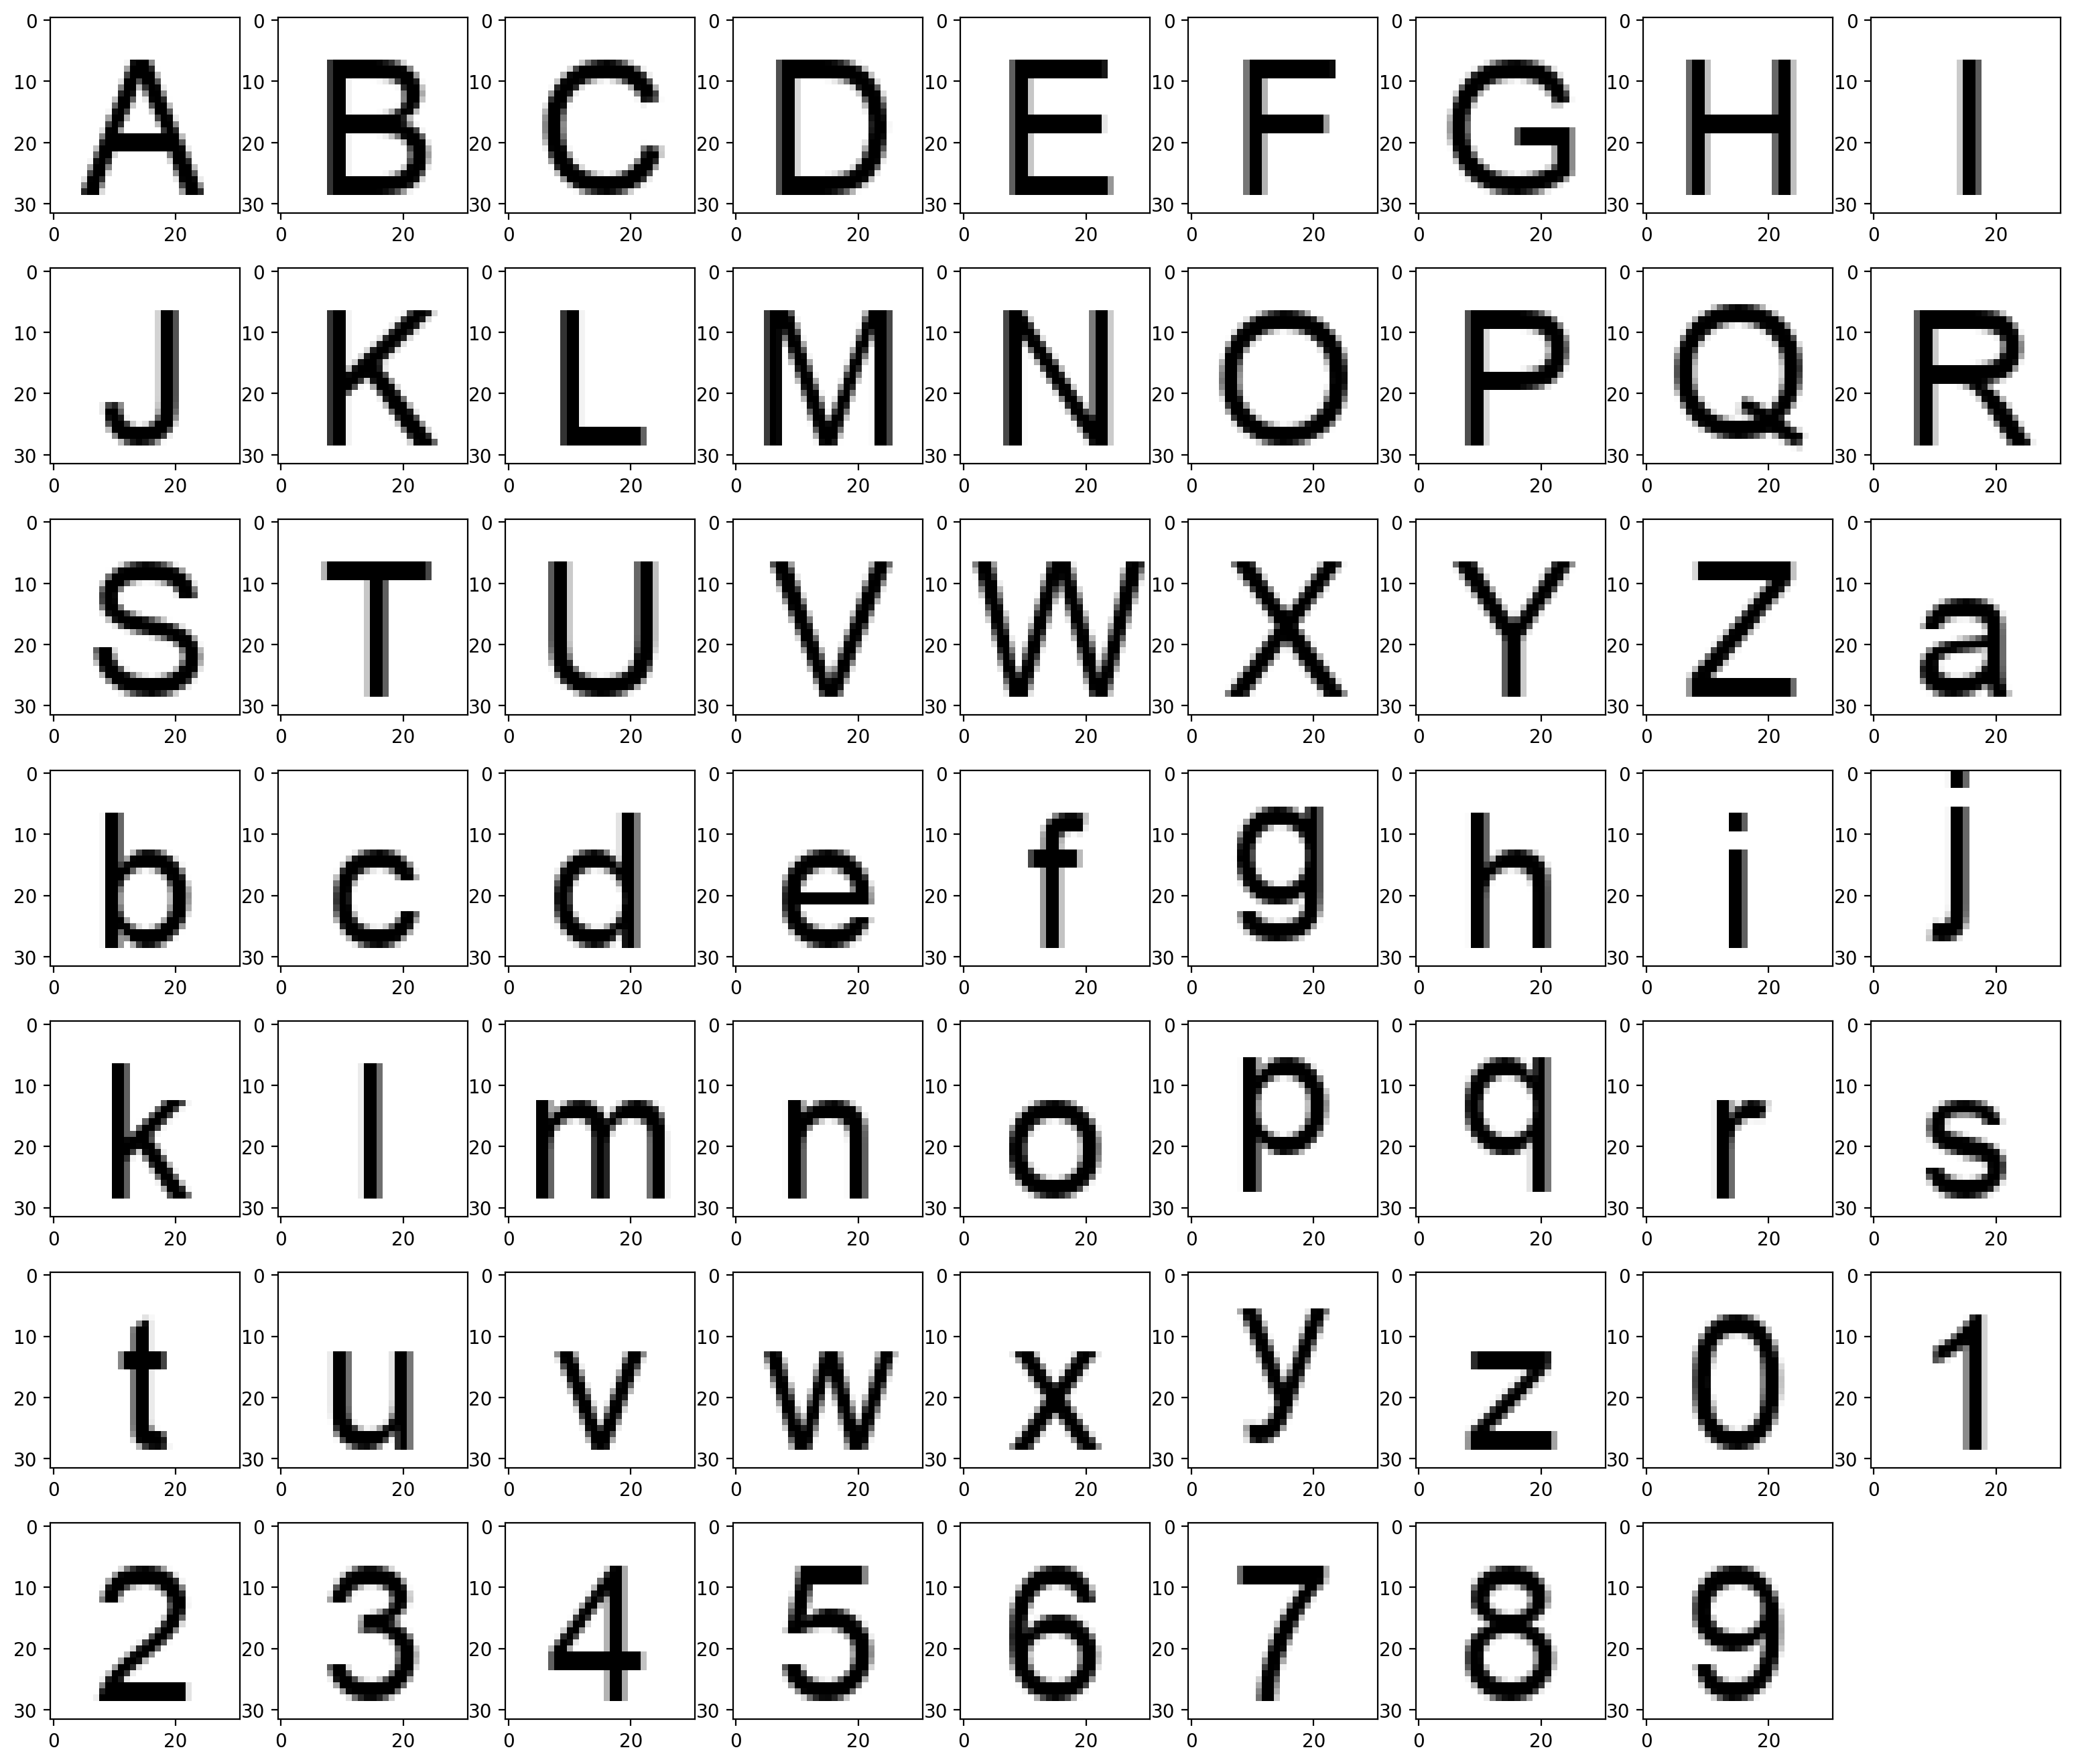
\includegraphics[width=0.75\textwidth]{./images02/classification/no-noise.png}
\caption{Images generated for the no noise scenario.
\label{fig-classification-no-noise}}
\end{figure}

The performance was calculated as the percentage of hits for each group. We did not expected the same performance for all groups because some groups become very similar to other depending on the noise level, and this similarity may even confuse a person (see Figure \ref{fig-classification-similarity}).

\begin{figure}[!htb]
  \centering
  \subfloat[``i'', ``l'', and ``r'' with 20\% noise.]{\includegraphics[width=\textwidth]{./images02/classification/ilr-high-noise.png}}

  \subfloat[``i'', ``l'', and ``r'' with 5\% noise.]{\includegraphics[width=\textwidth]{./images02/classification/ilr-low-noise.png}}

  \subfloat[``c'', ``d'', and ``o'' with 20\% noise.]{\includegraphics[width=\textwidth]{./images02/classification/cdo-high-noise.png}}

  \subfloat[``c'', ``d'', and ``o'' with 5\% noise.]{\includegraphics[width=\textwidth]{./images02/classification/cdo-low-noise.png}}

  \subfloat[``G'', ``O'', and ``Q'' with 20\% noise.]{\includegraphics[width=\textwidth]{./images02/classification/GOQ-high-noise.png}}

  \subfloat[``G'', ``O'', and ``Q'' with 5\% noise.]{\includegraphics[width=\textwidth]{./images02/classification/GOQ-low-noise.png}}

  \caption{Images of different characters which may be confusing depending on the noise level.}
  \label{fig-classification-similarity}
\end{figure}

In the no noise scenario, the classifier has hit all characters, except letter ``l'' which was wrongly associated to the group of ``i''. We believe that it happened because the classifier had never seen an image with no noise and the difference between the images of ``l'' and ``i'' is smaller than the critical distance. So, both groups have been merged and it would converge to only one of them. In our simulation, it happened to be the group of ``i''.

In the low noise scenario, it has made few mistakes. It correctly classified all images but some from characters ``b'', ``e'', ``f'', ``l'', ``t'', and ``9''. It completely classified ``l'' images to the ``i'' group. In the other cases, it made just a few mistakes. See Figure \ref{fig-classification-low-noise-results} to check the images and their classification.

\begin{figure}[!htb]
  \centering
  \subfloat[Images from character ``b which were classified as {[b, b, b, h, b, o, b, h, b, b]}, respectively. It has made 3 misses.]{\includegraphics[width=\textwidth]{./images02/classification/low-noise-b.png}}

  \subfloat[Images from character ``e which were classified as {[e, e, e, e, e, e, e, e, o, e]}, respectively. It has made 1 miss. ]{\includegraphics[width=\textwidth]{./images02/classification/low-noise-e.png}}

  \subfloat[Images from character ``f which were classified as {[i, f, f, I, I, I, f, f, f, f]}, respectively. It has made 4 misses. ]{\includegraphics[width=\textwidth]{./images02/classification/low-noise-f.png}}

  \subfloat[Images from character ``l'' which were classified as {[i, i, i, i, i, i, i, i, i, i]}, respectively. It has missed them all, as if both groups have been merged. ]{\includegraphics[width=\textwidth]{./images02/classification/low-noise-l.png}}

  \subfloat[Images from character ``t'' which were classified as {[t, t, t, t, t, t, t, i, t, t]}, respectively. It has made 1 miss. ]{\includegraphics[width=\textwidth]{./images02/classification/low-noise-t.png}}

  \subfloat[Images from character ``9'' which were classified as {[9, 9, 0, 9, 9, 9, 0, 0, 9, 9]}, respectively. It has made 3 misses. ]{\includegraphics[width=\textwidth]{./images02/classification/low-noise-9.png}}

  \caption{Characters in the low noise scenario in which the classifier has made at least one mistake. In all the other cases, it correctly classified the images. We may notice that the groups of ``i'' and ``l'' have been completely merged by the classifier, because it cannot distinguish them, not even with no noise.}
  \label{fig-classification-low-noise-results}
\end{figure}

The high noise scenario is the most interesting, because, even in a high noise level, the classifier has hit most of the characters. It has hit all images for 44 out of 62 groups, and made at least one miss for the other 18 groups. The misses may be seen in details in Figure \ref{fig-classificiation-high-noise-misses}.

\begin{figure}[!htb]
  \centering
  \subfloat[Images from character ``B'' which were classified as {[S, B, B, B, B, B, B, B, B, B]}. It has made 1 mistake. ]{\includegraphics[width=\textwidth]{./images02/classification/high-noise-B.png}}

  \subfloat[Images from character ``O'' which were classified as {[G, G, O, O, O, O, O, O, O, O]}. It has made 2 mistakes. ]{\includegraphics[width=\textwidth]{./images02/classification/high-noise-O.png}}

  \subfloat[Images from character ``T'' which were classified as {[T, T, T, T, T, I, T, T, T, T]}. It has made 1 mistake. ]{\includegraphics[width=\textwidth]{./images02/classification/high-noise-T.png}}

  \subfloat[Images from character ``Y'' which were classified as {[Y, I, Y, Y, Y, Y, Y, Y, Y, Y]}. It has made 1 mistake. ]{\includegraphics[width=\textwidth]{./images02/classification/high-noise-Y.png}}

  \subfloat[Images from character ``b'' which were classified as {[o, o, o, b, o, h, h, b, b, o]}. It has made 7 mistakes. ]{\includegraphics[width=\textwidth]{./images02/classification/high-noise-b2.png}}

  \subfloat[Images from character ``c'' which were classified as {[c, c, c, c, c, o, c, c, c, o]}. It has made 2 mistakes. ]{\includegraphics[width=\textwidth]{./images02/classification/high-noise-c.png}}

  \subfloat[Images from character ``e'' which were classified as {[e, o, e, o, o, o, e, o, o, e]}. It has made 6 mistakes. ]{\includegraphics[width=\textwidth]{./images02/classification/high-noise-e.png}}

  \subfloat[Images from character ``f'' which were classified as {[I, I, I, I, i, I, I, I, I, I]}. It has missed them all. ]{\includegraphics[width=\textwidth]{./images02/classification/high-noise-f.png}}

\end{figure}
\begin{figure}[!htb]\ContinuedFloat

  \subfloat[Images from character ``i'' which were classified as {[i, i, i, I, i, i, i, i, I, i]}. It has made 2 mistakes. ]{\includegraphics[width=\textwidth]{./images02/classification/high-noise-i.png}}

  \subfloat[Images from character ``j'' which were classified as {[j, j, j, I, I, j, j, j, j, I]}. It has made 3 mistakes. ]{\includegraphics[width=\textwidth]{./images02/classification/high-noise-j.png}}

  \subfloat[Images from character ``l'' which were classified as {[I, i, I, I, I, I, i, I, I, i]}. It has missed them all. ]{\includegraphics[width=\textwidth]{./images02/classification/high-noise-l.png}}

  \subfloat[Images from character ``n'' which were classified as {[u, n, n, n, n, n, u, u, u, h]}. It has made 5 mistakes. ]{\includegraphics[width=\textwidth]{./images02/classification/high-noise-n.png}}

  \subfloat[Images from character ``q'' which were classified as {[q, q, q, q, q, q, q, q, q, g]}. It has made 1 mistake. ]{\includegraphics[width=\textwidth]{./images02/classification/high-noise-q.png}}

  \subfloat[Images from character ``t'' which were classified as {[I, r, I, i, I, i, i, i, I, i]}. It has missed them all. ]{\includegraphics[width=\textwidth]{./images02/classification/high-noise-t2.png}}

  \subfloat[Images from character ``1'' which were classified as {[1, I, 1, I, 1, 1, I, I, 1, I]}. It has made 5 mistakes. ]{\includegraphics[width=\textwidth]{./images02/classification/high-noise-1.png}}

  \subfloat[Images from character ``7'' which were classified as {[7, 7, 7, I, 7, I, I, 7, 7, 7]}. It has made 3 mistakes. ]{\includegraphics[width=\textwidth]{./images02/classification/high-noise-7.png}}

\end{figure}
\begin{figure}[!htb]\ContinuedFloat

  \subfloat[Images from character ``8'' which were classified as {[8, 6, 6, 6, 8, d, 8, 8, d, 6]}. It has made 6 mistakes. ]{\includegraphics[width=\textwidth]{./images02/classification/high-noise-8.png}}

  \subfloat[Images from character ``9'' which were classified as {[9, 0, 6, 0, 9, 0, 0, 9, 0, 0]}. It has made 7 mistakes. ]{\includegraphics[width=\textwidth]{./images02/classification/high-noise-9.png}}

  \caption{Characters in the high noise scenario in which the classifier has made at least one mistake. In all the other cases, it correctly classified the images.}
  \label{fig-classification-high-noise-misses}
\end{figure}

The critical distance plays an important role in the classification error. As we have 62 groups and each have been trained with 100 images, there were 6,200 writes to the memory. When an image is being classified, it will have to converge to a group, and the convergence depends on the distance between this image and the images from the training set, i.e, in the noise level.

These results show that the SDM may be used as a supervised classification algorithm. Although we do not believe that the mapping between images and bitstrings are even close to the way human cognition deals with images, we believe the results are interesting and useful to many possible real world problems.


\section{Results (iii): Supervised image noise filtering application}

Image noise filtering consists in removing the noise from an input, in out case an image. Our images are black \& white images and the noise is generated randomly flipping some of their pixels from black to while and vice versa. In Figure \ref{fig-filter-progressive-noise}, we may see an image with different levels of noise, from 0\% to 45\% in steps of 5\%. It makes no sense to apply 50\% of noise because it would absolutely randomize the image.

\begin{figure}[!htb]
\centering\includegraphics[width=\textwidth]{./images02/filter/progressive-noise.png}
\caption{Progressive noise into letter ``A'', from 0\% to 45\% in steps of 5\%.
\label{fig-filter-progressive-noise}}
\end{figure}

The images have 30 x 30 pixels, totaling 900 pixels per image. Each image is mapped into a 1,000 bit bitstring in which the bits are set according to the color of each pixel of the image. White pixels are equal to bit 0, and black pixels to bit 1. The 100 remaining bits are all set to zero. This is a bijective mapping (or one-to-one) from images and bitstrings, i.e., there is one, and only one, bitstring for each image, and vice versa.

In the learning phase, noisy images are generated and they are written into SDM chunked with their labels. The chunk was calculated using the exclusive or (XOR) operator. So, the image bitstring was written to the address of its bitstrings XOR its label bitstring --- \pyth{write(addr=bs_image ^ bs_label, datum=bs_image)}.

Finally, in order to remove the noise of a new image, first we have to classify it (possibly using the already presented classification algorithm), and then we just have to read from the chunked address until it converges.



\section{Results (v): The possibility of unsupervised reinforcement learning}

Reinforcement learning has increasing prominence in the media after AlphaZero has won all games from both the best chess grandmasters in the world and the best chess engines. What is incredible about these victories is that AlphaZero has almost no knowledge about chess game and has learned all its movement playing against itself for 4 hours. Basically, it knowns only the valid movements and had to learn everything from scratch, which it did using a reinforcement learning algorithm.

Reinforcement learning is a machine learning algorithm which learns from the rewards of its actions. So, it receives the game state as input, then it decides which action will be taken, and finally it learns from the rewards of all the actions it has chosen. In theory, it learns after each reward feedback it receives, improving its decision over time and presenting intelligent behavior. A positive reward would indicate that the chosen action should be encouraged. While a negative reward would indicate the opposite. In some algorithms, there may be a neutral reward which would indicate that the chosen action was neither positive nor negative. How each type of reward should be handled depends on each algorithm.

We have done some experiments with an SDM as a memory for a TicTacToe player. Basically, it receives the current board state and returns which action should be played. In the end of the game, it receives the sequences of boards and the winner, and is supposed to learn from them.

Our algorithm to decide what should be player is very simples: it read the current board from SDM. If the reading converges to another board, it chooses the movement which would bring the current board to the one read from SDM. If the reading does not converge, it just play randomly.

After a game has finished, it is time to learn from its decisions. Thus, if SDM wins the game, it will write the whole sequence of boards to SDM. Let $b_0, b_1, b_2, \dots, b_n$ be the board sequence of the game (see Figure \ref{fig-ttt-example}). Then it will write $b_0 \rightarrow b_1 \rightarrow b_2 \rightarrow \cdots \rightarrow b_n$, with possibly different weights for each transition. If it loses, it will reverse the board (replace X by O and vice versa), and will act as if it had won. Hence, it will learn which sequences lead to victory. When a new board appears, it may have already seen that situation and will decide according to the sequences which goes towards victory. This is our positive reward learning.

\begin{figure}
    \captionsetup[subfigure]{labelformat=empty}

    \subfloat[$b0$]{\begin{tabular}{p{\widthof{x}}|p{\widthof{x}}|p{\widthof{x}}}
     & & \\\hline  & & \\\hline  & &
    \end{tabular}}
    $\rightarrow$
    \subfloat[$b1$]{\begin{tabular}{p{\widthof{x}}|p{\widthof{x}}|p{\widthof{x}}}
     & & \\\hline  &x& \\\hline  & &
    \end{tabular}}
    $\rightarrow$
    \subfloat[$b2$]{\begin{tabular}{p{\widthof{x}}|p{\widthof{x}}|p{\widthof{x}}}
     & & \\\hline o&x& \\\hline  & &
    \end{tabular}}
    $\rightarrow$
    \subfloat[$b3$]{\begin{tabular}{p{\widthof{x}}|p{\widthof{x}}|p{\widthof{x}}}
    x& & \\\hline o&x& \\\hline  & &
    \end{tabular}}
    $\rightarrow$
    \subfloat[$b4$]{\begin{tabular}{p{\widthof{x}}|p{\widthof{x}}|p{\widthof{x}}}
    x& & \\\hline o&x& \\\hline  & &o
    \end{tabular}}
    $\rightarrow$
    \subfloat[$b5$]{\begin{tabular}{p{\widthof{x}}|p{\widthof{x}}|p{\widthof{x}}}
    x&x& \\\hline o&x& \\\hline  & &o
    \end{tabular}}
    $\rightarrow$
    \subfloat[$b6$]{\begin{tabular}{p{\widthof{x}}|p{\widthof{x}}|p{\widthof{x}}}
    x&x&o\\\hline o&x& \\\hline  & &o
    \end{tabular}}
    $\rightarrow$
    \subfloat[$b7$]{\begin{tabular}{p{\widthof{x}}|p{\widthof{x}}|p{\widthof{x}}}
    x&x&o\\\hline o&x& \\\hline  &x&o
    \end{tabular}}

    \caption{Example of a game with 7 movements in which X wins.\label{fig-ttt-example}}
\end{figure}

It is also important to learn when a draw happens --- after all, it is better to tie than to lose, right? In this case, the sequence of boards is also written to SDM, but with no weight at all. So, if the board has appeared both in a tie sequence and in a winning sequence, it would be more likely to choose the winning one because it was written with greater weight. This is our neutral reward learning.

Finally, we also want to prevent losing games. So, when it loses a game, it will stimulate movements different from the chosen ones. Thus, for each transition $b_k \rightarrow b_{k+1}$ made by its action, it will write all possible transitions from $b_k$ but $b_{k+1}$.

Internally, every board is mapped into a random bitstring and passed to SDM. Thus, SDM knows nothing about the boards themselves. It knowns only about their transition and which ones would lead to either a victory or a draw. As every two boards are orthogonal, SDM does not known whether two boards are consecutives or not. The only link between two boards is the transition written in SDM.

After all, SDM knowns nothing about the boards themselves and yet it may learn how to play TicTacToe.

In order to properly run the discussed algorithms, it is necessary to have two SDMs: a 0-fold and a 1-fold SDM. In the 0-fold SDM, every bitstring is written to its own address. In the 1-fold SDM, every bitstring points somewhere else. So, the transitions are written in the 1-fold SDM, while the boards themselves are written to the 0-fold SDM. The boards are written only once in the 0-fold, no matter how many times they appear. The transitions may be written more than once in the 1-fold SDM, because it would reinforce that transition.

In more details, the next movement decision consists in one read from the 1-fold SDM, resulting in a bitstring. Then this bitstring is used in an interative reading from the 0-fold SDM, which will converge to the bitstring associated with the next board. If it does not converge to any board, than SDM will choose a random movement and learn from it.

The weight used when writing a winning sequence is calculated using ...

--- talk about player generations ---

\subsection{Training}

It is an unsupervised algorithm because SDM learns playing against an opponent, who may be another SDM player, a human, or a player whose movements are always aleatory.

Thus, in order to train a SDM player, we just have to keep it playing over and over.


\begin{forest}
  TTT/.style args={#1:#2}{
    make tab/.expanded=\forestove{content},
    label={\pgfkeysvalueof{/forest/label position #1}:$#2$}
  },
  TTT*/.style={
    make tab=::/::/::,
    content/.expand once=%
    \expandafter\vphantom\expandafter{\romannumeral-`0\forestov{content}},
    draw=none,
    append after command={(\tikzlastnode.north) edge (\tikzlastnode.south)},
    for descendants={before computing xy={l*=1.2}},
  },
  th/.style=thick,
  for tree={node options=draw, inner sep=+0pt, parent anchor=south, child anchor=north}
%
[::/::/::, TTT=r:1
  [x::/::/::, TTT=r:-1
    [x::/::/::, TTT=r:-1
      [x::/::/::, TTT=r:-1
      ]
    ]
  ]
]
\end{forest}

\subsection{Results}



\chapter{Results (vi): Information-theoretical write operation}


\begin{figure}[h!]
  \centering
  \subfloat[$w(d), d \in \{ 1, 2, ..., n\}.$]{\includegraphics[width=3.2in]{./images02/new-images/Info-theory-a-global.jpeg}}

  \subfloat[$w(d)$ for the desired range. ]{\includegraphics[width=3.2in]{./images02/new-images/Info-theory-b-to-500.jpeg}}

  \subfloat[stepwise $\left \lfloor{w(d)}\right \rfloor$ for fast integer computation.]{\includegraphics[width=3.2in]{./images02/new-images/Info-theory-c-stepwise.jpeg}}

  \caption{Computing the amount of information of a signal to each hard location in its access radius. (a) entirety of the space; (b) region of interest; (c) Fast computation is possible through a stepwise function. }
  \label{fig:info-theory-hypothesis}
\end{figure}



\begin{figure}[h!]
  \centering
  \subfloat[$w(d), d \in \{ 1, 2, ..., n\}.$]{\includegraphics[width=3.2in]{./images02/new-images/Info-theory-a-sum.jpeg}}

  \subfloat[$w(d)$ for the desired range. ]{\includegraphics[width=3.2in]{./images02/new-images/Info-theory-b-sum-range.jpeg}}

  \subfloat[stepwise $\left \lfloor{w(d)}\right \rfloor$ for fast integer computation.]{\includegraphics[width=3.2in]{./images02/new-images/Info-theory-c-sum-stepwise.jpeg}}

  \caption{Computing the sum of low-likelihood signals. (a) entirety of the space; (b) region of interest; (c) Fast computation through a stepwise function. }
  \label{fig:info-theory-sum-hypothesis}
\end{figure}




\begin{figure}[h!]
  \centering
  \subfloat[Kanerva's model]{\includegraphics[width=\linewidth]{./images02/new-images/kanerva-15iter-reads.jpeg}}

  \subfloat[Write process weighted by the amount of information contained in the distance between the written bitstring and each hard location]{\includegraphics[width=\linewidth]{./images02/new-images/info-theory-15iter-reads.jpeg}}


  \caption{(a) and (b) show the behavior of the critical distance under Kanerva's model and the information-theoretic one, respectively.}
  \label{fig:info-theory-experiments}
\end{figure}







My advisor, Alexandre Linhares, has proposed another read operation: an information-theoretical weighted reading. In it, the sum of the counter's value is weighted based on the distance between each hard-location's address and the reading address. The logic behind it is to vary the importance of each hard-location inside the circle.  It is only natural that one encodes an item in near hard locations with a stronger signal, and a natural candidate for this signal function is the amount of information contained in the distance between the item and each hard location.  Closer hard locations have lower probabilies and therefore should encode more information.

Consider the following. Information Theory \citep{cover2012elements} let us compute the precise amount of information in an event, when given its probability $p$, through the measure of \emph{self-information}:\\

$I(p)= -log_2(p).$ \\

Now, given any two $n$-sized bitstrings, the probability of their Hamming distance being $d$ is given by,


$p(H=d)= {2^{-n} \binom{n}{d} }$ \\

And the probability of it being at most $d$ is \\

$p(H\leq d)= 2^{-n} {\displaystyle\sum_{i=0}^{d}{\binom{n}{i}}}  $, \\

and, consequently,

$p(H\geq n-d)=2^{-n}{\displaystyle\sum_{i=n-d}^{n}{\binom{n}{i}}  }$, \\

$p(d+1 \leq H \leq n-d-1)=2^n - 2^{1-n}{\displaystyle\sum_{i=0}^{d}{\binom{n}{i}}, \forall d<n/2}$. \\

Hence the weighted write would, on each hard location, sum (or subtract) the following:  \\

$w(d) = -\log_2 \left( 2^{-n} \binom{n}{d} \right) = n - \log_2 \binom{n}{d}$, as seen in Figure \ref{fig:info-theory-hypothesis}.

It is easy to interpret this data though a binary tree approach.  How many binary questions would be needed to precisely define a bitstring?

Another possibility would be to use the sum of all distances closer (and less likely) locations within the weighting function $w(d)$,

$w(d) = -\log_2 \left( 2^{-n} \displaystyle\sum_{i=0}^{d}{\binom{n}{i}} \right) = n - \log_2 \displaystyle\sum_{i=0}^{d}{\binom{n}{i}}$. \\

This can be seen in \ref{fig:info-theory-sum-hypothesis}.


The results can be seen in Figure \ref{fig:info-theory-experiments} and seem promising. It seems that the critical distance increases by a number of bits.  Note that 10 additional bits imply an attractor $2^{10}$ of the size of the original. Another point to keep in mind is that, since the modulus of the vectors are not uniform in this approach, that the shape of the attractor may have asymmetries.

Note, finally, that this is not the first time in which a weighted function has been applied to writing in SDM --- \citet{hely1997new} suggest a rather complex spreading model based on floating point signals in the interval [0.05, 1.0] --- they were, however, only able to test their model with 1,000 hard locations.








\chapter{Conclusion}

Sparse Distributed Memory is a viable model of human memory, yet it does require researchers to (re-)implement a number of parallel algorithms in different architectures.

We propose to provide a new, open-source, cross-platform, highly parallel framework in which researchers may be able to create hypotheses and test them computationally through minimal effort. The framework is well-documented for public release at this time (http://sdm-framework.readthedocs.io), it has already served as the backbone of Chada's Ph.D. thesis. The single-line command ``pip install sdm'' will install the framework on posix-like systems, and single-line commands will let users test the framework, generate some of the figures from Kanerva's theoretical predictions in their own machines, and --- if interested enough ---, test their own theories and improve the framework, and the benchmarks used to evaluate the framework, in open-source fashion. It is our belief that such work is a necessary component towards accelerating research in this promising field.

\section{Future work}

Here are interesting questions that have been considered during this work, but have had to be left for future research.

\subsection{Multiple levels}


\subsection{i versus l}


\subsection{Magic numbers}

Kanerva suggests, in his book, the use of 1,000 dimensions and 1,000,000 hard locations.  More recently, he suggested the use of 10,000 dimensions.

Each parameter set choice like this will lead to particular numbers --- many of them emergent---, such as the access radius size, critical distance, and so forth.

One intriguing question here is:  is there a `better' number of dimensions and of hard locations?  If so, can such numbers better studied analitically, or numerically?

How should these parameters be compared?  What are the tradeoffs that should be considered?  What are the `best' benchmarks possible?

\subsection{Classification with context using sequences --- for words instead of only letters}










\subsection{Symmetrical, rapidly accessible, Hard Locations}

A hypercube with n dimensions can be divided by two hypercubes with $n-1$ dimensions. Is there an algorithm that separates the area of each hard-location in such a form that there exists a function mapping each bitstring in $\{0,1\}^n$ to the set of hard locations it `belongs to'?  Though this would break Kanerva's assumption of a randomly yet uniformly distributed set of hard locations --- for a perfectly symmetrical set of hard locations ---, there could be large performance gains if such a mapping function from a bitstring to its corresponding set of nearest hard locations exists.

$\forall b \in \{ 0,1\} ^n$, we want an algorithm $A$ that yields the particular list of hard locations for $b$ and all hard locations respect the desired properties of the memory.







\subsection{Docker image and jupyter notebooks}

We have generated a Docker image, which makes it even easier to explore the framework. After running the container, a Jupyter Notebook is available with sdm-framework and other tools already installed. The simulations run in this thesis are promptly available to be re-executed and explored. We invite readers to take a look and explore a little bit.

\subsection{From theory to a platform.}


Platforms in the history of computing.


Opens 10 doors.


% TODO Include in the to do list simulations based on the suggestion of Murilinho.

\chapter{Appendix}
%\section{Generating Kanerva's table 7.3}

%\includepdf[
%  pages=-,
%  pagecommand={\pagestyle{headings}},
%  %addtotoc={1,section,1,Quilling Shapes,sec:shapes}
%]{./Chapter02-SDM/Kanerva-Table-7.3/Kanerva-Table-7_3.pdf}

\cleardoublepage
%\addtocontents{toc}{\protect\clearpage} % <--- just debug stuff, ignore

%\part{Diffusion and dismissal of innovation: forecasting the number of Facebook’s active users}
%% !TEX root = ../partial-bass.tex

% TODO Model 4: Linear analysis

\chapter{Introduction}

\bigskip

\begin{flushright}{\slshape
    {Why do entrepreneurs appear, not continuously, that is singly in every appropriately chosen interval, but in clusters? Exclusively because the appearance of one or a few entrepreneurs facilitates the appearance of others, and these the appearance of more, in ever-increasing numbers.}
	\\ \medskip
    --- Joseph Schumpeter}
\end{flushright}
\bigskip
\bigskip


The way innovations diffuse through markets is an important and useful topic in marketing, which was made popular through Rogers' work \citep{rogers1962diffusion} and has influenced many marketing researchers. Within innovation diffusion, \citet{bass1969} proposed a model which forecasts how many people will have adopted new products or technologies by a given point in time. INFORMS members have voted this model as one of the Top 10 Most Influential Papers published in the 50-year history of Management Science in connection with the 50th anniversary of the journal \citep{bass2004comments}.

The \citet{bass1969} model was designed to forecast only innovation adoption, which is the first time one consumes the innovation. In the model, either the consumer has or has not consumed the innovation by a given point in time. Thus, recurrent customers are considered only once, because they have already consumed the innovation before. The model has only three parameters, which are estimated through the number of adoptors of the innovation. Though very simple, it is considered very robust.

Although it is clear that the marketing investment, the product prices, the economy itself, and many other variables affect the diffusion process, the \citet{bass1969} model does not contemplate these variables and yet it is still able to describe the empirical adoption curve of a large number of new products and technological innovations. In order to explain the robustness of the model, \citet{bass1994bass} developed a general model including these variables, and they showed that this general model reduces to the Bass model as a special case. They also showed that the shape of the diffusion of innovation process is always the same, an S-curve. \citet{norton1987diffusion} analyzed the diffusion of innovation for product substitution, explaining some unexpected changes in innovation adoption which were still unclear.

The motivation behind the present work is that there may be people who reject a particular innovation. Such people do not recommend the innovation, on the contrary, they may publicly complain about it and bad-mouth it. This negative word-of-mouth effect of rejection has always existed \citep{richins1983negative, bone1995word, smith1995effects, buttle1998word} but it is becoming more and more important as information can spread more easily and faster among people through the usage of new technologies \citep{jansen2009twitter, godes2004using, babic2015effect}. Nowadays, before making a decision, people may search the internet for reviews and feedbacks about the innovation, and what they find affects their decision \citep{chen2004impact, dellarocas2003digitization, duan2008online, dellarocas2007exploring, lee2009electronic, pfeffer2014understanding}. A number of firms have already perceived this change caused in large part by the social media and have adapted to this new condition, like Starbucks \citep{gallaugher2010social}, for example.
%Quali east2008measuring,

There is an extensive literature on innovation diffusion. Numerous extensions to the \citet{bass1969} model have been proposed (for reviews, see \citet{meade2006modelling} and \citet{peres2010innovation}), among which Mahajan and colleagues were the first to propose a model that includes the negative word-of-mouth \citep{mahajan1984introduction}. The latter and other extensions that include negative word-of-mouth are much more complex than the \citet{bass1969} model, and their parameters must be estimated using the number of people who have already adopted the innovation at a given time. A problem is that most recent innovations, like Facebook, Twitter, and Netflix do not disclose their total number of users. Actually, they deem this number confidential. They only disclose the number of active users, not including the number of users who have rejected them.

In this work, I propose an extension to the Bass model which (i) includes the negative effect of the rejections, (ii) is as simple as the \citet{bass1969} model, and (iii) its parameters can be estimated using the number of people who have adopted and have not posteriorly rejected the innovation, i.e., the number of \textit{active adopters}. An important difference between the number of \textit{active adopters} and the \textit{total adopters} is that first may decrease over time, while the latter cannot. First, I discuss the \citet{bass1969} model and its parameters; then I describe the model extension and analyze four models of rejection; next, I detail the estimation method; after that, I estimate the models by using Facebook's active users dataset; and finally, I discuss the results and conclude.

The main contribution of this work is that the proposed extension is the first to include the effect of the rejections that can be estimated using the number of \textit{active adopters} instead of the number of \textit{total adopters}. The model can be applied to forecast the number of active adopters of these companies in the next quarters, which becomes an important tool for analysts, investors, and the companies themselves. As the number of active adopters is related to the market cap of these companies, these forecasts may be useful to estimate the future value of the firms. At the time of this writing, Facebook's market cap is \$222.69B, Twitter's is \$23.18B, and Netflix's is \$20.49B\footnote{Data obtained from Yahoo! Finance website on December 1\textsuperscript{st}, 2016.}.


\chapter{The Bass model}

The \citet{bass1969} model is a simplification of the diffusion of innovation process proposed by \citet{rogers1962diffusion}. The Rogers' classification of adopters has five classes: (i) innovators; (ii) early adopters; (iii) early majority; (iv) late majority; and (v) laggards. Bass simplified them to only two classes: innovators and imitators. The innovators are the ones who start using an innovation regardless of who else and how many other people are already using it. The imitators are the ones who concern themselves about who is using the innovation and, as long as many other people are using it, they are more inclined to adopt it. Thus, at the beginning of the diffusion of innovation, the majority of adopters are innovators. As more and more people adopt the innovation, the majority of new adopters shift to imitators.

Mathematically, the model presents itself with the following set of equations:

\begin{align}
S(t) &= mf(t) \\
Y(t) &= mF(t) \\
\frac{f(t)}{1-F(t)} &= p + qF(t), F(0)=0 \label{eq:bass:ode}
\end{align}

Both $S(t)$ and $Y(t)$ are related to the absolute amount of adopters; while $S(t)$ is the number of new adopters at time $t$, $Y(t)$ is the number of people who had already adopted the innovation by time $t$, thus $S(t) = \frac{d}{dt} Y(t)$. The model also has three positive parameters: (i) the potential market size $m$; (ii) the innovators parameter $p$; and (iii) the imitators parameter $q$. There are also $f(t)$ and $F(t)$ which are related to the percentage of the potential market: $f(t)$ is the percentage of the potential market which is adopting the innovation at time $t$, while $F(t)$ is the percentage of the potential market which had already adopted it at time $t$, thus $f(t) = \frac{d}{dt} F(t)$.

Therefore, $S(t)$ and $f(t)$ are related to the adoption rate at time $t$, while $Y(t)$ and $F(t)$ are related to the accumulated adopters at time $t$. In the beginning of the diffusion of innovation, there are no adopters at all, thus $Y(0) = F(0) = 0$. As the number of adopters can only increase over time, both $Y(t)$ and $F(t)$ are monotonically increasing functions, and both $S(t)$ and $f(t)$ are always greater or equal to zero.

The non-linear ordinary differential equation \ref{eq:bass:ode} is the main equation in the Bass model. Its left side is known as the hazard function and it expresses the probability of someone adopting the innovation, provided that he/she has not chosen to adopt it yet, i.e., the rate of adoption. Its right side means that this probability is at least $p$ and increases linearly with the percentage of people who have already adopted the innovation, i.e., $F(t)$.

Solving the differential equation, Bass found a closed formula for the diffusion, which is $F(t) = \frac{ 1 - e^{-(p+q)t} }{ 1 + \frac{q}{p} e^{-(p+q)t} }$. This closed formula always has the famous shape of the S-curve, regardless of the values of $p > 0$ and $q > 0$. From the closed formula of $F(t)$, it is trivial to obtain the equations of $S(t)$, $Y(t)$, and $f(t)$.

The potential market size $m$ is the unknown number of people who will have adopted the innovation after a very long time. It is not exactly the target market of the innovation, but a subset of it, as no product diffuses over its entire target market. If a company estimates and updates the model more than once for their product, the change in $m$ is a change in the potential market and could help the company to understand whether their decisions in the meantime have increased or decreased the number of future adopters. As $\lim_{t \rightarrow \infty} Y(t) = m$, the whole potential market will have adopted the innovation at some point.

The innovator parameter $p$ is related to the proportion of people in the potential market who adopt the innovation regardless the others. In other words, their decision to adopt is not influenced by the social system, but by other external factors. The bigger the $p$, the larger the number of innovators, thus the faster the diffusion at the beginning.

The imitator parameter $q$ is related to the influence of those actually using the innovation on those who are not using it yet. This is why this parameter multiplies $F(t)$, which is the proportion of the market which had already adopted it. This influence is mainly understood as a result of the word-of-mouth recommendation. In other words, the more people use the innovation, the more other people will adopt it. The bigger the $q$, the larger the imitator effect, thus, the faster the diffusion.

Practitioners have been using this model to forecast future demand. First, they measure the number of adopters over time. Then, they estimate the parameters $m$, $p$, and $q$. Finally, they extrapolate $S(t)$ out of the measured time window and use its value as the forecast demand. They also calculate $m - Y(t)$ as a forecast of how many people have not adopted the innovation yet.


\chapter{The extended model}

I propose adding a new term in the differential equation \ref{eq:bass:ode} in order to include the effect of rejection, as in equation \ref{eq:mymodel}. Hereafter I will refer to: (i) the people who have adopted the innovation as \textit{total users}; (ii) the people who have adopted the innovation and remain using it as \textit{active users}; and (iii) the people who rejected the innovation as \textit{inactive users}. Clearly, the function $Y(t)$ is the number of \textit{total users}, which is equal to the sum of the number of \textit{active users} with the number of \textit{inactive users}.

\begin{align}
\frac{f(t)}{1-F(t)} &= p + qF(t) - wR(t), F(0)=0, R(0)=0 \label{eq:mymodel}
\end{align}

The function $R(t)$ is the percentage of accumulated \textit{inactive users} at time $t$. Thus, $A(t) = F(t) - R(t)$ is the percentage of accumulated \textit{active users} at time $t$. Multiplying by $m$, $mA(t) = Y(t) - mR(t)$ is the number of \textit{active users} at time $t$. Since $A(t) \ge 0$, $F(t) \ge R(t)$, which makes sense because it is not possible to have more \textit{inactive users} than \textit{total users}.

The negative word-of-mouth parameter $w$ is related to how much the \textit{inactive users} really affect the new adopters decision in the diffusion process. The bigger the $w$, the greater the negative influence of these \textit{inactive users} on the new adopters. Another possible understanding is that $w$ is related to how much the \textit{inactive users} are bad-mouthing the innovation. The bigger the $w$, the more they bad-mouth the innovation.

Equation \ref{eq:mymodel} could be rewritten as $\frac{f(t)}{1-F(t)} = p + qA(t) + (q-w)R(t)$. This form is useful in order to understand the impact of \textit{active users} and \textit{inactive users} on the rate of adoption at time $t$.

If $w = q$, then the rate of adoption increases linearly with the \textit{active users}, since $\frac{f(t)}{1-F(t)} = p + qA(t)$. In other words, the positive word-of-mouth has exactly the same influence as the negative word-of-mouth on the new adopters. It also means that the rate of adoption is always greater than zero, thus the whole potential market will have adopted the innovation sooner or later.

If $w < q$, then the new adopters are more influenced by the number of \textit{total users} than by the number of \textit{inactive users}. It is just as if the \textit{inactive users} do not bad-mouth the innovation so much, or at all. Again, the rate of adoption is always greater than zero, thus the whole potential market will have adopted the innovation sooner or later.

If $w > q$, then the proposed extension really differs from the Bass model. In this case, the influence of the \textit{inactive users} is greater than the influence of \textit{total users}. So, if the rate of adoption were equal to zero ($wR(t) = p + qF(t)$), the innovation might not be adopted by the whole potential market, i.e., $\lim_{t \rightarrow \infty} F(t) < 1$.

The main contribution of this work is to have the choice to use the number of \textit{active users}, which is the information that most of the companies disclose, in order to estimate the parameters of the proposed extension model. With that, both the number of \textit{inactive users} and \textit{total users} could be forecast. It is important to notice that the number of \textit{active users} ($mA(t)$) could decrease over time. In fact, forecasting when this is going to happen may be crucial for corporations.


\chapter{Models for $R(t)$}

The proposed extended model already includes the effect of rejection through the $R(t)$ function and the $w$ parameter. In order to complete the model, $R(t)$ has to be well defined. Let $r(t) = \frac{d}{dt} R(t)$ be the rate of new \textit{inactive users} at time $t$. The proposed differential equations for $R(t)$ are the following:

% TODO
% XXX
% Model 1: r(t) = \nu [f(t) - r(t)] ???
% Model 2: r(t)/[1-R(t)] = \nu [f(t) - r(t)] ???
% I guess solving both equations is easy and the conclusions would be the same.

\begin{align}
	\text{Model 1: }& r(t) = \nu f(t) \label{eq:model1} \\
	\text{Model 2: }& \frac{r(t)}{1-R(t)} = \nu f(t) \label{eq:model2} \\
	\text{Model 3: }& r(t) = \nu [F(t) - R(t)] \label{eq:model3} \\
	\text{Model 4: }& \frac{r(t)}{1-R(t)} = \nu [F(t) - R(t)] \label{eq:model4}
\end{align}

% TODO Discuss why it does not make sense to have a constant in the models.
% TODO Include the state diagram (1-F(t)), A(t), and R(t) with the transitions.

These four models can be grouped into two families, one for the equations \ref{eq:model1} and \ref{eq:model2}, and another for the equations \ref{eq:model3} and \ref{eq:model4}. The former relates the rejection to the rate of new people adopting the innovation, as if people decide whether they will use or reject the innovation when they try it. Then, they do not change their position anymore. The latter assumption relates the rejection to the number of \textit{active users}, as if the \textit{active users} first adopt the innovation and then they continuously reject it.

The rejection parameter $\nu$ has a different interpretation in each family. In equations \ref{eq:model1} and \ref{eq:model2}, it is the proportion of new adopters who will reject the innovation. In equations \ref{eq:model3} and \ref{eq:model4}, it is the proportion of active users who are continuously rejecting the innovation.

Therefore, for all these models of rejection, the complete diffusion of innovation model has five parameters to be estimated, namely $m$, $p$, $q$, $w$, and $\nu$.


\section{Model 1}

In this model, the rate of new \textit{inactive users} at time $t$ is proportional to the percentage of people adopting the innovation at time $t$, as if people decide whether they will use or reject the innovation when they are adopting it.

The differential equation \ref{eq:model1} can be easily solved integrating both sides. Thus, $R(t) = \nu F(t)$, $A(t) = (1 - \nu) F(t)$, and $f(t) / [1 - F(t)] = p + (q - w \nu) F(t)$. As the imitator coefficient must be positive, we must have $w \nu < q$.

The solution shows that this model has exactly the same explanatory power as the Bass model, neither better nor worse. This happens because the model's solution has exactly the same equation after the linear transformation $q^* = q - w \nu$.

As $\lim_{t \rightarrow \infty} F(t) = 1$, thus $\lim_{t \rightarrow \infty} R(t) = \nu$. Hence, the proportion of \textit{inactive users} is exactly equal to the rejection parameter.

Solving the differential equation for $F(t)$, it gets $F(t) = (1 - e^{-(p+q-w\nu)t})/(1 + \frac{(q-w\nu)}{p} e^{-(p+q-w\nu)t})$. Finally, as $R(t) = \nu F(t)$, thus $R(t) = \nu (1 - e^{-(p+q-w\nu)t})/(1 + \frac{(q-w\nu)}{p} e^{-(p+q-w\nu)t})$.

Unfortunately, it is not possible to estimate this model. The problem is that $\forall \nu \in \mathbb{R}^+$, $\exists \hat{\nu} \in \mathbb{R}^+$ such as the set of parameters $(m, p, q, w, \nu)$ and $(m, p, q, w\nu/\hat{\nu}, \hat{\nu})$ have exactly the same residuals when estimated. That is, the model can be estimated for any value arbitrarily set for $\nu$. Intuitively, as both $F(t)$, $A(t)$, and $R(t)$ have the same shape, the parameters can be estimated with an empirical \textit{active users} dataset and then you can slide up or down $F(t)$ just changing the values of $\nu$ and $w$.

This result is interesting because it shows that the Bass model can already explain the diffusion of innovations which follows this model of rejection. Hence, it just confirms the robustness of the Bass model.


\section{Model 2}

The right side of the differential equation \ref{eq:model2} is the rate of rejection, i.e., the probability of someone rejecting the innovation, provided that he/she has not rejected it yet. Thus, in this model, the rate of rejection is proportional to the percentage of people adopting the innovation at time $t$, i.e., the more people adopt the innovation, the more they reject it. But if no one is adopting, there would be no rejection also, which would hold the number of \textit{active users} the same.

The differential equation \ref{eq:model2} can also be solved for $R(t)$ algebraically. Using the fact that $-\frac{d}{dt} \log[1 - R(t)] = r(t) / [1 - R(t)] = \nu f(t)$, and integrating both sides of this equation yields:

\begin{align}
	- \frac{d}{dt} \int_0^t \log[1 - R(\tau)] d\tau &= \nu \int_0^t f(\tau) d\tau \\
	- \log[1 - R(t)] &= \nu F(t) \\
	1 - R(t) &= e^{-\nu F(t)} \\
	R(t) &= 1 - e^{-\nu F(t)}
\end{align}

Finally, $f(t) / [1 - F(t)] = p + qF(t) - w[1 - e^{-\nu F(t)}]$ and $\lim_{t \rightarrow \infty} R(t) = 1 - e^{-\nu}$.

As $0 \leq F(t) \leq 1 \Rightarrow 0 \leq \nu F(t) \leq \nu$, we can do a good approximation of $e^{-\nu F(t)}$ using a Taylor series around the point $\nu/2$ for small values of $\nu$.

From the Taylor series centered around $\nu/2$, we know that $e^{-x} \approx e^{-\nu/2} (1 + \nu/2 - x)$. Thus, we have $1 - e^{-\nu F(t)} \approx 1 - e^{-\nu/2} (1 + \nu/2) + e^{-\nu/2} \nu F(t)$, and, finally, $f(t) / [1 - F(t)] = [p - w - w e^{-\nu/2} (1 + \nu/2)] + (q - w e^{-\nu/2} \nu)F(t)$.

Therefore, for small values of $\nu$, this model has approximately the same explanation power as the Bass model and we can write $f(t) = p^* + q^*F(t)$, where $p^* = p-w-we^{-\nu/2}(1+\nu/2)$ and $q^* = q - we^{-\nu/2}\nu$.

In contrast to model 1, no parameter could be arbitrarily set in this model, thus it can be estimated using an empirical \textit{active users} dataset.

%This result is interesting because, although it is possible to estimate the parameters using the number \textit{active users}, it has approximately the same explanation power as

% XXX TODO Discuss the inequalities that make sure f(t) >= 0.


\section{Model 3}

In this model, the rate of new \textit{inactive users} increases linearly with the number of \textit{active users}, since $A(t) = F(t) - R(t)$. Thus, while there are \textit{active users}, a fraction $\nu$ of them will be rejecting the innovation. Hence, everyone will have rejected the innovation sooner or later.

The differential equation \ref{eq:model3} can be rewritten as the following first order linear differential equation, which has to be solved:

\begin{align}
	\frac{d}{dt}R(t) + \nu R(t) = \nu F(t)
\end{align}

The solution to this differential equation is:

\begin{align}
	R(t) &= \nu e^{-\nu t} \int_0^t e^{\nu \tau} F(\tau) d\tau \label{eq:model3:R-1} \\
	     &= \nu \left[ F(u) * e^{-\nu u} \right](t)
\end{align}

Or, as $\frac{d}{dt} \left( e^{\nu t} F(t) \right) = \nu e^{\nu t} F(t) + e^{\nu t} f(t)$, $R(t)$ can be rewritten as:

\begin{align}
	R(t) &= F(t) - e^{-\nu t} \int_0^t e^{\nu \tau} f(\tau) d\tau \label{eq:model3:R-2} \\
	     &= F(t) - \left[ f(u) * e^{-\nu u} \right](t)
\end{align}

As $F(t) = \int_0^t f(\tau) d\tau$ and $e^{\nu \tau} \geq 1$, we have that:

\begin{align}
	\int_0^t e^{\nu \tau} f(\tau) d\tau &\geq F(t) \\
	-e^{-\nu t} \int_0^t e^{\nu \tau} f(\tau) d\tau &\leq -e^{-\nu t} F(t) \\
	F(t)-e^{-\nu t} \int_0^t e^{\nu \tau} f(\tau) d\tau &\leq F(t) - e^{-\nu t} F(t)
\end{align}

From equation \ref{eq:model3:R-2}:

\begin{align}
	R(t) &\leq F(t) - e^{-\nu t} F(t) \\
	R(t) &\leq F(t)(1 - e^{-\nu t})
\end{align}

Finally, $R(t) < F(t)$, $r(t) > 0$, and $\lim_{t \rightarrow \infty} R(t) \leq 1$.

I did not manage to prove that $\lim_{t \rightarrow \infty} R(t) = 1$, but this result appeared in all performed simulations. If that is true, then all people will reject the innovation at some point in time - a fact that makes sense.

Unfortunately, it seems that there is no closed formula for $F(t)$. Using equation \ref{eq:model3:R-1}, the final differential equation is:

\begin{align}
\frac{f(t)}{1-F(t)} = p + qF(t) - w\nu e^{-\nu t} \int_0^t e^{\nu \tau} F(\tau) d\tau
\end{align}

Or, using \ref{eq:model3:R-2}, it becomes:

\begin{align}
\frac{f(t)}{1-F(t)} = p + (q-w)F(t) + w e^{-\nu t} \int_0^t e^{\nu \tau} f(\tau) d\tau
\end{align}

The condition $w \leq p+q$ is sufficient to ensure $f(t) \geq 0$, since $w \leq p+q \Rightarrow wR(t) \leq pR(t) + qR(t) \leq p + qR(t) \leq p + qF(t) \Rightarrow p + qF(t) - wR(t) = f(t) / [1 - F(t)] \geq 0 \Rightarrow f(t) \geq 0$. Assuming that $\lim_{t \rightarrow \infty} R(t) = 1$, then it is easy to prove that this condition is also necessary.


\section{Model 4}

In this model, the rate of rejection increases linearly with the number of \textit{active users}. Thus, while there are \textit{active users}, the rate of rejection will be greater than zero. Hence, everyone will have rejected the innovation sooner or later.

Although equation \ref{eq:model4} is a Ricatti equation \citep{bittanti1991riccati}, none of the available techniques could solve the differential equation and it seems that there is no closed formula for $F(t)$. Hence, the equation will be analyzed through a linearization around the fixed points.

\begin{align}
\begin{cases}
f(F, R) = (p + qF - wR)(1 - F) \\
r(F, R) = \nu (F-R) (1-R)
\end{cases}
\end{align}

Solving the system $f(F, R) = r(F, R) = 0$, the following solutions are found:

\begin{align}
u_1^* &= (1, 1) \\
u_2^* &= \left( \frac{p}{w-q}, \frac{p}{w-q} \right) \\
u_3^* &= \left( \frac{w-p}{q}, 1 \right)
\end{align}

The only valid solutions are $u_1^*$ and $u_2^*$. The solution $u_3^*$ is not valid because $p+q-w > 0 \Rightarrow (w-p)/q < 1 \Rightarrow F < R$ which is not possible because it would imply a negative number of \textit{active users}.

Finally, the linearization around $u^*$ is:

\begin{align}
\begin{bmatrix}
	f(R, T) - f(u^*) \\
	r(R, T) - r(u^*)
\end{bmatrix} = J|_{u^*} \left( \begin{bmatrix} R \\ T \end{bmatrix}-u^* \right)
\end{align}

\begin{align}
J =
\begin{bmatrix}
	q(1-F)-(p+qF-wR) & -w(1-F) \\
	\nu (1-R) & -\nu [(1-R) + (F-R)]
\end{bmatrix}
\end{align}

Now, let's analyze the jacobian matrices and their eigenvalue for each valid solution.

\begin{align}
J|_{u_1^*} =
\begin{bmatrix}
	-(p+q-w) & 0 \\
	0 & 0
\end{bmatrix}
\end{align}

As the eigenvalues of $J|_{u_1^*}$ are $0$ and $-(p+q-w) < 0$, the point $u_1^* = (1, 1)$ is a sink, i.e., the neighborhood converges to $u_1^*$ when $t \rightarrow \infty$. It may be interpreted that all users will have rejected the innovation after a long time.

%\begin{align}
%J|_{u_2^*} =
%\begin{bmatrix}
%	\frac{q(w-p-q)}{w-q} & \frac{-w(w-p-q)}{w-q} \\
%	\frac{\nu(w-p-q)}{w-q} & \frac{-\nu(w-p-q)}{w-q}
%\end{bmatrix}
%\end{align}

%The eigenvalues of $J|_{u_2^*}$ are $\left( \frac{w-p-q}{2(w-q)} \right) \left( q-\nu \pm \sqrt{(\nu+q)^2 - 4w\nu} \right)$.

% XXX TODO Discuss the inequalities that make sure f(t) >= 0.


\chapter{Estimation method}

The parameters of the model should be estimated using empirical data in order to check the explanation power of the model. \citet{bass1969} used a discrete version of his differential equation with ordinary least squares. While it worked well for him, it has not in the present work. There are several well-known problems in the estimation of parameters, most of them related to approximation of derivatives and instability of the estimators. These problems have been noticed by many authors \citep{schmittlein1982maximum, srinivasan1986technical, xie1997kalman}.

In the present work, the parameters of the models were estimated using a maximum likelihood function on the residuals between $A(t) = F(t) - R(t)$ from the model and the empirical values from the dataset. The residuals were assumed to be normally distributed with $\mu=0$, which leads to the same results as the ordinary least square method. In order to calculate the residuals, $F(t)$ and $R(t)$ were calculated based on their differential equations using the 4th order Runge Kutta (RK4) numerical method \citep{butcher1987numerical} with $\Delta t = 0.01$.

The empirical data format was $(t_i, x_i)$, where $t_i$ is the time and $x_i$ is the value, and the measurements were not equally spaced over time. The following Log Likelihood equation was used:

\begin{align}
\text{residual}(t_i, x_i \mid m, p, q, w, \nu) &= x_i - m \cdot \left[ F(t_i \mid p, q, w) - R(t_i \mid \nu) \right] \\
\text{Log Likelihood}(\vec{t}, \vec{x} \mid m, p, q, w, \nu) &= -\sum_{i=1}^{N} [\text{residual}(t_i, x_i \mid m, p, q, w, \nu)]^2
\end{align}

During the evaluation of $F(t)$ and $R(t)$ using the Runge Kutta numerical method, sometimes the exact value of $t_i$ was not reached because of the chosen $\Delta t$. In these cases, the value of $x_i$ was calculated using a linear approximation with the nearest points. Let $(\hat{t}_k, \hat{x}_k)$ and $(\hat{t}_{k+1}, \hat{x}_{k+1})$ be values calculated from the Runge Kutta method, such that $\hat{t}_k < t_i < \hat{t}_{k+1}$. Then, the calculated value at $t_i$ was $\hat{x}_k + \left( \frac{\hat{x}_{k+1} - \hat{x}_k}{\hat{t}_{k+1} - \hat{t}_k} \right) \cdot (t_i - \hat{t}_k)$.

Since there is no explicit solution for the parameters $m$, $p$, $q$, $w$, and $\nu$ which maximize the LogLikelihood function, the parameters were estimated using the Truncated Newton Constrained (TNC) method \citep{dembo1983truncated, nash2000survey, nash1984newton} from the SciPy Python Library \citep{scipy}. The constraints were $m > 0$, $p > 0$, $q > 0$, $w \geq 0$, and $\nu \geq 0$ for all models. The initial guess for the TNC method was the same for all models estimation. Sometimes, the method did not converge and another initial guess had to be used.

Even though it has not been done yet, the confidence interval, estimator average and estimator variance for each parameter will be calculated using the bootstrap method.

% XXX TODO Make explicit the inequalities specific to each model.


\chapter{Preliminary results}
% Data source: http://news.yahoo.com/number-active-users-facebook-over-230449748.html
% https://www.statista.com/statistics/264810/number-of-monthly-active-facebook-users-worldwide/

The models' parameters were estimated using the number of Facebook's \textit{active users} from December 2004 to March 2013 \citep{facebookdata}. In the dataset, $x_i$ was the number of Facebook's \textit{active users} at time $t_i$. The dataset had 23 non-equally time spaced measures. The users who have accessed Facebook at least once in each month were counted in the number of \textit{active users} in that month.

The model 1 has not been estimated because it is not possible to estimate it.

% TODO Discuss about the validity of Facebook being an "innovation".

The estimated models can be seen at figures \ref{fig:model2fit}, \ref{fig:model3fit}, and \ref{fig:model4fit}. These figures also have forecasts for the number of \textit{active users}, \textit{inactive users}, and \textit{total users} of Facebook for the next 4 years (from $t=100$ to $t=140$).

In spite of the favorable goodness of fit using model 2 (see figure \ref{fig:model2fit}), the model does not seem to provide a plausible forecast, because it would mean that Facebook is reaching a stable number of \textit{active users} and the rejections are near the end.

Models 3 and 4 have very similar outcomes (see figures \ref{fig:model3fit} and \ref{fig:model4fit}). Their Bayesian Information Criterion (BIC) are also close, but model 4 has a better fit with the data. Their forecast makes more sense than the forecast of model 2. It predicts that Facebook is very close to the peak of \textit{active users} and, in approximately 3 years, it is going to decline. It is also interesting to notice that, according to these outcomes, Facebook may not reach its total potential market.

The difference between the outcomes of model 2 and models 3 and 4 could be explained by the fact that they have different rationales behind their models of rejection. While differential equation of the model 2 uses the rate of new \textit{total users}, the differential equations of the models 2 and 3 use the proportion of \textit{active users}.

\begin{figure}
	\centering
	{\includegraphics*[scale=0.9,width=0.65\textwidth]{images03/fb-model2-1.eps}}
	\caption{Fit of Model 2 with Facebook's active users dataset.\label{fig:model2fit}
		{$mF(t)$ is the total users, $mR(t)$ is the inactive users, and $mA(t)$ is the active users. The unit of these functions are thousands of people. The parameters are $m=1,497.50$, $p=0.000331$, $q=0.100088$, $w=0.140595$, and $\nu=0.187188$. The goodness of fit are $R^2=99.84\%$ and BIC=10,566.52.}}
\end{figure}

\begin{figure}
	\centering
	{\includegraphics*[scale=0.9,width=0.65\textwidth]{images03/fb-model3-1.eps}}
	\caption{Fit of Model 3 with Facebook's active users dataset.\label{fig:model3fit}
		{$mF(t)$ is the total users, $mR(t)$ is the inactive users, and $mA(t)$ is the active users. The unit of these functions are thousands of people. The parameters are $m=1,967.64$, $p=0.000184$, $q=0.097867$, $w=0.330511$, and $\nu=0.006912$. The goodness of fit are $R^2=99.83\%$ and BIC=11,485.68}}
\end{figure}

\begin{figure}
	\centering
	{\includegraphics*[scale=0.9,width=0.65\textwidth]{images03/fb-model4-1.eps}}
	\caption{Fit of Model 4 with Facebook's active users dataset.\label{fig:model4fit}
		{$mF(t)$ is the total users, $mR(t)$ is the inactive users, and $mA(t)$ is the active users. The unit of these functions are thousands of people. The parameters are $m=1,854.85$, $p=0.000183$, $q=0.099738$, $w=0.334454$, and $\nu=0.007007$. The goodness of fit are $R^2=99.84\%$ and BIC=10,724.55}}
\end{figure}


\chapter{Conclusion}

The main contribution of this work is the parameter estimation through the empirical number of \textit{active users} dataset, forecasting the number of \textit{total users}, the number of \textit{active users}, and the number of \textit{inactive users}.

If the adopters who have rejected the innovation follow the equations of model 1 and 2, then the proposed extended model is transformed into the Bass model through a linear transformation of the parameters. This confirms the Bass model robustness.

Model 2 does not seem to be a good model of rejection, since the number of \textit{active users} never decreases which does not seem to be plausible.

Models 3 and 4 had very similar results when fitting the Facebook dataset. The lack of analytical solutions for them, however, is a barrier to better understand their behavior, and to know whether they will always have similar outcomes or they will diverge depending on the data. Model 3 seems to be more analytically manageable.

It is important to notice that, in models 3 and 4, the innovation may not be adopted by the whole potential market, but it would in the Bass model. Whether it will be adopted by the whole potential market or not depends on the parameters $w$ and $\nu$. For instance, it seems that $mF(t)$ is not converging to $m$ at figures \ref{fig:model3fit} and \ref{fig:model4fit}. It is a major difference between the proposed extended model and the Bass model.

As this is a working paper, it is also intended to include the analyses of other datasets, like either Twitter's number of \textit{active users}, or WhatsApp's, or Netflix's, or Reddit's, or Dropbox's, or Waze's, etc. This would enhance the proposed model power of forecasting.

It is also intended to run a backtest with the available data. First, the parameters of the model are estimated using a subset of the dataset. Then, through extrapolation, the number of \textit{active users} is forecast. Finally, it is compared to this part of the dataset - which must not have been used in the estimation.

The main limitation of this work is that it has no theory to support which of the models of rejection best fit with empirical data. Although there is an extensive literature on negative word-of-mouth, this literature does not predict which model would be the best. But, if any of these companies discloses the number of \textit{total users} and \textit{active users}, the estimation method could be adapted to estimate the parameters using both pieces of information at the same time, which would make possible to verify which of the models of rejection provides the best fit.

Future work could explore other models of rejection and also other estimation methods, like nonlinear least squares \citep{srinivasan1986technical} and Kalman filter \citep{xie1997kalman}.

%\cleardoublepage

%\part{Conclusion}
%\chapter{Conclusion}
\bigskip

\begin{flushright}{\slshape
	Software is eating the World.} \\ \medskip
    --- Mark Andreesen \citep{andreesen:2011}
\end{flushright}
\bigskip
\bigskip

\noindent Modern management and high technology interact in multiple, profound, ways.  Software, in particular, seems to have an immense power of entering arenas which seemed, at some point, to require either specific hardware or the skill of humans.  One of the members of this thesis committee, Dr. Nichols, will participate through teleconferencing over the open web, with no use of hardware specific for the task.  The corporate biography of Tonny Martins, President of IBM Brasil, mentions his successes with blockchain, AI and cognitive technology… as an executive, not as a research scientist or specialized engineer \citep{TonnyMartins}. Professor Andrew Ng tells students at Stanford’s Graduate School of Business that ``AI is the new electricity'' \citep{AndrewNgAI}, as his way to emphasize the potential transformational power of the technology.

It is not impossible that a purely digital form of money may exist.  It is not impossible that machines may become intelligent.  Moreover, it is not impossible that these two processes may have already begun.

It is worthwhile, in this concluding section, to reflect on some ideas on what this thesis is and what it is that we, as computational management scientists, can obtain from this sort of study.  Clemenceau once said that ``war is too important to be left to the generals''.  I believe it is not far-fetched to state that technology has become too important to be isolated to the realm of computer science, or engineering, or applied mathematics, or any single discipline.  The emergence of scientific journals with names such as Computational Management Science; INFORMS Journal on Computing; Ledger; Computational Statistics; ACM Transactions on Economics and Computation, and so forth, show that there are growing communities deeply interested in the intersection of business and the computer sciences.  To whom, for instance, does the OpenAI project belong?  To computing or to business?  Recall that the project was created as a risk-management strategy against the far-fetched, but not impossible, possibility of having machines yielding too much power.  What about corporations like Uber?  AirBnB?  Imagine a new method that increases profits by 50\% at a tech company.  Should this method, if implementable as an algorithm (like PageRank \citet{brin1998anatomy}) or a data structure (like a blockchain) be discussed in conferences of `computer science' or `business'? It seems quite arbitrary to name a single group, as a whole new ecosystem seems to be emerging within those two. That is why this thesis is computational and why it is business.  This work explores topics that seem, on the surface, to belong to computer science, but their applicability and impact to businesses seem too large to be delegated away, something ``for the nerds in the fifth floor''.  As technical decisions become central to the organization of man's life, the technician becomes the visionary, the innovator, the decision-making arbiter, sometimes the billionaire.

The possibility that there will be some form of purely digital money has become very real; and we have started this study with two possible forms of organization of a purely digital money system; a blockchain and a directed acyclic graph.  Consider, just as a matter of comparison, Brazil's most important company: Petrobrás.  As of this writing, the ``market cap'' of Ethereum exceeds that of Petrobrás by ten billion dollars, while Bitcoin's is valued at more than double of Petrobrás (195B usd vs 83B usd).  Prices change, of course; but these technologies should, at a minimum, be taken seriously.



%P.5. CryptoPonzi #2. Dag/Tangle Results. Some speculative possibilities can be mentioned here:



We have explored Kanerva’s Sparse Distributed Memory.   In AI, SDM seems to be a particularly interesting area for study.  The model plausibly reflects a number of well known aspects of psychology and neuroscience.  For example, neurons can easily compute the address decoding scheme of the system.  Neurons are fragile and may be lost, whereas the information remains preserved, due to the distributed character of the model.  The ``tip-of-the-tongue'' behavior emerges naturally, and so does Miller’s magic number.

There are three contributions made on SDM:  First, I have illuminated a discrepancy between Kanerva’s theoretical model and the real system dynamics; Also, we have seen that pattern classification through supervised learning is possible without presuming any new SDM mechanism. This is in contrast with the literature, that presumes additional mechanisms, like genetic algorithms, to account for supervised learning.  Finally, we now have a tested open-source framework that offers parallelism and can become a de-facto standard in SDM research.  The framework (i) carefully reproduces crucial figures from Kanerva’s theoretical book; (ii) shows how noise filtering and (iii) supervised learning can be done, and, through the use of (iv) Jupyter Notebooks, enables the reader to easily reproduce all the results on their own machines. This respects all constraints posed by Robert M. French in his article on `Computational Modeling in Cognitive Science: A Manifesto for Change' \citep{TOPS:TOPS1206}.

The ability to rapidly reproduce results, and to build on prior work, is, I believe, fundamental to modern science.  Consider, for instance, the groundbreaking successes in the arena of deep learning.  Having standard computer libraries to work with has brought together a community, which reinforces the system, as users also gradually improve these libraries. It may be possible to achieve new results with multiple layers of a SDM, yet, having to start development from scratch takes a large opportunity cost from most scientists --- especially those who are less concentrated on the computer science aspects, but still would be able to contribute meaningfully.

Finally, we have studied how variations of the Bass Model may reflect systems or technologies that may wither in time. Though some innovations, such as the radio, have gained widespread use in a sustainable form... One may want to review the Bass model when one is concerned with rapidly-evolving technological ecosystems.  Hardly anyone remembers the names AskJeeves, World Wide Web Worm, Lycos, WebCrawler, or AltaVista, early web search engines; later replaced, in the market and by the market, by the almost unnoticed url \url{http://google.stanford.edu} \citep{brin1998anatomy}.


Another possibility would be to compare the proposed model with a computation of the momentum of Metcalfe’s law in between competitors.  As the reader may remember, Metcalfe’s law states that the value of a network grows $O(n^2)$ with $n$ being the number of network nodes.   If the proposed model and Metcalfe’s network effects reflect reality, then there could be an integrated mathematical model that explains and represents both Metcalfe’s law and the variation of the Bass model presented herein.

With this, I submit this thesis in the hope that all readers, present and future, may find the aforementioned studies as useful, genuine, and legitimate contributions to the thriving field of Computational Management Science.


%\include{multiToC} % <--- just debug stuff, ignore for your documents
% ********************************************************************
% Backmatter
%*******************************************************
%\appendix
%\cleardoublepage
%\part{Appendix}
%%********************************************************************
% Appendix
%*******************************************************
% If problems with the headers: get headings in appendix etc. right
%\markboth{\spacedlowsmallcaps{Appendix}}{\spacedlowsmallcaps{Appendix}}
\chapter{Appendix Test}
Lorem ipsum at nusquam appellantur his, ut eos erant homero
concludaturque. Albucius appellantur deterruisset id eam, vivendum
partiendo dissentiet ei ius. Vis melius facilisis ea, sea id convenire
referrentur, takimata adolescens ex duo. Ei harum argumentum per. Eam
vidit exerci appetere ad, ut vel zzril intellegam interpretaris.

Errem omnium ea per, pro congue populo ornatus cu, ex qui dicant
nemore melius. No pri diam iriure euismod. Graecis eleifend
appellantur quo id. Id corpora inimicus nam, facer nonummy ne pro,
kasd repudiandae ei mei. Mea menandri mediocrem dissentiet cu, ex
nominati imperdiet nec, sea odio duis vocent ei. Tempor everti
appareat cu ius, ridens audiam an qui, aliquid admodum conceptam ne
qui. Vis ea melius nostrum, mel alienum euripidis eu.

\section{Appendix Section Test}
Ei choro aeterno antiopam mea, labitur bonorum pri no. His no decore
nemore graecis. In eos meis nominavi, liber soluta vim cu. Sea commune
suavitate interpretaris eu, vix eu libris efficiantur.

\graffito{More dummy text.}
Nulla fastidii ea ius, exerci suscipit instructior te nam, in ullum
postulant quo. Congue quaestio philosophia his at, sea odio autem
vulputate ex. Cu usu mucius iisque voluptua. Sit maiorum propriae at,
ea cum primis intellegat. Hinc cotidieque reprehendunt eu nec. Autem
timeam deleniti usu id, in nec nibh altera.

\section{Another Appendix Section Test}
Equidem detraxit cu nam, vix eu delenit periculis. Eos ut vero
constituto, no vidit propriae complectitur sea. Diceret nonummy in
has, no qui eligendi recteque consetetur. Mel eu dictas suscipiantur,
et sed placerat oporteat. At ipsum electram mei, ad aeque atomorum
mea.

\begin{table}
  \myfloatalign
  \begin{tabularx}{\textwidth}{Xll} \toprule
    \tableheadline{labitur bonorum pri no}
                         & \tableheadline{que vista}
                                       & \tableheadline{human} \\ \midrule
    fastidii ea ius      & germano     &  demonstratea \\
    suscipit instructior & titulo      & personas \\
    %postulant quo        & westeuropee & sanctificatec \\
    \midrule
    quaestio philosophia & facto       & demonstrated \\
    %autem vulputate ex   & parola      & romanic \\
    %usu mucius iisque    & studio      & sanctificatef \\
    \bottomrule
  \end{tabularx}
  \caption[Autem usu id]{Autem usu id.}
  \label{tab:moreexample}
\end{table}

Ei solet nemore consectetuer nam. Ad eam porro impetus, te choro omnes
evertitur mel. Molestie conclusionemque vel at, no qui omittam
expetenda efficiendi. Eu quo nobis offendit, verterem scriptorem ne
vix.

\begin{lstlisting}[float,caption=A floating example]
for i:=maxint to 0 do
begin
{ do nothing }
end;
\end{lstlisting}

%********************************************************************
% Other Stuff in the Back
%*******************************************************
\cleardoublepage%********************************************************************
% Bibliography
%*******************************************************
% work-around to have small caps also here in the headline
\manualmark
\markboth{\spacedlowsmallcaps{\bibname}}{\spacedlowsmallcaps{\bibname}} % work-around to have small caps also
%\phantomsection
\refstepcounter{dummy}
\addtocontents{toc}{\protect\vspace{\beforebibskip}} % to have the bib a bit from the rest in the toc
\addcontentsline{toc}{chapter}{\tocEntry{\bibname}}
\bibliographystyle{plainnat}
\label{app:bibliography}
\bibliography{Bibliography,../blockchain-tangle/paper/mybib,../sdm-framework-paper/mybib,../bass-extension/mybib}

%\cleardoublepage\pagestyle{empty}

\hfill

\vfill


\pdfbookmark[0]{Colophon}{colophon}
\section*{Colophon}
This document was typeset using the typographical look-and-feel \texttt{classicthesis} developed by Andr\'e Miede.
The style was inspired by Robert Bringhurst's seminal book on typography ``\emph{The Elements of Typographic Style}''.
\texttt{classicthesis} is available for both \LaTeX\ and \mLyX:
\begin{center}
    \url{http://code.google.com/p/classicthesis/}
\end{center}
Happy users of \texttt{classicthesis} usually send a real postcard to the author, a collection of postcards received so far is featured here:
\begin{center}
    \url{http://postcards.miede.de/}
\end{center}

\bigskip

\noindent\finalVersionString

%Hermann Zapf's \emph{Palatino} and \emph{Euler} type faces (Type~1 PostScript fonts \emph{URW
%Palladio L} and \emph{FPL}) are used. The ``typewriter'' text is typeset in \emph{Bera Mono},
%originally developed by Bitstream, Inc. as ``Bitstream Vera''. (Type~1 PostScript fonts were made
%available by Malte Rosenau and
%Ulrich Dirr.)

%\paragraph{note:} The custom size of the textblock was calculated
%using the directions given by Mr. Bringhurst (pages 26--29 and
%175/176). 10~pt Palatino needs  133.21~pt for the string
%``abcdefghijklmnopqrstuvwxyz''. This yields a good line length between
%24--26~pc (288--312~pt). Using a ``\emph{double square textblock}''
%with a 1:2 ratio this results in a textblock of 312:624~pt (which
%includes the headline in this design). A good alternative would be the
%``\emph{golden section textblock}'' with a ratio of 1:1.62, here
%312:505.44~pt. For comparison, \texttt{DIV9} of the \texttt{typearea}
%package results in a line length of 389~pt (32.4~pc), which is by far
%too long. However, this information will only be of interest for
%hardcore pseudo-typographers like me.%
%
%To make your own calculations, use the following commands and look up
%the corresponding lengths in the book:
%\begin{verbatim}
%    \settowidth{\abcd}{abcdefghijklmnopqrstuvwxyz}
%    \the\abcd\ % prints the value of the length
%\end{verbatim}
%Please see the file \texttt{classicthesis.sty} for some precalculated
%values for Palatino and Minion.
%
%    \settowidth{\abcd}{abcdefghijklmnopqrstuvwxyz}
%    \the\abcd\ % prints the value of the length





%\cleardoublepage%*******************************************************
% Declaration
%*******************************************************
\refstepcounter{dummy}
\pdfbookmark[0]{Declaration}{declaration}
\chapter*{Declaration}
\thispagestyle{empty}
Put your declaration here.
\bigskip

\noindent\textit{\myLocation, \myTime}

\smallskip

\begin{flushright}
    \begin{tabular}{m{5cm}}
        \\ \hline
        \centering\myName \\
    \end{tabular}
\end{flushright}

% ********************************************************************
% Game Over: Restore, Restart, or Quit?
%*******************************************************
\end{document}
% ********************************************************************
